%#BIBTEX bibtex ecaljmanual
\documentclass[a4paper,10pt,epsf,fleqn]{article}
%\documentclass[a4paper]{jsarticle}
\setlength{\mathindent}{0mm}
%\usepackage[dvipdfm]{graphicx} 
%\usepackage{bmpsize}
\oddsidemargin=1cm\pagebreak[2]
\topmargin=-1cm
\setlength{\textwidth}{15cm}
\setlength{\textheight}{24cm}
\pagestyle{plain}
%
\usepackage{amsmath}
\usepackage{graphicx}	% required for `\includegraphics' (yatex added)
%\author{Takao Kotani}
%\title{ecalj --- Get statrted} 
\usepackage{setspace}
\usepackage{hyperref}
\usepackage{ulem}
\usepackage[usenames]{color}
\usepackage{makeidx}
\usepackage{ascmac}
%\bibliographystyle{apsrev4-1}
\bibliographystyle{unsrt}
\setstretch{1.1}

\def\psibar{\bar{\psi}}
\def\psidotbar{\dot{\bar{\psi}}}
\def\scgw{{sc{\em GW}}}
\def\G0{G^0}
\def\tphi{{\tilde{\phi}}}
\def\calR{{\cal A}}
\def\qsgw{QS{GW}}
\def\QSGW{QS{GW}}
\def\ldagw{{lda{\it GW}}}
\def\GLDA{{G^{\rm LDA}}}
\def\WLDA{{W^{\rm LDA}}}
\def\ekn{{\varepsilon_{{\bf k}n}}}
\def\phidot{\dot{\phi}}
\def\phidottilde{\dot{\tilde{\phi}}}
\def\phitilde{\tilde{{\phi}}}
\def\epsilonaone{\epsilon^{(1)}_a}
\def\epsilonatwo{\epsilon^{(2)}_a}
\def\ei{\varepsilon_i}
\def\eis{\varepsilon_{i\sigma}}
\def\ej{\varepsilon_j}
\def\Ekn{{E_{{\bf k}n}}}
\def\Psikn{\Psi_{{\bf k}n}}
\def\Psiqn{{\Psi_{{\bf q}n}}}
\def\Psiqm{{\Psi_{{\bf q}m}}}
\def\DVo{{\it \Delta}V(\omega)}
\def\DVoret{{\it \Delta}V^R(\omega)}
\def\DVoadv{{\it \Delta}V^A(\omega)}
\def\DV{{\it \Delta}V}
\def\DVhat{{\it \Delta}\hat{V}}
\def\HLDA{H^{\rm LDA}}
\def\veff{V^{\rm eff}}
\def\vxc{V^{\rm xc}}
\def\Dvxc{{\it \Delta} V^{\rm xc}}
\def\vc{V^{\rm c}}
\def\vext{V^{\rm ext}}
\def\hVext{\hat{V}^{\rm ext}}
\def\hVeff{\hat{V}^{\rm eff}}
\def\hvnl{\hat{V}^{\rm nl}}
\def\vnl{V^{\rm nl}}
\def\vh{V^{\rm H}}
\def\vgw{V^{GW}}
\def\ReDVo{ {\rm Re}[{\it \Delta}V(\omega)] }
\def\ImDVo{ {\rm Im}[{\it \Delta}V(\omega)] }
\def\gwa{$GW$\!A}
\def\hVee{\hat{V}^{\rm ee}}
\def\hVext{\hat{V}^{\rm ext}}
\def\hHk{\hat{H}^{\rm k}}
\def\Sigmax{{\Sigma}^{\rm x}}
\def\Sigmac{{\Sigma}^{\rm c}}
\def\Heff{\hat{H}^{\rm eff}}
\def\vbar{\bar{V}}
\def\Sbarc{\bar{\Sigma}^{\rm c}}
\def\scgw{{QS{\em GW}}}
\def\ldagw{{lda{\em GW}}}
\def\ekn{{\varepsilon_{{\bf k}n}}}
\def\ekm{{\varepsilon_{{\bf k}m}}}
\def\eknp{{\varepsilon_{{\bf k}n'}}}
\def\Ekn{{E_{{\bf k}n}}}
\def\Psiqkm{{\Psi_{{\bf q}-{\bf k}m}}}
\def\Psikn{{\Psi_{{\bf k}n}}}
\def\Psikm{{\Psi_{{\bf k}m}}}
\def\Psikmstar{{ \Psi_{{\bf k}m}^*} }
\def\Psiknp{{\Psi_{{\bf k}n'}}}
\def\Psiqnp{{\Psi_{{\bf q}n'}}}
\def\Psiqn{{\Psi_{{\bf q}n}}}
\def\brl{{\bf R}L}
\def\brlp{{{\bf R}'L'}}
\def\tili{{\widetilde{i}}}
\def\tilj{{\widetilde{j}}}
\def\tiln{{\widetilde{n}}}
\def\tilm{{\widetilde{m}}}
\def\eak{\varepsilon_{\rm a}(\bfk)}
\def\ebk{\varepsilon_{\rm b}(\bfk)}
\def\iDelta{{\it \Delta}}
\def\efermi{\mbox{$E_{\rm F}$}}
\def\we{\mbox{$\omega_\varepsilon$}}
\def\eal{\varepsilon_{al}}
\def\eallo{\varepsilon^{\rm Lo}_{al}}
\def\smh{smHankel}
\def\smhs{smHankels}
\def\shotone{OneShot}
\def\shotonez{OneShot Z=1}
\def\x{\mbox{$\times$}}
\def\xccut{ {\rm xccut} }
\def\xccutone{ {\rm xccut1} }
\def\xccuttwo{ {\rm xccut2} }
\def\ftn[#1]{\rlap{\footnotemark[#1]}}
\def\tr{{\rm Tr}}
\def\bQP{{\it bare QP}}
\def\bQPs{{\it bare QPs}}
\def\dQP{{\it dressed QP}}
\def\dQPs{{\it dressed QPs}}
\def\Re{{\rm Re}}
\def\EMAX{  E^{\rm APW}_{\rm MAX} }
\def\EMAXm{ E^{\rm rmesh}_{\rm MAX} }
\def\EMAXS{E_{\rm MAX}^\Sigma}
\def\NAPW{N_{\rm APW}}
\def\RSM{R_{\rm SM}}
\def\RSMa{R_{{\rm SM},a}}
\def\RSMal{R_{{\rm SM},al}}
\def\epsilonal{\epsilon_{al}}
\def\RGS{R_{\rm G}}
\def\RGSa{R_{{\rm G},a}}
\def\pakl{p_{akl}}
\def\PakL{P_{akL}}
\def\wPakL{\widetilde{P}_{akL}}
\def\CakL{C_{akL}}
\def\CiakL{C^i_{akL}}
\def\EMAX{  E^{\rm APW}_{\rm MAX} }
\def\EMAXm{ E^{\rm rmesh}_{\rm MAX} }
\def\EMAXvxc{ E^{\rm vxc}_{\rm MAX} }
\def\nc{n^{\rm c}}
\def\nzc{n^{\rm Zc}}
\def\nzcv{n^{\rm Zcv}}
\def\barnzcv{\bar{n}^{\rm Zcv}}
\def\MM{{\cal M}}
\def\RR{v}
\def\inta{\int_{|\bfr|\leq R_a}\!\!\!\!\!\!\!\!\!\!\!\!}
\def\intaa{\int_{|\bfr|\leq R_a}}
\def\intad{\int_{|\bfr'|\leq R_a}\!\!\!\!\!\!\!\!\!\!\!\!}
\def\intar{\int_{|\bfr-\bfR_a|\leq R_a}}
\def\intard{\int_{|\bfr'-\bfR_a|\leq R_a}}
\def\rhoij{\rho_{ij}}
\def\ekcore{E_{\rm k}^{\rm core}}
\def\ek{E_{\rm k}}
\def\ehf{E_{\rm Harris}}
\def\nin{n^{\rm in}}
\def\nout{n^{\rm out}}
\def\Vin{V}
\def\iDelta{{\it \Delta}}
\def\philo{{\phi}^{\rm Lo}_{al}}
\def\DEe{{\it \Delta} E_{\rm e}}
\def\ERPA{E^{\rm RPA}}
\def\bfp{{\bf p}}
\def\bfP{{\bf P}}
\def\EMAX{  E^{\rm APW}_{\rm MAX} }
\def\H0{H^0}
\def\hHZ{\hat{H}^0}
\def\hH{\hat{H}}
\def\underconstruction{{\it...xxxxx under construction xxxxx...\\}}

\newcommand{\fl}[1]{\noindent{\sf $\bullet$ #1\index{\sf #1}} : }
\newcommand{\fx}[1]{\subsection{\sf #1\index{\sf #1}}}
\newcommand{\ssx}[1]{\subsection{\bf #1\index{\bf #1}}}
\newcommand{\ssxx}[2]{\subsection{\bf #1\index{\bf #2}}}
\newcommand{\infiles}{\noindent\fbox{Input files}}
\newcommand{\outfiles}{\noindent\fbox{Output files}}
\newcommand{\GW}{$GW$}
\newcommand{\GWinput}{{\sf GWinput}\ }
\newcommand{\GWIN}{{\sf GWIN}\ }
\newcommand{\gbox}[1]{\noindent{\color{Green}\fbox{\parbox{260mm}{#1}}}}
\newcommand{\rbox}[1]{\noindent{\color{Red}\fbox{\parbox{260mm}{#1}}}}
\newcommand{\obox}[1]{\noindent{\color{Orange}\fbox{\parbox{260mm}{#1}}}}
\newcommand{\cyanbox}[1]{\noindent{\color{Cyan}\fbox{\parbox{260mm}{#1}}}}
\newcommand{\bluebox}[1]{\noindent{\color{Blue}\fbox{\parbox{260mm}{#1}}}}
\newcommand{\keyw}[1]{\fbox{\tt #1}}
\newcommand{\innera}[1]{{[\![#1]\!]_{R_a}}}
\newcommand{\bfzero}{{\bf 0}}
\newcommand{\bfq}{{\bf q}}
\newcommand{\bfk}{{\bf k}}
\newcommand{\bfr}{{\bf r}}
\newcommand{\bfX}{{\bf X}}
\newcommand{\hbfr}{\hat{\bf r}}
\newcommand{\bfQ}{{\bf Q}}
\newcommand{\bfT}{{\bf T}}
\newcommand{\bfG}{{\bf G}}
\newcommand{\bfR}{{\bf R}}
\newcommand{\ds}{\displaystyle}
\newcommand{\exe}[1]{{\bf #1}}
\newcommand{\io}[1]{{\sf  #1}}
\newcommand{\raw}[1]{{\tt #1}}
\newcommand{\repp}[1]{p.\pageref{#1}}
\newcommand{\refeq}[1]{Eq.~(\ref{#1})}
\newcommand{\reffig}[1]{Fig.\ref{#1}}
\newcommand{\smH}{{\mathcal H}}
\newcommand{\YY}{{\cal Y}}
\newcommand{\GG}{{\cal G}}
\newcounter{Alist}
\newcommand{\ul}[1]{\underline{#1}}
\newcommand{\ocite}[1]{\cite{#1}}
\newcommand{\ispone}{}
\newcommand{\isptwo}{}
\newcommand{\ooplus}{\oplus}
\newcommand{\oominus}{\ominus}

\newcommand{\req}[1]{\mbox{Eq.~(\ref{#1})}}
\newcommand{\refsec}[1]{\mbox{Sec.~\ref{#1}}}

\newcommand{\hHzero}{\hat{H}^{0}}
\newcommand{\CikL}{{C^{(i)}_{kL}}}
\newcommand{\CiRkL}{{C^{(i)}_{{\bf R}kL}}}
\newcommand{\tPkL}{{\widetilde{P}_{kL}}}
\newcommand{\tPRkL}{{\widetilde{P}_{{\bf R}kL}}}
\newcommand{\PkL}{{P_{kL}}}
\newcommand{\PRkL}{{P_{{\bf R}kL}}}
\newcommand{\rmt}{{s_{\bf R}}}
\newcommand{\val}{{\rm{VAL}}}
\newcommand{\core}{{\rm{CORE}}}
\newcommand{\xc}{_{\rm{xc}}}
\newcommand{\CORE}{{CORE}}
\newcommand{\COREone}{{CORE1}}
\newcommand{\COREtwo}{{CORE2}}
\newcommand{\VAL}{{\rm{VAL}}}
\newcommand{\EF}{E_{\rm F}}
\newcommand{\oneshotgw}{1shot-$GW$}
\newcommand{\incg}[1]{\includegraphics[width=5.9cm]{#1}}
\newcommand{\incgg}[1]{\includegraphics[width=8.5cm]{#1}}
\newcommand{\bfe}{{\bf e}}
\newcommand{\eiqr}{e^{i \bfq \bfr}}
\newcommand{\figp}[1]{\rotatebox{-90}{\includegraphics[width=10cm]{#1}}}
\newcommand{\bfex}{{\bf e}_x}
\newcommand{\bfey}{{\bf e}_y}
\newcommand{\bfez}{{\bf e}_z}
\newcommand{\bfa}{{\bf a}}
\newcommand{\bfb}{{\bf b}}
\newcommand{\bfS}{{\bf S}}
\newcommand{\bfiS}{{\it \Delta \bf S}}
\newcommand{\bfB}{{\bf B}}
\newcommand{\eps}{\epsilon}
\newcommand{\D}{{\it \Delta}}
\newcommand{\figss}[2]{\hspace{-3cm}\rotatebox{-90}{\includegraphics[width=6cm]{#1}}\rotatebox{-90}{\includegraphics[width=6cm]{#2}}}
\newcommand{\figs}[2]{\hspace{-2cm}\rotatebox{0}{\includegraphics[width=8cm]{#1}}\rotatebox{0}{\includegraphics[width=8cm]{#2}}}
\newcommand{\lmsuit}{{\tt lmsuit}\ }
\newcommand{\ecalj}{{\bf ecalj}\ }
\newcommand{\lmchk}{{\exe{lmchk}\space }}
\newcommand{\ctrl}{{\io{ctrl.*}\space }}
\newcommand{\ctrls}{{\io{ctrls.*}\space }}
\newcommand{\alat}{{\raw{alat}}}
\newcommand{\plat}{{\raw{plat}}}
\newcommand{\qlat}{{\raw{qlat}}}

\def\ehf{E_{\rm Harris}}
\def\ehk{E_{\rm HoKohn}}

%\newenvironment{mspace0}{\baselineskip=1mm}
%\newenvironment{mspace}{\baselineskip=2mm}


\makeindex

\begin{document}
\baselineskip=6mm
\title{ ecalj manual}
\author{\url{https://github.com/tkotani/ecalj}}
%\date{April 2nd 2001}
\maketitle

\abstract{
\noindent \ecalj is an all-electron full-potential electronic-structure 
calculation package, especially for GW/QSGW calculations, in addition to
its unique one-body problem solver which uses both augmented plane wave (APW)
and the Muffin-tin oribital (MTO) simultaneously.
Available freely from github.\\
This is based on the formulation in Refs.
\cite{kotani2015pmt} and \cite{kotani_quasiparticle_2014}
(See Kotani2114QSGWinPMT.pdf and KotaniKinoAkai2015FormulationPMT.pdf at
ecalj/Document/Manual/) on top of developments \cite{kotani07a}.
By \ecalj, we can do QSGW and related calculations
based on the PMT=LA\underline{P}W+L\underline{MT}O
method. To get minimum usage for ecalj, read up to the Section.5
or Sec.\ref{cautionusage}. 
(We can generate model Hamiltonian through
Wannier functions(ecalj/MATERIALS/CuMLWF, and so on, 
but not documented well yet...) \\

\noindent Be careful. 
This document still contain many bugs...
Let me know bugs in this manual (try to fix things step by step).
We need your help on this manual.\\

\noindent ------------------------\\
\noindent {\bf Requirement}\\
\noindent To support of our ecalj activity, we need your acknowledgment to \ecalj 
in your publications in the manner shown in ecalj/README.md; \\
\url{https://github.com/tkotani/ecalj/#we-need-acknowledgment-as}
such as:\\
\begin{quote}
[1] ecalj package at https://github.com/tkotani/ecalj/. \\
\ \ \ \ \ \ \ \ \ \  Its one-body part is developed based on Ref.[2].\\
{\small\ \ \ \ \ 
[2] LMsuit package at http://www.lmsuite.org/. \\
\ \ \ \ \ \ \ \ \ \  Its GW part is adopted mainly from Ref.[1].}\\
\end{quote}
(as in the same manner of usual papers).\\

%%%%%%%%%%%%%%%%%%%%%%%%%%%%%%%%%%%
\noindent {\bf Contributions}\\
\noindent Main contributors to the ecalj package are
(only a list of people who directly related to the code developments): \\
T.Kotani, Hiori Kino, Mark van Schilfgaarde,
Sergey Faleev, Takashi Miyake, \\Seungwoo Jang, Manabu Usuda.
They also contribute to this documents.\\

\noindent {\bf Relation with \exe{LM suit} at \io{http://www.lmsuite.org/}}:\\
There is a full potential LMTO package (with a slightly different
implementation of PMT) contained in \exe{lmsuit}.
In the package, there is the driver to use
a modified version of the GW code in \exe{ecalj}
(GW part in \exe{ecalj} is occasionally adopted in \lmsuit).
The FP-LMTO in \exe{lmsuit} and \exe{ecalj} have some similarities 
(for input files and outputs). 
Thus some part of its document in the web site 
is still applicable even to the ecalj package.
%Since this manual of the ecalj package have many missing points,
%let ask me something, and/or look into the web site to get.
%I will write up a new clean manual soon.
\vspace{2mm}

\noindent {\bf History}\\
\noindent T.Kotani learned the LMTO-ASA-GW code by {F.Aryasetiawan},
which is on top of the Stuttgart's LMTO-ASA, 
mainly by van Schilfgaarde under O. Jepsen and O. K. Andersen\\
\url{http://www2.fkf.mpg.de/andersen/LMTODOC/LMTODOC.html}.
A FP-LMTO package is originally given by
M.Methfessel, Mark van Schilfgaarde and their collaborators.
T.Kotani developed an all-electron full-potential GW method on top of the FP-LMTO during his subbatical at 1999-2000 at the lab of M.Schilfgaarde. 
Then the QSGW method has developed 
with the help of S.Faleev and M.Schilfgaarde, first published in 2004.
Then T.Kotani was adding new functionality such as spin fluctuation,
impact ionization.
In year 2008, T.Kotani started the PMT=LMTO+LAPW method to remove
problem of the FP-LMTO. 
After T.Kotani moved to Tottori-u at 2009, he spends time
for the improvement of PMT method. 
T.Kotani and H.Kino showed that the PMT method can describe even the
diatomic molecules efficiently and accurately.It turns out very limited
number of APWs can remove such problems.
Then T.Kotani have developed PMT-QSGW method. It is now stable, easy, 
and reliable rather than the previous version of QSGW on top of FP-LMTO.}

\tableofcontents
\vspace{5mm}
\noindent$\bullet${\bf Reference}

%\vspace{5mm}
%\noindent$\bullet${\bf Index of I/O files, shel scripts and executions.}


\newpage
%\section{Software license agreement}
% ecalj is free for use, modify and redistribute.
% However, in any distribution of this codes, you have to
% clearly show thisection "Software licence agreement" in the pacakge.
% In any publications which uses (a part of) ecalj, 
% we need citation of the homepage of ecalj package
% https://github.com/tkotani/ecalj/ and lmsuite.


%%%%%%%%%%%%%%%%%%%%%%%%%%%%%%%%%%%%%%%%%%%%%%
%\bibliographystyle{apsrev4-1}
\newpage
\section{Introduction}
The \ecalj\ is an first-principles electronic-structure 
calculations package with some unique features.
With \ecalj, we can do not only standard calculations
(LDA/GGA/LDA+U, relaxation of atomic positions), but also 
the quasiparticle self-consistent GW calculations(QSGW),
linear responses (charge and spin), Wannier functions (and U of them).

This is base on an unique one-body problem solver, the PMT method 
(=the Linearized APW+MTO method) \cite{kotani2015pmt}.
Thus we identify the QSGW method implemented in \ecalj as the PMT-QSGW method.
Introduction to the PMT-QSGW is given in Sec.\ref{sec:fecalj}. 
Today ``QSGW'' is accepted as a standard procedure in the electronic
structure calculations \cite{di_valentin_quasiparticle_2014}.


%We can easily plot energy band dispersion curve in QSGW in 
%whole Brillouin zone(BZ), easy to calculate effective mass.

%Search papers with keywords `self-consistent GW'. Or many of T.Kotani's
%at \url{https://www.zotero.org/groups/takaokotani_paper/items/}\\
%are related to the QSGW. 
%There are other papers which use our previous version of GW code,
%mainly by T.Kotani. The PMT-QSGW method described here in \texttt{ecalj}
%is quite new (now a paper is in preparation), and is
%based on the previous developments. The GW code has long history;
%and Mark van Schilfgaarde helped its development.
%I learned so much from the Ferdi Aryasetiawan's GW code in LMTO-ASA, 

First, see README.md shown at 
\url{https://github.com/tkotani/ecalj#ecalj-} 
(or ecalj/README.md in the package).
Free to download \ecalj\ package from it, and use it.
The QSGW code is version controlled by git. 
%Thus people can
%easily reproduce obtained results 
%(just need to specify version number and input files).

%simultaneously now. 
%We also have a web site at \url{http://pmt.sakura.ne.jp/wiki/}, 
%(most of all are in Japanese and not organized well).

The \ecalj\ is related to a FP-LMTO package lmv7 seen at\\
\url{http://titus.phy.qub.ac.uk/packages/LMTO/fp.html}. 
The lmv7 and ecalj are branched off at year 2009.
After branched, main contributions are 
due to T.Kotani and Hiori Kino (NIMS) until now. 
We added new features: simple install and test;
all codes are in f90 (no C compiler);
new methods, especially PMT-QSGW; MPI parallelization for QSGW;
simple usage with automatic setting of default files by python ver2;
a small tool to convert VASP POSCASR to ecalj, and so on.
PMT-QSGW shows more stable convergence than the previous version, FP-LMTO-GW
\footnote{In cases to treat magnetic
systems which have intrinsic magnetic fluctuations, 
we may need to be careful about initial condition or mixing procedure
to get convergence. In cases, we need to start from LDA+U results as initial
condition from which we start QSGW. Let me know about such trouble.}.

%I may help you to do something, or it help us to make this text better. 
%With your ideas, we like to have collaborations and add newer
%development on it. I may say \texttt{ecalj} itself is still in a research stage
%(writing papers by applying to materials, and compare with experiments). 
\ \\

\ -------------------- \\
\noindent \ecalj\ package mainly consists of two parts.
One is \underline{one-body part(PMT part)} (in \io{ecalj/lm7K/}), 
the other is \underline{many-body part(GW part)} (in \io{ecalj/fpgw/}).\\


\noindent{\bf One-body part (PMT part)}, based on \cite{kotani2015pmt}\\
We can perform standard calculations such
as LDA,GGA,LDA+U, atomic position relaxation, and so on.
In addition, the PMT part has an interface to perform GW (and QSGW) calculation:
the one-body part can include a given non-local
exchange-correlation potential stored in a file \io{sigm.*}.
\footnote{In the case of using \io{sigm.*}, 
total energy shown in the console output 
(also in \io{save.*}) are just the indicator, not the meaningful total energy}.
The QSGW calculation is performed by a script \exe{gwsc}, which
has an iteration loop calling the one-body program (\exe{lmf}) and
many-body part (GW part) alternatively. The many-body part generate
the file \io{sigm.*}. See Fig.\ref{gwscpicture} and around.\\
%The FPGW code itself is independent from how you prepare 
%the eigenfunctions and eigenvalues. It is possible
%to make a driver for other LDA codes ({\sf gwinput\_v2.f} 
%is a key rouitne to readin the eigenfunctions and eigenvalues).\\

\noindent {\bf Many-body part (GW part)}, based on \cite{kotani_quasiparticle_2014}\\
As the inputs for the \GW calculation,
we have to supply the eigenfunctions and the eigenvalues
from the one-body part to the GW part. 
The eigenfuncions re-expanded by the two types of basis functions,
the atomic-like argumentation functions in the muffin-tin(MT) spheres,
and the plane-waves in the interstitial region, 
say, the interstitial plane-wave (IPW) hereafter.
IPW is defined as the usual plane waves in the interstitial region, 
but zero within MTs'. The IPWs + ''atomic like functions within MTs'' 
make ``a basis set to expand eigenfuncitons''.
See Eq.(17) of \cite{kotani_quasiparticle_2014}.

We need another basis set to expand ``product of eigenfuncions''. 
That is, the mixed product bases (MPB) \\ \cite{Kotani2002,Friedrich2012},
which consists of the two kinds of bases 
(caution: do not mixed up with the basis set for eigenfuncitons);
(i)the local atom-centered functions confined to MT spheres, so-called
the product basis; (ii) IPW. 
The product-basis are calculated from products of
solutions to the Schr\"odinger equation within the MT sphere.
%, and can include any of the core states.
%Thus, the core functions can be treated on an equal footing 
%with the valence electrons.
The Coulomb matrix $v$, the dynamically screened 
Coulomb interaction $W$, and so on, are expanded 
in the MPB. It can virtually span all the space made of product of eigenfunctions
(but, in practical calculations, we need to use a small size of the bases
to reduce computational time).
We include full energy-dependence of $W(\omega)$.
See Sec.3 of \cite{kotani_quasiparticle_2014}.

Recently T.Kotani includes the Wannier function generator, 
which was originally developed by T.Miyake and H.Kino on top of 
previous version of GW part. Thus the Wannier functions (including
effective interactions) can be generated in the PMT-QSGW.
(U parameters in the full-screening and cRPA).
\vspace{3mm}


\subsection{Uniqueness of the ecalj package.}
\label{sec:fecalj}
We will explain two unique points of \ecalj.\\
{\bf PMT}:\\
Central part in an electronic structure packages is one-body problem solver.
It means how to calculate eigenvalues/eigenfunctions for a
given one-body potential. Inversely, we have to generate new one-body potential 
for given eigenfunctions/eigenvalues
based on the density functional theory (DFT) in the LDA or GGA
(In the followings, LDA means both of LDA and GGA).
Then we can make the electron density self-consistent by iterations
until converged, and obtain total energy of ground states.
Then we can calculate atomic forces by perturbation.
Based on such an one-body problem solver, 
we can implement kinds of methods; e.g, dielectric function, magnetic
susceptibility, transport and so on.
Furthermore, we can implement higher-level approximations 
such as the QSGW method explained below.
%(We generate a new exchange-correlation potential 
%based on the GW approximaiton instead of the exchange-correlation potential in LDA).
An one-body problem solver (in linear methods) are
characterized by \\
\ \ (i) linear combinations of what basis set to represent eigenfunctions; \\
\ \ (ii) how to represent electron density and one-body potential. \\
In \ecalj, we use the PMT method \cite{kotani2015pmt,Kotani2010} as the one-body problem solver.
The PMT method is a new all-electron full potential method. It uses not only the
augmented plane waves (APW) but also the muffin-tin orbitals (MTO) together,
in addition to the local orbital (lo's), to represent the eigenfunctions
(no other methods use two kinds of augmented waves together).
Thus eigenfunctions are expanded in the linear combinations of the
APWs, MTOs, and the lo's.
The formulation is clarified in Ref.\cite{kotani2015pmt}.
Then the electron density and the one-body potential are given
in the ``3-components representation''. 
That is, the electron density 
(one-body potential) is divided into three components, \\
\ \ \ ``smooth part $+$ onsite muffin-tin (MT) part $-$ counter part''. \\
Here the counter part is in order to remove smooth part within MTs.
This formalism (Soler-Williams formalism 
\cite{soler89,soler90}) is also used in 
the projected augmented wave (PAW) method such as VASP.

We now usually use highly localized MTOs
together with APWs of low energy cutoff ($3\sim 4$ Ry).
\footnote{current
implementation have not yet efficiently use this locality; this must allow
us to speed up one-body problem solver.} 
I think this is promising not only for efficient DFT/QSGW scheme, 
but also for kinds of applications in future. 
%The MTOs can play a role of the Wannier functions.\\

\noindent{\bf QSGW}:\\
In \ecalj, we can perform the GW calculation.
The usual GW approximation is so-called ``one-shot GW'' starting from LDA. 
It usually only calculates differences between the quasiparticle energies (QPEs) 
and the LDA eigenvalues by a perturbation (only diagonal part of self
energy for the LDA eigenfunctions).
Its ability is limited; it may fail when its starting point 
(eigenfunctions and eigenvalues supplied by LDA) is problematic.
This is the reason why we originally develop the QSGW method. 
The QSGW now becomes popular and taken as a possible candidate to go
beyond current limitation of such GW and LDA/GGA \cite{di_valentin_quasiparticle_2014}.
In principle, results given by QSGW do not depend on LDA anymore; 
the LDA are only used to prepare initial condition for
self-consistency iteration cycle of the QSGW calculation 
\footnote{Exactly speaking, we use LDA idea 
for efficient implementation of QSGW; thus
obtained results are slightly dependent on the choice of LDA or GGA}.
%,e.g. to prepare required radial functions). 

Usually the QPEs obtained by QSGW reproduce experiments better than LDA.
For example, the band gap by GGA for GaAs is about 0.5 eV in contrast
to the experimental value of 1.69 eV
\footnote{We undo electron-phonon effect
(0.06eV) and spin-orbit effect (0.11eV) from the true the experimental value 1.52 eV.}. 
On the other hand, the QSGW predicts about 1.8$\sim$ 1.9eV, a few tenth of eV
larger than experiment (for practical use, we sometimes 
use ``hybrid functional between QSGW and LDA'' 
so as to obtain smaller band gap).
Even in the case of NiO and so on, the QSGW gives reasonable
results (there is a tendency to give a little larger band gaps than experiments).
This is in contrast to the case of the one-shot GW applied to NiO, 
where we can not have good agreement with experiments
because the stating points in LDA is problematic.

The \ecalj\ have other functions.
LDA+U, atomic forces and relaxation (in GGA/LDA), core level
spectroscopy and so on.  In addition, we can calculate
dielectric functions and magnetic responses 
from QPEs and the quasiparticle eigenfunctions 
given by LDA/QSGW.  
But total energy in QSGW is still in research 
(shown total energies in QSGW calculations are dummy now).

The QSGW calculations are very time-consuming;
roughly speaking, it takes 10 or more times expensive than usual
one-shot GW (although we can reduce computational time by choosing
computational conditions). 
Thus the size of systems which we can treat is limited to ten atom in a
cell or something, say, with a node of 16 cores;
computation may require a week or so to have reasonable convergence.
(heavy atoms require longer computational efforts,
light atoms faster; non-magnetic systems are easier.
We still have much room to accelerate the method, but not have done
yet so much. Minimum MPI parallelization is implemented).
The computational effort is $\propto N^4$ 
in the most time-consuming part of QSGW.


\subsubsection{What do we expect for QSGW?}
Let us recall hybrid functionals such as B3LYP, and LDA+U.
In hybrid functional methods, 
we use Vxc = (1-$\alpha$)*LDA+$\alpha$*(Fock exchange like term),
where $\alpha$ is taken to be $\sim0.25$ usually 
\footnote{exactly speaking, we have range cutoff for Fock exchange term 
in the HSE functional in addition}.
The $\alpha$ can be dependent on materials; for metals $\alpha$ should be
almost zero. For larger band gap insulator, $\alpha$ becomes larger.
\footnote{If you use $\alpha=1$ (Hartree-Fock limit), 
the band gap of Si becomes 20eV or something.}
Despite of success of the functional, its ability is limited.
For example, it is known that a hybrid functionals fail to describe 
metals such as bcc Fe. 
On the other hand, we have LDA+U method which succeeded to describe
materials including localized electrons. However, it contains kinds of
ambiguity and U is chosen by hand.
The important part of the hybrid functional methods and LDA+U
is the non-local potential. It is missing in the DFT.
As we discussed above, they give some success but not satisfactory.
We somehow need to have a method to determine high-quality
non-local potential (a substitution of the exchange-correlation
potential in LDA). It is the QSGW method.

Note two important aspects of non-local potential (missing character 
in the local potential used in DFT). 
One is the onsite non-locality; it is also taken into account by LDA+U
model. However, note that relative shift of O(2p) band with respect
to the center of 3d band is not in LDA+U.
The other is the off-site non-locality (mainly between nearest neighbors),
which may relate to LUMO-HOMO gap. A non-local potential can behave a
projector which push down only the HOMO states (valence band) to lower energy.
This can be in the hybrid functional but not in LDA+U. 

In the QSGW, we determine such a non-local potential with the calculation of the 
GW method, in a self-consistent manner (we repeat GW calculations
until converged). We can expect QSGW much more than hybrid methods/LDA+U.
Roughly speaking, because the QSGW automatically determine 
U of LDA+U, or alpha of the hybrid functionals. More accurately speaking,
we determine not only $G_0$ but also $W$  (the screened Coulomb
interaction) self-consistently. Here $W$ corresponds to U and alpha.
Thus QSGW gives reasonable results even if it is applied to metals such
as Fe. For systems with metallic screening, it gives small non-locality
(results are close to those of LDA). For systems with large band gap,
QSGW gives large enough non-locality (like 0.25*(Fock exchange)).

Since we now need to treat complex systems, e.g, metal on
insulator, it is very essential to treat kinds of materials
on a same footing.\\

The main purpose of QSGW is to determine an one-particle effective
Hamiltonian $H^0$  \footnote{people often pronounce this “H-naught”},
which describes the quasiparticle picture (or independent-particle
picture) for the system we calculate.
In other words, QSGW divides the full many-body Hamiltonian $H$ into
$H=H^0+(H-H^0)$.
The screened Coulomb interaction $W$ is determined self-consistently in
the QSGW iteration cycle.\\
%In this sense, 
%QSGW is a method to convert the full many-body Hamiltonian into the
%renormalized many-body Hamiltonian (low energy Hamiltonian) 
%based on the quasiparticle picture (or independent particle picture).
%Its non-interacting part is the quasiparticle (or independent particle)
%part called as $H^0$.\\

\noindent In comparison with LDA, we see differences;
\begin{itemize}
\item
Band gap. QSGW tends to give slightly larger than experiments. It looks systematic.
\item
Band width. Usually, sp bands are enlarged 
     (except very low density case such as Na).
     This is the case for homogeneous electron gas.
     As for localized bands like 3d electrons, they can be narrowed.
\item
Relative position of bands. e.g. O(2p) v.s. Ni(3d).
More localized bands tends to get more deeper.
Exchange splitting between up and down (like LDA+U) get larger.
In cases such as NiO, magnetic moment become larger; closer to
experimental values.
%(but it is not so too much like Hartree-Fock in bcc Fe case, since $W$ is
%     small (screened well).)
\item
Hybridization of 3d bands with others. 
QSGW tends to make eigenfunctions localized.
\end{itemize}

However, reality is complexed, and not so simple in cases.


% \subsection{What is in this booklet?}
% Here we show minimum on the ecalj package. We will explain:
% \begin{itemize}
% \item
% How to perform self-consistent calculations by the density functional theory (DF) in the LDA. 
% \item
% How to plot energy bands (BAND), total density of states
% (DOS), and the partial density of states (PDOS).
% \item
% How to perform the QSGW calculations.
% (above plot are possible in the same manner).
% \item
% Minimum about how to read input and outputs.
% \end{itemize}

% After we prepare {\it a crystal structure file} named as \verb+ctrls.*+,
% we run a script (\verb+ctrlgenM1.py+) to generate \verb+ctrl.*+
% It contains (reasonable) default setting to do following calculations.
% To help writing \verb+ctrls.*+, ecalj contains samples 
% and a converter between POSCAR(vasp format) and ctrls(ecalj format). \\

% %However, we need to have knowledge to judge whether obtained 
% %results are reasonable or not. 
% %Especially, results by QSGW need to be examined carefully. 

% \noindent {\bf NOTE}: After this manual, read EcaljUsage.pdf.
% It contains details of usage.
% For LDA/GGA part, relaxation of atomic positions,
% LDA+U, core-spectroscopy and so on.
% For GW part, we show how to plot dielectric functions, 
% non-interacting spin susceptibility $\chi_0^{+-}$, and so on.
% In principle, we can calculate the RPA total energy, 
% but not yet implemented (we had it; but need to renew it and test it again). 
% We will add new features.




\subsection{Rule in this manual} 
\begin{itemize}
\item
\exe{This font} is for executable file(program) or shell scripts.
\item
\exe{echo~3$|$hbasfp0 } means doing \exe{hbasfp0} 
with the argument '3' supplied as the standard input (read(*,*) in fortran).
\item
\io{This font} is for files, 
directories, contents of files, or variables used in codes.
\item
\io{ctrl.si},\io{rst.si} and so on mean the case of Si. 
You may need to replace the extension \io{si} for your case.
(this extension is given by user. 
Lower case, number, and underscore \io{[a-z0-9\_]} are allowed.)
In the followings, \io{ctrl.*} means a file wish such an extension.
\item
 There are files named \io{foobarU} and \io{foobarD}, which are
 for up spin (isp=1) and for down spin(isp=2), respectively; 
 for example, \io{SEXU} and \io{SEXD}.
 We sometimes use \io{foobarU} to denote \io{foobarU} and \io{foobarD}
     together.
\item
 {\bf k} vector in the Brillouin zone is called as {\bf q} or {\bf k}.
\end{itemize}
\vspace{-5mm}


\subsection{What can we do with the \io{ecalj} package?}

At Feb.2015, what we can do is as follow. We have limited parallelization.
(e.g. k point parallel).

\begin{itemize}
\item LDA/GGA LDA+U, calculations, atomic forces and relaxation.
Spin-orbit is included only for co-linear spin-density cases.

\item 
Quasi-particle(QP) energy in the 1st-iteration from LDA.
(one-shot \GW)

Make band plot for LDA and the QP energies.

\item
Spectrum function of the self-energy $\Sigma$.
Life time (imaginary part) of QPs.

\item
Dielectric function, and its inverse.
(including local-field effect or not).

\item
QP self-consistent \GW (QSGW)

\item
magnetic susceptibility.

\item
Wannier function. (not only one-body part, but also effective
     interaction $W$ and cRPA)
\end{itemize}


%%%%%%%%%%%%%%%%%%%%%%%%%%%%%%%%%%%%%%%%%%%%%%%%%%%%%%%%%%%%%%%%%%%%%%%%
\newpage
\section{Install}
\label{install}
Install and minimum tests are easy; even in a note PC, e.g.,
we can use gfortran in Ubuntu 14.04 on e.g., Thinkpad T420s for a test purpose.
For productive runs, we may need multi-cores. 
Current implementation for parallelization by MPI is limited
(not so much especially for the dielectric function part yet). 
Thus, probably, it may be not so efficient to use too many cores.

Follow the instruction of \io{ecalj/README.md}.\\
or we can see the same one at \url{https://github.com/tkotani/ecalj/#install-and-test}.
We have a command \exe{ecalj/InsallAll.ifort} and so on.
This command installs \ecalj and run a series of install tests automatically.


\subsection{Binaries and Scripts}
Binary and Scripts contained in \ecalj are
\begin{itemize}
\item {\tt ctrlgenM1.py}\\
  Generate default input file \ctrl from the structure file
  \ctrls. The latter file only contains information of crystal structure.
\item {\tt lmfa}\\
  Spherical atom calculation as initial condition, and core charge 
\item \lmchk\\
  Check atomic positions, crystal symmetry, and computational conditions.
\item \exe{lmf} and \exe{lmf-MPIK}
  LDA/GGA,LDA+U calculations. (or we can use Vxc in QSGW instead).
  We mainly use \exe{lmf-MPI} ($\bfk$-parallel version) instead of \exe{lmf}.
\item 
  PROCAR mode of lmf: Fat band mode.\\
  \verb#mpirun -np 4 lmf-MPIK --mkprocar --band:fn=syml mgo# gives PROCAR \\
   (Try an example \io{~/ecalj/MATERIALS/MgO\_PROCAR/}. 
    Run \exe{./job} at the directory).
\item \exe{gwsc}\\
     QSGW calculation
\item \verb#job_band,job_fermisurface,job_tdos,job_pdos#\\
     band, fermi surface, tdos, pdos plot.
\item \exe{epsPP\_lmfh}\\
     Dielectric funciton without local field correction (LFC).
\item \exe{eps\_lmfh}\\
     Dielectric funciton with LFC
\item \exe{epsPP\_lmfh\_chipm}\\
      Non-interacting transverse spin polarization.
\item \exe{gw\_lmfh}\\ One-shot GW calculation. 
       This also show life-time of QPs (\io{QPU\_lmf}).
      (we need make it parallelized...)
\item \exe{genMLWF}\\ Wannier functions and matrix elements of $W$ on
      it. A implementation of cRPA included.
\item \exe{dqpu}\\
      A small python script to compare QPU.* files (eigenvalues are
      compared) numerically. 
      (Seungwoo say it cause ``index error''; Need to fix dqpu if
      something strange).
\end{itemize}


\subsection{tests}
Install.ifort run tests at \verb#ecalj/TestInstall#.\\
In the following, \verb#si:gw_lmfh# means '$>$\verb#make si_gw_lmfh#'
at \verb#ecalj/TestInstall/#; this test is performed with the Makefile
at the directory. 
\begin{verbatim}
si:gw_lmfh/              Results: QPU 
si:gwsc/                        : QPU,log.si
gas:gwsc/                       : QPU,log.gas
nio:gwsc/                       : QPU,log.nio
fe_epsPP_lmfh_chipm:            : ChiPM* 
gas:eps_lmfh/                   : EPS*
gas:epsPP_lmfh/                 : EPS*
\end{verbatim}
(These are just samples; not for practical calculations)

\subsection{Directory structure}
%\begin{mspace0}
{\baselineskip=1mm
\begin{verbatim}
ecalj
├── InstallAll.ifort, Install.gfortran ! install and test
├── Document/
├── fpgw/       ! full potential GW code
├── fpgw/Wannier  ! Miyake's Wannier code is reorganized here.
├── lm7K/       ! PMT method 
├── MATERIALS/  !job_materials.py contains examples. 
├── StructureTool/ ! POSCAR converter, and a utility to 
├── TestInstall/   ! Install test; this is invoked from Install.*
└── TOOLS/      !Tools for developers
\end{verbatim}
}
%\end{mspace0}


\newpage
\section{Theory (note)}
Except the technical details, we need to know minimum for these theories.
\begin{itemize}
\item DFT in LDA/GGA.
\item GW
\item QSGW
\end{itemize}
There are literatures as for GW. A recent one is 
Ref.\cite{di_valentin_quasiparticle_2014}.
In addition, it is better to know the basics of the PMT
method (LAPW+LMTO method)
\cite{kotani2015pmt}. 
Here is a small note for $GW$.\\

\noindent {\bf Green function} \\%: convert differential equation to integral equation}\\
The Green's function $G(\bfr,\bfr',\omega)$ is the central quantity in
the GW calculation. 
%It is the quantity which
%describes one-body propagation. 
%It is well defined even in the many-body theory. 
In the one-particle theory (mean-field theory/non-interacting
case), the Schr\"odinger eq. is
\begin{eqnarray}
(i \frac{\partial }{\partial t} - H_0) \psi(\bfr,t)=0 \label{sch0}
\end{eqnarray}
Here $H_0$ is the 
one-particle Hamiltonian which contains electrostatic potential
plus exchange-correlation potential $V_{\rm xc}$
(here we don't care how it is given. This should be static but can be
non-local as Fock term).
When we have (unkown) source term $J(\bfr,t)$ instead of 0
in the right hand side of \req{sch0},
we can calcuate $\psi(\bfr,t)$ by multipling inversion of
the operator $(i \frac{\partial }{\partial t} - H_0)$.
This is the (non-interacting) Green funciton $G(\bfr,\bfr',\omega)$ defined as
\begin{eqnarray}
(i \frac{\partial }{\partial t} - H_0) G
= \delta(t-t')\delta(\bfr-\bfr'). \label{g0def}
\end{eqnarray}
As this shows, $G$ is the inverse matrix of 
the operator $(i \frac{\partial }{\partial t} - H_0)$,
(we pay attention to the boundary condition, 
especially for time-direction: retarted, advanced or
time-ordered). Thus we can write 
$G=1/(i \frac{\partial }{\partial t} -H_0)=1/(\omega -H_0)$.
In other words, the Green function $G$ is the integration kernel
in order to convert a differential equation \req{g0def} to an integral
equation. This is the same as the case of Poisson equation
(Laplacian) for the electrostatic problem;then $1/|\bfr-\bfr'|$
is the Green function for the conversion (then we calculate electro
static field $\phi(\bfr)$ for give source term $\rho(\bfr)$.
 
In the case of electro static problem, we have two ways to solve the
problem. One is the direct method to solve differential equation,
the other is using such integration kernel. They are equivalent, but the
latter is easy to handle and suitable for numerical calculations
(under the assumption of ``superposition low'', that is, linear response).
Although $G(\bfr,\bfr', t-t')$ contains time variables (to describe wave
propagation), essentials are the same.\\


\noindent {\bf Green function: many body case}\\
$G(\bfr,\bfr',\omega)$ is the quantity which is well defined
even in the many-body perturbation theory. It is defined
as the expectation value as 
$\langle 0|\hat{\psi}(\bfr t) \hat{\psi}^\dagger(\bfr' t')| 0 \rangle$
(this is not accurate. See literatures..). Here we use
the second-quantized field-operator $\hat{\psi}$. This definition
of $G$ is a natural extension of the one-particle case.
%We now have to talk about time-evolution of 
%$\langle 0|\hat{\psi}(\bfr t) |1 \rangle$, where $|1 \rangle$ means
%the state to add one-electron to the system.

However, there are differences in the $G$ of one-particle
case and many-body case. 
In the one-particle case, we have no interaction between electrons.
Thus an electron added to the ground state (which is by filling electrons up the Fermi energy) is the eigenstate. 
An electron going on can not be an eigenstate,
because of the correlation effect and exchange effect.

Let me explain the correlation effect.
In contrast to this, one-particle state 
(=the quasiparticle(QP))
in the many-body theory can be not the eigenstate; 
it moves in the sea of ohter electrons and holes, which can be excited to other states, or an moving electron can move with polalized cloud of other electrons and holes.  Its motion is affected by oher electrons. It will lose
energy gradually; the QP can have life time.
This may be identified as the correlation effect.

Let me explain the exchange effect.
This is due to the Fermi statistics.
The electron, which you focus on, can not be distinguished from other electrons. (Thus mu-on can not feel this effect.
$G$ for mu-on in solids only contains pure correlation effect). 
From a point of view, this exchange effect is interpreted as 
a hopping effect, sudden jump from an electron to another elecron
(actually the Hartree-Fock theory gives zero effective mass at the Fermi energy for metallic systems).

We can include both of the effects in the GW calculation at the lowest
order. Exactly speaking, these two effects are really mixed up. However,
in GW (since GW is at the lowest order), these two are clearly separated.


The rigorous equation for $G$ is
\begin{eqnarray}
\left(i \frac{\partial }{\partial t} - H_0 + 
(\Sigma(\bfr,\bfr',t-t')-V_{\rm xc})\right) G
= \delta(t-t')\delta(\bfr-\bfr'). \label{gdef}
\end{eqnarray}
Only the difference is adding 
$\Sigma(\bfr,\bfr',t-t')-V_{\rm xc}$.
In other words, all unknown effects are pushed into this term.
Many body effect are pushed into (downfolded or projected into) 
the self-energy (=dynamical one-particle potential)
$\Sigma(\bfr,\bfr',t-t')$. 
We don't treat many-body quantities such as
$X(\bfr_1 t_1, \bfr_2 t_2, \bfr_3 t_3)$ directly in the $GW$
calculations.

The $GW$ method is how to give the $\Sigma(\bfr,\bfr',t-t')$ in the lowest order.
Because of the long-range property of the Coulomb interaction, we need
to have a special technique (not a simple perturbation). 
$\Sigma(\bfr,\bfr',t-t')$ is calculated as the product of $G \times W$, where $G$
is (usually) just the non-interacting Green function given in \req{g0def}.
$W$ is the dynamically screened Coulomb interaction calculated in RPA.\\

\noindent{\bf QSGW}\\
Note that \req{gdef} completely cancels the effect of 
$V_{\rm xc}(\bfr,\bfr')$ since it is included in $H_0$.
Thus this division is not meaningful if we can solve a problem completely.
However, what we can do is only the perturbation.
Quantities for $H_0$ is taken as the basic quantities. On it, we apply the perturbation.
Equivalently we can have a division $H=H_0+(H+H_0)$, where $H$ is the
many-body Hamiltonian. 

In priniple, we can start from any $V_{\rm xc}$. However,
as long as we use perturbation theory, we have to minimize 
the effect of $\Sigma(\bfr,\bfr',t-t')-V_{\rm xc}$.
The degree of freedom of the choice of $V_{\rm xc}$ is used 
to minimize it. This is the self-consistent pertubation theory idea for QSGW.\\

If $\Sigma(\bfr,\bfr',t-t')-V_{\rm xc}$ 
give small effect, we can use the concept of the QP
(independent particle picture) as the basis to evaluate physical
quantities.

We have to determine best (or optimum) $V_{\rm xc}$. How to do it?
An idea is that we should determine it so that 
the size of $\Sigma(\bfr,\bfr',t-t')-V_{\rm xc}$ should be smallest 
(how to measure the size?).
Or, based on the Landau-Silin's theory, 
the QPs contained in $G$ should be reproduced by $H_0$.
In anyway, this ends up with the self-consitent petrurbation theory.
For trial $V_{\rm xc}$ (and electron density), we have $H_0$; from $H_0$
we can calculate $\Sigma(\bfr,\bfr',t-t')$. Then we have to
determine new $V_{\rm xc}$ in a method. This is repeated until converged.
No unique choice for the method. Thus we testes some possible ways
and now we usually use a standard procedure as described in Ref.
 \cite{kotani_quasiparticle_2014}.
%In either way, we somehow need to downfold many-body effect into $V_{\rm xc}$.


%%%%%%%%%%%%%%%%%%%%%%%%%%%%%%%%%%%%%%%%%%%%%%%%%%%%%%%%%%%%%%%%%%%%%%%%%%%
\newpage
\section{LDA/GGA calculations and Plots}
\label{ldagga}
Calculations are performed by following steps. 
These steps are detailed in the following sub-sections. 

To identify a set of files used for a material we calculate, we use 
an extension to files. For example, files explained below are
with extensions (only lower case allowed) of materials.
For example, \verb+ctrls.cu+ and \verb+ctrl.cu+. In this case
\verb+cu+ is the extension. Any extension works. Other possible examples are
\verb+ctrls.lagao3+, \verb+ctrl.wgantest1+, and so on.

\begin{enumerate}
\item Write crystal structure file \ctrls, which contains crystal structure.
  It can be by hand, or convert it from POSCAR (in VASP). There
  is a tool to convert between POSCAR and \ctrls
  (See \io{ecalj/StructureTool/README.txt} for the tool.
  we have \exe{vasp2ctrl} and \exe{ctrl2vasp}. Type them without
      arguments to see help.)

\item Generate \ctrl from \ctrls by a script \verb+ctrlgenM1.py+,
      \footnote{\exe{ctrlgenM1.py} exists originally at \io{ecalj/lm7K/}
       (\exe{ctrlgenM1.py} was already copied to your 
       {\tt BINDIR=} defined in {\tt ecalj/Install.ifort} in the installation).}
 
     Here \verb+ctrl.*+ is the main control file which contains all required
     information to perform calculations. \io{ctrl.*} contains not only
      the content of \ctrls, but also other information 
     needed for calculations.
     If necessary, we edit the generated \verb+ctrl.*+ file before next step.

\item
     Check crystal structure. \lmchk is to confirm the crystal structure
     (space-group symmetry and so on). \lmchk is applied not to
     \ctrls but to \ctrl. \ctrls never used in the following steps.

     \noindent {\bf CAUTION for a known bug! \label{buglmchk}}:
      If a crystal structure is only slightly different from a
     structure with higher symmetry, the \lmchk may give a wrong crystal
     symmetry. In such a case, you have to ``standardize structure'' by
     VESTA or some other tools. This occurs e.g., when we use a structure
     numerically relaxed by VASP.

\item Run \exe{lmfa} (calculations of spherical atoms (MT sites) in the cell). 
       It also calculates core eigenfunctions and valence electron charge
      to set up initial condition. Then we run main calculation of LDA by \verb+lmf+.
      It repeats iterations, and end up with converged results in LDA. Main result
      (electron density satisfying self-consistency) is stored in
      restart file \verb+rst.*+ (binary file).
      It finished within a second.

\item Run LDA/GGA calculations. 
      We can run the LDA/GGA calculation by \exe{lmf} or \exe{lmf-MPIK}
      (-MPIK means kpoint parallel version).

\item Post processing.\\
      Plot energy band, DOS, PDOS, by running scripts.
      We can use scripts \exe{job\_band} for 
      band plot (need \io{syml.si} file (symmetry line for band plot)).
      We also have \exe{job\_pdos, job\_tdos, job\_fermi} and so on for
      DOS, PDOS, fermi surfaces. 
      Since we use gnuplot to plot them, meanings of obtained data is
      apparently clear.

\end{enumerate}




\subsection{Write crystal structure file, ctrls}
\label{ctrls}
%Let us explain how to write ctrls.
%Let us make a test directory, and move to it.
% %It might be better to move to a directory for your test, 
% e.g, move to \verb+~/ecaljtest+. (note that \~/\  means your root(home) directory).
% \begin{verbatim}
%     $ mkdir ~/ecaljtest
%     $ cd ~/ecaljtest
% \end{verbatim}
% Let us start from "fcc Cu". So, make a directory under \verb+~/ecaljtest+
% \begin{verbatim}
%     $ mkdir Cu
%     $ cd Cu
% \end{verbatim}
Let me show some samples of crystal structure files \ctrls. 
\begin{itemize}
\item[\bf Cu:]
\begin{verbatim}
~/ecalj/lm7K/TESTsamples/Cu/ctrls.cu
------from here ------------------
% const da=0 alat=6.798
STRUC  ALAT={alat} DALAT={da}
       PLAT=  0.0 0.5 0.5   0.5 0.0 0.5    0.5 0.5 0.0
SITE    ATOM=Cu POS=0 0 0
------to here ------------------
\end{verbatim}

\item[\bf GaAs:]
\begin{verbatim}
ecalj/lm7K/TESTsamples/GaAs/ctrl.gaas
------from here ------------------
#id  = GaAs
%const bohr=0.529177 a=5.65325/bohr 
STRUC
     ALAT={a} 
     PLAT=0 0.5 0.5  0.5 0 0.5  0.5 0.5 0 
SITE
     ATOM=Ga POS=0.0 0.0 0.0
     ATOM=As POS=0.25 0.25 0.25
------to here ------------------
\end{verbatim}
\item[\bf SrTiO3:]
\begin{verbatim}
ecalj/lm7K/TESTsamples/SrTiO3/ctrls.srtio3 
------from here ------------------
%const da=0 au=0.529177
%const d0=1.95/au a0=2*d0 v=a0^3 a1=v^(1/3)
HEADER  SrTiO3 cubic 
STRUC   ALAT={a1} DALAT={da} 
        PLAT=1 0 0  0 1 0  0 0 1
SITE
      ATOM=Sr POS=1/2 1/2 1/2
      ATOM=Ti POS= 0   0   0
      ATOM=O  POS=1/2  0   0
      ATOM=O  POS= 0  1/2  0
      ATOM=O  POS= 0   0  1/2
------to here ------------------
\end{verbatim}
\end{itemize}

Lines starting from '\#' are neglected as comment lines.
Lines starting from '\verb+% const+' define variables and set values
(in these cases, \verb+da+, \verb+alat+, and \verb+bohr+, and so on). 
Then the variable \verb+alat+ is referred to as \verb+{alat}+; in the cu case,
\verb+{alat}+ means 6.798.
Lines not start from "\#" nor "\%" are main content in \ctrls.
\footnote{For these variables, we can overlay values when we start
programs. For example,'lmf -vdalat=0.1 si' means that \texttt{alat} is recorded in save.si file.}

Note that we have two tags of ``categories'' "STRUC" and "SITE". 
(``HEADER'' tag is also; but it is just for user's memo shown in console output).
These tags should start from the first column. 
Thus \ctrls is divided into multiple ``categories''.
In a category, we have ``tokens'' such as ALAT, DLAT, PLAT. 
These under STRUC category. 
ALAT+DALAT specify unit of length in this ctrl file.
These are in a.u. (= bohr radius=0.529177\AA). 

The unit cell is given by PLAT (as noted, ALAT+DALAT as unit).
In the above example of GaAs, three primitive cell vectors specified by nine
numbers after PLAT=; they give three primitive vectors;
PLAT1=(0,0,0.5), PLAT2=(0.5, 0.0, 0.5), and PLAT3=(0.5, 0.5, 0). 
DALAT is convenient to change lattice constant; but it is fixed to be
zero here; thus no effect in this example.

Note that SITE category can have multiple ATOM tokens. The number of
ATOM token under SITE should be the same as number of atoms in the primitive cell.
In the case of GaAs; SITE contain multiple ATOM tokens.
POS= just next to ATOM is taken as subtokens under ATOM token. 
\footnote{This may looks slightly uncomfortable since the end of range of ATOM
 is not clearly shown; it end just at the next ATOM token or new category.}
In cases, we specify such subtokens as SITE\_ATOM\_POS.

In the SITE category, we place atoms (MT names) in the primitive cell.
In these cases we use defaults atomic symbol (MT names) for \verb+ATOM+.
POS is in the Cartesian coordinate (in the unit of ALAT+DALAT).

To test ecalj, you may make a test directory and copy a \ctrls to your directory.
If you have VESTA and ecalj/StructureTool/ installed, you can see its structure by 
\begin{verbatim}
  $ viewvesta ctrls.cu
\end{verbatim}
(here \$ means command prompt).
\begin{quote}
NOTE: As written in ecalj/README, you have to install VESTA and \verb+viewvesta+. 
Then set VESTA= at the top of ecalj/Structure/viewvesta, and make softlink to it.
The command \verb+viewvesta+(\verb+~/ecalj/StructureTool/viewvesta.py+)
generate \verb+POSCAR_cu.vasp+ first, then send it to VESTA.
\verb+viewvesta+ also accept \verb+POSCAR_cu.vasp+ directly.
Except names starting from \verb+ctrl+ and \verb+ctrls+,
\verb+viewvesta+ sends the name to VESTA directly. 
We need extension '.vasp' to recognize it is written in VASP format.
We have samples in \verb+~/ecalj/StructureTool/sample+.\\
A tool \verb+vasp2ctrl+ converts POSCAR\_\*.vasp to ctrls.\*.
``--help'' show a small help. \\
$\bullet$ ecalj/StructureTool/ is not tested well. Not believe it so
much... We will fix it on your request.
Another possible way is using cif2cell.

If you have a cif file, run
\begin{verbatim}
cif2cell foobar.cif -p vasp --vasp-cartesian --vasp-format=5
\end{verbatim}
And convert POSCAR to ctrls. cif2cell is available from github.
\end{quote}

In \verb+ctrls.srtio3+, we use an expression 1/2 to give POS. 
We can use mathematical expression instead of values.
Mathematical expressions such as ``$+ -  * /$ sqrt(...)'' are recognized.
(instead of \verb+3**2+, use \verb+3^2+. Use parenthesis, and
 no space for an expression).
We can use default atomic symbols (to check default atom name
(MT name) type \verb+ctrlgenM1.py --showatomlist+).
Instead of such default symbols, we can use your own symbol as
\begin{verbatim}
    SITE
      ATOM=M1 POS=1/2 1/2 1/2
      ATOM=M2 POS= 0   0   0
      ATOM=O  POS=1/2  0   0
      ATOM=O  POS= 0  1/2  0
      ATOM=O  POS= 0   0  1/2
    SPEC
      ATOM=M1 Z=38
      ATOM=M2 Z=22
      ATOM=O  Z=8
\end{verbatim}
. Then we have to add extra category SPEC where we set Z number.
(You can use Z=37.5 for virtual crystal approximation, however, 
you can not do it in ctrls now. Edit it in ctrl file. Such a procedure
will be explained in other place.xxx)\\

This is an example for Antiferro NiO:
\begin{verbatim}
#id  = NiO
%const bohr=0.529177 a=7.88
STRUC   ALAT={a} PLAT= 0.5 0.5 1.0  0.5 1.0 0.5  1.0 0.5 0.5
SITE    ATOM=Niup POS=  .0   .0   .0
        ATOM=Nidn POS= 1.0  1.0  1.0
        ATOM=O POS=  .5   .5   .5
        ATOM=O POS= 1.5  1.5  1.5
SPEC
    ATOM=Niup Z=28 MMOM=0 0  1.2 0
    ATOM=Nidn Z=28 MMOM=0 0 -1.2 0
    ATOM=O Z=8 MMOM=0 0 0 0
\end{verbatim}
In this case, we define Niup and Nidn sites. These are recognized as
Ni atom because of given Z number in SPEC. The subtoken MMOM=Ms,Mp,Md,Mf...
re to specify number of magnetic moments ($\mu_B$) for s,p,d,f channels (difference of up -
down electrons within MT sites) as initial condition. In this case, we set n(up)-n(down)=1.2
for Niup site for d channel. Even just one ATOM name is given
by yourself, all ATOM in SPEC should be given (in this case SPEC for O should be given).

We can see other samples in \verb+~/ecalj/lm7K/TESTsamples/*/ctrls.*+.
(we also have a sample generator. See later section.)
Note that ctrls file is jut in order to generate default ctrl file in
the followings. Not from ctrls but from ctrl, we can start calculations.
(thus ctrls is not needed if we prepare ctrl file directory).

It is possible to add \verb+RELAX= 0 0 1+ after \verb+SITE_ATOM_POS+;
this means structure relaxation along z-axis 
(also need to set \verb+DYN+ category \\
as seen at \url{http://titus.phy.qub.ac.uk/packages/LMTO/tokens.html#DYNcat}),
but its defaults are given (but commented out) automatically in the ctrl file
generated by the procedure described in the following section).
We detail it in other place xxx.\\

After \verb+ctrl.*+ is generated as shown below, 
we can run a command \verb+lmchk+ to check weather crystal
structure is correctly given or not. It finish in a second.
It show symmetry information, and so on used in the calculation.

\noindent {\bf CAUTION!}: 
Positions of atoms are not necessarily fixed by \io{ctrl.*} when
you restart calculation with \io{rst.*} file, because 
atomic positions are read from \io{rst.*}.
We need to pay attention when we use DYN option because
\exe{lmf} run may save relaxed atomic positions into the \io{rst.*}.
As ``lmf --help'' shows, \verb#lmf si --rs=1,1,1,0,0# can read atomic
position from ctrl file.


\subsection{Generate default ctrl from ctrls by ctrlgenM1.py}
To run programs of lm7K (lmfa, lmf, lmchk) in ecalj,
we need an input file \verb+ctrl.*+, which contains not only structures
but also other settings.
To generate \verb+ctrl.*+ from \verb+ctrls.*+, we have a command "ctrlgenM1.py" (written
in python 2.x and call fortran programs(lmfa,lmchk) internally).
Two steps required to complete ctrl file:
(i) we give reasonable options when we run ctrlgenM1.py. 
Then (ii) we may edit the ctrl file afterward.
In anyway, ctrl file is the starting point of calculations;
ctrls is required just in order to generate ctrl.

At first, try \verb+ctrlgenM1.py+ without arguments. It shows help. 
To generate \verb+ctrl+ from \verb+ctrl+, type
\begin{verbatim}
   $ ctrlgenM1.py cu --nk1=8
\end{verbatim}
Here cu specify ctrls.cu. The option --nk1=8 
means the number of division of the Brillouin zone for
integration. It means 8x8x8 division. If we like to use 8x8x4, 
we have to supply three arguments --nk1=8 --nk2=8 --nk3=4.
The above command gives following console output.
\begin{verbatim}
    $ ctrlgenM1.py cu --nk1=8
     === INPUT arguments (--help gives default values) === 
      --help  Not exist
      --showatomlist  Not exist
      --nspin=1
      --nk=8
      --xcfun=vwn   !(bh,vwn,pbe) 
      --systype=bulk !(bulk,molecule)
      --insulator  Not exist !(do not set for --systype=molecule)

    ...

    OK! A template of ctrl file, ctrlgen2.ctrl.cu, is generated.
\end{verbatim}
As we see above, 
options which you specified are shown at the beginning of the console output
(in this case --nk1=8). Others such as --nspin=1 are default settings.
If we like to perform spin-polarized calculations, we add other option
'--nspin=2' as
\begin{verbatim}
    ctrlgenM1.py nio --nspin=2 --nk1=6
\end{verbatim}
(NOTE: In the spin-polarized case, we need to set initial condition of size of
magnetic moment at each atoms. Set it in \verb+ctrls.*+ as in the
previous section, or edit MMOM of ctrl file (\verb+MMOM=s p d f ...+) to be like
\verb+MMOM=0 0 1.2+.). The \verb+ctrlgenM1.py+ generates ctrl file named as
\verb+ctrlgenM1.ctrl.cu+. To do calculations, copy it to ctrl.cu so 
that lmf can recognize it.
\begin{verbatim}
   cp ctrlgenM1.ctrl.cu ctrl.cu
\end{verbatim}


\subsection{crystal structure checker: lmchk}
Do lmchk to confirm that we can let \exe{lmf} know correct crystal
structure. It also show crystal structure informaiton, equivalent sites,
site index and so on.
\begin{verbatim}
   lmchk --pr60 cu  (--pr# gives more informations if # is number)
\end{verbatim}
Then it reads \verb+ctrl.cu+. \verb+--pr60+ is an option of verbose. Bigger number gives more information.
\begin{itemize}
\item Lattice info, Space group symmetry operations (in lmf format), and
      their generators (these operations can be generated from a few of them.)\\
      See \url{http://titus.phy.qub.ac.uk/packages/LMTO/tokens.html#SYMGRPcat+}
      about how to represent the operations.
\item Show atomic positions in ctrl file. 
\item Tabulate MT radius and distance between atomic sites.
\end{itemize}
(lmchk --help shows help, but difficult to see. Not need to read it first.)\\

lmchk is also shows atom (MT site) id (position and class(equivalent
positions). This is needed to interpret PDOS.\\

\noindent {\bf CAUTION for a known bug! See \ref{buglmchk} in Sec.\ref{ldagga}.}:

\subsection{ctrl file}
It is not necessary to look into ctrl file first, 
although some details are explained in the generated ctrl file.
Please compare obtained results by lmf with those by other packages or literatures; 
let me know if you find something strange or your questions.

It is necessary to edit ctrl file to use full ability of lmf.
For example, LDA+U, atomic position relaxation, core level
spectroscopy, Change setting of default MTO and lo,
better mixing procedure for stable convergence; higher accuracy, and so on. 

But a few of ctrl file is easy to modify. Search these words and read 
explanations embedded in ctrl file.\\
(1)XCFUN \\
(choice of XC---it is not need to repeat ctrlgenM1.py). 
It is also possible to change number of k points for sampling, to modify
crystal structure slightly, and so on; all things needed are in ctrl.
It is not needed to repeat ctrlgenM1.py again.\\
(2)SO \\
To obtain correct dispersion around top of valence at 
$\Gamma$ point for GaAs, we need to set SO=1 and NSPIN=2. 
QSGW calculation (by \exe{gwsc}) do not allow this option now;
Thus we run \exe{lmf} (or \exe{lmf-MPIK})
with such settings changed in ctrl file, after QSGW is converged.\\

\verb+lmf --input+ shows what can we write in ctrl file.
But more than half are not for users, but for developers 
(or irrelevant now).
 

\subsection{Run LDA/GGA calculations, and get convergence}
\label{lm7K-scf}
Here we show how to get converged results from a \verb+ctrl+ file.

At first, we need initial guess of charge density.
It can be given by a super position of atomic charge density.
To obtain the charge density, we solve atoms first. It is by
\begin{verbatim}
   $ lmfa gaas | tee llmfa
\end{verbatim}
It takes just a few seconds. Here tee is a command of Linux.
It keeps console output (standard output) to a file (llmfa in this case).

Then try
\begin{verbatim}
    $ grep conf llmfa
\end{verbatim}
. Then you see a key point that
\begin{verbatim}
conf:SPEC_ATOM= Ga : --- Table for atomic configuration ---
conf:  isp  l  int(P) int(P)z    Qval     Qcore   CoreConf
conf:    1  0       4  0         2.000    6.000 => 1,2,3,
conf:    1  1       4  0         1.000   12.000 => 2,3,
conf:    1  2       4  3        10.000    0.000 => 
conf:    1  3       4  0         0.000    0.000 => 
conf:    1  4       5  0         0.000    0.000 => 
conf:-----------------------------------------------------
conf:SPEC_ATOM= As : --- Table for atomic configuration ---
conf:  isp  l  int(P) int(P)z    Qval     Qcore   CoreConf
conf:    1  0       4  0         2.000    6.000 => 1,2,3,
conf:    1  1       4  0         3.000   12.000 => 2,3,
conf:    1  2       4  3        10.000    0.000 => 
conf:    1  3       4  0         0.000    0.000 => 
conf:    1  4       5  0         0.000    0.000 => 
conf:-----------------------------------------------------
\end{verbatim}
This is an initial electron distribution, and how we divide 
core and valence. 
In this case core charge Qcore are ``6 electron for s channel=1s,2s,3s
and 12 electron for 2s and 3p''. 
Qcore is treated by frozen core approximation.
See Sec.2.5 in Ref.\ref{kotani2015pmt}.
Qval means electrons for valence s,p,d channels.
The valence channels are 4s,4p,4d,4f (if we set EH=s,p,d,f) in this case
The int(P)z column is for local orbital. Thus we have 3d treated as
local orbital. (ecalj allow add one local orbital per $l$.)

The isp index means spin (1 or 2), 
since --nspin=1 (when we invoke ctrlgenM1.py) for GaAs, no isp=2 exist.
In summary we have 4s,4p,4d,3d,4f as valence. 
This means we use corresponding number of MTOs and local orbitals.

After lmfa, let us start main calculation.
\begin{verbatim}
    $ lmf cu
\end{verbatim}

In unix, we ca save console output to llmf by
\verb+$ lmf cu | tee llmf+.
As it starts iteration calculations, 
it shows similar output again and again (it is a little too noisy now).
Then you end up with self-consistent result as
\begin{verbatim}
    ......
   it  8  of 30    ehf=   -3304.895853   ehk=   -3304.895853
 From last iter    ehf=   -3304.895856   ehk=   -3304.895855
 diffe(q)=  0.000003 (0.000007)    tol= 0.000010 (0.000010)   more=F
c ehf=-3304.8958531 ehk=-3304.8958529
 Exit 0 LMF 
 CPU time:    7.024s     Mon Aug 19 02:03:19 2013   on  
\end{verbatim}
\verb+it  8  of 30+ means it stop at 8th iteration, although we set
maximum number of iteration 30. Note that this number is 
given by \verb+ITER_NIT=30+ in \verb+ctrl.cu+).
\verb+ehf+ and \verb+ehk+ are the ground state energy in Ry.
They are calculated in a little different procedure. Although
they are different during iterations, it finally get to be the
almost the same number. (But they can be slightly different 
even converged for large systems. But you don't need to care it so much).\\
NOTE: ehk:Hohenberg-Kohn energy, ehf: Harris-Faulkner energy.

``grep diffe lllmf'' shows how the changed of total energy (and charges)
during iteration. diffe mean  changes of energy with previous
iteration, (q) is for electron density difference as well.
See also save.* file, which only show ehk and ehk obtained by each
iteration.

`` grep gap llmf'' shows how the band gap changes
(in the usual setting), two same numbers per iteration are shown now.

Thus we do have ground state energy.
Although output of lmf is long, most of all are to monitor
convergence (we will shrink it).
As long as it converged well, you don't need to look into it in detail.
Eigenvalues are shown as
\begin{verbatim}
 bndfp:  kpt 1 of 4, k=  0.00000  0.00000  0.00000   ndimh = 122
 -1.2755 -1.2008 -1.2008 -0.2052 -0.2052 -0.2052 -0.0766 -0.0766 -0.0766
 -0.0174 -0.0174 -0.0174  0.1094  0.1095  0.1095  0.2864  0.2864  0.4170
  0.4170  0.4736  0.6445  0.6445  0.6445
\end{verbatim}
This is at k=  0.00000  0.00000  0.00000 .
(because of historical reason, two same bndfp: are shown in each
iteration; two band path method).  ``\verb+lmf cu| grep -A6 BZWTS+'' shows the Fermi energy
(for insulator, we see band gap). 
Deep levels which gives little dependence on k are core like levels.
These are in Ry; zero level is not so meaningful (for convenience, it is
simply determined from the potential at MT boundaries).

rst.* contains is the main output which contains electron density.
mix.* is a mixing file (which keeps iteration history).
When you restart lmf again, it read rst.cu and mix.cu.
If you start from lmfa result, please remove them.
We can do parallel calculation with lmf-MPIK, 
we can invoke it with mpirun -np 8 lmf-MPIK cu. It should give the
same answer.



%%%%%%%%%%%%%%%%%%%%%%%%%%%%%%%%%%%%%%%%%%%%%%%%%%%%%%%%%%%%
\subsection{DOS, Band, PDOS plot}

We already have script to plot dos, band, and pdos
from the result of lmf self-consistent calculations.
We have scripts
\begin{verbatim}
    job_tdos, job_band, job_pdos
\end{verbatim}
. Look into these scripts, and then you see how to plot them.

For total DOS plot, it is better to check ctrl file;
\verb+BZ_TETRA=1+(this is default; thus make sure that \verb+BZ_TETRA+ do
not exist or \verb+BZ_TETRA=1+). 
In addition, it might be better to enlarge number of k point
\verb+NKABC+ in ctrl file to have smooth curve. Then we do
\begin{verbatim}
    job_tdos cu
\end{verbatim}
This shows total DOS as
\begin{figure}[h]
 \begin{center}
  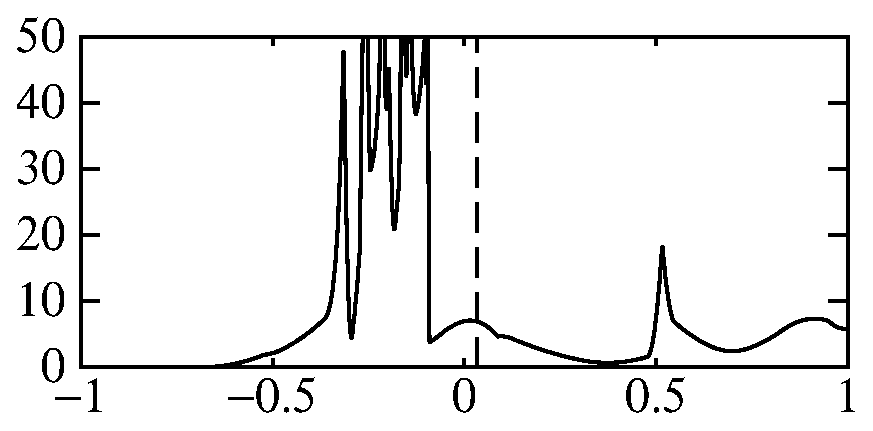
\includegraphics[width=70mm]{img/doscu.eps}
  \vspace{5mm}
  \caption{DOS(Cu)}
 \end{center}
\end{figure}
The range of DOS and division of total DOS is given by
DOSMAX and NPTS in ctrl. Edit tdos.cu.glt for gnulot for your presentation. 
Please look into \io{job\_tdos} file in your bin directory. It is a small script.

For band plot, we have to set symmetry lines along which we plot eigenvalues.
Collections \verb+syml.*+ are in ecalj/MATERIALS/. 
Choose and modify one of them and rename it. 
I will gather other samples soon. 'BZ wikipedia' or something else
will help you to interpret it.

To do band plot, we need \verb+syml.cu+ in your directory.
\begin{verbatim}
   $ cp ~/ecalj/MATERIALS/Cu/syml.cu .
\end{verbatim}
Then check \verb+syml.cu+; it is
\begin{verbatim}
    21  .5 .5 .5     0  0 0   L Gamma
    21   0  0  0     1  0 0   Gamma X
    0   (this is the terminator line)
\end{verbatim}
We supply ten data for each lines
(integer, three real, three real, two words).
First line means, we calculate eigenvalues 
for {\bf k} points from {\bf k}=(0.5,0.5,0.5) to {\bf k}=(0,0,0).
"L Gamma" are names of two end points 
(.5 .5 .5) and (0 0 0) in this case.
These names are used in a gnuplot script for band plot
(bndplot.isp*.glt).
Second line means, we calculate eigenvalues 
for k points from {\bf k}=(0,0,0) to {\bf k}=(1,0,0).
3rd line means calculation just stop here.
Units of {\bf k} are in 2$\pi/$\verb+ALAT+ (or 2$\pi/$\verb#(ALAT+DALAT)#
if \verb+DALAT+ exist.).
A line starting from '\#' is neglected (comment line).

To do band plot, run
\begin{verbatim}
    $ job_band cu
\end{verbatim}
. This is for both nspin=1 and nspin=2
(These scripts try to determine the Fermi energy first. You may skip it
in cases (but need to change the script)).

\begin{figure}[h]
 \begin{center}
  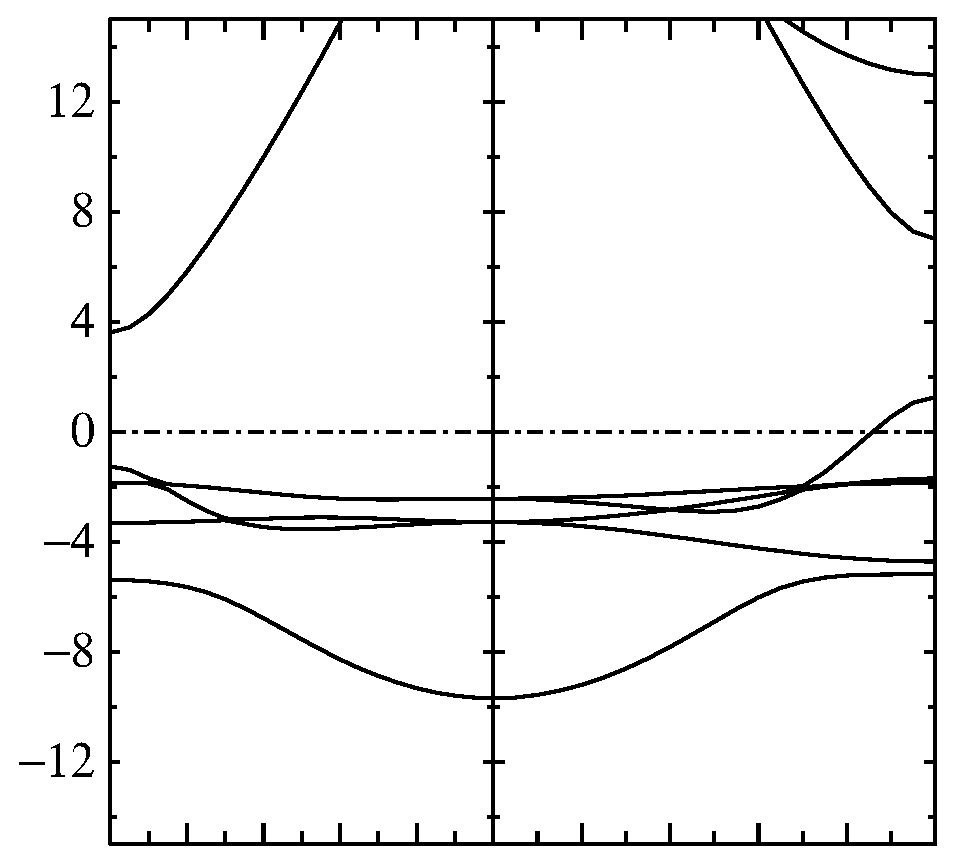
\includegraphics[width=70mm]{img/bandcu.eps}
  \caption{band plot(Cu)}
 \end{center}
\end{figure}

For PDOS plot,
\begin{verbatim}
    job_pdos cu
\end{verbatim}
It shows figures (number of figures are number of atoms in the cell) in
gnuplot (they are written in the same position on X-window;
move top one a little). The command \verb+job_pdos+ is a little 
time-consuming because we use no symmetry to distinguish all lm channels.
(PDOS is not yet implemented for SO=1 case; spin-orbit coupling $\L\dot S$ is added.)
We can edit script of gnuplot (pdos.site*.*.glt) for your purpose.
To plot again, run
\begin{verbatim}
  gnuplot -persist pdos.site001.cu.glt
\end{verbatim}
In principle, meanings of all data files are shown (see at the bottom
of console output about lm ordering in a line), thus not so difficult to
rewrite *.glt. For example, to plot eg and t2g separately. 
(NOTE: site id is shown by lmchk).\\

\noindent {\bf WARNING}: 
Usually lmf and so on recognize options such as -v option. For example,
' lmf gaas -vnspin=2' or 'lmf gaas -vso=1'. 
This option changes values of variables defined in \verb+% const+ section.
This is recorded in save.* file, and also shown at the top of console output. 
However, job\_tdos and so on, do not yet accept these options.
Thus we need to modify ctrl file without using -v option.
Or you need to write these option to these command by hand
(we will fix this problem in future.)

%\paragraph{Practice}
%Let start from scratch. 
%Make directory as \verb+~/ecaljtest/Si+ 
%And make \verb+ctrls.si+ first.
%Then generates \verb+ctrl.si+, and run lmfa, lmf successively. 
%There are other sample. Try it by yourself.


\subsection{Useful samples: ecalj/MATERIAL/}
Not only \verb+ecalj/lm7K/TestSamples+ (some of them are by older version),
We have a material database in \verb+ecalj/MATERIALS/+. 
Move to the directory, and type  
\begin{verbatim}
  $ ./job_materials.py
\end{verbatim}
Then it shows a help. You see 
\begin{verbatim}
...
=== Materials in Materials.ctrls.database are:===
  2hSiC  3cSiC  4hSiC  AlAs  AlN  AlNzb  AlP  AlSb  Bi2Te3  C
  CdO  CdS  CdSe  CdTe  Ce  Cu  Fe  GaAs  GaAs_so  GaN
  GaNzb  GaP  GaSb  Ge  HfO2  HgO  HgS  HgSe  HgTe  InAs
  InN  InNzb  InP  InSb  LaGaO3  Li  MgO  MgS  MgSe  MgTe
  Ni  NiO  PbS  PbTe  Si  SiO2c  Sn  SrTiO3  SrVO3  YMn2
  ZnO  ZnS  ZnSe  ZnTe  ZrO2  wCdS  wZnS
...
\end{verbatim}
. For these simple materials (now 57 materials), input files can be generated,
and run them automatically by a command \verb+./job_materials.py+ below.
The ctrls are stored in \verb+ecalj/MATERIALS/Materials.ctrls.database+
in a compact manner
(in addition, options passed to ctrlgenM1.py and options to lmf-MPIK are
included). See \verb+ecalj/MATERIALS/README+ about how to add new
material to it; it is not difficult. 
The command \verb+./job_materials.py+ gives ctrls.* for these materials
from descriptions in the \verb+Materials.ctrls.database+.
And then it generates ctrl file by calling ctrlgenM1.py internally, 
and run lmfa lmf-MPIK successively (when no --noexec).

Try \verb+./job_materials.py Fe --noexec+. (not fe but Fe as it shown above)
at \verb+ecalj/MATERIALS/+. 
Then it makes a directory Fe/ and set ctrl.fe (also ctrls.fe) in the
directory. Without '--noexec', it does calculation for Fe successively.
As for NiO and Fe, we see that \verb+./job_materials.py+ gives
SPEC\_ATOM\_MMOM in generated ctrls and ctrl files.
(Look into ctrls.fe; we need SPEC section when we add MMOM.)

Try \verb+job_materials.py GaAs Si+.\\
Then directories GaAs/ and Si/ are generated. See \verb+save.*+ files containing
total energies iteration by iteration. Starting from \verb+ctrl.*+ in
these directory, the command perform DFT calculations 
(Console output is stored in \verb+llmf+, \verb+save.*+ gives
total energies. \verb+rst.*+ contains self-consistent
density, from which we can calculate energy bands and so on).

``\verb+./job_materials --all --noexec+'' generates ctrls and ctrl files of
these materials. ``\verb+./job_materials --all+'' do self-consistent
LDA calculations for materials (it takes an hour or more. To change the
number of cores for lmf-MPIK, set option -np (number of core). See
help of \verb+./job_materials+ (type this without arguments).\\

To make band plot and so on for Fe, follow instructions already explained.
\begin{verbatim}
  $ ./job_materials.py Fe  (and need to type return)
  (If you like start over, remove Fe/ under it first).
  $ cd Fe
  $ ./job_materials.py fe
    (but it might be better to do --noexec, and observe Fe/ctrls.fe and
	Fe/ctrl.fe first. grep conf llmf shows the initial electron distribution).
  $ cat save.fe  (this shows total energies of each iteration. 'c ' at
	the first column gives converged result. 'h ' is from atm file.)
        If it does not ends with 'c ...' line, something strange
	occurs. see llmf (console out put of lmf is saved to llmf).
  $ cp ../syml.fe .
  $ job_band fe -np 4 
        (As I said, this shell script do not yet accept
	    options to lmf. Look into the script).
        (This calculate fermi energy first for safe; it takes
	    some time)       
  $ job_tdos fe
  $ job_pdos fe (as I said, this supress space-group symmetry, thus time consuming).
\end{verbatim}
At the end of \verb+job_pdos+, we show a help which pdos data is where
(In pdos file, we have 26 numbers a line; first is energy, 2-26 are pdos
for s,p,d,f,g; which is which are shown in the help).
See joblmf file also (it contains options to invoke lmf. This is shown
in save.*. In principle, options in joblmf should be passed to band plot
and so on. But not yet implemented 
(it is not so difficult; I have to do it).

After doing \verb+./job_materials+ foobar, you may like move it back to
original... In such a case, git works. At \verb+ecalj/+, do
\begin{verbatim}
  $ mv MATERIALS MATERIALS.bk
  $ git checkout MATERIALS
\end{verbatim}
Then you can see \verb+MATERIALS/+ is moved back to just downloaded one.



%%%%%%%%%%%%%%%%%%%%%%%%%%%%%%%%%%%%%%%%%%%%%%%%%%%%%%%%%
\subsection{How to add spin-orbit coupling?}
\begin{verbatim}
In the LDA level calculations, we can use
SO=0 (no SO), SO=1(LdotS), or SO=2(LzSz) schemes.
However, SO=1 is not the non-collinear method
(z-direction is assumed to be spin direction; in cases
we may need to primitive cell so that the z-direction
is the spin direction).

Within LDA, we have two possible ways.
(A) Do LDA and/or QSGW with SO=0 first.
Then apply the spin-orbit coupling by perturbation.
or (B) do self-consitent LDA calculations with SO=1 (or =2).
For semiconductors, we think you observe little differences.

Let me explain the case (A).
After converged with nspin=1, create new directory and copy
  ctrl.gas, rst.gas, sigm.gas, QGpsi,
to it. Then we set
  nspin=2 
  METAL=3 (usually this is default)
  SO=1  (this is ldots calculation off-diagonal elements included).
  Q=band (we do not change potential.)
in ctrl.gas. 
Then run
>lmf gas >& llmf_SO
You can see "band gap with SO" by 
> grep gap llmf_SO.
Then you can see two same lines.
  VBmax = 0.101949  CBmin = 0.236351  gap = 0.134402 Ry = 1.82786 eV
  VBmax = 0.101949  CBmin = 0.236351  gap = 0.134402 Ry = 1.82786 eV
(two lines per iteration is shown in metel mode).
This is the band gap with SO as a first-order perturbation 
on top of the "QSGW without SO". When you use ctrl fil e generated by
ctrlgenM1.py. You can do the above procedure with
>lmf --rs=1,0 gas -vnit=1 -vso=1 -vnspin=2 -vmetal=3 --quit=band
(--rs=1,0 read rst.gas but not write rst.gas. Run lmf --help.
 The switch -v (-vso=1 in this case) replaces so=0 with so=1. 
 This is recorded in save.gas file).

For band plot, you can use the same procedure 
for the case without SO. (Look into the shell script job_band.
You have to modify it so that 
  '--rs=1,0 gas -vnit=1 -vso=1 -vnspin=2 -vmetal=3 --quit=band' 
is added to arguments for >lmf --band:syml ...).
(--quit=band is not necessary if we like to renew eigenfunctions
self-consistent. Anyway we expect little differences.)

---

\noindent QSGW with SO:\\
For given sigm file, it is possible to attain self-consisency with SO=1(or=2) with keeping sigm (then we do not set Q=band). 
However, this imply that Vxc is fixed in QSGW, 
it is not necessary better than the above procedure.
\end{verbatim}


\subsection{PROCASR (VASP format) generator}
PROCASR mode for lmf (not yet in lmf-MPIK)
Band weight decomposition. 
(Size of circles show the size of components. Superposed on band
plot). See \verb#ecalj/MATERIALS/MgO_PROCAR/README#, May19.2014


\subsection{Effective mass calculation}
\begin{verbatim}
efermi.lmf:
this is generated by lmf(lmf-MPI), which is used in the job_band.

----------------
New band plot and effective mass calculation (curvature):
------------
We now read syml.* in lm7K/fp/bndfp.F. Thus job_band is changed
(nspin=1 or nspin=2 is automatically choosed by job_band command).
We do not use plbnd anymore. If necessary, you can modify
"writeband" subrouitne in lm7K/fp/bndfp.F by yourself.

Follow step to get effective mass...
1. 
New syml read label of k point. It is shown by the gnuscript
file "bandplot.glt". Type "gnuplot -p bandplot.isp1.glt" and so on,
when you like to remake band plot.

2. 
New syml allow a special input suitable to determine effective mass
for semiconductor. An example of new syml is (this is a case of GaAs)
------ syml example start ------------------
5  0 0 0   .5 .5  .5    Gamma  L
5  0 0 0    1.  0  0    Gamma  X
5  0 0 0   .75 .75 0    Gamma  K
#############
## resolution qinit qend iqinit iqend  etolv(Ry) etolc(Ry) symllabels
## mass*.spin* contains bands which is evaltop-etolv < eband <econtop+etolc
-888 !note -888 start Mass line. Here is a ZB case
257  0 0 0   .5 .5  .5   1   32     0.1 0.01    Gamma  L
257  0 0 0    1.  0  0   1   32     0.1 0.01    Gamma  X
257  0 0 0   .75 .75 0   1   32     0.1 0.01    Gamma  K
0 !terminator  
-------  end ----------------------
New feature is start from next line to the -888 line.
257 means a line connecting 0 0 0 (Gamma) and .5 .5 .5 (L) is divided
into 256. and we only calculate from the 1st point to the 16th point
among 513 points (now we need to include 1st point for mass).

We only make "Band001Syml005Spin1.mass" files which contains effective
math along the line only near the Fermi energy, that is,
we plot only bands whose energy E at Gamma (exactly speaking, at
left-end point), is evaltop-etolv < E < econtop + etolc.

(As its head line shows, Band*.mass file contains data
 isyml,iq, ib,isp, QPE-EF, QPE-QPE(start), |q|, mass=2*2*(QPE-QPE(start))/|q|**2).
 here QPE(start) is QPE at the left-end of sym line.)

For GaAs, please use this syml, and run job_band.
(e.g., job_band gaas -np 2 -vnspin=2 -vso=1; 
 note that -vfoobar=xxx replace value of foobar with xxx in ctrl.gaas)
Then you can see not only bandplot.isp1.glt, but also
massplot.isp1.glt, which is to plot data related to the last 3 lines
after -888. This is the effective mass plot for q points.
Note that what we need is at q to zero limit.

3. We have to make interpolation to q to zero.
In such a case, a possible way is "take average of degenerated bands,
and make an interpolation (least squrre fit by gnuplot).

4. least square fit by gnuplot. 

We have an example is at ~/ecalj/MATERIALS/mass_fit_test0.tar.gz
Expand this gives mass_fit_test0/. Look into ./job and run it. 
See README in it.
----
For your convenience, we have dE/dk in the bnd*.spin* files.
This is useful to determine the Fermi surface.
See the efermi.lmf to read the Fermi energy.

\end{verbatim}

\subsection{LDA+U, partially occupied core-hole}

\begin{verbatim}

See
file:///home/takao/ecalj/Document/BACKUP/MarksOriginalDoc/fp.html#ldaplusu
We need to add lines such as
  IDU= 0 0 2 2 UH= 0 0 0.1 0.632 JH= 0 0 0 0.055
for each SPEC_ATOM, And initial occnum.foobar file.
An example is in ecalj/MATERIALS/GdNldau/

When you just like to generate initial condition for gwsc,
you have to remove (or comment out) IDU before the 1st iteration
with sigm file, because sigm may already can contain LDA+U kind of effect.
(Thus you may need to modify gwsc or stop it at the 0th iteration,
and then remove IDU...)

Caution: 
We need the initial condition file such as occnum.gdn for LDA+U. 
(you may need to set "% real" at the begninig of the file).
Note that definition of spherical harmonics is in ecaljmanual.pdf.
(real harmonics is usual ones used in jobpdos).
Look for the keyword ldau in fp/lmfp.F -> sudmtu.F which read occnum.gdn.

\end{verbatim}


%%%%%%%%%%%%%%%%%%%%%%%%%%%%%%%%%%%%%%%%%%%%%%%%%%%%%%%
\section{How to run  QSGW calculation?}

In the QSGW, we calculate a 
{\it non-local exchange-correlation potential} $V^{\rm xc}(\bfr,\bfr')$,
by a procedure of GW calculation (very time-consuming part).
Then difference $V^{\rm xc}(\bfr,\bfr')V-V_{\rm xc}^{\rm
LDA}(\bfr)\delta(\bfr-\bfr')$  is stored into \io{sigm.*} file. 
The potential file \verb#sigm# is a key to perform QSGW calculations as seen in
Fig.\ref{gwscpicture}. The \verb#sigm# contains static non-local potential 
$\Sigma_{\rm QSGW}-V_{\rm xc}^{\rm LDA}$. 

Then, we again do one-body calculation by \exe{lmf} (or \exe{lmf-MPIK})
where we add this sigm to one-body potential ;
when we run \verb#lmf# or \verb#lmf-MPIK#(k-parallel mpi version),
\verb#sigm# is read and added to the one-body potential 
if we have \io{HAM\_RDSIG=12} in \io{ctrl.*}.
Thus this means that
we replace $V_{\rm xc}^{\rm LDA}(\bfr)\delta(\bfr-\bfr')$ 
with $V^{\rm xc}(\bfr,\bfr')$.\\

This iteration cycle is performed by a script ``gwsc'' as we
explain later on. (In the default setting of \verb+ctrl.*+ file, lmf try
to read sigm.* file as long as it exists. If not, do lmf or lmf-MPIK calculation.

To start QSGW calculation by \exe{gwsc},
we need not only \io{ctrl.si}, but also another input file \io{GWinput}.
Its template \io{GWinput.tmp} can be generated by the Step.2 as follows.

As a summary, you have to follow steps below in order to perform QSGW calculation.
\begin{enumerate}
\item[Step 1.] 
Perform from the Step.1 thru the Step.4 (up to lmfa) in Sec.\ref{lm7K-scf}.
(as same as the case of LDA/GGA).

You don't need to perform LDA calculation in advance,
since \exe{gwsc} perform LDA/GGA calculation at its beginning.
(It means that we start from the one-body Hamiltonian $H_0$ in LDA/GGA as initial condition.In cases, LDA/GGA give poor initial conditions for QSGW; in such a case,
we may need another trick to prepare starting point.).

[Caution: We have to use the same \verb#LMXA# ($l$ in the expansion of eigenfunctions 
in each MT) for all the MT spheres. (This is due to historical reason;
we may need to fix this.)]
xxx need to explain \verb#LMA# xxx

\item[Step 2.]\underline{Run the script \exe{mkGWIN\_lmf2}.}

The purpose of this script is to get \io{GWinput.tmp}.
Other files generated are not used in the following stage.

\item[Step 3.]\underline{Edit \io{GWinput.tmp} and save it as \io{GWinput}}.\\
\io{GWinput} is the input file describing the computational 
conditions for \GW calculation. 
Usually, the default setting gives reasonable results.
To reduce computational time, we may
use \verb#lcutmx(atom)=2# for oxygen sites 
(this may be also other small atoms.).
\verb#grep lcut GWinput -A1# shows \verb#lcutmx# for each atomic sites)
These step 2. and step 3. are just only to get \io{GWinput}.

\item[Step 4.]\underline{ Run the script \exe{gwsc}.}
\end{enumerate}


\subsection{GWinput}
\label{GWinput}
In order to perform QSGW, one another input file 
\verb+GWinput+ (no extension) is necessary in addition to \verb+ctrl.*+.
Thus all input files for QSGW is just two files, ctrl.* and GWinput.
A template \verb+GWinput+ can be generated by a script \verb+mkGWIN_lmf2+. 
You may have to modify it in cases for your purpose.\\

Let us start from ctrls.si;
\begin{verbatim}
#id  = Si
%const bohr=0.529177 a= 5.43095/bohr
STRUC
     ALAT={a} 
     PLAT=0 0.5 0.5  0.5 0 0.5  0.5 0.5 0 
SITE
     ATOM=Si POS=0.0 0.0 0.0
     ATOM=Si POS=0.25 0.25 0.25
\end{verbatim}
. Do \verb+ctrlgenM1.py si --tratio==1.0 --nk1=6+ and copy ctrlgenM1.ctrl.si to
ctrl.si. {\small NOTE: the option \verb@--tratio=1.0@ means we use touching MT; 
this can be checked by \verb+lmchk si+; since defaults is almost unity 
(\verb@--tratio=0.97@), this is irrelevant, just to explain options.} 

We have to write \verb+GWinput+. The default is given automatically by a
command \verb+mkGWIN_lmf2+;
\begin{verbatim}
    $ lmfa si (lmfa is needed to do in advance).
    $ mkGWIN_lmf2 si
    ......
    == Type three integers n1 n2 n3 for Brillowin Zone meshing for GW! ==
     n1=
\end{verbatim}
Then it pause and ask numbers. You have to type three numbers as
2+ return + 2+return+2 return.
\begin{verbatim}
    == Type three integers n1 n2 n3 for Brillowin Zone meshing for GW! ==
     n1= 2
     n2= 2
     n3= 2
    2 2 2
    ...(skip)...
    OK! GWinput.tmp is generated!
\end{verbatim}
Generated file is \verb+GWinput.tmp+; you have to copy it to \verb+GWinput+.
\begin{verbatim}
    $ cp GWinput.tmp GWinput
\end{verbatim}
These '2 2 2' you typed is reflected in a section 'n1n2n3 2 2 2 ' in
\verb+GWinput+. This means 2x2x2 (8 points in 1st BZ). 
You can edit it, and change it to e.g. 'n1n2n3 4 4 4' if you like to
calculate self-energy on dense BZ mesh 8x8x8. 

The template of GWinput is usually not so bad. But 
it may give a little expensive setting (or not very good enough in cases).


%%%%%%%%%%%%%%%%%%%%%%%%%%%%%%%%%%%%%%%%%%%%%%%%%%%%%%%%%%%%%%%%%%%
\subsection{Run gwsc script}
\label{fpgw-calc}
Let us perform QSGW calculation. 
For this purpose, we use a script \verb+gwsc+. 
We need to do \verb+lmfa+ in advance. Then do (not need to do \verb+lmf+);
\begin{verbatim}
    gwsc (number of iteration+1) -np (number of nodes) (id of ctrl)
\end{verbatim}
If (number of iteration+1)=0, it gives one-shot calculation from LDA.
But it is different from the usual one-shot;
since it calculates off-diagonal elements of self-energy also,
we can plot energy band dispersion. In cases (for usual
semiconductors), it can give rather reasonable results in comparison with
experiments from practical point of view.

This is an example of one iteration of QSGW cycle.
(now a little different but essentially similar)
\begin{verbatim}
takao@TT4:~/ecalj/test1$ gwsc 0 -np 2 si
gwsc 0 -np 2 si
### START gwsc: ITER= 0, MPI size=  2, TARGET= si
--- No sigm nor sigm.$TARGET files for starting ---
 ---- goto sc calculation with given sigma-vxc --- ix=,0
No sigm ---> LDA caculation for eigenfunctions 
        Start  mpirun -np 2 /home/takao/ecalj/TestInstall/bin/lmf-MPIK  si > llmf_lda 
OK! --> Start  echo 0| /home/takao/ecalj/TestInstall/bin/lmfgw si > llmfgw00 
OK! --> Start  echo 1|/home/takao/ecalj/TestInstall/bin/qg4gw > lqg4gw 
OK! --> Start  echo 1|mpirun -np 2 /home/takao/ecalj/TestInstall/bin/lmfgw-MPIK  si> llmfgw01 
OK! --> Start  /home/takao/ecalj/TestInstall/bin/lmf2gw >llmf2gw
OK! --> Start  echo 0|/home/takao/ecalj/TestInstall/bin/rdata4gw_v2  > lrdata4gw_v2 
OK! --> Start  echo 1| /home/takao/ecalj/TestInstall/bin/heftet > leftet 
OK! --> Start  echo 1| /home/takao/ecalj/TestInstall/bin/hchknw > lchknw 
OK! --> Start  echo 3| /home/takao/ecalj/TestInstall/bin/hbasfp0 > lbasC 
OK! --> Start  echo 3| mpirun -np 2 /home/takao/ecalj/TestInstall/bin/hvccfp0 > lvccC 
OK! --> Start  echo 3| mpirun -np 2 /home/takao/ecalj/TestInstall/bin/hsfp0_sc > lsxC 
OK! --> Start  echo 0|/home/takao/ecalj/TestInstall/bin/hbasfp0  > lbas 
OK! --> Start  echo 0| mpirun -np 2 /home/takao/ecalj/TestInstall/bin/hvccfp0  > lvcc 
OK! --> Start  echo 1|  mpirun -np 2 /home/takao/ecalj/TestInstall/bin/hsfp0_sc > lsx 
OK! --> Start  echo 11|  mpirun -np 2 /home/takao/ecalj/TestInstall/bin/hx0fp0_sc > lx0 
OK! --> Start  echo 2|  mpirun -np 2 /home/takao/ecalj/TestInstall/bin/hsfp0_sc  > lsc 
OK! --> Start  echo 0|  /home/takao/ecalj/TestInstall/bin/hqpe_sc  > lqpe 
OK! --> == 0 iteration over ==
OK! --> Start  mpirun -np 2 /home/takao/ecalj/TestInstall/bin/lmf-MPIK  si > llmf_gwscend.0 
OK! ==== All calclation finished for gwsc 0 -np 2 si ====
\end{verbatim}
Here \verb+echo (integer)+ is readin in at the beginning of the code.
To see it, please look into gwsc script (gwsc is at
ecalj/fpgw/exec/ and copied to your bin/ by make install2). 
In anyway, this console output shows calculations finished normally.

Now we get rst.si and sigm.si file which contains (static version of) self-energy
minims $V_{\rm xc}^{\rm LDA}$.
What we did is the one-shot GW from LDA result; but note that we
calculate not only diagonal elements but also off-diagonal elements. 

We can write energy dispersion (band plot) in the same manner in LDA.
To do it, we need rst.si, sigm.si, ctrl.si, QGpsi.
(but QGpsi is quickly reproduced). After you have syml.si
(e.g. in ecalj/MATERIALS/), Do
\begin{verbatim}
    $ job_band si
\end{verbatim}

\begin{figure}[h]
 \begin{center}
  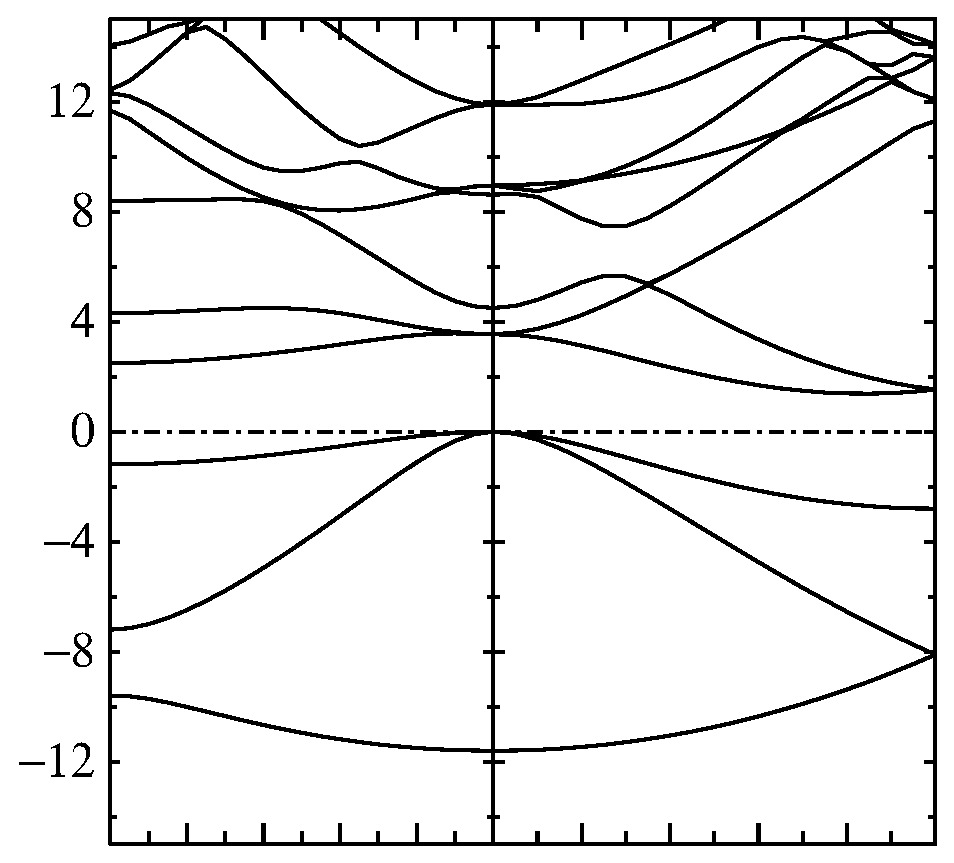
\includegraphics[width=70mm]{img/bandoneshotsi.eps}
  \caption{Si, one-shot GW with off-diagonal elements}
 \end{center}
\label{sigwscone}
\end{figure}
You can observe large band gap as shown in the Fig.\ref{sigwscone}.
(To see it again, \verb+gnuplot bnds.gnu.si -p+.
All plots are in gnuplot, thus it is easy to replot it as you like).

We have QPU file (and also QPD for spin=2), which contains content
of the diagonal part of self-energy. It will be explained elsewhere.

You can make total DOS and PDOS plot by 
\begin{verbatim}
    $ job_tdos si
    $ job_pdos si
\end{verbatim}
CAUTION:pdos plot is not allowed for so=1. (even tdos--> ask to t.kotani.)\\

To get final QSGW results, we have to repeat iteration 
until eigenvalues are converged.
Note that total energy shown by console output llmf (and also shown in
save file) is not so meaningful in the QSGW; we just take it as an indicator to check convergence. 
Let us repeat 5 iteration more. "-np 2" means one core to use.
\begin{verbatim}
$ gwsc 5 -np 2 si
### START gwsc: ITER= 5, MPI size=  2, TARGET= si
 --- sigm is used. sigm.$TARGET is softlink to it  ---
 ---- goto sc calculation with given sigma-vxc --- ix=,0
 we have sigm already, skip iter=0
 ---- goto sc calculation with given sigma-vxc --- ix=,1
 ...(skeip here) ...

OK! --> == 5 iteration over ==
OK! --> Start  mpirun -np 2 /home/takao/ecalj/TestInstall/bin/lmf-MPIK  si > llmf_gwscend.0 
OK! ==== All calclation finished for gwsc 0 -np 2 si ====
\end{verbatim}
Note that we do skip 0th iteration (it is for one-shot from LDA) since
we start from rst.si and sigm.si given by one-shot LDA.
Thus we do just five iterations.
Information of eigenvalues are in \verb+QPU.(number)run+ files.
(for magnetic systems with nspin=2), wee have \verb+QPD.(number)run+ also).
Check it by ls;
\begin{verbatim}
    $ ls QPU.*run
    QPU0.run  QPU.1run  QPU.2run  QPU.3run  QPU.4run  QPU.5run
\end{verbatim}
(These are overwritten when we again repeat gwsc; be careful.)
Note that \verb+QPU0.run+ was old one when you did 1-shot GW from LDA 
at the beginning. In anyway *.0run are confusing files; remove them).

In order to check convergence calculations going well during iteration, do
\begin{verbatim}
   $ grep gap llmf*
\end{verbatim}
This shows how band gap changes in llmf.*run files.
In metal cases, we need to compare QPU file, magnetic moment or
\verb+grep '[xc] save.*+; this shows end of lmf iteration.
Energy is not so meaningful but can be indicator to convergence.

Let us check convergence of the QSGW calculations.
For this purpose, it is convenient to take a difference of QPU(QPD) files
by a script \verb+dqpu+. These files are human readable.
To compare \verb+QPU4.run+ and \verb+QPU5.run+, do
\begin{verbatim}
    $ dqpu QPU.3run QPU.4run
\end{verbatim}
Then we see a list of numbers (these are the differences of values in
QPU files).  Then it shows at the bottom as
\begin{verbatim}
    Error! Difference>2e-2 between:   QPU.4run   and   QPU.5run  
    :  sum(abs(QPU-QPD))= 0.05736
\end{verbatim}
but you don't need to care it so much.
You rather need to check the difference of values.
I can say most of all difference (especially around the Fermi energy are
) are almost 0.00eV or 0.01eV, we can judge QPEs are converged.
If not converged well, you may need to repeat 
\verb+gwsc+ again.
(when the size of two QPU files are different, dqpu stops.)

\begin{figure}[h]
 \begin{center}
  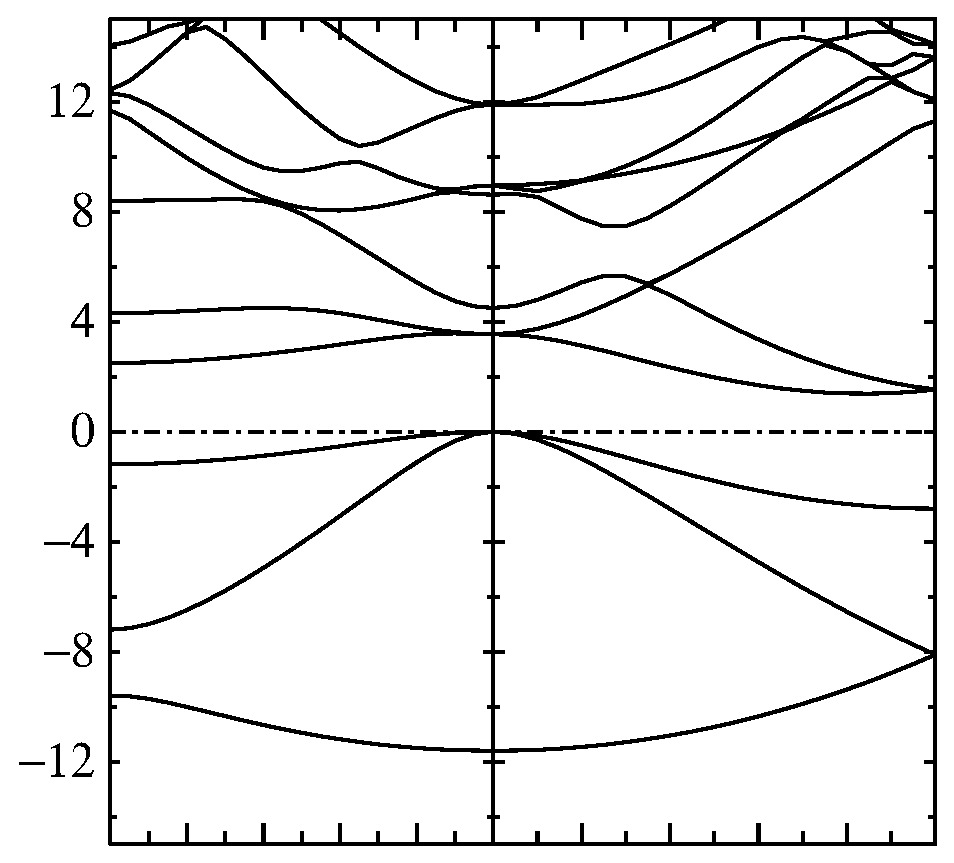
\includegraphics[width=60mm]{img/bandoneshotsi.eps}
  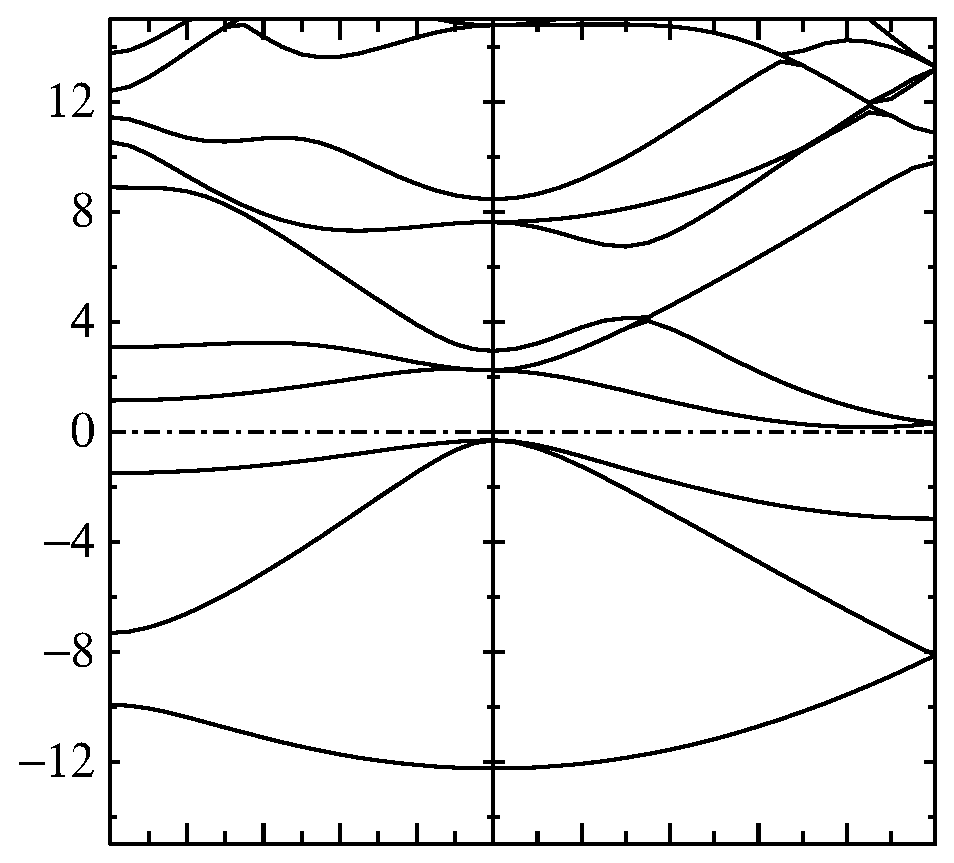
\includegraphics[width=60mm]{img/bandggasi.eps}
  \caption{band plot(Si, QSGW one-shot test)    and    band(Si) (GGA)}
 \end{center}
\end{figure}

%\paragraph{practice}
%Perform QSGW calculation for GaAs.
%Try one-shot GW, and plot it first.
%Then do QSGW. You can try 'n1n2n3 4 4 4', it is a little time
%consuming (maybe about 30 minutes per iteration or more).

%\begin{figure}[hbtp]
%  \includegraphics[width=60mm]{img/ps.dos.gga.si}\hspace{10mm}
%\end{figure}

\begin{figure}[hbtp]
  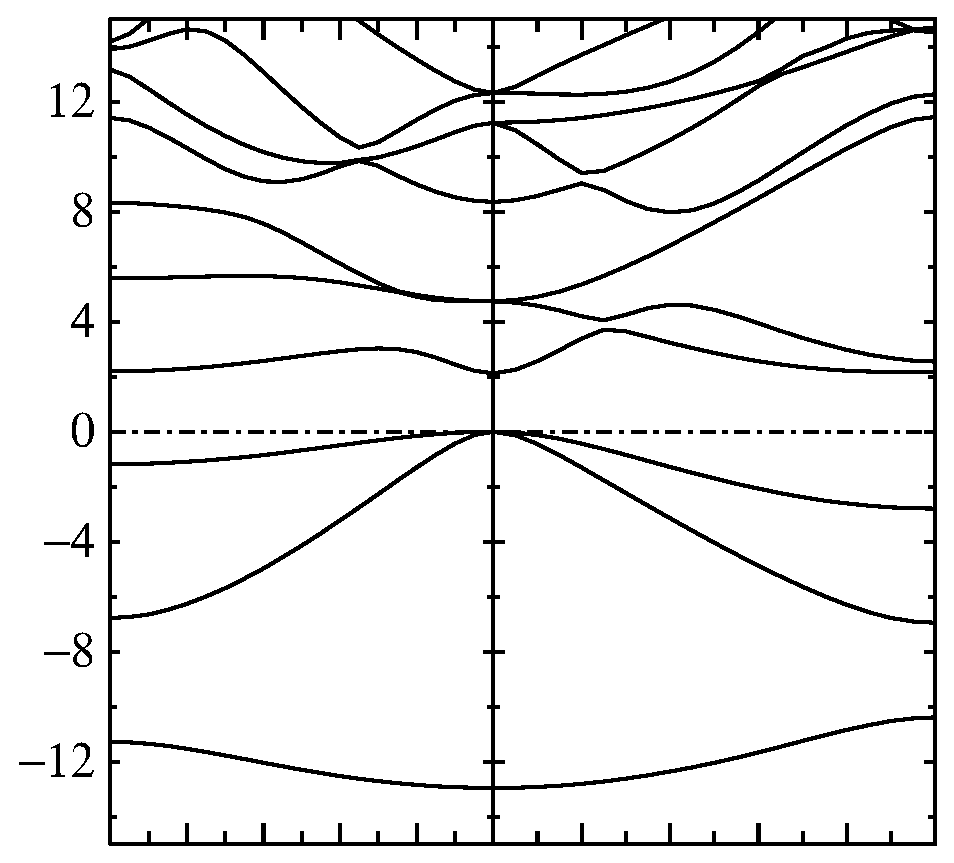
\includegraphics[width=60mm]{img/bandqsgwgaas.eps}
  \caption{band(GaAs), QSGW (test case)}
\end{figure}

%\section{calculation of dielectric function}
%  eps mode.

\subsection{Spectrum function: How to calculate <ki|Sigma(omega)|ki>}
\begin{verbatim}
How to do it?
1. Set <QPNT> section.
2. Run gwsigma or 
   Stop sc calculation after dielectric funciton, and run 
   echo 4| mpirun -np 24 hsfp0.
   Then we have SEComg.UP (DN) files, Look for file handle, ifoutsec,
   for the file in fpgw/main/hsfp0.sc.F to see format for the file.
3. Be careful about dw and omg_c.
   (We may not have good accuracy at high energy).
   We calculate weight of imaginary part along imaginary axis.

There is an example MATERIALS/SiSigma/
(To generate accurate Sigma(omega),
  we need to enlarge n1n2n3, and maybe with denser mesh (setting of dw, omg_c).)

\end{verbatim}

%%%%%%%%%%%%%%%%%%%%%%%%%%%%%%%%%%%%%%%%%%%%%%%%%%%%%%%%%%%%%%%%%%%%%
\newpage
\section{gwsc script to perform QSGW}
\label{gwsc}

\subsection{outputs of \exe{gwsc}}

\begin{figure}[h]
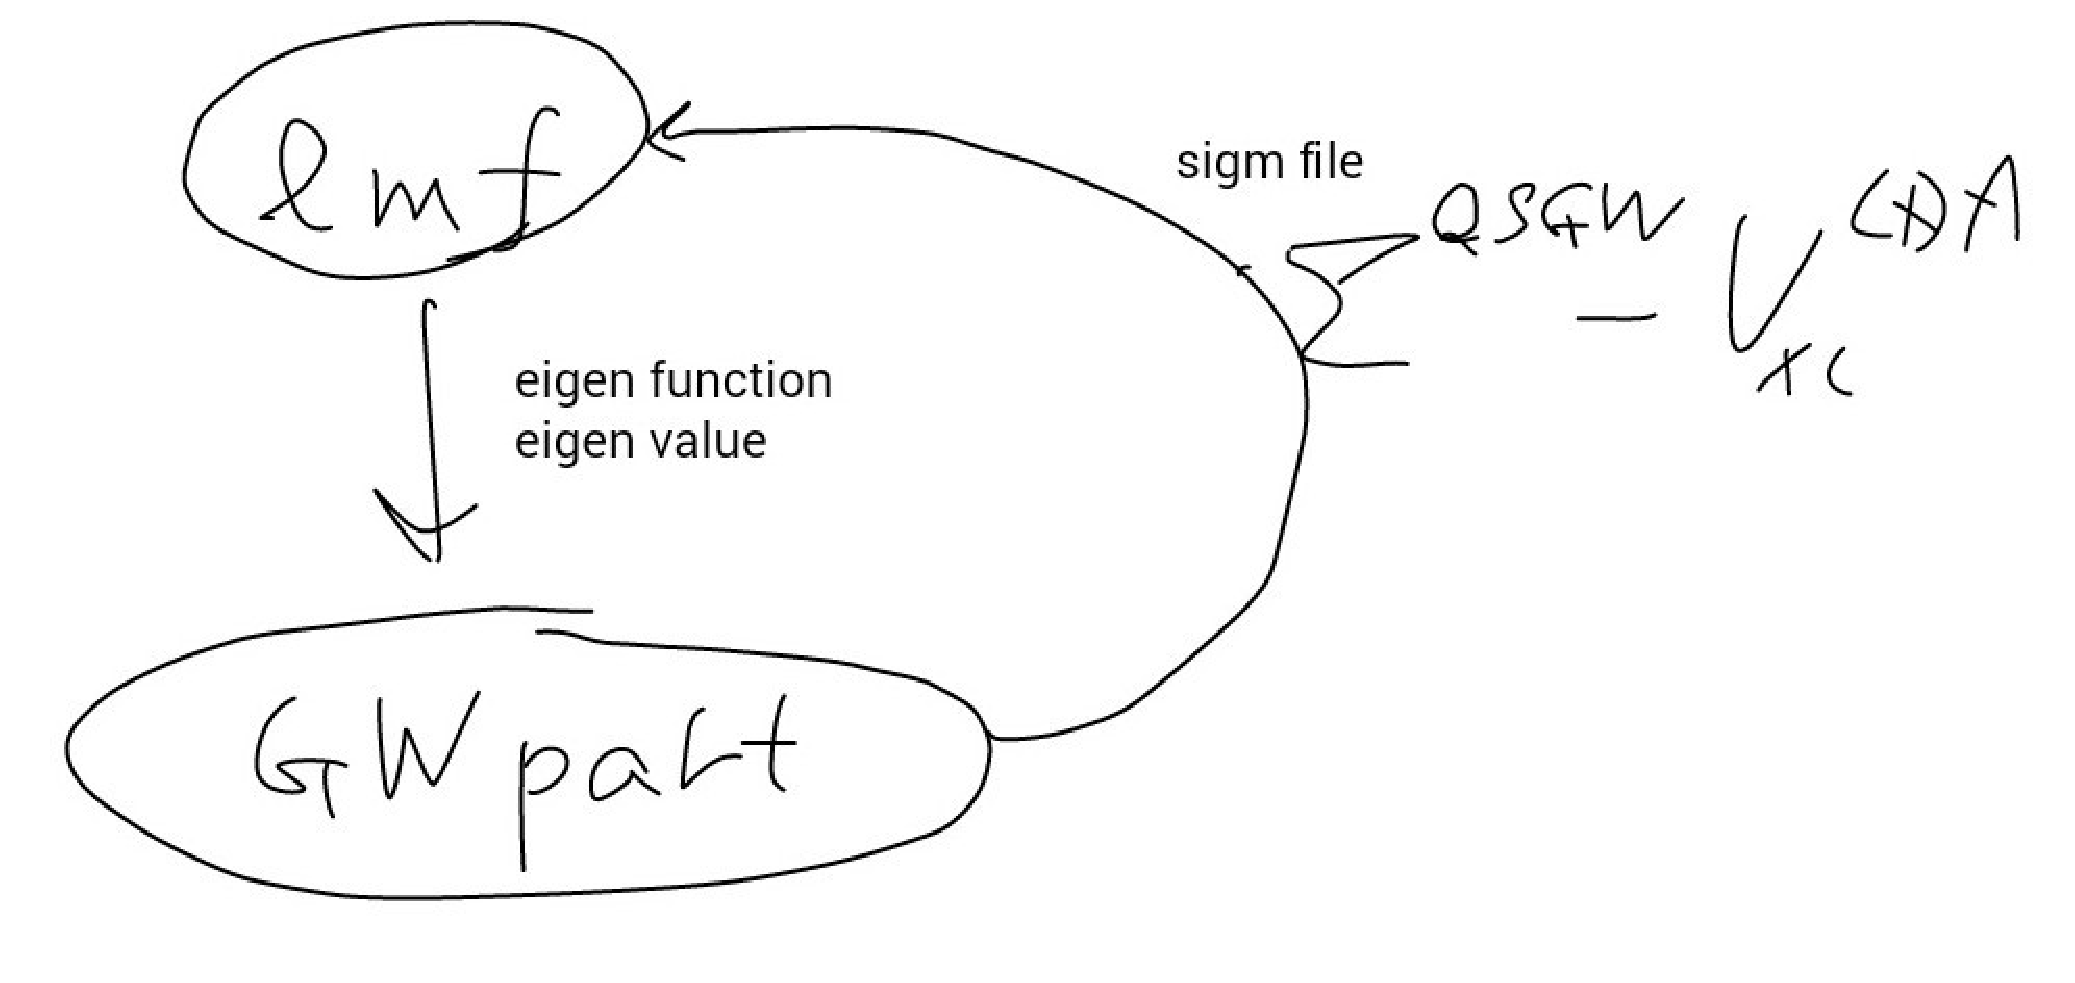
\includegraphics[width=10cm]{gwsc2014-12-091.eps}
\caption[]{Shell script {\tt gwsc} to perform \QSGW contains 
an iteration loop to make sigm (and eigenvalues, eigenfunctions)
self-consistent. The iteration loop is written in 
ecalj/fpgw/exec/gwsc (a bash script). 
Exactly speaking, we have to pass all the required data 
(not only eigenvalues and eigenfunctions, but also 
crystal structure, {\bf q+G} vectors, symmetry information and so on) to GW part.
The purpose of the GW part is to calculate $\Sigma_{\rm QSGW}-V_{\rm xc}^{\rm LDA}$.}
\label{gwscpicture}
\end{figure}

When \exe{gwsc} runs normally, it gives console output as follows.
This is a case for \io{ctrl.gaas} for\\
\verb#>gwsc 10 -np 24 gaas#\\
. Without arguments, typing \exe{gwsc} shows usage as \\
\verb#>An example of usage: gwsc 5 -np 4 si, where 5 means 5+1 iterations#\\
. We recommend you do look into the script \exe{gwsc}. 
It uses \io{run\_arg}, which is a special
subroutine of bash; but not so difficult to understand it.
(In the followings, we assume \io{/home/binx/} is your bin directory 
at which we have all binaries for ecalj.)

%\begin{mspace}
{\baselineskip=2mm
\begin{verbatim}
### START gwsc: ITER= 10, MPI size=  24, TARGET= gaas
--- No sigm nor sigm.$TARGET files for starting ---
 ---- goto sc calculation for given sigma-vxc --- ix=,0
No sigm ---> LDA caculation for eigenfunctions 
OK! --> Start echo --- | mpirun -np 24 /home/binx/lmf-MPIK gaas > llmf_lda 
OK! --> Start echo 0 | /home/binx/lmfgw gaas > llmfgw00 
OK! --> Start echo 1 | /home/binx/qg4gw  > lqg4gw 
OK! --> Start echo 1 | mpirun -np 24 /home/binx/lmfgw-MPIK gaas > llmfgw01 
OK! --> Start echo --- | /home/binx/lmf2gw  > llmf2gw 
 ... (preparation stage ends here; start main stage) ...
OK! --> Start echo 0 | /home/binx/rdata4gw_v2  > lrdata4gw_v2 
OK! --> Start echo 1 | /home/binx/heftet  > leftet 
OK! --> Start echo 1 | /home/binx/hchknw  > lchknw 
OK! --> Start echo 3 | /home/binx/hbasfp0  > lbasC 
OK! --> Start echo 3 | mpirun -np 24 /home/binx/hvccfp0  > lvccC 
OK! --> Start echo 3 | mpirun -np 24 /home/binx/hsfp0_sc  > lsxC 
OK! --> Start echo 0 | /home/binx/hbasfp0  > lbas 
OK! --> Start echo 0 | mpirun -np 24 /home/binx/hvccfp0  > lvcc 
OK! --> Start echo 1 | mpirun -np 24 /home/binx/hsfp0_sc  > lsx 
OK! --> Start echo 11 | mpirun -np 24 /home/binx/hx0fp0_sc  > lx0 
OK! --> Start echo 2 | mpirun -np 24 /home/binx/hsfp0_sc  > lsc 
OK! --> Start echo 0 | /home/binx/hqpe_sc  > lqpe 
OK! --> Start echo --- | mpirun -np 24 /home/binx/lmf-MPIK gaas > llmf_oneshot 
  ... (this is the end of main stage) ...
== 0 iteration over ==
 ---- goto sc calculation for given sigma-vxc --- ix=,1
OK! --> Start echo --- | mpirun -np 24 /home/binx/lmf-MPIK gaas > llmf 
OK! --> Start echo 0 | /home/binx/lmfgw gaas > llmfgw00 
   ... (lines here omitted ) ...
OK! --> Start echo 0 | /home/binx/hqpe_sc  > lqpe 
== 1 iteration over ==
   ... (lines here omitted ). ..
== 2 iteration over ==
   ... (this repeat until ITER= 10(the first argument to gwsc) ) ...
\end{verbatim}
%\end{mspace}
}
This shows that \exe{gwsc} invoke \exe{lmf-MPIK,lmfgw,qg4gw,...} successively.
\exe{echo~3$|$hbasfp0 } means running a fortran program \exe{hbasfp0} 
with the argument '3' from the standard input (\io{read(*,*)} in fortran
code).
We can divide these successive calls to ``preparation stage'' and ``main
stage''. Preparation stage is just to prepare eigenfunctions and so on 
which are required for the ``main stage'' of GW calculation.
At the end of ``main stage'', we have the potential file \io{sigm}.

As it shows, console output are going to l* files.
%\item[Step 5.]
%\underline{\large Run the script {\bf hqpemetal} in the case of metal}
%
%This is in order to get the correct Fermi energy by the tetrahedron method.
%
%(To execute {\bf hqpemetal}, you need to calculate all the QP energies 
%at least just above the Fermi energy).
%
%[this is for old users: Note that the newer {\bf hqpemetal} will not work for old results by fpgw020;
%you need to change \verb#nnv# in {\sf LMTO} file.]

%In the case of the Antiferro materials, the compuational efforts reduced to be half 
%(only hx0fp0 part; most expensive for one-shot $GW$) if you prepare a file {\sf Anfcond} 
%by handbefore you execute {\bf gw\_lmfh}. See next section for it.
%(this function now works only for the case that 
%a symmetry operation is [a translation verctor with spin inversion].)

%Unix shell scripts {\bf gw\_lmf} in the {\tt ecal/fpgw/exec} directory
%makes the procedure almost automatic.
%{\bf gw\_lmf} is for the \GW calculation including cores.
%{\bf gwnc\_{\it foo}} is for the \GW calculation without core.
%{\it foo} donotes the LDA method;we now have 
%implimented {\bf gw\_nfp}, {\bf gwnc\_nfp}, and {\bf gw\_lmf}.


%In anyway, it is necessary to look into these shell scripts, 
%and observe the cosole outputs of each programs called from the script 
%(they are usually reserved to \io{l*} files,e.g. \io{lbas} or so. 
%Look into the scripts.) You don't need to understand all items in console outputs;
%I am sloppy to orgainize it--- so, not so meanigful or debugging check write are 
%in these console outputs.


\vspace{3mm}
\subsection{\bf Preparation stage of \exe{gwsc}}
At the end of this stage, 
we get required eigenfunctions, BZmesh data, and so on,
which are required for the main stage.
Note that 
{\bf echo 0 $|$ lmfgw} means supply an integer to the fortran program
{\bf lmfgw} from standard input by read(*,*).
\begin{itemize}
\item \exe{lmf-MPIK} (k-parallel version of \exe{lmf})\\
This is the one-body calculation for given \io{sigm.gaas}.
At the beginning, we do not have \io{sigm.gaas}.
In this case \exe{lmf-MPIK} just perform LDA/GGA calculation. 
\item{\bf echo 0 $|$ lmfgw}: \\
  Get some small information files to start {\bf qg4gw}.
  If you type just lmfgw, and observe what occurs.
  It shows a menu and pauses (asking you to supply an integer); then
  we supply 0 in this case. (If we do {\bf echo 0 $|$ lmfgw}, no pause occurs.)
\item{\bf echo 1 $|$qg4gw }: Get ${\bf k}$ points used
  in the \GW calculations and the corresponding ${\bf G}$ vectors.
  And what is the irreducible k point (See console output of qg4gw.
  \exe{gwsc} keeps it in \io{lqg4gw}).\\
  Since we use the offset-Gamma method for BZ integration for $G \times W$,
  we need shifted mesh points to calculate $W$ at offset-Gamma points.
  The $\bfq$ vectors of offset-Gamma method is in \io{Q0P} file.
  (If you have two points in \io{Q0P}, we see two shifted mesh points in
   addition to regular mesh points.)
  Remember that cutoff of ${\bf G}$ is given by QpGcut\_psi and QpGcut\_cou
  in \io{GWinput}. (Based on the experiences, we use smaller QpGcut\_cou
  to reduce computational time. Explained in other section xxx).
\item{\bf echo 1 $|$ lmfgw-MPIK} : 
 Calculate the LDA eigenfunctions, eigenvalues, and
 $\langle \psi | V^{\rm LDA}_{\rm xc}| \psi \rangle$
 at the irreducible ${\bf k}$ points (shown at the bottom of output
     \io{lqg4gw} of \exe{qg4gw}.)
\item{\bf lmf2gw}: store these data into {\sf DATA4GW\_V2} and {\sf CphiGeig}, 
whose I/O is controlled by a key subroutine {\bf gwinput\_v2.f}.
\end{itemize}

\subsection{\bf Main stage of \exe{gwsc}}
\label{mainstage}
We can start the main stage of \GW calculation from these files;\\
\verb#GWinput DATA4GW_V2 CphiGeig QGpsi QGcou Q0P QIBZ SYMOPS BZDATA HAMindex CLASS#;\\
\noindent these files contains eigenfunctions and so on in the manner 
of Eq.(17) of \cite{kotani_quasiparticle_2014}, eigenvalues and other required
information. This is the starting point of the GW calculation.\\

{\baselineskip=5mm

\fl{GWinput} computational conditions.

\fl{DATA4GW\_V2} Crystal structures and so.

\fl{CphiGeig} Eigenvalues and Eigenfunctions

\fl{QGpsi} q and G vector for the eigenfunctions(q means {\bf k} in the previous section),

\fl{QGcou} q and G vector for the Coulomb matrix

\fl{Q0P}   q points near q=0 instead of q=0 (offset Gamma points)

\fl{QIBZ}  irreducible q points (This is also contained in {\sf BZDATA}).

\fl{SYMOPS} point group operation

\fl{BZDATA} q points date (and tetrahedron weights if necessary) for BZ integrals.

\fl{HAMindex} Hamiltonian index, all required complex index for Hamiltonian of PMT method.
(See the top of \io{subroutine write\_hamindex} in \io{lm7K/subs/m\_hamindex.F}. 
This is also in \io{fpgw/gwsrc/m\_hamindex.F}. Identical files are in two
different directory--- it should be avoided in future.)

\fl{CLASS} class information or atomic sites (equivalent sites).\\


With these files, we do the main stage as

\begin{itemize}
\item{\bf rdata4gw\_V2}: 
  Read {\sf DATA4GW\_V2} and so on, and decompose it into files required
     in the followings. And calculate PPOVL* files (overlap matrix of
     interstitial plane waves. Because of technical reasons some
     different types of PPOVL* with \bfq-point index).
\item{\bf heftet   }: Get the Fermi energy {\sf EFERMI} by tetrahedron method. It is used in {\bf hx0fp0}.
\item{\bf hchknw   }: stores the number of required $\omega$ points along real-axis into {\sf NW}. \\
{\small ({\sf NW} is not essentially used, but is supposed to exist in the followings.)}
\item{\bf echo 3$|$hbasfp0}: gives the product basis for Core exchange.
\item{\bf echo 0$|$hvccfp0}: gives the Coulomb matrix for the Core exchange.
\item{\bf echo 3$|$hsfp0\_sc  }: gives the Core exchange part of the
     self-energy. \footnote{Correlation part due to cores is neglected.
     In future, we will switch to a version without PB for core part to
     reduce computational time and for numerical accuracy.}
\item{\bf echo 0$|$hbasfp0}: gives the product basis.
\item{\bf echo 0$|$hvccfp0}: gives the Coulomb matrix $v$.
\item{\bf echo 1$|$hsfp0\_sc  }: gives the exchange part of the self-energy.
\item{\bf echo 11$|$hx0fp0\_sc }: gives the correlated part of the screened Coulomb interaction $W-v$.
\item{\bf echo 2$|$hsfp0\_sc  }: gives the correlated part of the self-energy.
\item{\bf echo 0$|$hqpe\_sc}: gather data and write down final results
     into {\sf sigm}, {\sf QPU}, {\sf TOTE.UP} files.
\end{itemize}
\vspace{.3cm}

%Then you can do the script {\bf hqpemetal} in the case of metal in order to get
%the Fermi energy for the QP energies.


\vspace{3mm}
\subsection{\bf Other functions (or scripts)}
In addition to {\bf gw\_lmfh}, there are some other additional scripts 
and functions.

\begin{itemize}
\item
{\bf gw\_lmfh} : The one-shot \GW calculation. 
     Lifetime(impact ionization rate) of QPs.

\item
{\bf gwsc} : QSGW calculation explained here

\item
{\bf \ epsPP\_lmfh, eps\_lmfh} : Dielectric function without or with local-field effects.

\item
 run-mode 4 of {\bf hsfp0}: to plot the spectrum function
     $\Sigma(\omega)$.(need to be fixed again probably). 

%\item
%{\bf gwband\_lmf} : for plotting band (not well maintained now).

\item
{\bf epsPP\_lmfh\_chipm} : non-interacting spin susceptibility. 
One-degree of freedom like Rigid moment approx.
After it ends, you need to do \verb#calj_nlfc_metal# and/or \verb#calj_summary_mat#
to get the full spin susceptibility.

\item
{\bf genMLWF} : Wannier funciton and its matrix elements of the Screened
     Coulomb interaction.

\end{itemize}

% Scripts below are for tests 
% \begin{itemize}
% \item
% {\bf extest, \ extest\_repeat}: 
% which is in order to check the dependence of $\Sigma_{\rm x}$ as for $E_{\rm smear}$.

% {\bf gw\_lmf} : The one-shot \GW calculation, older version. \\
% (Direct calculation of the polarization function
% without going through the Hilbert-transformation.

% \item
% {\bf \ eps\_lmf}   : Dielectric function with local-field effects. 
% Direct mode(Not Hilbert-transformation).

% \item
% {\bf gwpara\_lmf} : A test gw script for parallel computing (testing. it may not work now).

% \item
% {\bf eps\_lmfh\_chipm} : spin susceptibility (full mixed basis). Test purpose.
% \end{itemize}

\section{Cautions for usage}
\label{cautionusage}
\begin{enumerate}
 \item == not meaningful total energy in QSGW===\\
 Total energy shown in QSGW mode in current version is not meaningful. 
(just treat as an indicator to convergence).

\item == Do we use VWN or GGA for QSGW? ===\\
  In principle, QSGW results should not depends on VWN or GGA 
  (XCFUN=1 or 103 in ctrl). But there is minor dependence, because\\
   1. frozen core density.\\
   2. core eigenfunctions.\\
   3. radial basis functions\\
   4. Slight numerical reason \\
      (This is probably because Sigma-interpolation procedure
       But not exactly figured out yet
       $\rightarrow$ affect about 0.02eV as for band gap for GaAs. ).
  In anyway, use VWN (HAM\_XCFUN=1) as standard.
  And such technical things affects, 0.05 eV level of error for band gap.

\item{EH and EH2} : For si, if EH and EH2 are the same, the following
     error occurred. 
\begin{verbatim}
 fexit,fexit2,fexit3 error retval=          -1
 Exit -1 zhev_tk2: nev /=nevx something wrong.
\end{verbatim}
     The large EH, EH2 get to be meaningless. We usually use up to 
     $\sim 2$. (If you use very large EH such as E$\sim 10$, I am not so
     sure weather it is )

\item { The options about the product basis within MT. (SeungWoo's memo)}

\begin{verbatim}
<PRODUCT_BASIS>
 tolerance to remove products due to poor linear-independency
  0.100000D-02 ! =tolopt
\end{verbatim}
When the product basis are made, we may have poorly linear independent
basis. For example, one in the set \{$f_1, f_2, ..., f_n$\} would 
be almost give by a linear-combination of others. We need to make the
      linear-independent set. Therefore, after calculating the overlap matrix 
      $\langle  f_i|f_j \rangle$. We do diagonalization, then 
      we remove eigenvectors corresponding to small eigenvalues than
      \verb+tolopt+. 
      See the {\bf hbasfp0} command in {\bf gwsc}

\begin{verbatim}
lcutmx(atom) = maximum l-cutoff for the product basis.
  4  4  4  2  2  4  4
\end{verbatim}
For $\phi_1 \times \phi_2$ case, $|l_1 - l_2| \le l_{tot} \le |l_1 + l_2|$. So `lcutmx' changes the maximum cutoff for the l$_{tot}$. The order is the same as the order of atoms in the {\bf ctrl} file.

\begin{verbatim}
  atom   l  nnvv  nnc !
    1    0    3    3
    1    1    3    2
    1    2    2    1
\end{verbatim}
`atom' means the atom number identified in the {\bf ctrl} file.\\ 
`l' is the angular momentum quantum number.\\
`nnvv' is the number of radial functions (valence) on the augmentation-waves.\\
`nnc' is the number of radial functions for core.\\
The latter two ones, `nnvv' and `nnc', will be understood more clearly if you see the following ones.


\begin{verbatim}
  atom   l    n  occ unocc  ! Valence(1=yes,0=no)
    1    0    1    1    1   ! 5S_p  -----
    1    0    2    0    0   ! 5S_d
    1    0    3    1    1   ! 4S_l
    1    1    1    1    1   ! 5p_p
    1    1    2    0    0   ! 5p_d
    1    1    3    1    1   ! 4p_l
\end{verbatim}
Above options are about the product basis set within MT (Valence).\\
`atom' and `l' are explained above. `nnvv' for `atom = 1 and l = 0' was `3' so this case we have 3 basis (`n = 1, 2, 3')\\
`n' is the degree of freedom of the radial function, $\phi$. `n = 1'
      means $\phi$, `n = 2' means $\dot\phi$, and `n = 3' means kind of
      $\ddot\phi$, which the dot above the letter represents the
      differentiation with respect to the energy. So `n = 1 and 2' is
      related to the linearization of the radial function and `n = 3' is
      the local orbital which is restricted in MT. The local orbital can
      be modified changing `PZ' in the {\bf ctrl} file. Finally, the
      number of the basis set which is needed for expanding eigenfunctions is $(l+1)^2 \times n$.\\
`occ' and `unocc` mean that we use only ones that checked as `1', in other words we neglects `0' cases for making product basis. Be careful for confusion with name `occ' and `unocc'. These don't mean that occupied or unocc. When making product basis, $M = \phi_1 \times \phi_2$, `occ' corresponds to $\phi_1$ and `unocc' to $\phi_2$. For example, 
\begin{verbatim}
  atom   l    n  occ unocc  ! Valence(1=yes,0=no)
    1    0    1    1    1   ! 5S_p  -----
    2    3    1    0    1   ! 4f_p
\end{verbatim}
If the options are like the above, the product basis will be consists of ($\phi_1 = \phi_{atom=1,l=0}) \times (\phi_2 = \phi_{atom=1,l=0})$, ($\phi_{atom=1,l=0} \times \phi_{atom=2,l=3}$). As you can see, ($\phi_1 = \phi_{atom=2,l=3}$) is skipped.\\
In the {\bf ctrl} file, `EH' controls the l part. As for `EH', (s, p, d, f) are used but {\bf GWinput} file uses (s, p, d, f, g). `EH' : HEAD part. `GWinput' : contains TAIL part... need more explanation.

\begin{verbatim}
  atom   l    n  occ unocc  ForX0 ForSxc ! Core (1=yes, 0=no)
    1    0    1    0    0      0    0    ! 1S -----
    1    0    2    0    0      0    0    ! 2S
    1    0    3    0    0      0    0    ! 3S
\end{verbatim}
Above options are about the product basis set within MT (Core).\\
`nnc' for `atom = 1 and l = 0' was `3' so this case we have 3 basis (`n = 1, 2, 3')\\
Finally, for the convergence check, we can modify the following three things, (i) tolerance, (ii) lcutmx, and (iii) occ and unoccu.


\end{enumerate}
\begin{verbatim}


== one show QSGW (not one-shot GW) ==
  one-shot QSGW can be useful in cases.
  As it contains off-diagonal part, we can resolve band tanglement
  problem in Ge (no band gap).

== Restart calculation in lda ==
 lmf(lmf-MPIK) read rst.* in defaluts.
 rst contains electron density.
 If rst is already converged, it stops after two iteration.
 rst contains atomic positions.
 So, in order to read atomic positions change in ctrl,
 Use options shown in lmf --help.

== Restart calculation in qsgw ==
  To remove mixsigm* (mixing for sigm), maybe required.

== iteration check ===
  First, watch console output of gwsc (do redirect to output file)
  Need to check OK! signs arrayed on 1st columns.

  gwsc iteration is time cosuming,
  So we need to check calculations are normally going on or not.

  Memory inefficiency.
  Set 'KeepEigen off' an 'KeepPPOVL' off.
  In fact, out code is still inefficient for memory usage.
  
  grep gap llmf ---> minimum gap at mesh point.
  see save.* ,or grep '[xc] ' save.*
  the end of iteration of lmf is shown as x or c.
  (if failed, QPU file. 
  dqpu QPU.4run QPU.3run
  As for usual semi-conductor, accuracy abou t0.1 eV is limit of current implementation.
  Set vwn (xcfun=1) looks better (stable) for GW.

  $grep rms lqpe* 
  shows
           ...  rmsdel=2.44D-04
           ...  rmsdel=4.91D-03
           ...   rmsdel=2.44D-04
           ...   rmsdel=3.37D-04
  If rsmdel is getteing to be smaller, it is on convergence path.
  (but in magnetic cases, it may give be too good even not yet going to
	be converged..., beccause magnetic energy is so small)

  grep diffe llmf  ---> difference of energies of each iteration.

  ehf (harris energy)
  ehk (Hohenberg kohn energy)

== emax cutoff for APWs. ==
  We can not use so many APWs in current version,
  because of overcompleteness (this is because null vector within MTs), 
  In anyway, use pwemax=3 as standard (test it with 4 or 5).
  To avoid failure of calculation, we may use smaller MT radius for
  alkali, and alkali-earth elements. 
  In feature, I think we can introduce pseudopotentials for these atoms only.

== Check Used MTO 
 Near beginig of console output, what MTO you use is shown as: (GaAs case).
 sugcut:  make orbital-dependent reciprocal vector cutoffs for tol= 1.00E-06
 spec      l    rsm    eh     gmax    last term    cutoff
  Ga       0*   1.13  -1.00   6.579    1.19E-06    1459
  Ga       1*   1.13  -1.00   7.028    1.26E-06    1807
  Ga       2*   1.13  -1.00   7.475    1.09E-06    2109
  Ga       3    1.13  -1.00   7.920    1.06E-06    2637
  Ga       0*   1.13  -2.00   6.579    1.19E-06    1459
  Ga       1*   1.13  -2.00   7.028    1.26E-06    1807
  Ga       2    1.13  -2.00   7.475    1.09E-06    2109
  As       0*   1.18  -1.00   6.300    2.13E-06    1243
  As       1*   1.18  -1.00   6.720    1.26E-06    1471
  As       2*   1.18  -1.00   7.140    1.37E-06    1837
  As       3    1.18  -1.00   7.558    1.05E-06    2229
  As       0*   1.18  -2.00   6.300    2.13E-06    1243
  As       1*   1.18  -2.00   6.720    1.26E-06    1471
  As       2    1.18  -2.00   7.140    1.37E-06    1837

== gwsc cause error stop.
 Have you ever changed MTO setting? Consistent with GWinput?

== QSGW for Fe.
  It is better to use 3p as core. Furthermore, 3d+4d as valence is better. 
  Thus we need to set PZ=0,3.9,4.5
  I also got aware that emax_sigm should be large enough (4$\sim$5 Ry) 
  to have smooth band dispersion. n1n2n3 can be 10x10x10.

== RSRNGE: enlarge RSRNGE ===
  Use RSRNGE=10 or so (in cases, RARNGE=20 or more is required), 
  for large number of k points. Try and enlarge it if it fails with a
  message "Exit -1 rdsigm: Bloch sum deviates more than allowed tolerance (tol=5e-6)".
  We will have to make it automatic in future.

== Q0P check
   In cases, it is better to use Q0Pchoice=2 instead of default Q0Pchoice=1.
   (For slabs, Q0Pchoice=2 may be better; need check more. In anyway,
    it is problematic to use unbalanced k points for anisotropic cell).
    See Copmuter Physics Comm. 176(2007)1-13).

=== When calculation in LDA level fails ===
when calculation fails in LDA level.
  (1) smaller MT
  (2) fewer PW. smaller pwemax.
  (3) core as semicore.


=== LDA+U ===
not yet written...

=== MAE by rotating crystal ===
(we have a sample at lm7K/TESTsmaples/MAEtest/, but only in GGA/LDA).

=== spin wave ===
J calculation.


====
If not stable convergence in gwsc, try to set
mixbeta 0.5
(and/or mixpriorit 3 or something)
at the begining of sigma.


=======
cleargw (directory):
This command clean up up intermediate files under (directory).
This recursively into deeper level. Be careful, or edit it.
I use it as '>cleargw .'



------------------------------------
Magnetic moment within MTs are shown as
------------------------------------
 charges:       old           new     
 smooth      17.240314     17.240740   ...
 mmom         0.000024     -0.000010   
 site    1    6.207135      6.206590  
 mmom         1.062276      1.062991  <--- here
 site    2    6.207115      6.206834  
 mmom        -1.062323     -1.062958  <--- here
 site    3    1.172718      1.172918  
 mmom         0.000011     -0.000011  
 site    4    1.172718      1.172918  
 mmom         0.000011     -0.000011  
In this case, MTsite1 has 1.062991 and MTsite2 has -1.062958.
>grep 'lin mix' -A30 llmf 
can take out this message (if console output is in llmf).


-----------------------------
ORBITAL MOMENT in pertubation:
-----------------------------
Try 
>lmf nio --rs=1,0 -vso=1 --quit=band >llmf
After converged, try
>grep IORBTM -A20 llmf
Then llmf shows shows orbital moment in first order perturbation.
(Here --rs=1,0 read rst.* file but not change it. See >lmf --help.
--quit=band means quit just after band calculation.)

== EPS mode,
  Check Im part of chi0 is smoothly damping at high energy (typically
  1Ry or larger enengy range). If there is some large Im part remains,
  something strange (usually due to orthogonality problem of
  eigenfunctions when you set low q).

   Related source codes are in ecalj/lm7K/ .
   A command ecalj/lm7K/ctrlgenM1.py can generate 'standard input file (ctrl file)' 
   just from a given crystal structure file called as ctrls file. 
   Binaries are lmf and lmf-MPIK (MPI k-parelell verion).

\end{verbatim}


\subsection{lmf --help}
lmf --help show option of --rs=(five numbers); this let lmf know 
how to read atm.* file which is the initial atom file by lmfa.


\section{Wannier function }
xxxxxxxxxx under construction xxxxxxxxxxxxxxxxx\\
(See also ecalj/fpgw/Wannier/README)...

We can generate Wannier functions 
(maximally localized Wannier Functions or similar) 
by a script \exe{genMLWF}.
Run examples in \io{ecalj/fpgw/MATERIALS/*MLWF}.
To run the script, we need to set options in GWinput.
For initial condition, we need
\begin{verbatim}
<MLWF>
5          # gaussian, nwf
1 1 1 1 1  # nphi(1:nwf)
9 14  2.0 1.0 phi,phidot and lamda(angs) of gaussian 1, #iphi(j,i),iphidot(j,i),r0g(j,i),wphi(j,i)
10 15 2.0 1.0 phi,phidot and lamda(angs) of gaussian 2
11 16 2.0 1.0 phi,phidot and lamda(angs) of gaussian 3
12 17 2.0 1.0 phi,phidot and lamda(angs) of gaussian 3
13 18 2.0 1.0 phi,phidot and lamda(angs) of gaussian 3
</MLWF>
\end{verbatim}
In addition, we have some settings (energy windows and so on).
This is the example of the initial conditions for Cu case. 
5 is the number of Wannier function. The most left one means $\phi$ index and the right one of it is $\dot\phi$ index. They are written in the {\bf @MNLA\_CPHI} file.

Then we can run \exe{genMLWF}. 
After it finished, we can analyze it results.
(if you don't need Wannier funciton plot, 
You can skip a line of wanplot in genMLWF. Then we  don't need to set
\verb+vis_wan_*+ options.)

\subsection{lwmatK1 and lwmatK2}
If you input the following command
\begin{verbatim}
>grep Wan lwmatK*
\end{verbatim}

You will get the following results. (This case : Cu cases)
\begin{verbatim}
lwmatK1:  Wannier    1    1   24.644475    0.000000 eV
lwmatK1:  Wannier    1    2   24.644576    0.000000 eV
lwmatK1:  Wannier    1    3   25.471361    0.000000 eV
lwmatK1:  Wannier    1    4   24.644575    0.000000 eV
lwmatK1:  Wannier    1    5   25.470946    0.000000 eV
lwmatK2:  Wannier    1    1    0.000000 eV   -21.263759   -0.000000 eV
lwmatK2:  Wannier    1    2    0.000000 eV   -21.263839    0.000000 eV
lwmatK2:  Wannier    1    3    0.000000 eV   -21.931033   -0.000000 eV
lwmatK2:  Wannier    1    4    0.000000 eV   -21.263839   -0.000000 eV
lwmatK2:  Wannier    1    5    0.000000 eV   -21.930702   -0.000000 eV
\end{verbatim}


\begin{verbatim}

### Wanneir Branch now under developing (imported from T.Miyake's Wannier and H.Kino's).
   A. make at ecalj/fpgw/Wannier/ directory, and do make, and make install. 
      (need to check Makefile first). You first have to install fpgw/exec/ in advance.
   B. Samples are at these directories. 
      MATERIALS/CuMLWFs (small samples),
      MATERIALS/CuMLWF/
      MATERIALS/CuMLWFs/
      MATERIALS/FeMLWF/      
      MATERIALS/NiOMLWF/
      MATERIALS/SrVO3MLWF/
   C. With GWinput and ctrl.*, run 
      >genMLWF
      at these directories.
      In GWinput, we supply settings to generate Wannier funcitons. (Sorry,not documentet yet..)
   D. After genMLWF, do
      >grep Wan lwmatK*
      then compare these with Result.grepWanlwmatK
      These are onsite effective interactions (diagonal part only shown).
      *.xsf are for plotting the Maximally localized Wannier funcitons.
Anyway, documentaion on Wannier is on the way half.
Time consuming part (and also the advantage) is for effective interaction in RPA.
Look into the shell script genMLWF; you can skip last part if you don't need the effective interaction.

\end{verbatim}


%%%%%%%%%%%%%%%%%%%%%%%%%%%%%%%%%%%%%%%%%%%%%%%%%%%%%%%%%%
\section{ctrl file details}
A ctrl file is usually generated from a ctrls file by the \verb+ctrlgenM1.py+
(a crystal structure file is not ``ctrl'' but ``ctrls''.).
It contains self explanation.
Here we give complementary explanations to it.
Let us Look into a ctrl file. This is a head part of \verb+ctrl.cu+ generated by ctrlgenM1.py:
\begin{verbatim}
    ### This is generated by ctrlgenM1.py from ctrls 
    ### For tokens, See http://titus.phy.qub.ac.uk/packages/LMTO/tokens.html. 
    ### Do lmf --input to see all effective category and token ###
    ### It will be not so difficult to edit ctrlge.py for your purpose ###
    VERS    LM=7 FP=7        # version check. Fixed.
    IO      SHOW=T VERBOS=35 TIM=2,2
                 # SHOW=T shows readin data (and default setting at the begining of 
    console output)
                 # It is useful to check ctrl is read in correctly or not
                   (equivalent with --show option).
                 # larger VERBOSE gives more detailed console output.
    SYMGRP find  # 'find' evaluate space-group symmetry automatically.
                 # Usually 'find is OK', but lmf may use lower symmetry
    ...
\end{verbatim}
Note that \verb+#+ means comment lines. We can also use
lines starting from \verb+% const ...+ to define variables and set constant.

%The ctrl file has a grammatical structure (although not completely systematic).
We see ``categories'' such as \verb+VERS+, \verb+IO+, and so on.
The beginning of categories are starting from the first column.
Under categories, we have "tokens" such as \verb+VERBOSE+.
Thus we specify full name of token \verb+VERBOSE+ under category
\verb+IO+ as \verb+IO_VERBOSE+.


\begin{itemize}
\item
\verb+IO_TIM+ is for debugging. It shows which subroutines are
called and so on. Bigger number shows deeper subroutines.

\item
\verb+SYMGRP+ is a category without token under it; 
we set generators of space group (See explanation in previous paragraph).
When we set \verb+find+, it automatically calculate symmetry of crystal lattice.
If we like to enforce symmetry, set some of generators which are shown by lmchk.


\item
We see \verb+ctrls+ is embedded in the \verb+ctrl+ by \verb+ctrlgenM1.py+.
\begin{verbatim}
    ... (skip) ...
    % const  da=0 alat=6.798
    STRUC   ALAT={alat} DALAT={da}
            PLAT=  0.0 0.5 0.5  0.5 0.0 0.5   0.5 0.5 0.0
            NL=4 NBAS= 1  NSPEC=1
    SITE    ATOM=Cu POS=0 0 0
    ... (skip) ...
\end{verbatim}
NL, NBAS(number of SITE) and NSPEC(number of SPEC) are automatically
added by ctrlgenM1.py.
It is possible to deform unit cell by adding optional tokens
(it is possible to rotate PLAT for magnetic anisotropy calculation).
See \verb+http://titus.phy.qub.ac.uk/packages/LMTO/tokens.html#STRUCcat+.
For new calculations, it is better to find some examples first.

\item
{\bf SITE} category:
As for MT sites, we have two categories.
(1)SPEC(species) and (2)SITE(specify centers of atoms(species) in primitive cell).
As for SPEC, we specify MTs(radius, Z, MTOs on it) appeared in the cell.
These are defined subtokens under SPEC\_ATOM=foobar (we have multiple SPEC\_ATOM=foobar).

Then we place these MTs at SITE sections in the cell.
At SITE, we specify atomic sites 
(What SPEC\_ATOM is placed to positions by POS) in a primitive cell.
We set \verb+POS=+ by direct form (Cartesian) but with the unit of \verb$ALAT+DLAT$.
Total number of SITE (number of tokens SITE\_ATOM) is
the number of atoms in the primitive cell.
Setting \verb+POS=+ under  SITE\_ATOM=foobar 
means that we place MT named as foobar defined in SPEC\_ATOM=foobar.
%We set subtoken SITE\_ATOM\_POS under SITE\_ATOM, to specify atomic positions.
In addition, we can set SITE\_ATOM\_RELAX, if you like to find relaxed
structure (we simultaneously set DYN category) in LDA. As for
relaxation, see \verb+LaGaO_relax/ctrl.lagao+
example, and read\\ \verb+http://titus.phy.qub.ac.uk/packages/LMTO/tokens.html#DYNcat+.\\

The SITE\_ATOM=foobar (with same foobar with different POS) are not
necessarily equivalent with respect to the space group operation of a system.
%On the other hand, atoms belonging to a CLASS(this is not in ctrl file) 
%is equivalent on space group operations. 
Thus \verb+SITE_ATOM=foobar+ are divided into ``classes'' which are
connected by the operation. 
The lmf automatically judge ``classes'' (see also info by lmchk). 
Thus not need to specify it, but it may be better to check it.
A sample is \verb+lmchk lagao+ at \verb+~/ecalj/lm7K/TESTsamples/LaGaO_relax+

\item
{\bf SPEC} category: 
In ctrls, we have not yet specified contents of SPEC; 
we have just given default symbols or only Z= when we use non-default
names (shown by ctrlgenM1.py --showatomlist).
The command \verb+ctrlgenM1.py+ adds default SPEC sections.

We have some \verb+SPEC_ATOM+, 
under which we give subtokens such as
\verb+SPEC_ATOM_R+(MT radius), \verb+SPEC_ATOM_Z+(nucleus charge), 
cutoff parameters of angular momentum, and so on. 
These \verb+SPEC_ATOM+ is refereed to in SITE.

An example of SPEC category is
\begin{verbatim}
SPEC                                                            
    ATOM=Fe Z=26 R=1.70 
      KMXA={kmxa}  LMX=3 LMXA=4 NMCORE=1                        
      PZ=0,3.9,4.5
      EH=-1 -1 -1 -1  RSMH=0.85 0.85 0.85 0.85          
      EH2=-2 -2 -2   RSMH2=0.85 0.85 0.85
      MMOM=0 0 2 0                                                    
  
    ATOM=... (then the similar block of ATOM= are repeated.)
       ...
\end{verbatim}
Under the token \verb+ATOM=Fe+, we have subtokens
\verb+SPEC_ATOM_Z+,\verb+SPEC_ATOM_R+, and so on.

Subtokens Z= is the nucleus charge and R= MT radius.
Note that Fe is just a name to distinguish MT sphere in the cell.
If you set SPEC\_ATOM\_Z=27, it is recognized as Co (since Z=27). 
\verb+LMX=3+ is the maximum l of MTOs. Thus maximum l of MTO is l=3.
The maximum of l to expand electron density and potential within MT is
LMXA (in contrast to usual LAPW), we can use quite small LMXA such as
LMXA=4. NMCORE=1 means we calculate core density without non magnetically-polarization.
This can reduce computational confusion.\\

PZ is to set local orbital (if not, no local orbitals). EH and RSMH are
to specify first set of MTOs.(We can check how local orbitals are 
set by lmfa explained in the next section).
EH2 and RSMH2 are to specify second set of MTOs. \\

After PZ=, we have three numbers.
These are numbers for s,p,d,f,g,... channels. Zero means not exist.
You can use space or comma(,) as delimiter. 
Here not only the integer part of principle quantum number, but also 
the fractional part should be supplied (If PZ=0,3,4, it does not work.)
Now PZ=3.9 for p and PZ=4.5 for d. This means we use local orbital for
3p, and local orbital for 4d (fractional parts (continuous principle quantum number) 
are large $\sim 0.9$ for core like orbital, and smaller for extended
orbital $\sim 0.3$ or something. See Logarithmic Derivative Parameters
at \verb+http://titus.phy.qub.ac.uk/packages/LMTO/lmto.html+).
This is a little confusing, thus we will explain this in appendix. See Sec.\ref{xxx}.\\

EH(damping factor), and RSMH (where the smooth Hankel function bent)
determines MTOs (or its envelope function as a smooth Hankel function). 
We now set four numbers for them. Thus we set MTOs
s,p,d,f with EH=-1 and RSMH=0.85. Our current test shows that RSMH is
one half of R (that is, 0.85=1.70/2, but minimum RSMH is 0.5) 
and not need to be dependent on s,p,d,f. (If LMX=2, s,p,d are allowed and no f MTOs.)
EH is -1; not need to change except test purpose.
In a similar manner, EH2 and RSMH2 for second set of MTOs are given.
Just three numbers means these for s,p,d. \\

MMOM=s,p,d,f... gives initial condition of magnetic moment in $\mu_B$
(number of up-down electron).\\

In cases such as As, the local orbital given by default ctrl
is responsible of rather deep core, and it is not need to be treated 
as valence electrons. In such a case,
we don't need local orbital.\\

In the case of AntiFerro-II NiO, it contains 
two NiO in a primitive cell. Thus it is reasonable to have two SPEC\_ATOM
as Ni1 and Ni2, although subtokens under
ATOM=Ni1 and ATOM=Ni2 (e.g. \verb+SPEC_ATOM_EH+ for them) are the same
except initial condition of magnetic moment of MMOM=s,p,d,f...
See example of NiO.
\end{itemize}

%%%%%%%%%%%%%%%%%%%%%%%%%%%%%%%%%%%%%%%%%%%%%
The minimum help of call Category\_token\_subtoken are listed with
minimum explanation with 
\begin{verbatim}
    $ lmf --input
\end{verbatim}
It gives a long output. But many of them are experimental and not need
to manage them. A part of it is
\begin{verbatim}
 Token            Input   cast  (size,min)
 ------------------------------------------
    ... ...

     STRUC_ALAT        reqd   r8       1,  1
       Scaling of lattice vectors, in a.u.
    ... ..
\end{verbatim}
This is an minimum explanation of it. "reqd" means "required" (no
default). r8 means it read with real number, 1,1 means
that ALAT=xxx should contain one number minimum (max is also one)
(See also STRUC\_PLAT, and so on).

There are kinds of examples in ecalj packages.
Please look into their ctrls.* and ctrl.*
These are in lm7K/TESTsample/* and ecalj/CMDsampls. 
In addition, ecalj/MATERIALS contain many samples
(need a command); see a later subsection.

As for what is shown in \verb+$ lmf --input+, most of important tokens are
already described in the ctrl file generated by ctrlgenM1.py.
So, we don't need to care many options shown by it.\\

But we have not yet explained some useful features;
STRUC category to deform crystal; DYN category for dynamics; LDA+U
treatment; Adding background charge; Core-Hole treatments.
We will prepare examples for it if requested.
\begin{verbatim}
http://titus.phy.qub.ac.uk/packages/LMTO/tokens.html#STRUCcat
http://titus.phy.qub.ac.uk/packages/LMTO/tokens.html#DYNcat
\end{verbatim}

%In anyway, we think it is very important to add examples which shows all
%the functions of ecalj package (not only materials but also to show its
%functions). It is not yet, but we will do in on your request.\\
%Type \verb+lmf --input+ (no side effect) shows minimum explanation.
%It lists all Category\_Token\_Subtoken; but it maybe too much for beginners.

\begin{quote}
For QSGW calculation:

We need a setting in ctrl file to read sigm file (HAM\_SIGP). 
It is simplified now, and not need to care it so much.
As we set RDSIG=12 in defaults, lmf read sigm file and add it to one-body
potential as long as sigm.* exist.\\

{\bf NOTE for old users}: We now set \verb+SIGP[MODE=3 EMAX=9999.]+
in ctrl file to read self-energy in lmf (or lmf-MPIK). 
This is because we use very localized MTOs (similar with the Maxloc Wannier).
Our test shows reasonable results and this simplify algorithms.
In my previous version, we asked you to use \verb+SIGP[MODE=3 EMAX=2.0]+
where EMAX is a little (0.5Ry) less than \verb+emax_sigm+. If something
strange occurs, try this setting).

$\bullet$ In principle, QSGW result should not depended on the choice of XCFUN.
However, it can affect slightly. In our tests, it seems slightly better
to use VWN (XCFUN=1) for QSGW calculations. (BUT need to check more...)

\end{quote}


\subsection{How to set local orbitals}
\begin{verbatim}
  As we stated, do "lmfa |grep conf" to check used MTO basis. 

  We have to set SPEC_ATOM_PZ=?,?,? 
  (they ordered as PZ=s,p,d,f,... ) to set local orbitals.
  
  lmv7 (originally due to ASA in Stuttgart) uses a special terminology
  "continious principle quantum number for each l", which is just
  relatated to the logalismic derivative of radial funcitons at MT
  boundary. It is defined as
   P= principleQuantumNumber + 0.5-1/pi*atan(r* 1/phi dphi/dr),
  where phi is the radial function for each l.   For example, 
   P= n.5 for l=0 of free electron (flat potential) because phi=r^0,
   P= n.25 for l=1 because phi=r^1; 
   P= n.147584 for l=2 because phi=r^2; P=, n.102416 n.077979 for l=3,4.
  (Integer part can be changed). See Logarithmic Derivative Parameters in
  http://titus.phy.qub.ac.uk/packages/LMTO/lmto.html#section2

  Its fractioanl part 0.5-atan(1/phi dphi/dr) is closer to unity for
  core like orbital, but closer to zero for extended orbitals.

  Examples of choice:
  Ga p: in this case, choice 0 or choice 2 is recommended.
      We usually use lo for semi-core, or virtually unoccupied level.

     (0)no lo (4p as valence is default treatment without lo.)
        3p core, 4p valence, no lo: default.
        Then we have choice that lo is set to be for 3p,4p,5p.
     (1)3p lo ---> 4p val (when 3p is treated as valence)
        3d semi core, 4d valence  
        Set PZ=0,3.9 
        (P is not requied to set. *.9 for core like state. It is just an initial condition.)
     (2)5p lo ---> 4p val (PZ>P)
        Set PZ=0,5.5 
        5.5 is just simply given by a guess (no method have yet
		implemented for 
        If 5.2 or something, it may fails
        because of poorness in linear-dependency. We may need to observe
        results should not change so much on the value of PZ.

     (3xxx)4p lo ---> 5p val (we don't use this usually. this is for test purpose)
        4p lo, 5p valence 
        Set PZ=0,4.5 P=0,5.5 (In this case, set P= simultaneously).
        (NOTE: zero for s channel is to use defalut numbers for s)

  Ga d: (in this case, choice 0 or choice 1 is recommended).
     (0)no lo (3d core, 4d valecne, no lo: default.)
          Then we have choice that lo is set to be for 3d,4d,5d.
     (1) 3d lo ---> 4d val  (when 3d is treated as valence)
         Set PZ=0,0,3.9  (P is not required to set)
     (2) 5d lo ---> 4d val  (PZ>P)
         Set PZ=0,0,5.5
     (3xxx) 4d lo ---> 5d val  (this is for test purpose)
         Set PZ=0,0,5.5 P=0,0,4.5
         (NOTE: zero  for s,p are to use defalut numbers )

   If you like to read from atm.ga file instead of rst file(if exist).
   You have to do lmf --rs=1,1,0,0,1, for example. See lmf --help
   Becase rst file keeps the setting of MTO, thus change in ctrl is not
   reflected without the above option to lmf.
=============================================================
\end{verbatim}


%---------------------------------------------------------
\newpage
\section{GWinput details}
\label{maininput}
\vspace{3mm}
\subsection{\bf generate a template of {\sf GWinput}}
As in the previous section, we need two input files \io{ctrl.si} and
\io{GWinput}. In principle, these two determines final results uniquely.
A template {\sf GWinput.tmp} is generated by \exe{mkGWIN\_lmf2}. 
Required files are

\infiles

\fl{ctrl.si} 
The control file for PMT method.\\
(Recently modified \exe{mkGWIN\_lmf2} runs \exe{lmfa} internally.
If you use older version, do \exe{lmfa} in advance).

\outfiles


\fl{GWinput.tmp} A file including computational conditions
for the \GW calculation.
In addition, it specifies the {\bf k} points for 
which you calculate the QP energy.

\vspace{3mm}
When you run {\bf mkGWIN\_lmf}, 
it asks you to supply three numbers for BZ integration as
{\baselineskip=3mm
\begin{verbatim}
== Type three integers n1 n2 n3 for Brillouin Zone meshing for GW! ==
 n1= 
\end{verbatim}
}
Then you need to type a number e.g. as "2 \fbox{Return}" for n1.
Then you need to repeat it for n2 and n3 as\\
 n1= 2 \fbox{Return}\\
 n2= 2 \fbox{Return}\\
 n3= 2 \fbox{Return}\\
. 
These numbers specifies what k points in BZ is used for BZ integration 
(In this case, $2\times 2\times 2=8$ {\bf k} point in the 1st BZ is used.
Roughly speaking, we need $4\times 4\times 4$ (or $6\times 6\times 6$) to get
band gap for Si and so on, with $\approx 0.1$ eV accuracy.)

Then you have to edit {\sf GWinput.tmp} and copy it to
{\sf GWinput}. We details the {\sf GWinput} in later chapter.

We need to repeat mkGWIN\_lmf2
when you change MTO sections in ctrl file (adding PZ case, and so on).


%%%%%%%%%%%%%%%%%%%%%%%%%%%%%%%%%%%%%%%%%%%%%%%%%%%%%%%%%%%%%%%%%%
\subsection{overview of GWinput}
(Because of historical reason, input file is different from \io{ctrl.*}).

The main input files is {\sf GWinput}.
%[it is a unified file of old {\sf GWIN0},  {\sf GWIN\_V2}, and {\sf QPNT}].
This controls the setting of \GW calculation.
The file {\sf GWinput} consists of
structures as\\
{\it keyword1 data1}\\
{\it keyword2 data2}\\
...\\
In each lines, it consists of keyword and data. 
Data can be single or plural.
As for keywords, upper case or Lowercase is not distinguished.
All keywords should start from 1st column (no space at head).
Order of lines are irrelevant.
As for logical variable, you can use 
anything ``true, yes, on, 1, T'' for .true.,
and anything ``false, no, off, 0, F'' for .false.\\

Or we have ``tag sections'' in {\sf GWinput} 
specified by \verb#<PRODUCT_BASIS>#, 
\verb#<QPNT>#,  \verb#<PBASMAX>#, \verb#<QforEPS>#, and \verb#<QforEPSL>#.
(\verb#<PRODUCT_BASIS># is requires for all kinds of calculations.
\verb#<PBASMAX># is optional. \verb#<QforEPS># and/or \verb#<QforEPSL># are required
for epsilon mode). It is like
\begin{verbatim}
<PRODUCT_BASIS>
 tolerance to remove products
  0.100000D-02 ! =tolopt
 lcutmx(atom) 
  3 3 
  atom   l
...
</PRODUCT_BASIS>
\end{verbatim}
. In these tag sections, you have to keep format for its own
(usually numbers are read by free format \verb#read(*,*)#).

The fundamental readin routine for \GWinput is a subroutine 
\verb#getkeyvalue# defined in \verb#gwsrc/keyvalue.F#.
\verb#getkeyvalue# is a general and convenient readin routine in full use of the f90 features.
Read a head part of the file and try to do "grep getkeyvalue *.F" 
in \verb#gwsrc/# or \verb#main/# so as to see how to use it
(test routine is \verb#main/kino_input_test.F#.)

So the {\sf GWinput} consists of three sections \\
\begin{enumerate}
 \item General section 
 \item \verb#<PRODUCT_BASIS># section
 \item \verb#<QforEPS>#,\verb#<QforEPSL># section (only effective for
dielectric function mode)
 \item \verb#<QPNT># section (only effective for one-shot mode)
 \item \verb#<PBASMAX># section (optional)
\end{enumerate}
We will explain each by each in the followings.

\newpage
\fx{General section}
In general section, it looks like
\begin{verbatim}
! ##### From GWIN0 ################ 
n1n2n3         1    1    1 ! for BZ meshing in GW 
QpGcut_psi    4.000 !(See unit_2pioa for unit) |q+G| cutoff for eigenfunction.
QpGcut_cou    3.000 !(See unit_2pioa for unit) |q+G| cutoff for Coulomb and W.
unit_2pioa off ! off --> a.u.; on--> unit of QpGcut_* are in 2*pi/alat 
alpha_OffG    1.000 !(a.u.) Used in auxially function in the offset-Gamma method.
!emax_chi0   99999.000 !(Ry) emax cutoff for chi0  (Optional)
emax_sigm       3.000 !(Ry)  emax cutoff for Sigma

! ##### FREQUENCIES from GWIN_V2 ################ 
dw      0.005000 !(a.u.) energy-mesh (bin width size) along real axis.
omg_c      0.040 !(a.u.) energy-mesh is twiced at omg_c
  !  coaser mesh for higher energy. Width get to be doubled at omg_c.
iSigMode     3 ! QSGW mode switch for gwsc. use =3.
niw         10 ! Number of frequencies along Im axis. Used for integration to get Sigma_c
  ! E.g. try niw=6 and niw=12
delta     -0.10D-05 !(a.u.)  Broadening of x0. negative means tetrahedron method.
  ! used by hx0fp0. You get smeard x0 witth abs(delta).
deltaw     0.020000 !(a.u.) Mesh for numerical derivative to get the Z factor
esmr       0.003000 !(Ry) used by hsfp0. Keep esmr smaller than band gap for insulators
  ! Poles of G^LDA are treated as if they have width esmr in hsfp0. 
  ! Change esmr for metals.  See DOSACC*---especailly around Ef.
GaussSmear on  ! Gaussian or Rectangular smearing for Pole of G^LDA with esmr for hsfp0.
\end{verbatim}

---------------------------------------------------\\
\begin{enumerate}
\item BZ integration.\\
\keyw{n1n2n3} 3 integers as $N_1,N_2,N3$ (no default); They are $\ge 0$. \\
Brillouin Zone mesh for integration
is determined by keywords{\tt BZmesh} and {\tt n1n2n3}. 
Current version only allow regular mesh point including Gamma point
for $G \times W$. But not that Chi\_RegQbz below allow you to use
off-Gamma mesh for $W(\omega)$ (and dielectric function mode).

We usually take '4 4 4', '6 6 6' or '8 8 8' for GaAs. 
For metal such as Fe, '10 10 10' or more is better.


\keyw{Chi\_RegQbz} (on or off)

Chi\_RegQbz = on (default): Use regular mesh (including gamma) for eps calculation.

Chi\_RegQbz = off : Use off-Gamma mesh (Not including gamma) for eps calculation.

(In cases, {\tt Chi\_RegQbz off} gives faster convergence as for {\tt n1n2n3};
 not only for GW, but also for dielectric functions \exe{eps\_lmfh}.)
% \keyw{BZmesh} (1 or 2)
%      BZmesh 1(default) : Use regular mesh (including gamma) for sigma calculation.
%      BZmesh 2          : Use off-regular mesh (Not including gamma) for eps calculation.
%      So we now have four (2x2) combinations for the 1shot GW calculation
%      (Chi\_RegQbz x BZmesh). 
%      I think that BZmesh 2 is now not good for self-consistent GW.

\item 
Plane wave (${\bf q+G}$) cutoff  \\
\keyw{QpGcut\_psi} 1 real (no default)\\
\keyw{QpGcut\_Cou} 1 real (no default)\\
\keyw{unit\_2pioa} 1 logical (no defalt)\\
We have two cutoff for ${\bf q+G}$.
{\tt QpGcut\_psi} is the cutoff of $|q+G|$ for the IPW 
in the expansion of the eigenfunctions.
{\tt QpGcut\_Cou} is for the IPW of the interactions $v,D,W$.
Its unit is specified by {\tt unit\_2pioa };
"off" means unit in a.u. and "on" means in unit of $\frac{2 \pi}{\mbox{\rm alat}}$.
(alat is length scale unit in {\sf ctrl.*}).\\

Rule of thumb:
     \verb+QGcut_psi+ is a little (usually 0.5 or so) larger than \verb+QpGcut_cou+.
     It becomes accurate if we use large \verb+QpGcut_cou+. 
     But it enlarge size of IPW(interstitial plane wave) part of Mixed
     product basis. For test, try  2.7, 3.2, 3.7 for \verb+QGcut_cou+
     (and add 0.5 or 1 for \verb+QGcut_psi+). Larger one is expensive.\\

We expand eigenfunctions in the Muffin-tin division of the space.
See Eq.\cite{xxx} in Ref.\cite{xxx}; in
the current $GW$ implementation, we use very simple
form of eigenfuncitons (not by the 3-component formalism in the \cite{xxx}).

Thus the form of expansion is just related to the division of space;
not directly related to the difference among LAPW, LMTO, and PMT.


\item Eigenfunctions within MTs (no parameters setting for them).\\
The radial functions (phi and phidot for each $l$), 
corresponding to the true parts, 
(= 2nd component in the 3-component formalism \cite{xxx}),
are automatically determined already in the one-body part of program \exe{lmf-MPIK}.


\item
Cutoff for used bands.\\
\keyw{emax\_chi0}: 1 real (optional,default=$\infty$), in Ry\\

\keyw{emax\_sigm}: 1 real (optional,default=$\infty$; We usually use 3 Ry).\\
\verb+emax_sigm+ is the maximum limit of the self-energy 
(measured from the Fermi energy). See the paper \cite{xxx} which shows
how the results are affected by {\tt emax\_sigm}.
But in cases, small \verb+emax_sigm+ can give poor dispersion curve
(slightly unnatural behavior) because of sudden cutoff by emax\_sigm.
However, we like to use smaller value to reduce computational time.

That is, larger is better, but expensive (And note that 
we simultaneously need to use empty spheres when we use large
{\tt emax\_sigm}, as shown in \cite{xxx}, ). 

Generally speaking, accuracy less than $\sim $0.1eV (for bandgap) 
is allowance of current technique. Probably, it may be possible 
to have better accuracy, but it may ask us to repeat 
many calculations with changing conditions to confirm stability. 

\keyw{nband\_chi0}: 1 integer (optional,default=$\infty$)\\
\keyw{nband\_sigm}: 1 integer (optional,default=$\infty$)\\
These specify how many bands you use in {\bf hx0fp0} (for chi0) 
and in {\bf hsfp0} (for sigma). 
Higher bands above them are neglected.

\item 
Energy mesh related parameters.\\
\keyw{dw}     : 1 real (a.u.). Mesh width along real axis for $W(\omega)$.\\
\keyw{omg\_c} : 1 real (a.u.). \\
{\tt dw} and {\tt omg\_c}
determines $\omega$ mesh along real axis to calculate $W(\omega)$.
In other words, \verb+dw+ and \verb+omg_c+ specify real 
space bins which we accumulate imaginary part
weight of polarization functions. \verb+dw+ is bin width at
$\omega=0$, then bin width is twiced at \verb+omg_c+.
(Energy mesh is getting coarser at higher energy; in other words, 
the bin width is quadratically larger.)
This choice of getting coarser is because we think $W(\omega)$
around $\omega \sim 0$ gives most important contribution to the GW approximation.
If bins are too wide, dielectric function can be less accurate, 
but results are not necessarily so much affected. 
For metal, our code can capture Drude weight
numerically. We do not need to be so sensitive to the choice of
them usually.

%But {\tt omg\_c} is not used in gw\_lmf; then energy mesh is fixed as {\tt dw}.
%We calculate $W(\omega)$ at these energy mesh as 
%$W(\omega=0), W(\omega={\tt dw}), W(\omega=2 \times {\tt dw}), W(\omega=3 \times {\tt dw}), ...$
%and then use them for the numerically interpolate 
%to determine $W(\omega'=\omega-\epsilon_{{\bf q-k}n})$. See FIG.1 in Ref.I.

\underline{(WARNING! Some of my examples may show as if they are in "(Ry)". But they are Wrong!)}\\


\vspace{2mm}
\keyw{delta}: 1 real (a.u.). We usually use very small number as -1d-8
for gw\_lmfh, eps mode and so.\\
xxx does this really make the stabilization? xxx
This is the size of $\delta$ in denominator of $\Pi$ (EQ.xxx).
But (I think) we can (or can not) use it so as to make broadening 
for theoretical test (maybe not exactly corresponding to $\delta$).
or when you make calculation stabilized 
(Takao need to check this point again xxx!) \\

[Old note. Need check xxx:
In gw\_lmf, it is used for broadening of x0 when it call hx0fp0.
Then {\tt delta} is $\delta$ is EQ.32.
The sign of {\tt delta} is just used as a flag whether you use the
tetrahedron method of dielectric constant \cite{rath75} or not; minus sign means
"Use the tetrahedron method for $D$"; plus sign means you do it by simple sum.
You can usually use this default setting. But it might be possible
to use a larger value to smear the fine structures
on the energy-dependence of $W$ in cases.
This might be necessary if $W$ is so energy-dependent 
and \verb#dw# is not so small to resolve the structure
---but I don't know.]\\


\keyw{niw} : 1 integer. \\
Number of integration points along the imaginary axis(FIG.1)
to get $\Sigma_c$.
See routines {\tt wint*} called from {\tt sxcf*.F},
which is called from the main routine {\tt hsfp0.m.F} (or {\tt hsfp0.sc.m.F} in the QSGW case).
The integration points are
$i \omega'(n)= i( 1/x(n) -1)$, where $x(n)$ is
the usual Gaussian-integration points for the interval [0,1].
In addition, we give the special analytical treatment for
the peaky part at $\omega'=0$.
Out tests shows {\tt niw}=6 for Si is good enough for 0.01 eV accuracy.
The convergence as for {\tt niw} is quite good.
This integration scheme has been developed by Ferdi Aryasetiawan.
The number of points should be the one of 6,10,12,16,20,24,32,40,or 48. 
It is because we use a {\tt subroutine gauss} in {\tt /gwsrc/mate.F} 
prepared by Ferdi. We will replace better one in future.
See II-F in Ref.I.\\

\keyw{GaussSmear} : 1 logical \\
\keyw{esmr} : 1 real (Ry). Used by hsfp0 (and hsfp0.sc for QSGW). \\
Poles of  the Green function $G^{\rm LDA}$ are treated as 
if they have width esmr in hsfp0.
If {\tt GaussSmear} is on, each pole of $G^{\rm LDA}$
is smeared by a Gaussian function with $\sigma=${\tt esmr} in the
 calculation of hsfp0. 
If {\tt GaussSmear} is off, we assume rectangular smearing for the poles.
Usually it is necessary to take rather smaller value than band gap 
for insulators. Try to use 0.003 or so in the case of Si and {\tt GaussSmear}=on.\\
%In the case of insulator, it can be smaller 0.0001 or less (maybe),
%but it should have some size in the case of metal.
For metal, this {\tt esmr} is somehow related to how we capture the
Fermi surface; In principle, we have to take the limit 
{\tt n1n2n3} $\to \infty$ and
{\tt esmr} $\to 0$). However, we may inevitably use some finite 
{\tt esmr} to make calculations converged.)


\keyw{deltaw}: 1 real (a.u.) only for one-shot case.

{\tt deltaw} is the interval for the numerical derivative
$\frac{\partial \Sigma(\omega)}{\partial \omega}$ in EQ.8.
We calculate $\langle \psi^{{\bf k}n} |\Sigma(\epsilon^{{\bf k}n}+{\tt deltaw}) |\psi^{{\bf k}n} \rangle$ 
and $\langle \psi^{{\bf k}n} |\Sigma(\psi^{{\bf k}n}\!-\!{\tt deltaw})|\psi^{{\bf k}n} \rangle$
in addition to $\langle \psi^{{\bf k}n} |\Sigma(\epsilon^{{\bf k}n})|\psi^{{\bf k}n} \rangle$.
From these values, we can calculate two $Z$ (or second-derivative of $\Sigma(\omega)$), as shown
in {\sf SECU}. It will help to see whether the used \verb#deltaw# is O.K. or not.

\item 
Offset-gamma point.\\
\keyw{Q0PChoice 0}:1 integer\\
{\tt Q0P\_Choice} gives how to determine the offset gamma points.
Initially we take them as\\
1: |q| is ten times smaller than regular mesh.(default)\\
2: |q| is average in the Gamma cell (cell of BZ including Gamma point). \\
Then we choose only inequivalent ${\bf q}$ points
based on the point group symmetry.
Obtained offset gamma points is given in \io{Q0P} file.

\keyw{alpha\_offG}: 1 real (a.u.) \\
{\tt alpha\_offG} corresponds to $\alpha$ in EQ.48.
{\tt alpha\_offG}=1d0 is usually good in the sense that
it seems to be almost a limit at $\alpha \to 0$.
So you can usually fix it as {\tt alpha\_offG}=1d0, and check the
convergence as for {\tt n1n2n3}.


% \keyw{WgtQ0p } 1 real (in a.u.) (default=0.01). effective only for BZmesh=2\\
% {\tt WgtQ0p} is the total weight for the offset gamma 
% in the case of {\tt BZmesh}=2
% (it is the ratio to the weight for regular mesh point as 1/(n1*n2*n3).).
% It is usually OK to take 0.01 (default).
% In principle, the final result should not depend on {\tt WgtQ0p}.
% We observed that QPE changes little from {\tt WgtQ0p}=0.01 through 1d-6 in cases.
% (For rather small {\tt WgtQ0p}, you have to care that the normalization of eigenfunction is 
% good enough. In order to make the normalization better(see file normchk.dia), 
% you have to use larger {\tt QpGcut\_psi}.). \\

% Note:In addition, we found that it was necessary to use \verb#LMXA=6#
% ($l$ in the expantion of eigenfunction in MT) or so was necessary
% to keep the normarization of eigenfunction rather accurately for Na.

\item core orthogonalization (default=off)\\
\keyw{CoreOrth} 1 logical --- recently, this option is not maintained
--- Better to use local orbital instead, so that core charge do not spill out.\\
If this is on, we enforce cores orthogonalized to valence 
$\phi$ and $\dot{\phi}$ (these appear in II-C in Ref.I).
This procedure enforce the correct orthogonal condition, thus
we have correct behavior for the dielectric function at ${\bf q} \to 0$.
However, it may deform core functions too much, 
especially in the case of shallow 3d (or maybe 4d) cores.
So we don't recommend use this option, even though then 
the orthogonality condition is somehow broken.
Anyway you can check weather it affects to results or not by this switch.

\item QP self-consistent GW.\\
\keyw{iSigMode} 1 integer (no default).\\
This is required for QSGW calculation by the script \exe{gwsc}.
We have some possible ways to make GW self-consistent
(how we determine $V_{\rm xc}$ from calculated $\Sigma(\omega)$).
We now mostly use {\tt iSigMode}=3. 

3:\ Use $\ds {\rm Re}\frac{\Sigma_{nn'}(\epsilon_n)+\Sigma_{nn'}(\epsilon_{n'})}{2}$
  (mode-A in \cite{xxx}).

1:\ Use $\ds \Sigma_{nn'}(E_F) + \delta_{nn'}(\Sigma_{nn'}(\epsilon_n)-\Sigma_{nn'}(E_F))$
   (mode-B in \cite{xxx}).

5:\ Use $\ds \delta_{nn'} \Sigma_{nn}(\epsilon_n)$ (Eigenvalue-only
      self-consistency, keeping the eigenfuncions as given)).

See \verb#/gwsrc/sxcf_fal2.sc.F#, which is called from the main routine
      \exe{hsfp0\_sc} (this is the routine to calculate self-energy)).

%In order to do QS\GW by {\bf gwsc}, you have to set some options
%in {\tt ctrl.*} so that {\bf lmf} can read the generated $\Sigma$ by my GW code (sigm file).
%It is detailed in the $GW$ driver manual in Mark's lmf, and also see Section \ref{scgw}.


\item Others\\
\keyw{KeepEigen} 1 logical (default=on) \\
These are for memory usage.
When KeepEigen is on, eigenfunctions (Eigen) are kept in memory during calculation.
%If KeepPPOVL is on, the overlapping mamtrix (PPOVL) is stored in memory. 
If you have not enough memory in your machine, use them off. 
Then you can save memory usage. However, then we may have too frequent access to files.
So \%CPU might get lower. Be careful to use these options.


\keyw{Verbose} 1 integer (default=0)
If 0, it gives minimum standard output.
If 40 or higher, it shows too much output.
(these verbosity control is not well-organized yet). 

% \keyw{multitet} 3 intgers. (optional) Now only "2 2 2" is allowed.\\
% If you set "{\tt multitet  2 2 2}", 
% it affects hx0fp0 (to calculate the polarization function $\Pi$) 
% thought the tetrahedron weights.
% When we set this, each tetrahedron is further devided into $2\times 2\times2=8$ 
% micro tetrahedrons. Weights from the tetrahedron are calculted
% as the sum of contributions from these micro tetrahedrons,
% where we utilize eigenvalues at corners of these micro tetrahedron.

% In other words, this is a technique to include changes of eigenvalues
% though BZ efficiently under the assumption 
% that the behevior of eigenfunctions are rather smooth.

% However, we found this is not so efficient.
% So we don't recommend to set this option.

\item 
\keyw{LFC@Gamma},\keyw{EIBZmode},\keyw{multitet}
are for test purpose.xxx

\end{enumerate}


%%%%%%%%%%%%%%%%%%%%%%%%%%%%%%%%%%%%%%%%%%%%%%%%%%%%%%%%%%%
\fx{$<$QPNT$>$ section} 
(only for one-shot GW. Not suitable to make band plot in BZ.)
This section is to specify the q points and bands index for which you calculate 
the QP energies (QPE). An example is
{\baselineskip=2.6mm
\begin{verbatim}
<QPNT>
 --- Specify the q and band indeces,  for which we evaluate the self-energy ---

*** all q -->1, otherwise 0;  up only -->1, otherwise 0
           0           0
*** no. states and band index for calculation.
          3
  15 16 17 
*** q-points, which shoud be in qbz.  See KPNTin1BZ.
           2
  1     0.0000000000000000     0.0000000000000000     0.0000000000000000
  2     0.2886751358562925    -0.5000000000000000     0.0000000000000000
  3     0.0000000000000000     0.0000000000000000     0.3073140749846343
</QPNT>
\end{verbatim}}
Numbers are read by free format read(5,*), 
thus the numbers should be separated by space.
At the next line to the first {\tt ***},
you have to give two numbers used as flags. 
Both of them takes 0 or 1.
1st one is whether you calculate QPE for all q points (in IBZ) or not.
If it is 1, you calculate  QPE for all q. If it is 0, you calculate them only for
q points specified within this file. In the case of metal where you want to calculate the Fermi energy for QPE,
you need to calculate all the eigenvalues somehow above the Fermi energy
(If you put 1, it is safer but too time-consuming).
The second number is whether you calculate QPE for
both spins or not. 
It is usually 0. In the case of antiferro material, 
it should be 1.

From the next line to the second {\tt ***},
you have to specify the states for which you calculate the QPE.
In this example, you calculate the 3 bands of QPE for
15th, 16th, and 17th eigenfunctions 
(they are ordered from the bottom).

From the next line to the third {\tt ***},
you have to specify the q points. 
The first numbers of each line are dummy.
In this case, you calculate QPE for two q points.
The third q point is neglected because 2 is given at first.

When you generate GWinput.tmp, you see all the possible $q$ points 
are listed (these q points should be a part of the regular mesh points).

In the QS\GW mode (gwsc),
this section is neglected (then we calculate all QPE on regular mesh points); 
so its hsfp0\_sc part is quite expensive (usually it takes time more than hx0fp0).

 \

\noindent Additional Note --------------\\

\noindent \keyw{QPNT\_nbandrange} num1 num2 (two integers).\\
This override setting in \verb#<QPNT>#. 
(I think this switch may still work, but not checked recently).\\

\noindent \keyw{AnyQ} on (default is off)\\
If this is on, you can specify any Q point which is not on the mesh point.
For the purpose, we need to prepare eigenfunctions at extra $\bf k$ points.
But it is automatic. In order to make the computation efficient.
Even in this case, from the computational view, it is better to choose
${\bf q}$ on the two times finer divided mesh (or three times finer divided ${\bf k}$ mesh).
This is used for Fig.6 in Phys. Rev. B 74, 245125 (2006).

%%%%%%%%%%%%%%%%%%%%%%%%%%%%%%%%%%%%%%%%%%%%%%%%%%%%%%%%%%% 
\newpage
\fx{set QPNT for eps mode (QforEPS section)} 
For eps modes (scripts \verb#eps_*#, which are for linear responses. 
See Sec.\ref{linearr}),
you have to specify q point in the following ways.\\

\noindent 1. \keyw{QforEPSIBZ} on\\
Then all Q point in IBZ are used.\\

\noindent 2. Use section as
\begin{verbatim}
<QforEPS>
0d0 0d0 0.01d0
0d0 0d0 0.02d0
0d0 0d0 0.04d0
0d0 0d0 0.08d0
</QforEPS>
\end{verbatim}
In addition, you can specify Q points as
\begin{verbatim}
<QforEPSL>
0d0 0d0 0d0   1d0   0d0  0d0 8
0d0 0d0 0d0  .5d0  .5d0  0d0 8
</QforEPSL>
\end{verbatim}
This is along the line--- 8 point along the line (not left-end q; so omitting 0 0 0).
The first line means line (0d0 0d0 0d0)---(1d0 0d0 0d0) is divided to 8. 
So we have 7 points, (0.125 0 0), (0.25 0 0),... (1 0 0).



%%%%%%%%%%%%%%%%%%%%%%%%%%%%%%%%%%%%%%%%%%%%%%%%%%%%%%%%%%%
\newpage
\fx{$<$PRODUCT\_BASIS$>$ section} 
This section is to define product basis to expand $W$ and so.
Numbers are read by free format read(5,*),thus the numbers should be separated by space.
The line number in this section is meaningful (you can not add comment lines).\\

\hrule  width 15cm
{\baselineskip=2.6mm
\begin{verbatim}
<PRODUCT_BASIS>
 tolerance to remove products due to poor linear-independency
  0.100000D-04 ! =tolopt; larger gives smaller num. of product basis. See lbas and lbasC, which are output of hbasfp0.
 lcutmx(atom) = maximum l-cutoff for the product basis.  =4 is required for atoms with valence d, like Ni Ga
  4  3
  atom   l  nnvv  nnc ! nnvv: num. of radial functions (valence) on the augmentation-waves, nnc: num. for core.
    1    0    2    3
    1    1    2    2
    1    2    3    0
    1    3    2    0
    1    4    2    0
    2    0    2    1
    2    1    2    0
    2    2    2    0
    2    3    2    0
    2    4    2    0
  atom   l    n  occ unocc  ! Valence(1=yes,0=no) 
    1    0    1    1    1   ! 4S_p  ----- 
    1    0    2    1    0   ! 4S_d        
    1    1    1    1    1   ! 4P_p        
    1    1    2    0    0   ! 4P_d        
    1    2    1    1    1   ! 4D_p        
    1    2    2    0    0   ! 4D_d        
    1    2    3    1    1   ! 3D_l        
    1    3    1    0    1   ! 4f_p        
    1    3    2    0    0   ! 4f_d        
    1    4    1    0    0   ! 5g_p        
    1    4    2    0    0   ! 5g_d        
    2    0    1    1    1   ! 2S_p  ----- 
    2    0    2    0    0   ! 2S_d        
    2    1    1    1    1   ! 2P_p        
    2    1    2    0    0   ! 2P_d        
    2    2    1    1    1   ! 3d_p        
    2    2    2    0    0   ! 3d_d        
    2    3    1    0    1   ! 4f_p        
    2    3    2    0    0   ! 4f_d        
    2    4    1    0    0   ! 5g_p        
    2    4    2    0    0   ! 5g_d        
  atom   l    n  occ unocc  ForX0 ForSxc ! Core (1=yes, 0=no)
    1    0    1    0    0      0    0    ! 1S -----
    1    0    2    0    0      0    0    ! 2S      
    1    0    3    0    0      0    0    ! 3S      
    1    1    1    0    0      0    0    ! 2P      
    1    1    2    0    0      0    0    ! 3P      
    2    0    1    0    0      0    0    ! 1S -----
</PRODUCT_BASIS>
\end{verbatim}}
\hrule width 15cm
\vspace{5mm}
\noindent This section is read in the free format in fortran.
So, e.g., \verb#0.01# works as same as \verb#0.10000D-01#.
The line order is important 
(you have to keep the order given by \io{GWinput.tmp}).
Be careful atom atom id---lmf may re-order it and pass it to gw code.
Look into LMTO file (generated by {\bf mkGWIN\_lmf2}); 
which contains crystal structure information after such re-ordering by lmf.
I used \verb#!# to make  clear that things after \verb#!#
are comments. But \verb#!# is not meaningful -- just the expected
numbers of data separated by blank(s) are read for each line 
from the beginning of lines.

\begin{itemize}
\item
\verb+0.100000D-02 ! =tolopt+ controls a number of Product basis
to expand the Coulomb interaction within MTs. 
\raw{tolopt} is a criterion to remove the poorly linear-independent product basis.
Note that the product basis, which is to expand the
Coulomb interaction, is different from the basis to expand eigenfunctions.
In our experience, \verb+0.100000D-02+ (=0.001) is not so bad.
If you like to reduce computational time use 0.01 or so, but a little
dangerous in cases. With 0.0001, we can check stability on it.\\
(note: By supplying multiple numbers, we can specify \raw{tolopt} atom by atom.
 Remember \exe{lmchk} gives atom ID.)

\item
     lcutmx(atom) is the l cutoff of product basis for atoms 
     in the primitive cell (do lmchk for atom id).
     In the case of Oxygen, we can usually use lcutmx=2 (need check by
     the difference when you use lcutmx=2 or lcutmx=4). 
     Then the computational time is reduced well.

\item
(dec2014:\verb#<PBASMAX># is not checked recently;
see \verb#fpgw/main/hbasfp0.m.F# and \verb#fpgw/gwsrc/basnfp.F#).)
You can use \verb#<PBASMAX># section to override this setting. It is given as
\begin{verbatim}
<PBASMAX>
1  5 5 5 3 3
2  5 5 3 2 3
3  3 3 2 2 2
</PBASMAX>
\end{verbatim}
The first number is for atom index (fixed), and other are product basis 
for each $l$ channel.


\item
The integer numbers in 4th line \raw{lcutmx}
gives the maximum angular momentum $l$ for the product basis
for each atomic site.
In our experience, \raw{lcutmx}=4 is required
when the semi-core (or valence ) $3d$ electrons exist
and we want to calculate the QP energies of them.

\item
Keep a block starting from 
"  atom   l  nnvv  nnc ..."  as it originally generated 
in \io{GWinput.tmp}. It just shows that how many kinds of radial functions
for cores and valence electrons for each atom and l.
{\tt nnvv}=2 in the case of $\phi$ and $\dot{\phi}$;
{\tt nnvv}=3 in the case to add the local orbital in addition.

\item
There are two blocks after the line
"{\tt   atom   l    n  occ  unocc  :Valence(1=yes, 0=no)}'
and after
"{\tt   atom   l    n  occ unocc  ForX0 ForSxc ! Core (1=yes, 0=no)}'.
These are used to choose atomic basis to construct the product basis.
The product basis are generated from the products of two atomic basis.

{\sf GWinput.tmp} generated by {\bf mkGWIN\_lmf2} contains
labels on each orbitals as \verb#4S_p#, \verb#4S_d#, \verb#4P_p#...
Here \verb#4S_p# is for $\phi_{4s}$; \verb#4S_d# for $\dot{\phi}_{4s}$;
\verb#3D_l# for $\phi^{\rm local}_{3d}$. 
Capital letter just after the principle-quantum number
means the orbital is used as `Head of MTO'; lowercase means just used only 
as the `tail of MTO'.

The switches for columns labeled as \verb#occ# and \verb#unocc#. take 0 (not included) 
or 1 (included). With the switch, we can construct two groups of orbitals,
\verb#occ# and \verb#unocc#.
In this sample {\sf GWIN\_V2} as for atom 1,
$\{ \phi_{4s},\dot{\phi}_{4s},\phi_{4p},\phi_{4d},\phi^{\rm local}_{3d}, 
\phi^{\rm core}_{3s},\phi^{\rm core}_{3p} \}$
consist the group \verb#occ#, and
$\{ \phi_{4s},\phi_{4p},\phi_{4d},\phi^{\rm local}_{3d},\phi_{4f} \}$
consists the group  \verb#unocc#.
So the any product of combinations
$\{ \phi_{4s},\dot{\phi}_{4s},\phi_{4p},\phi_{4d},\phi^{\rm local}_{3d}, 
\phi^{\rm core}_{3s},\phi^{\rm core}_{3p} \}
\times \{ \phi_{4s},\phi_{4p},\phi_{4d},\phi^{\rm local}_{3d},\phi_{4f} \}$
are included as for the basis of the product basis.
As for atom 2,
$\{ \phi_{2s},\phi_{2p},\phi_{3d} \} 
\times \{ \phi_{2s},\phi_{2p},\phi_{3d},\phi_{4f} \}$
are included.


\item
Core section: (not worth to read, since we currently use no CORE2, \verb#A=B=C=0#.)\\

\noindent Each line of the last section of {\tt Product BASIS} forms
{\baselineskip=2.6mm
\begin{verbatim}
  atom   l    n  occ unocc   ForX0 ForSxc :CoreState(1=yes, 0=no)
    1    2    1    A    x      B    C
\end{verbatim}}
At first you have to understand the concept of CORE1 and CORE2 in EQ.35 Ref.I.
However, in our recent calculations, we do not use ``CORE2'' generally.
So, in such a case, set \verb#A=B=C=0#. And treat shallow cores (above Efermi$-$2Ry or so )
as valence electron by ``local orbital method'' in lmf.

\item
     Be careful. Current version is inconvenient...
     Need to repeat mkGWIN\_lmf2 to generate GWinput template when you
     add PZ (local orbital).
\end{itemize}

%As for the case of {\bf gwnc\_{\it foo}}, this section is neglected.
\begin{quote}
[( Note: you can skip here if you don't use CORE2.)

Each of \raw{A,x,B,C} takes 0 or 1.
There are some possible combination of these switches;
\begin{enumerate}
\item 
If you take 
{\tt ( A  x   B    C )= (1 0 1 1)},
then the core is included in core2. In other words, this core is treated in the same 
manner of the valence electron.

\item 
If you take
{\tt ( A  x   B    C )= (0 0 0 0)},
then the core is included in core1.
The (exchange only) self-energy related to this core is included in {\tt SEXcore}.

\raw{C} is the key switch which determine whether it is included in core1 or core2.
There could be another option.

\item 
If you take
{\tt ( A  x   B    C )= (1 0 0 1)}.
This core is in core2. But it is not included in the calculation of $D$ and $W$.
This core is only included for SEX and SEC calculations.
\end{enumerate}
These three kinds of choices are reasonable ones but we can consider some another choice.
In the following, we show how these switches (\verb#A,B,C#) affect executions called from 
\exe{gw\_lmfh} (essentially as same as \exe{gw\_lmf}).
\begin{itemize}
\item 
\exe{hbasfp0}(mode 3) :Product basis for exchange due to core.\\
We include the \raw{C}=0 cores as a part of
the product basis as if \raw{A}=1 \raw{x}=0.

\item 
\exe{hsfp0}(mode 3): exchange mode for core.\\
$\Sigma_{\rm x}$ only due to the \raw{C}=0 cores are calculated.

\item 
\exe{hbasfp0} (mode1): Product basis.\\
Only see the switch \raw{A} and \raw{x}.
The product basis is generated from (occupied $\times$ unoccupied), 
where \raw{A}=1 core is included as one of the occupied basis.

\item 
\exe{hsfp0} (mode 1): exchange mode.\\
Only see the switch \raw{C}.
$\Sigma_{\rm x}$ due to valence and due to \raw{C}=1 cores
are calculated.

\item 
\exe{hx0fp} (mode 1): $W-v$ calculation.\\
Only see the switch \raw{B}.
$W$ is calculates using all the valence and \raw{B}=1 cores.

\item 
\exe{hsfp0} (mode 2): correlation mode.\\
Only see the switch \raw{C}.
$\Sigma_{\rm c}$ due to valence and due to \raw{C}=1 are calculated.

\end{itemize}

\end{quote}

\noindent $\bullet$ After you perform \verb#gw_lmfh# or anything,
you find output files \io{lbas} by \exe{hbasfp0} (mode1), and/or \io{lbasc}
by \exe{hbasfp0} (mode3) for core. These contains important information
about how many and how product basis are chosen. 
E.g. '\verb#grep nbloch lbas#' shows how many product basis are used in the calculations.



%%%%%%%%%%%%%%%%%%%%%%%%%%%%%%%%%%%%%%%%
\fx{ANFcond (we can skip here since we do not check this option now. Need fix this if necessary.}
 
This file is used in {\bf hx0fp0} in the calculation of $W-v$ 
(or rather $\Pi$ in the program) to specify the antiferro condition.\\

{\bf Note} : Now only for the case that 
(a translation vector + spin flip) is a symmetry operation.\\

This should be given by hand. For the cases of not antiferro,
this file should not exist. Even if {\sf ANFcond } 
does not exists for antiferro case, {\bf hx0fp0} works but it 
requires about two time computational efforts.

{\baselineskip=2.6mm \small
\begin{verbatim} 
The existence of this file means the Antiferro condition is used for x0k
Product basis B({\bf r}-{\bf a}) is translated to B({\bf r}-{\bf a}-Af})= B({\bf r}-{\bf a}'-T_0})
 1d0  1d0  1d0        ! Af=Antiferro translation vector in Cartesian.
 1  2
 2  1
 3  4
 4  3
\end{verbatim}}
The first line specifies the Antiferro translation vector.
From the second line, we specify that atom $i$ in the primitive cell
is mapped to what atom $j(i)$ in the cell with the opposite spin by
the translation. In this case, $j(1)=2, j(2)=1,j(3)=4, j(4)=3$.
You have to be careful as for the true atomic position used in 
the GW calculations can be different from the given atomic positions in
{\sf ctrl.MnO}. The true atomic positions is written in {\sf LMTO}.


In the case of one-shot GW (gw\_lmf and gw\_lmfh),
it may be better to set "up only" QPE,
so that you only calculate QPE of up spins at the same time.

In the case of gwsc, we just calculate QPE for up spins
automatically (QPNT section is neglected).



%%%%%%%%%%%%%%%%%%%%%%%%%%%%%%%%%%%%%%%%%%%%%%%%%%%%%%%%%%%%%%%%%%%%%%%%%%%%%%
\newpage
\section{Main Output Files of GW part}
\label{mainoutputgw}
\fx{QPU}
This is the main output\footnote{Note that QPU also implies QPD and so
on. U is for up D is for down spins.} in 
human readable format. 

An example of one-shot GW by \exe{gw\_lmfh}) is 
(In the case of QSGW, $Z$ ($Z=1$) is not shown):
{\baselineskip=2.6mm \small
\begin{verbatim} 
 ===============================================================
  quasiparticle energies MAJORITY
 ===============================================================
E_shift=  0.4263273221017709D+00  0.6075150850568627D+00  0.7046628446164018D+00 eV

    q      state SEx   SExcore SEc    vxc   dSE  dSEnoZ  eLDA    eQP  eQPnoZ   eHF  Z   2Z*Simg ReS(elda)
0.0 0.0 0.0 1  -29.56  -1.97  10.40 -20.22 -0.52  -0.90 -19.08 -19.42 -19.71 -30.81 0.58 0.95   -21.12
0.0 0.0 0.0 2  -30.52  -2.24  10.09 -21.53 -0.70  -1.14 -18.06 -18.58 -18.93 -29.72 0.61 0.96   -22.66
0.0 0.0 0.0 3  -20.67  -1.87   5.97 -16.85  0.19   0.28  -7.20  -6.83  -6.65 -13.32 0.67 0.66   -16.57
  ...
\end{verbatim}}
From the 6h line, we have the eigenvalue data. All of the unit of energy is in eV.
We should note that the zero-level of these values {\tt eLDA  eQP eQPnoZ} can be changed  by hqpe.
This {\tt eLDA - E\_shift} are the eigenvalues relative to a Fermi energy determined by the smearing method.
Detailed value of {\tt eLDA} is in {\sf TOTE2.UP}.
Detailed value of {\tt eLDA- E\_shift} is in {\sf TOTE.UP}.

\ 

{\tt q}  : ${\bf k}$ vector

{\tt state}: Band index $n$, which is from the lowest eigenvalue (not include cores).

{\tt SEx}: = $= \langle\Psi_{{\bf k}n}|\Sigma_{\rm x}^{\rm core2+valence}({\bf r},{\bf r}^{\prime})|\Psi_{{\bf k}n}\rangle$

{\tt SExcore}: $= \langle\Psi_{{\bf k}n}|\Sigma_{\rm x}^{\rm core1}({\bf r},{\bf r}^{\prime})|\Psi_{{\bf k}n}\rangle$

{\tt SEc}: $ = \langle\Psi_{{\bf k}n}|\Sigma_{\rm c}^{\rm core2+valence}({\bf r},{\bf r}^{\prime},\epsilon_n({\bf k}))|\Psi_{{\bf k}n}\rangle$

{\tt vxc}: LDA exchange correlation energy.
$\langle\Psi_{{\bf k}n}|V_{\rm xc}^{\rm LDA}([n_{\rm total}],{\bf r})|\Psi_{{\bf k}n}\rangle$

{\tt dSE}: $Z_{n{\bf k}}\times$ {\tt dSEnoZ}

{\tt dSEnoZ}: $
\langle\Psi_{{\bf k}n}|
\Sigma_{\rm x}^{\rm core1}({\bf r},{\bf r}^{\prime})+
\Sigma_{\rm xc}^{\rm core2+valence}({\bf r},{\bf r}^{\prime},\epsilon_n({\bf k}))
|\Psi_{{\bf k}n}\rangle 
- \langle\Psi_{{\bf k}n}|V_{\rm xc}^{\rm LDA}([n_{\rm total}],{\bf r})|\Psi_{{\bf k}n}\rangle$

\hspace{1cm} = {\tt SEx + SExcore + SEc - vxc}

{\tt eLDA}: LDA eigenvalues. $\epsilon_n({\bf k})$

{\tt eQP}: QP energy.  $\epsilon_n({\bf k})$+{\tt dSE}

{\tt eQPnoZ}: QP energy without $Z$. $\epsilon_n({\bf k})$+{\tt dSEnoZ}

{\tt eHF}: HF energy of 1st iteration. $\epsilon_n({\bf k})$+{\tt SEx + SExcore -vxc}

{\tt Z}: Z factor. $Z_{n{\bf k}}$

{\tt 2Z*Simg}: Quasi-particle life time. 
$2 Z_{n{\bf k}} \times {\rm Im}
\langle\Psi_{{\bf k}n}|
\Sigma_{\rm c}^{\rm core2+valence}({\bf r},{\bf r}^{\prime},\epsilon_n({\bf k}))
|\Psi_{{\bf k}n}\rangle$ 

(Is this really the usual definition of the life time?---don't believe me)

{\tt ReS(elda)}:
${\rm Re}
\langle\Psi_{{\bf k}n}|
\Sigma_{\rm x}^{\rm core1}({\bf r},{\bf r}^{\prime})+
\Sigma_{\rm xc}^{\rm core2+valence}({\bf r},{\bf r}^{\prime},\epsilon_n({\bf k}))
|\Psi_{{\bf k}n}\rangle$ 


\fx{XCU}
LDA exchange-correlation. 
Detailed data of above {\tt vxc}.

\fx{SEXU}
Exchange part of the self-energy due to valence electrons.
Detailed data of above {\tt SEx}.


\fx{SEXcoreU}
Exchange part of the self-energy due to core.
Detailed data of above {\tt SExcore}.

\fx{SECU}
Correlation part of the self-energy.
Detailed data of above {\tt SEc}.


\fx{TOTE.UP (TOTE.DN)}
This is a central output.
It contains LDA and QP energies. These values are 
relative to a Fermi energy determined by the smearing method.
It contains two kind of QP energies {\tt QP QPnoZ}.
The first line contains the Fermi energy in Ry determined by the smearing method.
It is also shown in the end of {\sf DOSACC.lda}.

\fx{TOTE2.UP (TOTE2.DN)}
This is a central output.
It contains zero-level shifts from {\sf TOTE.UP}.
The first line contains the Fermi energy in eV 
(= the Fermi energy in {\sf TOTE.UP} but it is in Ry)
and three energy shifts {\tt E\_shift}, which are the same values in the 4th line of {\sf QPU}.

\vspace{1cm}

Note that all \io{*.chk} files are just to check calculations
(not read in by successive executions).


\fx{DOSACC.lda}
This lists all the eigenvalues in ascendant order.
States with almost the same eigenvalues are degenerated states.
The 4th column contains number of electrons up to the eigenvalue.

\fx{DOSACC2.lda}
This is similar with \io{DOSACC.lda}.
But we remove the degeneracy.

\fx{Core\_ibas*\_l*.chk}
Used core eigenfunctions.

\fx{VXCFP.chk}
This contains eigenvalues and 
$\langle \psi_{\bfk n} |V_{\rm xc} |\psi_{\bfk n}\rangle$
in both units, Ry and eV. See below.


\vspace{1cm}

\subsection {The Fermi energies in this \GW code.}
We mainly have two kinds of Fermi energy $E_{\rm FEERMI}^{\rm smear}$ 
$E_{\rm FEERMI}^{\rm tetra}$.

\begin{enumerate}
\item 
At first eigenvalues given by \exe{lmfgw} is in \io{VXCFP.chk}. You can see
{\baselineskip=3mm \small
\begin{verbatim}
%head VXCFP.chk
### LDA exchange correlation ###
#   qvec                 ikp iband    eigen       VXC(ntotal)     VXC(nvalence)    eigen(eV)    VXC(ntotal)(eV)      VXC(nvalence)
  0.0000  0.0000  0.0000  1  1     -0.96932423     -1.00727912      0.00000000    -13.18843159    -13.70483831      0.00000000
...
\end{verbatim}}
These are raw values.
{\sf TOTE} contains the eigenvalues but relative to a Fermi energy
$E_{\rm FEERMI}^{\rm smear}$ which is determined by the smearing method.
It is also shown at the top part of output files \io{lsx\_sf} and \io{lsc\_sf}.
And you also see the value at the end of \io{DOSACC.lda}.\\

This is the head of \io{TOTE.UP};
{\baselineskip=3mm \small
\begin{verbatim}
%head TOTE.UP
          43           8  8.520283353474250E-003
   0.0000000   0.0000000   0.0000000    1   1  -0.1330435686590073D+02 -0.1322984339282777D+02 -0.1319228487875673D+02  0.6648715256312900D+00
   0.0000000   0.0000000   0.0000000    2   1  -0.7555264915356062D+00 -0.6267595395613325D+00 -0.6009483309649021D+00  0.8330216344848770D+00
...
\end{verbatim}}

Here $E_{\rm FEERMI}^{\rm smear}$=8.520283353474250E-003. 
From the second lines, they are LDA eigenvalues and QP energies 
(Z included and Z=1); they are relative to the $E_{\rm FEERMI}^{\rm smear}$.\\
-13.18843159 eV - $E_{\rm FEERMI}^{\rm smear}$(which should be translated into in eV)  
= -0.1330435686590073D+02 eV.
Here -13.18843159 is the value in \io{VXCFP.chk} shown above.


\item
There is the another Fermi energy $E_{\rm FEERMI}^{\rm tetra}$, 
which is used by mode 11 (or mode 1) of hx0fp0 in {\bf gw\_lmfh}.
It is determined by heftet and stored in \io{EFERMI}.

\item
\exe{hqpe} gives \io{TOTE2.UP} and \io{QPU}. 
They contains the same values. You can see  
\verb#eLDA  eQP  eQPnoZ  Z# not only in \io{QPU} but also in \io{TOTE2.UP}.
At top lines of \io{TOTE2.UP}, you see  
{\baselineskip=3mm \small
\begin{verbatim}
%head TOTE2.UP
       43        8  0.1159252712507000D+00  0.7555207081466229D+00  0.6267572296579150D+00  0.6009467172357787D+00
   0.0000000   0.0000000   0.0000000    1   1  -0.1254883615775411D+02 -0.1260308616316985D+02 -0.1259133816152095D+02  0.6648715256312900D+00
   0.0000000   0.0000000   0.0000000    2   1  -0.5783388983382487D-05 -0.2309903417430093D-05 -0.1613729123328689D-05  0.8330216344848770D+00
   0.0000000   0.0000000   0.0000000    3   1  -0.1369098933889923D-05 -0.6195200397129952D-07  0.2047424042528334D-06  0.8330216088297998D+00
   0.0000000   0.0000000   0.0000000    4   1   0.0000000000000000D+00  0.0000000000000000D+00  0.0000000000000000D+00  0.8330216340404680D+00
..
\end{verbatim}}
,where a number in first line $E_{\rm FEERMI}^{\rm smear}$= 
0.1159252712507000D+00 eV =8.520283353474250E-003 Ry,
the same as the previous one.
This is a case when you did hqpe with augment 4 
(it means we set the 4th-band eigenvalue zero).
Another 3 values in the first line are shifts from \io{TOTE}.
Shown eshift(eLDA) = 0.7555207081466229D+00 eV.
E.g., the second line shows\\
-0.1254883615775411D+02 eV= -0.1330435686590073D+02(in TOTE) + eshift(eLDA) eV.\\

When you do \exe{hqpemetal}, three shifts at the first line in \io{TOTE2.UP}
is determined so as to give the eigenvalues relative to the Fermi
energies shown in \io{EFERMI}, \io{EFERMI.QP1}, and \io{EFERMI.QPz=1}. 
These are Fermi energies by tetrahedron method.

\end{enumerate}

~\\

As for {\bf gwband\_lmf}, it recalculates eigenvalues for all \bfq \ along SYML.
Then\\ the default "zerolevel" = $E_{\rm FEERMI}^{\rm smear}$ - eshift(lda). 
Because the eigenvalues given by this bandmode are presumably the same, we have\\
Shown LDA eigenvalue\\
 =  -13.18843159(raw data by band mode---same as that in VXCFP.chk) - zerolevel\\
 = (-13.18843159 - EFERMIsmear) + eshift(lda).\\
 =  -0.1330435686590073D+02( this is in TOTE.UP) + eshift(lda)\\
 =  -0.1254883615775411D+02( this is in TOTE2.UP).\\

It means that values in \io{TOTE2.UP} recovers.
But if raw data by band mode is different from it, these is a trouble. 
It does not recover the values in \io{TOTE2.UP}(=\io{QPU}).

As for the QPE, we calculate the difference from LDA values
in TOTE2.UP at first, and add the difference to the Shown LDA eigenvalue.







%%%%%%%%%%%%%%%%%%%%%%%%%%%%%%%%%%%%%%%%%%%%%%%%%%%%%%%%%%%%%%%%%%%%%
\newpage
\section{mkGWIN\_lmf2 and its I/O Files}
(QPNT.chk contains irreducible k
point for given n1 n2 n3; KPTin1BZ.gwinit.chk contain all k points in
Brillouin Zone).

The purpose of the script {\bf mkGWIN\_lmf2} is to give a template \io{GWinput.tmp}.
The script is complicated because of historical reasons. 
However, its essential is simple;
we calls three executions in this script as\\
\exe{echo 0 $|$ lmfgw si}\\
\exe{echo 1 $|$ gwinit}\\
\exe{echo $-100$ $|$ qg4gw}\\
. We explain each by each.

%------------------------------------------------------------
\ssxx{echo~0$|$lmfgw}{lmfgw00} \noindent --- makes SYMOPS LATTC CLASS NLAindx.

\label{lmfgw}
\infiles

\fl{GWIN0} This is a file,
which contains your supplied n1 n2 n3 when you invoke the script.
This file is given within the script of mkGWIN\_lmf2 (as "here document").
{\baselineskip=2.8mm
\begin{verbatim}
cat <<EOF >GWIN0
n1 n2 n3
 $n1 $n2 $n3
cut
 4.0 3.0
alpha
 1
Number of bands
 999 99999.0 
 999 3.0 
EOF
\end{verbatim}
}
\fl{ctrl.si} Master input file of lmf calculation. 

\outfiles

\fl{LATTC}contains the information of primitive translation vectors, lmxa and konf.
See \ref{lattc}

\fl{SYMOPS} The point group operations. See \ref{symops}

\fl{CLASS} Equivalent atomic positions are called as 'class'.
This small file contains a map between atomic site and 'class'.

\fl{NLAindx}
This file contains indexes 
($p_{\rm valence}, l, a$ ) for orbitals in the MT.
($p_{\rm valence}$ is radial function index, 
$a$ is atomic site index). Eigenfunctions are expanded in this order.
}

\fl{ldima}
Number of MTOs for each atomic site.
(this is used only from \exe{hqpe\_sc}---QSGW mode).


\fl{ves*}
not meaningful at this stage

\fl{rhoMT*}
not meaningful at this stage

%%%%%%%%%%%%%%%%%%%%%%%%%%%%%%5
\ssx{gwinit} --- Get GWIN\_V2.tmp and QPNT.tmp

\infiles

\fl{GWIN0}

\fl{LATTC}

\fl{SYMOPS}

\fl{NLAindx}

\outfiles

\fl{GWIN\_V2.tmp}  A part of GWinput.tmp

\fl{QPNT.tmp}  A part of GWinput.tmp

\fl{(KPNTin1BZ.gwinit.chk)}  check KPNT in the 1BZ.

\ 

If {\sf SYML} exist, {\bf gwinit} gives also
a template {\sf QPNTforSYML.tmp} 
suitable for such {\sf SYML}. 
Here {\sf SYML} specify how to plot the energy band.
See explanation for {\bf bandplot} script.

\ 

Note that \io{LATTC SYMOPS CLASS NLAindx} are overwritten when you execute {\bf gw\_lmfh}
because we repeat {\bf echo~0$|$lmf} at the head of {\bf gw\_lmfh}.

\ssxx{echo~-100$|$qg4gw}{qg4gw} --- Generate GWinput.tmp

\infiles

\fl{GWIN0} (copy of \io{GWIN0.tmp} by {\bf gwinit})

\fl{GWIN\_V2} (copy of \io{GWIN\_V2.tmp} by {\bf gwinit})

\fl{QPNT}  (copy of \io{QPNT.tmp} by {\bf gwinit})

\outfiles

\fl{GWinput} (this is copied to \io{GWinput.tmp})\\

\noindent This command "echo~-100$|$qg4gw" is a file converter 
from these two files into \io{GWinput}. And it is copied to \io{GWinput.tmp}.
(\exe{mkGIN\_lmf} keeps \io{GWinput} if it exist before you invoke it.).

%------------------------------------------------------------------------
\newpage
\section{gwsc script and its I/O Files}
\label{gwscscript}
In \exe{gwsc}, we have a loop of QSGW self-consistency.
Look into the \exe{gwsc} script.
In each iteration, we perform these fortran programs;

{\baselineskip=2.8mm
\begin{verbatim}

 NO_MPI=0 #this is used for non-mpi versions of fortran program.

 ### self-consistent calculation for given Sigma(self-energy) ###

          run_arg '---' $MPI_SIZE $nfpgw   /lmf-MPIK    llmf $TARGET


 ### Preparation stage ##############################################

 argin=0;  run_arg $argin $NO_MPI  $nfpgw   /lmfgw      llmfgw00 $TARGET 
 argin=1;  run_arg $argin $NO_MPI  $nfpgw   /qg4gw      lqg4gw   #Generate requied q+G v
 argin=1;  run_arg $argin $MPI_SIZE $nfpgw  /lmfgw-MPIK llmfgw01 $TARGET
           run_arg  '---' $NO_MPI   $nfpgw  /lmf2gw     llmf2gw  #reform data for gw

 ### Main stage of gw ################################################

 argin=0;  run_arg $argin $NO_MPI   $nfpgw  /rdata4gw_v2 lrdata4gw_v2 #prepare files
 argin=1;  run_arg $argin $NO_MPI $nfpgw    /heftet      leftet # A file EFERMI for hx0fp0
 argin=1;  run_arg $argin $NO_MPI $nfpgw    /hchknw      lchknw # A file NW, containing nw 

  ## Core part of the self-energy (exchange only) ##

  argin=3;  run_arg $argin $NO_MPI $nfpgw    /hbasfp0    lbasC # Product basis generation 
  argin=3;  run_arg $argin $MPI_SIZE $nfpgw  /hvccfp0    lvccC # Coulomb matrix for lbasC 
  argin=3;  run_arg $argin $MPI_SIZE $nfpgw  /hsfp0_sc   lsxC  # Sigma from core1


  ## Valence part of the self-energy Sigma ##

  argin=0;  run_arg $argin $NO_MPI $nfpgw   /hbasfp0     lbas # Product basis generation 
  argin=0;  run_arg $argin $MPI_SIZE $nfpgw /hvccfp0     lvcc # Coulomb matrix for lbas 
  argin=1;  run_arg $argin $MPI_SIZE $nfpgw /hsfp0_sc    lsx  # Exchange Sigma
  argin=11; run_arg $argin $MPI_SIZE $nfpgw /hx0fp0_sc   lx0 $lx0_para_option #x0 part
  argin=2;  run_arg $argin $MPI_SIZE $nfpgw /hsfp0_sc    lsc  #correlation Sigma
  argin=0;  run_arg $argin $NO_MPI $nfpgw   /hqpe_sc     lqpe #all Sigma are combined.

\end{verbatim}
}
%\begin{screen}
{\bf run\_arg}:\\ 

Here a subroutine of bash {\bf run\_arg} was used, which is given in \io{ecalj/lm7K};
it just invoke a command with the argument \verb#$argin# (this is read by
read(*,*) in fortran). In cases with \verb#MPI_SIZE#$/=0$, 
mpirun is invoked. Console out
put go to l* files. For example,
\begin{quote}
\verb!argin=2; run_arg $argin $MPI_SIZE $nfpgw /hsfp0_sc  lsc #correlation Sigma!
\end{quote}
invokes \exe{hsfp0\_sc} with argument '2' by mpirun with the -np
\$MPI\_SIZE. Console outputs are written into logfiles such as \io{lqpe}.
\verb#$nfpgw# contains path to the execution binaries.\\
%\end{screen}

\ \\

\noindent In the following, We explain input/output files for each fortran program.
Note that ``\exe{echo 0$|$lmfgw}'' means invoking \exe{lmfgw} with \verb#argin=0#.

\newpage
%------------------------------------------------------------
\ssxx{echo 0$|$ lmfgw si}{lmfgw00}
See Sec.\ref{lmfgw}.

\ssxx{echo 1$|$ qg4gw}{qg4gw00} This makes {\bf q} points, and {\bf G} vectors for these {\bf q}.
({\bf q} was {\bf k} in previous sections.)
Main routine of qg4gw is \raw{fpgw/main/qg4gw.m.F} and calls \raw{fpgw/gwsrc/mkqg.F}

\infiles

\fl{GWinput}

\fl{LATTC}

\fl{SYMOPS}

\outfiles

\fl{QGpsi} (bin) q and G vector for the eigenfunctions.

\fl{QGcou} (bin) q and G vector for the Coulomb matrix

\fl{Q0P}   offset-$\Gamma$ points which are the replacement of
           the q=0 points. See section\ref{xxx}.

\fl{QIBZ} q points in the Irreducible BZ.

\fl{BZDATA} (bin) BZ data for integration (include tetrahedrons if necessary).
See e.g. \raw{main/hx0fp0.sc.F} and search "\raw{call read\_BZDATA}",
which is a readin routine of this file defined in \raw{rwbzdata.F}.

\fl{KPTin1BZ.mkqg.chk} list of q in the 1st BZ for check.

\fl{QBZ} q point in the 1st BZ.

\fl{EPSwklm} Required information for the BZ integration (mainly in
order to evaluate the weight in the $\Gamma$ cell). See Eq.xxx in \cite{xxx}.

%------------------------------------------------------------
\ssxx{echo~1$|$lmfgw si}{lmfgw01} Calculate eigenfunctions, eigenvalues
and $\langle \psi | H_{\rm KS}|\psi\rangle$

\infiles

\fl{ctrl.si}

\fl{rst.si} (bin) Restart file of the lmf calculation. It contains all information

\fl{sigm.si} (bin) If this exist and 

\fl{QGpsi,QGcou,Q0P}:

\fl{NLAindx}:

\outfiles

\fl{gwa.si}(bin) atomic data
                     
\fl{gwb.si}(bin) band data

\fl{gw1.si}(bin) $\langle \psi|H_{\rm KS}|\psi \rangle$ 

\fl{gw2.si}(bin) $\langle \psi|H_{\rm KS}-V_{\rm xc}(n_{\rm total})|\psi \rangle$.

\fl{vxc.si,evec.si}(bin) used in hqpe.sc.m.f as "v\_xc" and "evec").\\
\io{vxc.si} contains 
$\langle \psi|V_{\rm xc}(n_{\rm total})|\psi \rangle$ including off-diagonal part.
\io{evec.si} contains eigenfunctions.

\fl{normchk.si} norm check (only for check)
This is like this
{\baselineskip=2.8mm 
\begin{verbatim}
> head -20 normchk.si
#       IPW         IPW(diag)   Onsite(tot)   Onsite(phi)      Total
      0.436015      0.805123      0.563972      0.562573      0.999988
      0.339134      0.620353      0.660515      0.656881      0.999649
      0.339133      0.620353      0.660516      0.656882      0.999649
      0.339133      0.620353      0.660516      0.656882      0.999649
      0.507738      0.648515      0.492040      0.487673      0.999778
...
\end{verbatim}}
This check is sometimes important for debugging and to determine the cutoff parameter \keyw{QGcut\_psi}.
The first line (corresponding to 1st band of 1st q point)
means that total normalization almost unity
= 0.999988 = 0.436015 + 0.563972. Because we expand the MTO by IPW, 
the normalization is a bit different from unity, 
especially for higher bands.
You can see that it get closer to unity for larger QGcut\_psi, 
though it does not reach to unity because of some contribution 
of the higher angular momentum contribution within MT.
[Values of \verb#Onsite(phi)# are not correctly shown in the case when you use local orbital.]


Due to historical reason, data in \io{vxc.si} and \io{exec.si}
and others contains duplicated data.
%----------------------------------------------------
\ssx{lmf2gw} All the required information are stored into \io{DATA4GW\_V2} and \io{CphiGeig}.

\infiles

\fl{gwa.si}

\fl{gwb.si}

\fl{gw1.si}

\fl{gw2.si}

\fl{Q0P}

\fl{CLASS}

\fl{NLAindx}

\outfiles

\fl{DATA4GW\_V2} (bin) Main data for GW calculations. 

I/O of {\sf DATA4GW\_V2} is controlled by {\tt gwinput.f}, which 
contains detailed information.

\fl{CphiGeig} (bin) Eigenfunctions for GW calculations.

\fl{VXCFP.chk} Eigenvalue and Vxc check (only used for check)

It is like this;
{\baselineskip=2.8mm \scriptsize
\begin{verbatim}
### LDA exchange correlation ###
#   qvec              ikp iband    eigen        VXC(ntotal)    VXC(nvalence)      eigen(eV)    VXC(ntotal)(eV)  VXC(nvalence)
0.0000  0.0000  0.0000  1  1     -0.68505346     -0.91850436      0.00000000     -9.32070032    -12.49698668      0.00000000
0.0000  0.0000  0.0000  1  2      0.19292662     -0.99853478      0.00000000      2.62492096    -13.58586453      0.00000000
0.0000  0.0000  0.0000  1  3      0.19292763     -0.99853469      0.00000000      2.62493477    -13.58586334      0.00000000
0.0000  0.0000  0.0000  1  4      0.19292777     -0.99853461      0.00000000      2.62493664    -13.58586222      0.00000000
 ...
\end{verbatim}}
\noindent Here \raw{VXC(nvalence)} is not used now. The eigenvalue in {\tt eigen} is in Ry.
\vspace{.5cm}

\begin{center}
--- This is the end of the preparation stage. ---
\end{center}
% \section{Executions and their I/O Files: in Main stage of gw\_{\it foo}}
% This part is common and not dependent the method of LDA.
\vspace{.5cm}


%----------------------------------------------------
\noindent From here, the main stage.

\ssx{rdata4gw\_v2}--- Read \io{DATA4GW\_V2} and some files, and decompose it into files required in
  the following \GW steps.  (checked! dec2014)

\infiles

\fl{GWinput}

\fl{DATA4GW\_V2}

\fl{CphiGeig}

\fl{QGpsi} 

\fl{QGcou}

\fl{Q0P} 

\fl{QIBZ}

\fl{SYMOPS} points group operations.

\outfiles

\fl{hbe.d}  data size

\fl{Core\_ibas*\_l*.chk} core eigenfunctions just for check.

\fl{LMTO} basic date for the crystal.

\fl{EValue} (bin) valence eigen value

\fl{ECORE} core data and core eigenvalues

\fl{CPHI} (bin) Coefficients of eigenfunctions as for the atomic-like argumentation waves in MTs'.

\fl{GEIG} (bin) Coefficients of eigenfunctions as for IPW.

\fl{PHIVC} (bin) All the radial functions.

\fl{@MNLA\_CPHI} index set for {\sf CPHI}. This is not refereed just a check write.

\fl{@MNLA\_core} index set for core. This is not refereed just a check write.

\fl{VXCFP} (bin) this is for diagonal elements of $V^{\rm LDA}_{\rm xc}(n_{\rm total})$. 
%(the script {\tt gw\_{\it foo}} case).
%{\sf VXCFPV} is for $V^{\rm LDA}_{\rm xc}(n_{\rm valence})$ with NoCore case (the script {\tt gwnc\_{\it foo}} ).

\fl{PPOVLI.*} (bin) Overlap matrix of IPW. xxxxxxxxxx

\fl{PPOVLG.*} (bin) PPOVLG Overlap matrix xxxxxxxxxxoxf IPW. not exactly the the overlap matrix. see around line 500 in rdata4gw.m.f

\fl{PPOVL0} (bin) xxxxxxxxxxxxx

\fl{HVCCIN} (bin) Required inputs for hvccfp0. Information in this files. 

\fl{NQIBZ} q point info. Only used for parallel test mode.

\fl{normchk.dia} Norm check. These numbers should be almost the same as those in normchk.si

\vspace{0.3cm}
\noindent These files are input for the following steps. 
The name of file {\sf {\it foo}U} means that it relates to up-spin.
We have {\sf {\it foo}D} files in the case of spin-polarized calculation with {\tt nspin=2}.



%%%%%%%%%%%%%%%%%%%%%%%%%%%%%%%%%%%%%%%%%%%%%%%%%%%%%%%%
\ssxx{echo~1$|$heftet}{heftet}--- Get the Fermi energy {\sf EFERMI} by tetrahedron method. It is used in {\bf hx0fp0}.

\infiles

\fl{EVU} 

\fl{BZDATA} 

\fl{GWinput} 

\fl{ECORE} (dummy)

\fl{SYMOPS} (dummy) 

\fl{LMTO}

\fl{hbe.d}

\outfiles

\fl{EFERMI} contains Fermi energy given by the tetrahedron method. 
It is used in {\bf hx0fp0} but not in {\bf hsfp0}.


\fl{DOSACC.lda,DOSACC2.lda} They are lists of the all the eigenvalues from the bottom.
{\sf DOSACC2.lda} is a list to show only the un-degenerated eigenvalues.
They are just check write. But it is an indicator for you to determine \verb#esmr#
in {\sf GWinput}.

%%%%%%%%%%%%%%%%%
\ssx{hchknw}--- Calculate the required number of $\omega$ points along real axis.\\
This \io{NW} is not essentially used in \exe{gw\_lmfh} (but required as a dummy file). 
Only used in \exe{gw\_lmf}.

\infiles

\fl{BZDATA} 

\fl{GWinput}

\fl{ECORE} (dummy)

\fl{SYMOPS} (dummy) 

\outfiles

\fl{NW} contains number of $\omega$ points.


%%%%%%%%%%%%%%%%%
\ssxx{echo~3$|$hbasfp0}{hbasfp0}--- Make product basis.

Mode 3 is for the core states. 
It generate a product basis on each MT
suitable to expand to calculate the exchange part due to core.
See explanations for the input file of {\sf GWinput}.

\infiles

\fl{LMTO}

\fl{PHIVC} 

\fl{GWinput} 

\outfiles

\fl{BASFP*}(bin) Product basis functions

\fl{PPBRD\_V2\_*}(bin) Radial integrals on each MT, symbolically written as 
$\int \phi(r) \phi(r) B(r) dr$

\fl{PHIV.chk} Valence radial functions (for check).


%%%%%%%%%%%%%%%%%
\ssxx{echo 0$|$ hvccfp0}{hvccfp0}--- Calculate the Coulomb matrix in the Mixed basis

\infiles

\fl{HVCCIN}

\fl{Q0P}

\fl{BASFP*}

\outfiles

\fl{VCCFP} The Coulomb matrix expanded in the mixed basis

\fl{Mix0vec}This is used only for dielectric-constant calculation (mode 2 or 3 of {\bf hx0fp0}).
This contains the expansion of the plane wave $\exp( i{\bf q r})$ in the mixed basis.
See Usuda's note.


%%%%%%%%%%%%%%%%%
\ssxx{echo~3$|$hsfp0}{hsfp0}--- Exchange part of the self-energy for the core

\infiles

\fl{GWIN\_V2,LMTO,ECORE}

\fl{CLASS}

\fl{hbe.d}

\fl{Q0P}

\fl{PPBRD\_V2\_*}

\fl{CPHI}

\fl{GEIG}

\fl{VCCFP}

\fl{PPOVL}

\outfiles

\fl{SEXcoreU} 
The core part of the exchange self-energy for {\bf q} and band index specified in \raw{$<$QPNT$>$}. 
See \ref{mainoutput}.



%%%%%%%%%%%%%%%%%
\ssxx{echo~0$|$hsfp0}{hbasfp0}--- Make product basis for the valence part.

\ssxx{echo~1$|$hsfp0}{hsfp0}--- Exchange part of the self-energy for the valence part.

\outfiles

\fl{XCU}  The LDA exchange self-energy for {\bf q} and band index specified in \raw{$<$QPNT$>$}. 
See \ref{mainoutput}.

\fl{SEXU} The valence part of the exchange self-energy for {\bf q} and band index specified in \raw{$<$QPNT$>$}. See \ref{mainoutput}.


%%%%%%%%%%%%%%%%%

\ssxx{echo~11$|$hx0fp0}{hx0fp0}--- Screened Coulomb interaction $W$(Sergey mode)

\infiles

\fl{GWinput, LMTO, ECORE, EVU}

\fl{NW} dummy

\fl{hbe.d}

\fl{Q0P}

\fl{PPBRD\_V2\_*}

\fl{CPHI,GEIG}

\fl{PPOVL}

\fl{VCCFP}

\fl{ANFcond}(optional) This file is to specify antiferro condition. 
This should not exist for other cases.
This file should be given by hand.

\outfiles

\fl{WV.d}size of the dielectric function

\fl{WVR}(bin) $W-v$ in the expansion of mixed basis along the real axis

\fl{WVI}(bin) $W-v$ in the expansion of mixed basis along the imaginary axis



%%%%%%%%%%%%%%%%%%%%%%
\ssxx{echo~12$|$hsfp0}{hsfp0}--- Correlation part of the self-energy(Sergey mode)

\infiles

\fl{GWinput, LMTO, ECORE, SYMOPS} These are readin by \raw{genallcf\_v3}.

\fl{CLASS, hbe.d, EVU, Q0P}

\fl{PPBRD\_V2\_*}

 Radial integrals on each MT, symbolically written as 
  $\int \phi(r) \phi(r) B(r) dr$. 
  These are generated by {\sf hbasfp0}.

\fl{CPHI,GEIG}

\fl{PPOVL}

\fl{WV.d, WVR, WVI}


\outfiles

\fl{SECU} The correlation part of the self-energy for {\bf q} and band index specified in \io{$<$QPNT$>$}. See \ref{mainoutput}.



%%%%%%%%%%%%%%%%%%%%%%%%%
\ssxx{echo 0$|$hqpe}{hqpe}--- Summarize the output

\infiles

\fl{SEXcoreU,XCU,SEXU,SECU} See \ref{mainoutput}.

\outfiles

\fl{QPU}  The QP energies and related value summary in human interface. See \ref{mainoutput}.

\fl{TOTE} The detailed values of the QP energies. See \ref{mainoutput}.

\fl{TOTE2} The detailed values of the QP energy. See \ref{mainoutput}. 
           This is used for {\bf bndplot}.

 \

\noindent NOTE: For example, if you do \verb#{echo 4$|$hqpe}{hqpe}#, 
it just shift zero level of QPE, so that 4th line (counted from top) eigenvalue (in QPU) is to be zero.






%%%%%%%%%%%%%%%%%%%%%%%%%%%%%%%%%%%%%%%%%%%%%%%%%%%%%%%%%%%%%%%
\newpage
\section{Check list for convergence on GW calculations}
\label{checklist}
Results could be dependent on cutoff parameters in \io{GWinput}.
In my opinion, generally speaking, it is so easy 
to have convergence more than $\sim$ 0.1eV for band gap...

\begin{itemize}
\item
Number of k points \keyw{n1n2n3}.\\
Probably $4\times 4 \times 4$ (or $6 \times 6 \times 6$)
are reasonable choice for insulator in the case of two atoms such as GaAs. 
In other words, `''used periodic cell volume'' = 
$4\times 4 \times 4 \times$ (\# of atoms) $\times$ (Volume per atom)''.
For example, for $2\times2^3=16$ atoms per cell, we can use $2 \times 2
\times 2$ instead of $4\times 4 \times 4$ (this is the same as in the case of LDA).

For metals, $12 \times 12 \times 12$ or more per atom
may be required. But it depends on case by case.

\item MTO's and APWs. Basis for eigenfunctions.

If we like to get ``best converged results, we may need to use
large enough MTO's.
(I think the default setting is reasonable; 
but there is a room to change MTO settings in \io{ctrl.*}.).
But, in cases, we can not use large APW cutoff (\verb#pwemax#) more than
$3.0 \sim 4.0$ Ry because of poor linear dependency of basis set
(calculation in LDA level fails).
In such a case, we need to use ``smaller MT radius \verb#R=#''.
Then we may need semi-core as local orbital when ``its spillout in the
outside of MTs is too large''.

In \io{GWinput}, we can set the number of unoccupied states
which you take into account by
\keyw{emax\_chi0}, \keyw{emax\_sigm},\keyw{nband\_chi0}, and
\keyw{nband\_sigm}. But we usually unset them except 
\keyw{emax\_sigm} for \exe{gwsc}.

(We may need a kind of completeness of the basis set;
the completeness could be important from the view of `Coulomb hole' picture.)

NOTE: Current PMT-QSGW method \cite{xxx} expand the static version of
      self-energy of QSGW just in the basis of MTO's (no APWs). Thus the
      expansion can be unsatisfactory (it depends on case by case, and
      required convergence). In such a case, we inevitably
      have to use empty spheres (MTO's) which is for empty region.

\item
Cores.\\
We usually use all cores as {\bf core1} (exchange only core). 
If necessary, it is better to treat shallow cores by the local orbitals
(such cores are treated as valence).

If we treat cores by {\bf core2} (not only for exchange, but also in
dielectric functions), we have to be careful about the core wave
orthogonalization with respect to valence eigenfuncitons; 
this is a little complicated; probably it is better
not to use {\bf core2}).

(This is related to \keyw{CoreOrth} (only for core2).
If it affects so much, $D$ function might be too poor
due to the poor orthogonality condition 
between core and valence.) (NOTE: \keyw{CoreOrth}  is not maintained recently)

\item 
\keyw{QpGcut\_psi} IPW cutoff to expand eigenfuncitons in the
      interstitial region. We usually use \verb#QpGcut\_psi 4.0#.
      Usually not so bad. Larger is better but expensive. You may test 
      calculations with \verb#QpGcut\_psi 3.0#, and how much difference
      of results.

\item 
\keyw{QpGcut\_cou} IPW cutoff to expand the Coulomb interaction 
     in the interstitial region (Mixed product basis(MPB) consist of this IPW and PB).
      interstitial region. We usually use \verb#QpGcut\_cou 3.0#.
      Usually not so bad. Larger is better but expensive. You may test 
      calculations with \verb#QpGcut\_cou 2.5#, and how much difference
      of results.

\item
Product basis section.\\
At least, \verb#lcutmx#=4 will be necessary for atoms with d electrons.
(but \verb#lcutmx#=2 look reasonable for oxygen, for example).

\item
\keyw{esmr}.\\
In our experience, \verb#esmr=0.003000# (default) is reasonable.
But there is a room to check stability on it for metals.
In principle, for larger n1n2n3, we can use smaller \verb#esmr#.

\item
\keyw{dw, omg\_c}
\keyw{niw}

It will be worth to try to check
how much the results changed due to them.
But usually \verb#dw=0.005, omg_c=0.04# is not so bad a choice.
As for \verb#niw=10# seems to be not so bad usually, but
it is safer to check the convergence on it 
(test cases with \verb#niw=6,10,12,16#).

\item
\keyw{deltaw}.
$\sim 0.01$ a.u. will be not so bad. 
See two Z values shown in {\sf SXCU}. 
It is better to try to check how about the dependence on this.

\item
\keyw{chi\_regqbz off}.
(on is default). If off, we use off-Gamma mesh (Gamma point is between
     mesh points) for dielectric functions when we perform GW or QSGW.
``chi\_regqbz off'' may accelerate convergence on number of k points.
\end{itemize}


%==========================================================================================
\newpage
\section{Linear response calculations}
\label{linearr}
With these scripts for linear response calculations, \verb#eps*#,
we can calculate
$\bfq$-dependent dielectric funciton
$\epsilon(\omega ,\bfq)$ (and $v$, $W$) (and $\chi$ for spin fluctuation).
But (because of numerical reason), we can not use $\bfq = 0$ limit.
(if $|\bfq|$ is too small, we have numerical problem, zero divided by
zero, because we have not implemented the version to use $\bfq=0$.)
\begin{itemize}
\item \raw{eps\_lmfh}\\
   Dielectric function epsilon with local field correction.
   Expensive calculation (we may need to reduce number of wing parts in
      future...).

\item \raw{epsPP\_lmfh}\\
   epsilon without local field correction.
   $1- \langle \eiqr |v|\eiqr\rangle  \langle \eiqr| \left( \chi^{0} \right) |\eiqr\rangle$


\item \raw{epsPP\_lmfh\_chipm}

    For spin susceptibility. This essentially calculate non-interacting spin susceptibility.
    Then it is used for the calculation of full spin susceptibility with \verb#util/calj_*.F# programs
    (small quick programs). See spin wave paper.
    See spin susceptibility section Sec.\ref{xxx}.

\item (not maintained now; we will recover this)\raw{eps\_lmfh\_chipm}

    This gives full non-interacting spin susceptibility. Testing.
    We have to determine $U$ (Stoner $I$) for the determination of full spin susceptibility.
    TDLDA? or so?


\item \raw{(This is old mode --- not maintained) epsPP\_lmfh\_chipm\_q}

  For spin susceptibility, 
  spin susceptibility $\langle e^{iqr}| \chi(q,\omega) |e^{iqr} \rangle$
  In this script, You have to assign that isp=1 is majority, isp=2 is minority.
  This is with long wave approximation.  

\end{itemize}

---------------------

\noindent $\bullet$ We use the histogram method (the Hilbert
transformation method); we first calculate its imaginary parts
  with the tetrahedron technique for dielectric functions. 
  Then we get its real part by the Hilbert transformation.\\
  You need to choose \keyw{dw,omg\_c}. 
  The width of histogram bins are getting larger when omega gets larger.
  dw is the size of histogram-bin width at omega=0. 
  At omega=omg\_c, its width gets twiced.

  To plot dielectric function with reasonable resolution, it might be
  better to set \verb#dw 0.001# and \verb#omg_c 0.1# for example.
  You may have to choose small enough omega 
  for spin wave mode as 0.001 Ry (Or smaller).
  omg\_c is given like 0.05 Ry or so. But sometimes it can be like 1Ry.

  
\noindent $\bullet$ \raw{epsPP\_lmfh} only calculation an matrix element 
  of dielectric funciton for $exp(i \bfq \bfr)$. Thus very faster 
  than \raw{eps\_lmfh} mode. 
  It uses a a special product basis set for cases without inversion
  (problem is in how to expand $\exp(i \bfq \bfr)$ in the MPB;
   the product basis is not from phi and phidot, 
    but from spherical Bessel functions).\\

%\noindent $\bullet$ \keyw{EPSrange, EPSdw} are not used for \verb#*_lmfh_*# scripts.


\begin{verbatim}
In *_lmfh_* modes( I now use little for *_lmf_* modes), you can use small enough delta.
Use small enough delta (=-1e-8 a.u.) for spin wave modes (also you can use it for 
dielectric function and GW).  This is necessary because pole is too smeared 
if you use larger delta.
\end{verbatim}



%%%%%%%%%%%%%%%%%%%%%%%%%%%%%%%%%%%%%%%%%%%%%%%%%%%%%%%%%%%%%%%%
\subsection{eps\_lmfh, epsPP\_lmfh: the dielectric functions}

You can invoke the script, e.g. as "\exe{eps\_lmfh} \ si".

----------------

Specify ${\bf q}$ point in \verb#<QforEPS># or so.
Mesh for $\omega$ is specified by \keyw{dw, omg\_c}.

The obtained data are in {\sf EPS*.dat} and {\sf EPS*.nlfc.dat}.
{\sf EPS*.nlfc.dat} contains the result without local-field correction
{\sf EPS*.dat} contains the result with local-field correction
(this is generated only for \verb#eps_lmfh#. Both of them contains

{\bf q}(1:3), $\omega$, Re($\epsilon$) Im($\epsilon$), Re(1/$\epsilon$), In(1/$\epsilon$)\\
in each line.

%\begin{screen}
\begin{itemize}
 \item 
This code works OK only for ${\bf q}$ is near 0.
Be careful for ${\bf q} \to 0$ limit. Too small ${\bf q}$ can give strange
spectrum at high energy (real part is affected by it)\\

Because ${\bf q} \to 0$ gives too large cancellation effects
(the denominator and numerator go to zero---it means we need very accurate
orthogonalization between occupied and unoccupied states).
This is a kind of disadvantage of our method (though there is an advantage---
our code can calculate dielectric function even for metal 
as far as you use large enough number of ${\bf k}$ point.)

\item
The calculate of dielectric functions usually requires so many $k$ point. 
For example, for Si,  \verb#n1 n2 n3 = 4 4 4# is too small. 
It gives too large dielectric constants $\sim19.4$ though
the converged value should be $\sim13$. (we need 10x10x10 or more like 20x20x20
for some reasonable results).
For GaAs, we observed that reasonable $\epsilon(\omega)$ requires
rather large number of ${\bf q}$ points like 15x15x15 or 20x20x20
for \keyw{n1n2n3}. This is too time-consuming to get result
(but you can use ``very small product basis''(just sp polarization for this purpose;
it makes speed up so much). Or, you can calculate "$\epsilon(\omega)$ without LFC". 
See section for \exe{eps\_PP\_lmfh}.

\item Core orthogonalization problem (only when core2 is used)\\
----\keyw{CoreOrth} is not maintained recently ---
 \keyw{CoreOrth} gives so serious effect for 
$\epsilon(\omega)$, if you include some cores as "{\bf core2}"
in the product basis setting.
(This means that you includes transitions from "{\bf core2} to
valence" in the calculation of $\epsilon(\omega)$).

Then you have to use "\raw{CoreOrth} on". Without it,
you will have rather large imaginary part at rather high energy
Such transitions from core to higher valence bands
is artificial due to the incomplete orthogonality
between core and the higher bands.
However, shallower $d$ semi-core might be deformed too much
by this option. Try to plot \io{Core\_*.chk} files, 
which contains core radial functions. 
Anyway, it is better to treat shallow core as valence by ``local orbital''.
\end{itemize}
%\end{screen}




%%%%%%%%%%%%%%%%%
\subsection{epsPP\_lmfh: the dielectric function(No LFC--- faster)}

You can calculate $\epsilon$ without LFC by
{\bf epsPP\_lmfh}. It is very faster than \exe{eps\_lmfh}.

To calculate $\epsilon({\bf q},\omega)$ without LFC accurately,
the best basis set for the expansion of the Coulomb matrix within MT
is apparently not the product basis, but the Bessel functions
corresponding to the plane waves $\exp(i{\bf q r})$.
We use such a basis in this mode. 
However, our experience shows that the changes are little even 
with the usual product basis (we don't describe this here).
%You can test it by the script {\bf epsPtestNoLfc\_nfp}. 
%Please check the script whether it sets the {\bf q}
%point which you want to calculate.
%{\bf epsPtestNoLfc\_nfp} runs \verb#echo 3|hsfp0#. 
%The mode 3 only gives files {\sf  EPSxx.nolfc.dat}.
%
%Apparently you don't needs to do {\bf eps\_lmf} if you just change the file
%{\sf EPS\_cond}; then you just need to run \verb#echo 4|hsfp0#.



%%%%%%%%%%%%%%%%%%%%%%%%%%%%%%%%%%%%%%%%%%%%%%%%%%
\subsection{How to calculate correct dielectric funciton?}

(this subsection is essentially OK... but need to clean it up. dec2014)

\begin{verbatim}

There are prolems to calculate correct epsilon.
At first, we talk about epsPP_lmfh, which is No LFC. Main problem are 

-----------------
1.Convergence for number of k point(specified by n1n2n3). 
  Roughly speaking, 20x20x20 is required for not-so-bad results for Fe and Ni.
  It is better to do 30x30x30 to see convergence check.
  However, in the case of ZB-MnAs (maybe because of simple structure around Ef),
  it requires less q points.

  figs are for GaAs.
  fig001: n1n2n3 convergence for Chi_RegQbz = on  case.
  fig002: n1n2n3 convergence for Chi_RegQbz = off case.
  (Chi_RegQbz in explained in General section in this manual).

  As you see, k points convergence looks a little better in Chi_RegQbz=off
  (mesh not including gamma). However a little ploblem is that its thereshold around 
  0.5eV is too high and slowly changing.

  fig003: Alouanis'(from Arnaud)  vs. ``Chi_RegQbz = on'' vs. ``Chi_RegQbz = off''
  As you see, the threshold of the Red line (20x20x20 Chi_RegQbz=on) and Alouani's 
  are almost the same, but the red line is too oscilating at the low energy part.
  On the other hand, ``Chi_RegQbz = off'' in Green broken line is not so satisfactory
  at the low energy part. 

  fig.gas_eps_kconf.pdf shows the convergence behevior of epsilon for 
  
   
2.$q \to 0$ convergence (this is related to whether Chi_RegQbz=on or off).
  If you use very small q like q=0.001 is GaAs, it can cause a problem.
  Use q=0.01 or larger (maybe q=0.02 or more is safer). 
  Very small q can give numerical error for high-energy region.

  In fig004, we show the high energy tail part of Im $\epsilon(\omega)$ for GaAs case.
  At q=0.01 (this means q= 2*pi/alat * (0 0 0.01)), the imaginary part
  is a little too large . Less than 80eV, q=0.02 gives good results when compared with
  other high q results, though it still has noise above 80eV.
  In fig005, I showed the same results compared with Alouani's (his is up to 40eV).
  Both gives rather good agreements. As you see, q=0.06 or above might be necessary
  to get reasonable convergence for high energy part abouve 40eV.

  We have to be careful for this poorness in high energy part--- it may effect
  low-energy Re[$\epsion$] through KK relation. However this can be very small
  ehough.
  In fig.gas_eps_qconv.jpg, we checked the convergence of eps (\omega=0,q) for q \to 0.
  As you see, it gives convergence, however, q=0.01 is a little out of 
  curve---this should be because of the poorness in the high energy part.
  so q=0.02 or q=0.03 is safer, and you can get eps within 1 percenr accuracy.

3. Including Core for dielectric constant is dangerous. 
   It can cause very poor results if you include core part in GWinput.
   You need to include core just as valence (with local orbital).

   In fig008, we showed core effects. It starts from \approx 16eV 
   (this is core to conduction transition).
   fig007 showd the check about the q point dependence---even with large q,
   it would not change.
   These shows that the core excitation can have larger energy range.
   This is in contrast to the valence case 
   (then the most of excitaion is limited to less than 10eV).
   We have to be careful for such high-energy exciation... The LMTO basis might
   be not so good for high energy.

4. basis set.
   Use QpGcut_psi \approx 3.0 a.u. or so (as same as GW calculation).
   In the case of epsPP* mode, 
   QpGcut_cou can be very small--- In our codes now, 
   ngc>=1 should be for all q vector shown in lqg4gw02 (output of echo 2|qg4gw).
   [In principle, it should be only for the q vector for which we calculate epsilon.
    But there is a technical poorness in our code---
    (maybe) a problem here; the plane-wave part of the eigenfunction generated 
    in lmfgw is not correctly passed to lmf2gw when ngc=0].


-- eps_lmfh: including LFC ----------------------------------
To include eps with LFC, do eps_lmfh. 
But lcutmx=2 seems to be good enough to get 0.5 percent error (maybe better than this).
Test it 10x10x10 or so. (I need to repeat if necessary).
Further you can use smaller QpGcut_cou like 2.2 or so, 
with rather smaller product basis (up to p timed d, not including f).

Note: epsPP_lmfh is designed to use good basis to calculate eps 
without LFC. This is usually in agreement with what you obtained by eps_lmfh;
however it can give slight difference when you use small product basis.


---Summary --------------------
So in conclusion, I think a best way to do is

1. set q=0.02 [q=2pi/alat(0 0 0.02)] or so for GaAs case.
   If you want to check, do q=0.03 and q=0.06 also.

   ``Chi_RegQbz = off'' is better for matrials like GaAs with direct gap.

2. You can use small QpGcut_cou but all ngc should be one or more.

3. As for the Product basis setting in epsPP* scripts, only
   lcutmx and tolerance (this can be like 0.001 or so) are relevant.
   E.g. set lcutmx=4 or so.

4. Do nk=20 18 16 and take interpolarion to determine eps(omega=0, q=0).

5. To get eps with LFC, set QpGcut_cut as xxx, and set lcutmx=2 where
   (occupied sp) \timex (unoccupied spd) are included.
   But correct EPS*.nolfc.d is rather from epsPP_lmfh script.

\end{verbatim}


\figp{gas_fig001.eps}

fig001

\figp{gas_fig002.eps}

fig002

%\begin{center}
\figp{gas_fig003.eps}

fig003


\figp{gas_fig004.eps}\\
fig004

\figp{gas_fig005.eps}\\
fig005

\figp{gas_fig007.eps}\\
fig007

\figp{gas_fig008.eps}\\
fig008


%%%%%%%%%%%%%%%%%%%%%%%%%%%%%%%%%%%%%%%%%%%%%%%%%%%%%%%%5
\newpage
\section{Used files} 
\subsection{@MNLA\_CPHI}
\begin{verbatim}
    m    n    l ibas
     0     1     0     1     1     1
     0     2     0     1     2     2
    -1     1     1     1     3     3
     0     1     1     1     4     3
     1     1     1     1     5     3
    -1     2     1     1     6     4
     0     2     1     1     7     4
     1     2     1     1     8     4
    -2     1     2     1     9     5
    -1     1     2     1    10     5
     0     1     2     1    11     5
\end{verbatim}
m is a magnetic quantum number, n is the degree of freedom which means 1 : $\phi$, 2 : $\dot{\phi}$, and 3 : local orbital. l is the orbital angular quantum number. The match of orbitals and m number is shown by {\bf job\_pdos} command.The following number is the number of atom. And the next is the numerating number. It corresponds to the number in GWinput which is the most left one in the initial conditions.



%%%%%%%%%%%%%%%%%%%%%%%%%%%%%%%%%%%%%%%%%%%%%%%%%%%%%%%%%%%%%%%%%%%%%%%%%%%%%%%%%%%%%%%%%%%%
\newpage
\section{Overview of PMT-QSGW algorithm}
\label{sec:theory}
The current {\tt ecalj} is based on the PMT method
\cite{kotani2015pmt,kotani_linearized_2013,pmt1}.
With {\tt ecalj}, we can do total energy calculation and 
atomic-position relaxations within LDA/GGA, and LDA+U.
We can add spin-orbit coupling and so on (some limitations).
An uniqueness is in the QSGW calculations, say, the PMT-QSGW method
\cite{kotani_quasiparticle_2014}. 
In addition, we can do linear responses, Wannier functions and 
so on in {\tt ecalj}.

PMT-QSGW is an improved version of 
Ref.\cite{kotani_quasiparticle_2007} within LMTO.
We did new developments; some ideas are from papers
Ref.\cite{friedrich_efficient_2010} 
by Friedrich, Bl\"ugel, and Schindlmayr,
and Ref.\cite{Freysoldt2007} by Freysoldt et al.
In this Sec.~\ref{sec:theory}, we try to explain some details along
the line of Ref.\cite{kotani_quasiparticle_2014}.

\subsection{Crystal structure, notations, and common data in code}
\label{how to represent crystalstructure and symmetry}
We use unit \alat\ (in a.u.) to represent length in the code.
Thus, in cases, to convert quantities in the unit of a.u., we
multiply \alat\ to the quantities.
For example, primitive cell (in a.u.) is given by 
\verb!alat*plat(1:3,i),i=1,3))! (plat=PLAT in ctrl file).
Here is some basic notations.
\begin{itemize}
\item
Primitive vectors $\bfp_i$ (in a.u.) are
\raw{alat*plat(1:3,i)}, where i=1,2,3. (see \io{LATTC}).
$\bfq_i$=\raw{qlat(1:3,i)} is reciprocal unit vectors such that
\raw{sum(plat(1:3,i),qlat(1:3,j))}=$\delta_{ij}$.

\item
The centers of MT sites $\{\bfR\}$ in the primitive cell
is given by $\{\bfR\}=$\raw{alat*bas(1:3,ibas),ibas=1,nbas} 
(we use \verb#pos,natom# in cases instead of \verb#bas,nbas#).
$\{\bfR\}$ is the position vector measured from 
a center of primitive cell.

\item
Thus the MT sites are specified by $\bfR+\bfT$, where $\bfT$ specify
centers of primitive 
cells. $\bfT(n1,n2,n3)=n_1 \bfq_1+n_2 \bfq_2 + n_3 \bfq_3$.

\item
In the followings, we use $\bfk$ and $\bfq$
(in cases, mixed up... sorry), both of
which means vectors in the BZ.

\item
  We specify MTs (atoms) in the cell (SPEC) in ctrl file.
  where the MTs (atoms) belonging to the same SPEC can be
  divided into some classes (CLASS)
  (we can use \raw{lmchk} to check how they are classifed).

 \item
  Note that we specify atoms in the cell (SPEC) in ctrl file.
  The same atoms belonging to the same SPEC can be
  classified into some classes(CLASS)
  (we can use \raw{lmchk} to check how they are classifed).
  \raw{NBAS >= NSPEC >= NCLASS}
  
\item
\verb#iclass(ibas)# is the id for class. The equivalent
MT sites should have the same class id as \verb#iclass(ibas1)=iclass(ibas2)#. 

(However, for the convenience of program developments,
(historical reason), I assume {\tt ibas=iclass(ibas)}; true class
is {\tt iclasst(ibas)}. This is used to find space group operations
in \verb#call mptauof#. A little complicated...)
  
\end{itemize}

%%%%%%%%%%%%%%%%%%%%%%%%%%%%%%%%%%%%%%%%%%%%%%%%%%%%%%%%%%%%%%%%
\noindent --------------------\\
Here is a common list of variables in ecalj code.
Not all variables shown here.
\begin{verbatim}
alat: unit in a.u. This is in LATTC or (or call genallc_v3)
plat: primitive vector. this is in LATTC (or call genallc_v3)
qlat: reciprocal primitive vector  
      \delta_ij= sum(plat(:,i)*qlat(:,j))
QpGcut_psi: cutoff to determine G vector for eigenfunction
         |q+G|< QpGcut_cou (in a.u.)
         CAUTION: in code, we usually represent q and G in the unit of
         2pi/alat, thus the cutoff is (in the program)
         2*pi/alat*sum((q+G)**2))< QpGcut_cou**2
         
QpGcut_cou: cutoff to to determine G vector for Coulmb matrix
         |q+G|< QpGcut_psi
symops (or symgg): 
   space group, rotational part. This is in SYMOPS 
   (or call genallc_v3)
nbas (or natom): number of MTs in the primitive cell.
    corresponding to nbas, we usually use ibas for do loop
    as "do ibas=1,nbas".
bas(1:3,1:natom) (or nbas): MT centers for R within the cell
         Cartesian cordinates in the unit of alat.
ng (or ngrp):number of space group operations. 

tiat miat: given by subroutine mptauof. Space group operations.
           (mapping of atoms). (tiat(3,ibas,ig)
           See explanation it it.

Radial mesh: hbasfp0
  a,b, rofi,nr (or aa,bb, nrad).
  MT site radial data. Radial integrals are only in 
  subroutine basnfp_v2 in hbasfp0.m.F.
  We assume r(ir)=b*(exp(aa*(ir-1)-1.), ir=1,nr
  rhoMT is read.
  
\end{verbatim}

\underconstruction

\subsection{Representation of eigenfunctions}
In the PMT method \cite{kotani_fusion_2010}, 
the valence eigenfunctions for a given $\H0$ are represented
in the linear combinations of the Bloch-summed MTOs
$\chi^{\bfk}_{\brl{j}}({\bf r})$ and the APWs $\chi^{\bfk}_\bfG (\bfr)$;
\begin{eqnarray}
\label{eq:lmtopsi}
\Psikn(\bfr) = \sum_{\brl{j}} z^{{\bfk}n}_{\brl{j}}
\chi^{\bfk}_{\brl{j}}({\bfr})+ \sum_{\bfG} z^{\bfk n}_{\bfG}
\chi^{\bfk}_\bfG(\bfr),
\label{eqeigen}
\end{eqnarray}
where we use indexes of the wave vector $\bfk$, band index $n$, and 
reciprocal lattice vector $\bfG$. The MTOs in the primitive cell are 
specified by the index of MT site $\bfR$, 
angular momentum $L=(l,m)$, and $j$ for radial functions. 
As for core eigenfunctions, we calculate them under the condition
that they are restricted within MTs.
Then we take into accounts the contributions of the cores to the exchange part defined in \req{eq:sigx} in the following. But not to the correlation part. 
{\small (caution: we now usally apply ``core1 treatment'' give in 
Ref.\cite{kotani07a} for all cores. Rarely use core2).}


\subsubsection{ MTO part}
Within MTs, the Bloch sum of the MTO, 
$\chi^{{\bf k}}_{\brl{j}}({\bf r})$, is 
expressed by a linear combination of atomic like orbitals 
$A_{\bfR{Lj}}({\bf r})
\equiv \{ 
\phi_{\bfR{Lj}}(r),\dot{\phi}_{\bfR{Lj}}(r),\phi^z_{\bfR{Lj}}(r) \}
\times Y_L$. ($\phi^z$ means local orbital).
These radial functions are solutions of
the radial Schr\"odinger equations(or their energy derivatives)
within $\bfR$. %${\bfR{Lj}}$ is the composite index
%where $j$ takes 0 for $\phi$, or 1 for $\dot{\phi}$.
%Recall $\bfR$ is the index to specify atom in the primitive cell.
The MTO basis is specified by \smh\ functions which
contains two parameters ($E=-|\kappa|^2,R_{\rm sm}$).

$A_{\bfR{Lj}}({\bf r})$ makes orthonormalized basis for each MT $\bfR$.
Then the MTO including tail part can be written as
\begin{eqnarray}
\label{coeff}
\chi^{{\bf k}}_{\bfR{Lj}}({\bf r}) &=& \sum_{\bfR{Lj}} C^{{\bf k}}_{\bfR{Lj}} A^{\bf k}_{\bfR{Lj}}({\bf r})   \ \ \ {\rm \ if \ {\bf r} \in any \ MT} \nonumber \\
        &=&   H^{\kappa,R_s,{\bf k}}_{\bfR{L}}({\bf r}) \ \ \ {\rm otherwise},
\end{eqnarray}
where we use the Bloch sums,
\begin{eqnarray}
A^{\bf k}_{\bfR{Lj}}({\bf r}) &\equiv& \sum_{\bf T} A_{\bfR{Lj}}({\bf r-\bfR-\bfT}) \exp(i {\bf kT}), \\
H^{{\bf k}s}({\bf r})   &\equiv& \sum_{\bf T} H_{s}({\bf r-\bfR-\bfT}) \exp(i {\bf kT}).
\end{eqnarray}
%${\bf R_a}$ is the position of the atom $a$ in the primitive unit cell.
Here the smoothe Hankel functions $H^{{\bf k}s}({\bf r})$ are 
the envelope functions of MTOs.


\subsubsection{ APW part}
The APW $\chi^{{\bf k}}_\bfG({\bf r})$ are 
given as a linear combination of atomic like orbitals
\noindent $A_{\bfR{Lu}}({\bf r})\equiv 
\{ \phi_{\bfR{l}u}(r) Y_L(\hat{\bf r}),
    \dot{\phi}_{\bfR{l}u}(r) Y_L(\hat{\bf r}) \}$
within MTs, and just the usual plane waves 
within the interstitial region. Here
$\phi_{\bfR{l}u}(r)$ and $\dot{\phi}_{\bfR{l}u}(r)$ 
denote two solutions of
the radial Schr\"odinger equations at an energy \verb#enu# 
for each $l$ (an usual choice of \verb#enu# is the center of 
gravity of occupied PDOS). $\dot{\phi}$ means energy derivatives
(or something similar).
$u$ is the composite index
to diffrenciate $\phi$ and $\dot{\phi}$.
$\bfR$ is the index to specify MTs in the primitive cell.
The APW basis is specified by $s \equiv {\bfR{j}L}$, where
$L\equiv(l,m)$ is the angular momentum index, 
and $j$ is the additional index (principle quantum number or so). 
$A_{\bfR{L}u}({\bf r})$ makes normalized-orthogonal basis in
each MT $\bfR$.
The APW can be written as
\begin{eqnarray}
\label{coeff}
\chi^{\bf k+G}({\bf r}) &=& \sum_{a u} C^{\bf k+G}_{a u} A^{\bf k}_{a u}({\bf r})   \ \ \ {\rm \ if \ {\bf r} \in any \ MT} \nonumber \\
        &=&   \exp(i ({\bf k+G}){\bf r}) \ \ \ {\rm otherwise},
\end{eqnarray}
where we use the Bloch sums,
\begin{eqnarray}
A^{\bf k}_{\bfR u}({\bf r}) &\equiv& \sum_{\bf T} 
A_{\bfR u}({\bf r-R-T}) \exp(i {\bf kT}),
\end{eqnarray}

%is expanded as the linear combination of the APW as
%\begin{eqnarray}
%\label{eigenfunction}
%{\rm LAPW \ part \ of\ } \Psi^{{\bf k}n}({\bf r}) &=& \sum_{\bf G} z^{\bf k+G}_n \chi^{\bf k+G}({\bf r}) \\
%&=& \sum_{a u} \alpha^{{\bf k}n}_{au} A^{\bf k}_{a u}({\bf r})
%  + \sum_{\bf G} z^{\bf k+G}_n P^{\bf k}_{\bf G}({\bf r}),
%\end{eqnarray}
%where $n$ is the band index, 
%and the interstitial plane wave (IPW) $P^{\bf k}_{\bf G}({\bf r})$ 
%is defined as
%\begin{eqnarray}
%P^{\bf k}_{\bf G}({\bf r}) &=& 0  \ \ \ {\rm \ if \ {\bf r} \in any \ MT} \nonumber \\
%        &=&   \exp (i ({\bf k+G}) {\bf r}) \ \ \ {\rm otherwise}.
%\end{eqnarray}
The number of ${\bf G}$ is limited by the condition
$|{\bf k+G}|< {\tt QpGcut\_psi}$ (IPWpsi).
The coefficients $\alpha^{{\bf k}n}_{au}$ can be calculated as
\begin{eqnarray}
\alpha^{{\bf k}n}_{au} = \sum_{\bf G} C^{{\bf k+G}}_{a u} z^{\bf k+G}_n.
\end{eqnarray}

\subsection{Re-expansion of eigenfunctions: CPHI and GEIG}
To perform the $GW$ calculation, we first
have to prepare all eigenfunctions (and eigenvalues) for
given setting of BZ mesh. Then the eigenfunctions are
represented as follows; we
re-expand $\Psikn(\bfr)$ in \req{eq:lmtopsi}  
as the sum of the augmentation parts in MTs and the
PW parts in the interstitial region.
\begin{eqnarray}
\Psikn(\bfr)
= \sum_{\bfR u}  \alpha^{{\bfk}n}_{\bfR u} \varphi^{\bf k}_{\bfR u}({\bf r})
 + \sum_{\bf G}  \beta^{{\bfk}n}_{\bf G} P^{\bf k}_{\bf G}({\bf r}),
\label{def:psiexp}
\end{eqnarray}
where the interstitial plane wave (IPW) is defined as
\begin{eqnarray}
P^{\bf k}_{\bf G}({\bf r}) =
\begin{cases}
0    & \text{if {\bf r}} \in \text{any MT} \\
\exp(i ({\bf k+G})\cdot{\bf r})& \text{otherwise}
\end{cases}
\label{eq:defpg}
\end{eqnarray}
and $\varphi^{\bf k}_{R u}(\bfr)$ are Bloch sums of the atomic functions
$\varphi_{R u}(\bfr)$ defined within the MT at $R$,
\begin{eqnarray}
\varphi^{\bf k}_{R u}({\bf r}) &\equiv& \sum_{\bf T} \varphi_{R u}({\bf r-R-T}) \exp(i {\bf k\cdot{}T}).
\end{eqnarray}
{\bf T} and {\bf G} are lattice translation vectors in real and reciprocal spaces, respectively. 
We explain how they can be represented in codes
in Sec.\ref{crystalstructure}.


We expand the eigenfunctions as the sum of the augmentation parts in MTs and the PW parts in the interstitial region
\begin{eqnarray}
\Psi_{{\bf k}n} = \sum_{{\bf R}u}\alpha_{{\bf R}u}^{{\bf k}n}\phi_{{\bf R}u}^{\bf k}({\bf r}) + \sum_{\bf G}\beta_{\bf G}^{{\bf k}n}P_{\bf G}^{\bf k}({\bf r})
\end{eqnarray}
This is Eq.(17) in Ref.\cite{kotani_quasiparticle_2014}.
Here, Files \io{CPHI} contains the information of $\alpha_{{\bf R}u}^{{\bf k}n}$ and \io{GEIG} contains $\beta_{\bf G}^{{\bf k}n}$. 
We use subroutines \verb#readcphi# and \verb#readeig# to
read them; see \verb#m_zeml.F# for example.
(In future, we may start from better representation
based on the 3 component formalism in Ref.\cite{kotani2015pmt}.)

We need $\Psi_{{\bf k}n}$ for given $\bfq$ points 
(in this text, we mix up $\bfq$ and $\bfk$... Sorry.).
Then $P_{\bf G}^{\bf k}({\bf r})$ is just specified by 
$\bfG$, which is generated by \exe{qg4gw}.
$\phi_{{\bf R}u}^{\bf k}({\bf r})$ is specified by
radial functions. It is contained in \io{PHIVC} read in hbasfp0.m.F. Number of radial functions are
\verb#ncore(ic)+nrad(ic)# 
(dependes on $l,n,\sigma$, but not on $m$).
For simplicity, maximum of $l$ is fixed by LMXA in ctrl file.
It must be the same for all MTs.

In the GW calculation of ecalj, important matrix elements related
to the eigenfunction is only the matrix element as
\begin{eqnarray}
\langle E^{\bf q}_\mu \Psi_{{\bf k}n} |\Psi_{{\bf q+k}n'} \rangle,
\end{eqnarray}
, where $E^{\bf q}_\mu$ is the MPB (an unitary transformation of MPB).
The information of eigenfunctions are used to calculate this matrix elements, which is read by \verb#get_zmel#.


%%%%%%%%%%%%%%%%%%%%%%%%%%%%%%%%%%%%%%%%%%%%%%%%%%%%%%%%%
%\subsection{Expansion of the eigenfunction}
%The eigenfunction $\Psi^{{\bf k}n}$ is expanded as the linear combination of the MTO as
%\begin{eqnarray}
%\label{eigenfunction}
%\Psi^{{\bf k}n}({\bf r}) &=& \sum_s z^{{\bf k}n}_s \chi^{{\bf k}s}({\bf r}) \\
%&=& \sum_{a u} \alpha^{{\bf k} n}_{au} A^{\bf k}_{a u}({\bf r})
% + \sum_{\bf G} \beta^{{\bf k}n}_{\bf G} P^{\bf k}_{\bf G}({\bf r}),
%\end{eqnarray}
%where the interstitial plane wave (IPW) $P^{\bf k}_{\bf G}({\bf r})$ 
%is defined as
%\begin{eqnarray}
%P^{\bf k}_{\bf G}({\bf r}) &=& 0  \ \ \ {\rm \ if \ {\bf r} \in any \ MT} \nonumber \\
%        &=&   \exp (i ({\bf k+G}) {\bf r}) \ \ \ {\rm otherwise}.
%        \label{eq:defpg}
%\end{eqnarray}

Coefficients of \req{def:psiexp} (here is MTO part only)
are calculated as
\begin{eqnarray}
&&\alpha^{{\bf k} n}_{au} = \sum_s C^{{\bf k}s}_{a u} z^{{\bf k}n}_s \\
&&\beta^{{\bf k}n}_{\bf G} = \sum_{{\bf G}'s} 
\langle P^{\bf k}_{\bf G}|P^{\bf k}_{{\bf G}'}\rangle^{-1}
\langle P^{\bf k}_{{\bf G}'}|H^{{\bf k}s}\rangle z^{{\bf k}n}_s,
\end{eqnarray}
where the number of ${\bf G}$ is limited by the condition
$|{\bf k+G}|< {\tt QpGcut\_psi}$;
${\bf G}'$ is by $|{\bf k+G}'|< {\tt  QpGcutHakel}$.


\begin{quote}
\vspace{8mm}
------------I think these are too old. Need check -------------
\noindent {\tt lm7K/fp/sugw.F} called from 
{\tt lm7K/fp/bndfp.F} is a main part to generate this expansion.
Important quantities in {\tt lm7K/fp/sugw.F} are
\begin{itemize}
\item 
$z^{{\bf k}n}_s$ = {\tt zegf(i,j); i=1,ndimh; {\tt j=1,ndimh}} 
({\tt i} is for for basis, and {\tt j} is for band index.)
	
\item 
$\alpha^{{\bf k} n}_{au}$ = {\tt cphi}

\item
$\langle \phi Y_L {\ \rm or \ } \dot{\phi}Y_L|\chi^{{\bf k}s} \rangle$= {\tt phichi} 
	
\item 
{\tt phichi} is constructed from {\tt phihd}, and {\tt bmat $\times$ phipkl}.

\item 
{\tt bmat} are generated in {\tt hxp\_bl} $\in$ {\tt augm\_q}.
It is the coefficients for the expansion of $H^{{\bf k}s}({\bf r})$ 
at the another MT center.

\end{itemize}

\noindent [${\tt QpGcutHakel}$ is assumed as $={\tt 1.5*QpGcut\_psi}$ now.
{\underline But it is not justified enough.}
You will be able to utilize more reasonable ones
which was used in the LDA calculations.]

\noindent $\alpha^{{\bf k} n}_{au}$ is calculated by the subroutine {\tt getcoeffas} in 
{\tt ng0.m.f}.
The subroutine {\tt matgg2} $\in$ {\tt mkppovl2} $\in$ {\tt pplmat2} in {\tt pplmat.f} calculates
$\langle P^{\bf k}_{\bf G}|P^{\bf k}_{{\bf G}'} \rangle$ through
\begin{eqnarray}
\langle P^{\bf k}_{\bf G}|P^{\bf k}_{{\bf G}'} \rangle
= \Omega \delta_{{\bf G},{\bf G}'} -  
\sum_{a,L} \exp( i ({\bf G}'-{\bf G}) {\bf R_a}) 
\times Y_L(\widehat{{\bf G}'-{\bf G}}) \nonumber \\
\times \int_{a} \exp(i({\bf G}'-{\bf G}){\bf r}) d^3r.
\end{eqnarray}
$\langle P^{\bf k}_{{\bf G}'}| H^{{\bf k}s} \rangle$ is also calculated
in {\tt pplmat2} through the plane wave expansion of $H^{{\bf k}s}$
(Eq.(9.4) of Ref.\cite{bott98}). Then {\tt pplmat2} gives the
the coefficients $\beta^{{\bf k}n}_{\bf G}$.\\
-----------------------------------------------------------
\end{quote}


\subsection{Overview of GW calculation}
In the $GW$ calculation, we need not only the basis set for
eigenfunctions, but also the basis set for expanding the product of eigenfunctions.
The basis is called the mixed product basis (MPB) $\{M^{\bf k}_I({\bf r}) \}$ first introduced in Ref.\cite{kotani_all-electron_2002} by Kotani. The MPB consists of the product basis (PB) within MTs \cite{aryasetiawan_product-basis_1994}
and the IPW in the interstitial region.
Since $\{M^{\bf k}_I({\bf r}) \}$ contains IPWs which are not orthogonal,
we define dual for $\{M^{\bf k}_I({\bf r}) \}$ as
\begin{eqnarray}
&& |\tilde{M}^{\bf k}_{I} \rangle \equiv \sum_{I'}
   |M^{\bf k}_{I'} \rangle (O^{\bf k})^{-1}_{I'I} \, , \\
&& O^{\bf k}_{I'I} = \langle M^{\bf k}_{I'} |  M^{\bf k}_I \rangle.
\label{eq:ovlmpb}
\end{eqnarray}
%xxx3004
%kino1  H = E S : generalized eigenvalue problem
From $v_{IJ}^\bfk= \langle M^{\bf k}_{I} |v|  M^{\bf k}_J \rangle$,  
we calculate the eigenfunction for the generalized eigenvalue problem defined by
$\sum_J (v_{IJ}^\bfk - v^\bfk_\mu O^{\bfk}_{IJ} ) w_{\mu J}^\bfk = 0$, where
$v_\mu(\bfk)$ are the eigenvalues of the Coulomb interaction matrix.
Then we have the Coulomb interaction represented by matrix elements as 
\begin{eqnarray}
v(\bfk)=\sum_{\mu} | E^{\bfk}_\mu \rangle {v_\mu(\bfk)} 
\langle E^{\bfk}_\mu |,
\label{eqvcoue}
\end{eqnarray}
where we define a new MPB 
$|E^{\bf k}_\mu({\bf r})\rangle=\sum_J |M^\bfk_J\rangle w^\bfk_{\mu J}$,
which is orthonormal and is diagonal to the Coulomb interaction $v(\bfk)$. 
For the all-electron full-potential $GW$ approximation,
\req{eqvcoue} is introduced in Ref.\cite{friedrich_efficient_2010}.
This corresponds to the representation in the plane wave expansion 
$v(\bfk+\bfG,\bfk+\bfG')=\frac{4 \pi \delta_{\bfG \bfG'}}{|\bfk+\bfG|^2}$.
$\mu=1$ corresponds to the largest eigenvalue of $v_{\mu}$, and 
$v_{\mu=1}$ is $\sim \frac{4 \pi e^2}{|\bfk|^2}$, which is related to 
the divergent term discussed in Sec.\ref{sec:kint}.

With the definition of 
$\langle A| B\rangle =\int d^3r A^*(\bfr) B(\bfr)$,
the exchange part of $\Sigma(\omega)$ is written as
\begin{eqnarray}
\Sigma^{\rm x}_{nm}(\bfq)=
\langle \Psiqn|\Sigma_{\rm x} |\Psiqm \rangle
=-\sum^{\rm BZ}_{{\bf k}}  \sum^{\rm  occ}_{n'}
\langle \Psiqn| \Psi_{{\bf q-k}n'} E_\mu^{\bf k} \rangle
v_{\mu}({\bf k})
\langle E_\mu^\bfk \Psi_{{\bf q-k}n'} | \Psiqm \rangle.
\label{eq:sigx}
\end{eqnarray}
%We evaluate integral on $\bfk$ by a discrete sum on the regular mesh points
%including $\bfk=0$. However, we need to replace divergent
%$v_{\mu=1}(\bfk=0)$ with an effective one $\overline{v_{\mu=1}}(\bfk=0)$
%as explained in Sec.~\ref{sec:kint}.

The screened Coulomb interaction $W(\omega)$ is calculated from
\begin{equation}
 W = \epsilon^{-1} v = \left(1-v \Pi\right)^{-1} v,
\label{eq:defw}
\end{equation}
where the polarization function $\Pi(\omega)$
is written as
\begin{eqnarray}
\Pi_{\mu \nu}({\bf q},\omega)
&&=
\sum^{\rm BZ}_{\bfk} \sum^{\rm occ}_{n \ispone} \sum^{\rm unocc}_{n'\isptwo}
\frac{
\langle E^{\bf q}_\mu \Psikn |\Psi_{{\bf q+k}n'} \rangle
\langle \Psi_{{\bf q+k}n'}| \Psikn E^{\bf q}_\nu \rangle
}{\omega-(\varepsilon_{{\bf q+k} n'\isptwo}-\varepsilon_{\bfk n\ispone})+i \delta} \nonumber\\
&&+ \sum^{\rm BZ}_{\bfk} \sum^{\rm  unocc}_{n \ispone} \sum^{\rm occ}_{n'\isptwo}
\frac{
\langle E^{\bf q}_\mu \Psi_{{\bf k}n} |\Psi_{{\bf q+k}n'} \rangle
\langle \Psi_{{\bf q+k}n'}| \Psi_{{\bf k}n} E^{\bf q}_\nu \rangle
}{-\omega-(\varepsilon_{\bfk n\ispone}-\varepsilon_{{\bf q+k} n'\isptwo})+i \delta}.
\label{eq:polf0}
\end{eqnarray}
When time-reversal symmetry is assumed, $\Pi(\omega)$ can be simplified to read
\begin{eqnarray}
\Pi_{\mu \nu}({\bf q},\omega)
&&=\sum^{\rm BZ}_{{\bf k}}  \sum^{\rm  occ}_{n} \sum^{\rm  unocc}_{n'}
\langle E^{\bf q}_\mu \Psi_{{\bf k}n} |\Psi_{{\bf q+k}n'} \rangle
\langle \Psi_{{\bf q+k}n'}| \Psi_{{\bf k}n} E^{\bf q}_\nu \rangle \nonumber \\
&& \times
\left(\frac{1}{\omega-\varepsilon_{{\bf q+k}n'}+\varepsilon_{{\bf k}n}+i \delta}
-\frac{1}{\omega+\varepsilon_{{\bf q+k}n'}-\varepsilon_{{\bf k}n}-i \delta}\right). \label{dieele}
\label{eq:polf}
\end{eqnarray}
To evaluate \req{eq:polf0} or \req{eq:polf},
we first accumulate the imaginary parts (anti-Hermitian part) of $\Pi_{\mu \nu}(\bfq,\omega)$
along bins of histograms on the real axis $\omega$
by the tetrahedron technique \cite{rath_generalized_1975},
and then determine the real part via the Hilbert transformation.
The bins are dense near the Fermi energy and coarser at higher energy as described in 
Ref.\cite{kotani_quasiparticle_2007}.
This procedure is not only more efficient but also safer than the methods
of calculating the real part directly. 
We also use the extended irreducible zone (EIBZ) 
symmetrization procedure described in Ref.\cite{friedrich_efficient_2010}.

The correlation part of the screened Coulomb interaction $W^c(\omega)=W(\omega)-v$, 
which is calculated from $v$ and $\Pi(\omega)$, is given as
\begin{eqnarray}
W^{\rm c}(\bfk,\omega)=\sum_{\mu\nu} | E^{\bfk}_\mu \rangle {W^{\rm c}_{\mu\nu}(\bfk,\omega)} 
\langle E^{\bfk}_\mu |.
\end{eqnarray}
With this $W^{\rm c}(\bfk,\omega)$, we have the correlation part of the self-energy  as
\begin{eqnarray}\
\Sigma^{\rm c}_{n,n'}(\bfq,\omega)= \sum_{\bfk,m} \int_{-\infty}^\infty  \!d \omega' \sum_{\mu,\nu} 
\frac{\langle\Psiqn|\Psiqkm E^{\bfk}_\mu \rangle 
W^{\rm c}_{\mu\nu}(\bfk,\omega')\langle E^{\bfk}_\nu \Psiqkm
|\Psiqnp\rangle e^{-i \delta \omega'}}
{\omega-\omega'-\epsilon_{\bfq-\bfk m}\pm i \delta}.
\label{sigmann}
\end{eqnarray}
Here, we use $-i \delta$ for occupied states of
${\bfq\!-\!\bfk m}$, and $+i \delta$ for unoccupied states.
In \QSGW, we have to calculate the Hermitian part of $\Sigma_{nn'}(\bfq,\epsilon_{\bfq n})$, 
to obtain $\vxc_\bfq$ using \req{eq:vxceq}.

There are two key points to handle the $GW$ procedure given above.
The first key point, given in Sec.\ref{sec:kint},
is the improved offset-$\Gamma$ method, which treats
the divergence of $W^{\rm c}(\bfk \to 0,\omega)$ in \req{sigmann}. 
For this purpose, we define the non-divergent 
effective interaction $\overline{W^{\rm c}}(\bfk=0,\omega)$ instead of
${W^{\rm c}}(\bfk=0,\omega)$.
%; for \req{eq:sigx}, so does $\overline{v_{\mu=1}}(\bfk=0)$ instead of ${v_{\mu=1}}(\bfk=0)$.
Then we can take a simple discrete sum for both expressions of
Eqs.(\ref{eq:sigx}) and (\ref{sigmann}).

The second point in Sec.\ref{sec:siginterp} is
how to perform
%$\vxc_\bfq$ for $\bfq$ in the whole BZ.
%That is, we need to make 
an interpolation to give $\vxc_\bfq$ at any $\bfq$ in the whole BZ,
from $\vxc_\bfq$ calculated only at limited numbers of $\bfq$ points.
This is required in the offset-$\Gamma$ method shown in Sec.\ref{sec:kint},
that is, we have to calculate eigenfunctions at some $\bfq$ points near $\bfq=0$.
For the interpolation, we expand the static
nonlocal potential $\vxc$ in \req{eq:vxceq} in highly localized
MTOs in real space. Thus such MTOs are used for two purposes:
one as the basis of the eigenfunctions; and two as the basis of 
expanding $\vxc$. The interpolation procedure of $\vxc_\bfk(\bfr,\bfr')$
becomes stabler and simpler than the
complicated interpolation procedure in 
Ref.\cite{kotani_quasiparticle_2007}.
This is because we now use highly localized MTOs.
In the planewave-based \QSGW\ method by Hamann and Vanderbilt \cite{hamann09}, 
they expand $\vxc$ in the maximally localized Wannier functions instead of MTOs.

In practical implementation, the LDA or GGA exchange-correlation
potential $V^{\rm xc}_{\rm LDA}$ is used to perform efficient numerical calculations.
That is, it is used in order to generate core eigenfunctions as well as radial functions within MTs
(in this paper, we use the subscript LDA even when we use GGA. ``LDA/GGA'' means LDA or GGA).
The difference $\vxc-V^{\rm xc}_{\rm LDA}$ is used 
for the interpolation in the BZ (explained in Sec.\ref{sec:siginterp}),
because this difference is numerically small as long as 
$V^{\rm xc}_{\rm LDA}$ roughly gives an approximation to $\vxc$.
This procedure utilizing $V^{\rm xc}_{\rm LDA}$ to perform efficient numerical calculations
give a very weak dependence to the final numerical results in practice as seen in Sec.\ref{sec:numtest},
although the results formally does not depend on the LDA/GGA exchange-correlation functions.

%%%%%%%%%%%%%%%%%%%%%%%%%%%%%%%%%%%%%%%%%%%%%%%%%%%%%%%%%

\section{$\bfq$ and $\bfG$ vector generation. qg4gw}
\underconstruction
To see the theory, read Section 3.2 in in \cite{kotani_quasiparticle_2014}
$\bfk$ points are the regular mesh points used for the integration
in the BZ. Regular mesh points are given as
\begin{eqnarray}
\bfk_{i_1,i2,i3}=(i1/N1)*\bfP_1+(i2/N2)*\bfP_2+(i3/N3)*\bfP_3
\end{eqnarray}
, where $\bfP_i$ is the primitive vector $\frac{2\pi}{\rm alat} \times$
Quantities $f(\bfk)$ (periodic in BZ) can
be integrated just as a sum on the regular mesh points.
However, when  $f(\bfk=0)$ is divergent, we have careful treatments.

\qlat(:,i1), where qlat=$\bfQ_i$ is the reciprocal vectors.
See Sec.3.2 .

mkqg.F is the main part of \exe{qg4gw} (fpgw/main/qg4gw.F).
iq0pin is the job control of mkqg. iq0pin=101 is only for backward compatibility. 
The purpose is generates required q and G vectors.
Not only regular mesh points, or q along symmetry lines, 
but also offset Gamma points.

iq0pin=1: normal mode. Generate q and G for regular mesh point and Q0P
points (offset Gamma points).

iq0pin: input to qg4gw

\begin{verbatim}

ncindx, lcindx

getkeyvalue
phi

radial mesh
CLASS
symgg
core, radial functions

\end{verbatim}
\subsubsection{Make $G$ vectors: getgv2}
To get $\bfG$ vectors, we use an algorithm in \verb!fpgw/getgv2.F!, whose head
is
\begin{verbatim}
      subroutine getgv2(alat,plat,qlat,q, QpGcut,job,
     o                 ng, ngvec)
!! == Set up a list of recip vectors within cutoff |Q+G| < QpGcut a.u. ==
!! job==1 -> return ng (number of G ) and imx(as ngvec(1,1));mar2012takao add imx.
!! job==2 -> return ng and ngvec
!! True G is given as
!!    G(1:3,1:ng) = 2*pi/alat * matmul(qlat * ngvec(1:3,1:ng))
!! NOTE: we need some geometorial consideration for this routine.
!!   Consiser ellipsoid. Takao need to give more detailed explanation...
!! -------------------------------------------------------------
\end{verbatim}
We can use this to get $\{\bfG\}$ for given $q$.
The algorism of \verb!getgv2! is a little complicated.
We first gives the upper and lower limits {\tt n1max} $\le n_1 \le $ {\tt n1min}, 
where $\bfG= n_1 Q_1 + n_2 Q_2 + n_3 Q_3$, $n_2$ and $n_3$ as well.

\underconstruction

\noindent {\bf Algorithm of {\tt getgv2}.}\\
Let us consider the three dimensional space of ${\bf x}= \bfq+\bfG$.
For given $\bfq$, allowed $\bfG$ make a set of regular mesh points $\{\bfq+\bfG\}$.
The purpose of {\tt getgv2} is picking up only mesh points satisfying
$|\bfq+\bfG|<${\tt QpGcut} among these mesh points.

At first, we can calculate allowed range of $n_1$ for given maximum of 
$|\bfq+\bfG|$ (={\tt QpGcut}). Note $|{\bf x}|=|\bfq+\bfG|$={\tt QpGcut}
gives a sphere; we have to pick up mesh points within the sphere.
When we spefcify $n_1$, we have a plane 
(allowing $n_2,n_3$ can take any values).
The range is determined by the condition that the sphere 
$|\bfq+\bfG|$={\tt QpGcut} cross the plane specified by $n_1$ 
(exactly speaking, such $n_1$ is real number).
The vector normal to the plane is the external product $Q_2 \times Q_3$.

After we get the range of $n_1$, as well as $n_2,n_3$ ,
we simply test whether $\bfq+\bfG$ for $(n_1,n_2,n_3)$ is allowed or not.


\subsubsection{Make $G$ vectors: shortn3}
Find shortest vector in modulo of $\{Q_i\}$. That is, pull back $\bfq$ in the 1st BZ.
Caution; it can be not unique when $\bfq$ is on the BZ boundary;
then we need to know all $\bfq$ and degeneracy.



\section{Mixed Product basis}
\label{sec:mpbsec}
The mixed product basis consists of two types of basis sets, that is 
the product basis and the IPW:
$\{M^{\bf k}_I({\bf r}) \}\equiv 
\{ P^{\bf k}_{\bf G}({\bf r}), B_{\bfR\mu}^{\bf k}({\bf r})\}$,
where the index $I\equiv \{ {\bf G},\bfR\mu\}$ 
classifies the members of the basis.
The PB $B^{\bf k}_{\bfR\mu}({\bf r})$ is defined as
\begin{eqnarray}
  B^{\bf k}_{\bfR\mu}({\bf r}) &=& 
          \sum_{\bf T} B_{\bfR\mu}({\bf r-R}-{\bf T}) e^{i {\bf k\cdot T}},
\end{eqnarray}
where $B_{\bfR\mu}({\bf r})$ is made from the products of radial functions.
$B_{\bfR\mu}({\bf r})$ is real and
zero for outside of MT, $|{\bf r}| > R$ (See Sec.\ref{sec. PB}).
%$S_a$ is the size of MT of $a$. 
We set up $\{B_{\bfR\mu}({\bf r})\}$ so that they are orthonormalized;
\begin{eqnarray}
  \int_{|{\bf r}| < R} B_{\bfR\mu}({\bf r}) B_{\bfR\mu'}({\bf r}) d^3r =
  \delta_{\mu \mu'}.
  \label{eq. PB-ortho}
\end{eqnarray}
In addition, it is trivial that $\{B_{\bfR\mu}({\bf r})\}$ and 
$\{ P^{\bf k}_{\bf G}({\bf r})\}$ are orthogonal.
Thus only the elements of overlap matrix is
\begin{eqnarray}
 O^{\bf k}_{IJ}= 
  \int_\Omega \{M_I^{\bf k}({\bf r})\}^* {M}_J^{\bf k}({\bf r}) d^3r,
  \label{eq. ovlp},
\end{eqnarray}
because $\{ P^{\bf k}_{\bf G}({\bf r})\}$
are not orthogonal.
Thus it is convenient to define the dual of ${M}^{\bf k}_{I}({\bf r})$ as
$\tilde{M}^{\bf k}_{I}({\bf r})$ in the manner of \req{eq:ovlmpb}.

Functions made from the product of eigenfunctions can be
virtually completely expanded in the basis of ${M}^{\bf k}_{I}({\bf r})$
in this manner;
\begin{eqnarray}
\begin{cases}
  \displaystyle 
  F^{\bf k}({\bf r}) = \sum_I M_I^{\bf k} ({\bf r}) F_I({\bf k}) & \cr
  \displaystyle
  F_I({\bf k}) = 
  \int_\Omega \{\tilde{M}_I^{\bf k}({\bf r})\}^* 
  F^{\bf k}({\bf r}) d^3r.
\end{cases}
  \label{expandfk}
\end{eqnarray}


\subsection{Product basis (hbasfp0)}
\label{sec. PB}

We denote the radial function of atom $a$ as
\begin{eqnarray}
   u_{apl\sigma}(r) = r \phi_{apl\sigma}(r),
\end{eqnarray}
where the index $p$ takes 1 for $\phi$, 2 for $\dot{\phi}$,
3 for local orbital as well. We do not allow $m$ dependence
($m$ is $m$ of $L=(l,m)$.) for the radial functions.
In addition, $p$ can taks indexes to specify core functions:
we combine core and valence functions (these
are stored in \verb|PHIVC|, which read in \verb#hbasfp0.m.F#). 
Here is a part of copy to read \verb#PHIVC# in hvccfp0.m.F
\begin{quote}
{\baselineskip=3mm
\begin{verbatim}
      ifphi  = iopen('PHIVC', 0,-1,0)! augmentation wave and core
      read(ifphi) nbas, nradmx, ncoremx
      allocate(  ncindx(ncoremx,nbas),
     &           lcindx(ncoremx,nbas),
     &           nrad(nbas), nindx_r(1:nradmx,1:nbas),
     &           lindx_r(1:nradmx,1:nbas),
     &        aa(nbas),bb(nbas),zz(nbas), rr(nrx,nbas), nrofi(nbas) ,
     &        phitoto(nrx,0:nl-1,nn,nbas,nsp),
     &        phitotr(nrx,0:nl-1,nn,nbas,nsp),
     &        nc_max(0:nl-1,nbas),ncore(nbas) )
      read(ifphi) nrad(1:nbas)
      read(ifphi) nindx_r(1:nradmx,1:nbas),lindx_r(1:nradmx,1:nbas)
      nc_max=0
      do ibas=1,nbas
        write(6,*)' --- read PHIVC of ibas=',ibas
        ic = ibas
        read(ifphi) ncore(ic), ncoremx                            !core
        read(ifphi) ncindx(1:ncoremx,ibas),lcindx(1:ncoremx,ibas) !core
        read(ifphi) icx,zz(ic),nrofi(ic),aa(ic),bb(ic)
        if(ic/=icx) then
          write(6,*) 'ic icx=',ic,icx
          call rx( 'hbasfp0: ic/=icx')
        endif
        read(ifphi) rr(1:nrofi(ic),ic)
        do isp = 1, nsp
          write(6,*)'---  isp nrad ncore(ic)=',isp, nrad(ic),ncore(ic)
          do icore = 1, ncore(ic)
            l =  lcindx(icore,ic)
            n =  ncindx(icore,ic)
            read(ifphi) phitoto(1:nrofi(ic),l,n, ic,isp)!core orthogonal
            phitotr(1:nrofi(ic),l,n, ic,isp)=   !we set core raw= core orthgonal
     &      phitoto(1:nrofi(ic),l,n, ic,isp)       
            if(n>nc_max(l,ic)) nc_max(l,ic)=n
          enddo
          do irad = 1, nrad(ic)
            l = lindx_r (irad,ic)
            n = nindx_r (irad,ic) + nc_max(l,ic)
            read(ifphi) phitoto(1:nrofi(ic),l,n, ic,isp) !valence orthogonal
            read(ifphi) phitotr(1:nrofi(ic),l,n, ic,isp) !valence raw
          enddo
        enddo
      enddo
\end{verbatim}
}
[note: The orthonomalized radial functions $u_{apl\sigma}(r)$
are stored in \verb#phitoto#; we also have the un-orthonormalized ones in \verb#phitotr#.]
\end{quote}

Note that the \textit{true} radial function is
$\phi_{apl\sigma}(r) = u_{apl\sigma}(r)/r$.
Normalization is 
$1=\int_0^{R_a} \{ u_{apl\sigma}(r) \}^2 dr = 
   \int_0^{R_a} \{ \phi_{apl\sigma}(r) \}^2 r^2dr$.
The function $u_{apl\sigma}(r)$ is stored in \verb#phitot#.

When producing the product functions,
we use spin-averaged function \verb#phiav# given as
\begin{eqnarray}
   u_{apl}(r) = \frac{1}{N_{\rm spin}}\sum_{\sigma}
   u_{apl\sigma}(r).
\end{eqnarray}
(See \verb|subroutine basnfp_v2|).
From them, we make the product functions \verb#rprod#
\begin{eqnarray}
  \tilde{b}_{al\nu}(r) = \frac{1}{r}{u_{a p l }(r) u_{a p' l'}(r)}
  = r \phi_{a p l}(r) \phi_{a p' l'}(r),
\end{eqnarray}
where the index $l$ runs $|l-l'| \le l \le |l+l'|$;
$\nu$ is the index of the combination $(p,p')$.
Note the {\it true} product functions are given as
\begin{eqnarray}
  \tilde{B}_{al\nu}(r) = \frac{1}{r}\tilde{b}_{al\nu}(r).
\end{eqnarray}
This relation is as same as $\phi_{apl}(r)=u_{apl}(r)/r$.

Then we calculate the overlap matrix \verb#ovmt#,
\begin{eqnarray}
  O_{\nu_1\nu_2} = \int_0^{R_a} 
  \tilde{B}_{al\nu_1}(r) \tilde{B}_{al\nu_2}(r) r^2 dr
  = \int_0^{R_a}  \phi_{a p_1 l_1}(r) \phi_{a p'_1 l'_1}(r)
                  \phi_{a p_2 l_2}(r) \phi_{a p'_2 l'_2}(r) r^2 dr
\end{eqnarray}
and solve the eigenvalue problem of the overlap matrix,
$Oz_{\nu}=\epsilon_{\nu} z_{\nu}$, by \verb#call rs(..)#. 
(See \verb|basnfp_v2|.)

After neglecting eigenvectors
$z_{\nu}$ with eigenvalues $\epsilon_{\nu} < {\rm tolerance} \sim 10^{-4}$ (given in \io{GWinput}, 
we finally have the optimal product functions as the linear combinations 
of the product functions as
\begin{eqnarray}
   b_{al\nu}(r) = \frac{1}{\sqrt{\epsilon_{\nu}}}
   \sum_{\nu'}\tilde{b}_{al\nu'}(r)z_{\nu'\nu},
\end{eqnarray}
which are stored in \verb#rprodx# and written into {\sf BASFP*}
and used in the successive Coulomb matrix routine {\sf hvccfp0.m.f}.
Of course, \textit{true} product function is 
$B_{al\nu}(r) = b_{al\nu}(r)/r$.

We check the normalization of the optimal product function
in standard output 
(See \verb|lbasC| and \verb|lbas| when you did {\bf gw\_lmf}):

{\baselineskip=4mm
\begin{verbatim}
...
Use rs diagonalization for real symmetric 
Diag ibx ovv=  1 0.9999999999999930D+00 eb=   0.2716113799D-01 nod=   2
Diag ibx ovv=  2 0.9999999999999980D+00 eb=   0.4993303381D-01 nod=   3
Diag ibx ovv=  3 0.1000000000000001D+01 eb=   0.1467546915D+00 nod=   3
Diag ibx ovv=  4 0.9999999999999996D+00 eb=   0.4415639258D+01 nod=   0

...
\end{verbatim}
}

In \verb|basnfp|, we calculate all the required 
radial integrations $<\phi \phi B>$\verb!=ppbrd!;
\begin{eqnarray}
   <\phi \phi B> = \int_0^{R_a}
   \phi_{ap_1 l_1}(r) \phi_{ap_2 l_2}(r) B_{al\nu}(r) r^2 dr
   = \int_0^{R_a} \frac{1}{r}
     u_{ap_1l_1}(r) u_{ap_2l_2}(r) b_{al\nu}(r) dr,
\end{eqnarray}
which are stored into \io{PPBRD*}.  
At \verb!call rdpp(...! in {\sf hx0fp0.m.f hxfp0.m.f},
we allocate and read \verb!ppbrd!. 

In addition, we read the "rotated Clebsh-Gordon coefficient"
$C(L,L_1,L_2,g)$ \verb!cgr(lm,lm1,lm2,ng)! 
, where $g$ is the index for space group
coefficient ( rotated by point group symmetries).




%#############################################################
\section{The Coulomb matrix (hvccfp0.m.F)}
We have to calculate
$v_{IJ}^\bfk= \langle M^{\bf k}_{I} |v|  M^{\bf k}_J \rangle$, which
appears right after \req{eq:ovlmpb}.
Our \verb#hvccfp0.m.F# can handle the
case $\frac{\exp(- |\kappa| |\bfr_1-\bfr_2|)}{|\bfr_1-\bfr_2|}$.
The default is the bare Coulomb interaction, that is, $\kappa=0$. 
The energy variable $E$ is given by $E=\kappa^2$, where
imaginary part of $\kappa$ is defined to be positive for negative $E$.
This $E=$\verb#eee=screenfac()# in hvccfp0.m.F. 
For example, we can set $|\kappa|=0.1$ (a.u.) by a line
"{\tt TFscreen 0.1}" in \io{GWinput} if necessary. Look for {\tt TFscreen} in \verb#swithes.F#.

The MPB is made of IPWcou ($|\bfq+\bfG|$\verb#<QpGcut_cou#) and PB,
that is, $\{M^{\bf k}_J\}=\{P_\bfG^\bfk(\bfr), B^\bfk_{\bfR{L}\mu}(\bfr)\}$.
For given $\bfk$ (not explicitly shown in cases for simplicity), 
IPWcou is specified just by the $\bfG$ vector.
PB can be specified just by the radial functions for each $l$ 
PB is generated in the manner of Sec.\ref{sec:mpbsec} . 
(because we have neither $m$ nor spin dependence).
For $GW$ calculation, we need the Coulomb matrix elements
$\langle B|v|B \rangle,\langle B|v|P_\bfG \rangle,$ and $\langle B|v|P
\rangle$. 
\verb#hvccfp0.m.F-->vcoulq_4# handles these calculations.

\subsection{Spherical Bessel and related functions}
We use a notation such that $X_L(\bfr)=X_l(r) Y_L(\hat{r})$; note that
their radial part is dependent only on $l$.
The ordinary definition of $L$-dependent spherical Bessel functions
$J_L(E,\bfr),H_L(E,\bfr)$ are
\begin{eqnarray}
&&{J}_L(E,\bfr)=j_l(i|\kappa| r)Y_L(\hat{r}) 
\ {\rm for \ E<0},\ = j_l(\kappa r)Y_L(\hat{r})
\ {\rm for \ E>0}
\nonumber \\
&&{H}_L(E,\bfr)=h_l(i|\kappa| r)Y_L(\hat{r})
\ {\rm for \ E<0}, 
\label{eq:OrdinaryBessel}
\end{eqnarray}
where $j_l(z)$ and $h_l(z)$ are usual spherical Bessel and Hankel functions
which behaves 
\begin{eqnarray}
&&j_l(z) \sim \frac{z^l}{(2l+1)!!} \nonumber \\
&&h_l(z) \sim \frac{-i(2l-1)!!}{z^{l+1}}.
\end{eqnarray}
For convenience, we define 
the {\bf Methfessel's Bessel functions (convension)} 
$\bar{J}_L=\bar{J}_lY_L$ and $\bar{H}_L=\bar{H}_lY_L$, where 
\begin{eqnarray}
&&\bar{J}_l(E,\bfr)=j_l(i|\kappa| r) / (i |\kappa|)^l \nonumber \\
&&\bar{H}_l(E,\bfr)=h_l(i|\kappa| r) i (i |\kappa|)^{l+1}. 
%&&\bar{J}_l(E,\bfr)=(2l+1)!! j_l(i|\kappa| r) / (i |\kappa|)^l \nonumber \\
%&&\bar{H}_l(E,\bfr)=\frac{1}{(2l-1)!!} h_l(i|\kappa| r) i (i |\kappa|)^{l+1}. 
\label{eq:Mbessel}
\end{eqnarray}
(memo: for example, $7!!=7\cdot5\cdot3\cdot1$ \verb!;function fac2m(i)!).
These are real functions for $E\le 0$.
See note for \verb!genjh! in \verb!mkjp.F!.
At $E=0$, this is reduced to be 
\begin{eqnarray}
&&\bar{J}_l(E=0,\bfr)=r^l/(2l+1)!!, \\
&&\bar{H}_l(E=0,\bfr)=r^{-l-1} (2l-1)!!.
\end{eqnarray}
Our default setting is with very small negetive $E$ to avoid numerical 
trouble in cases (see default \verb#screenfac# in switch.F).

The source codes to define bessl is a little confusing because
of some convensions are mixed up...(note at the beginning of besslr.F).
We have \verb#call bessel(ex2,lx,phi(0:lx),psi(0:lx))# in mkjp.F 
and so on. For given \verb#ex2#$=E\times x^2$,
this return spherical Bessel functions $j_l(\kappa x)$
as $j_l(\kappa x)={\tt phi(l)}x^l$.
% and $n_l(x)={\tt psi}(l)/x^{l+1}$/
$\kappa^2=E$(for negative $E$, imaginary part of $\kappa$ is positive). 
\verb!lx! is the upper limit of $l$.
This is defined in \verb#bessl(ex2,lmax,phi,psi)# in \verb#besslr.F# 
(it calls \verb#besslr# with \verb#loka=F#). It gives
\begin{eqnarray}
\left.
\begin{array}{ll}
j_l(i|\kappa|r)={\tt phi(l)} r^l\\
h_l(i|\kappa|r)={\tt psi(l)} \frac{1}{r^{l+1}}
\end{array}
\right\}&& \ {\rm for}\ E<0, \ \kappa=i|\kappa|,
|\kappa|=\sqrt{|E|} \\
\left.
\begin{array}{ll}
j_l(\kappa r) = {\tt phi(l)} r^l \\
n_l(\kappa r) = {\tt psi(l)}\frac{1}{r^{l+1}}
\end{array} 
\right\}&& \ {\rm for}\ E>0, \ \kappa=\sqrt{E} 
\end{eqnarray}
for $0\le l \le{\tt lmax}$. (This means \verb#phi#$=1/(2l+1)!!$
and \verb#psi#$=(2l-1)!!$ at $E \to 0$). Here $n_l(r)$ is the spherical Neumann functions.

That is, \verb!psi! is for Hankel function 
for negative $E$, and for Neumann function for positive $E$. 
See hansmr.F, for example. \verb!psi! is not used so often.
We have \verb!lm7K/subs/besslr.F!, it is similar.
We may need to simplify our treatment of bessel functions in future...


\paragraph{electron-phonon coupling in MPB}
To calculate derivative for electron-phonon (EP) coupling, we need
\begin{eqnarray}
&&\frac{\partial}{\partial \bfr_i} \left(\bar{J}_l(E,\bfr) Y_L(\hat{r})\right)\big|_{\bfr=0}= 1/3,
\end{eqnarray}
only cases for $L=1$, zero for other $L$. 
For real spherical harmonics, cases are: 
$i=y$ and $L=(1,-1)$; $i=z$ and $L=(1,0)$; $i=x$ and $L=(1,1)$.
Because we use MPB, it is necessary to evaluate the 
the bare matrix element of the Coulomb interaction between nucleus and 
$\langle B\rangle$ as
\begin{eqnarray}
&&\langle B|\frac{\partial v(\bfr-\bfR)}{\partial \bfR_i}\rangle
\end{eqnarray}

 
\subsection{Green function}
(Readers can skip this subsection).
We explain the free-space Green's function
$G(\bfr-\bfr',E)$ here.
%, although this section is not directly to the
%other part of this manuscript.
Let us start from $G(\bfr-\bfr',E)$, which satisfies
\begin{eqnarray}
(E+i\delta+\nabla^2)G(\bfr-\bfr',E)=\delta(\bfr-\bfr').
\label{eq:diffg}
\end{eqnarray}
($+i\delta$ is to specify the boundary condition along time axis. This pick up the retarded Green's function).
Roughly speaking, this is $(\omega -H) G=1$.
Its Fourier transform is easily written as
$G(\bfk,E)=1/(E-|\bfk|^2+ i \delta)$.
We apply back Fourier transformation to this, and get $G(\bfr-\bfr',E)$.
It is
\begin{eqnarray}
G(\bfr-\bfr',E)=-\frac{1}{4 \pi} 
\frac{e^{i \kappa|\bfr-\bfr'|}}{|\bfr-\bfr'|}, \label{eq:greal}
\end{eqnarray}
where $\kappa \equiv \sqrt{E}$; Imaginary part of $\kappa$ is positive
for $E<0$, that is, $\kappa = i |\kappa|= i \sqrt{-E}$ for negative $E$.
\req{eq:greal} is nothing but the solution of Helmhorz 
differential equation; it reduces to the usual Poisson equation at
$E=0$. For $E<0$, we have Thomas-Fermi type function;
the numerator of \req{eq:greal} is $\exp(i \kappa |\bfr-\bfr'|)=\exp(- |\kappa| |\bfr-\bfr'|)$.

\subsection{Used formulas}
\label{usedf}

\begin{eqnarray}
\frac{1}{4\pi}\frac{1}{|\bfr-\bfr'|}=\sum_K \frac{r^k_<}{r^{k+1}_>}\frac{1}{2k+1}
Y^*_K(\hat{\bfr})Y_K(\hat{\bfr}) \label{eq:oneorr}
\end{eqnarray}
See Appendix A in Ref.\cite{svane_evaluation_1986}.
This is generalized to be
\begin{eqnarray}
\frac{1}{4\pi}\frac{e^{-|\kappa| |\bfr-\bfr'|}}{|\bfr-\bfr'|}=\sum_L 
\bar{J}_L(E,r_<) \bar{H}_L(E,r_>), \label{eq:oneorr2}
%Y^*_L(\hat{\bfr})Y_L(\hat{\bfr})
\end{eqnarray}
The definition of $\bar{J}$ is in Eq.\ref{eq:Mbessel}.
Here $E=-|\kappa|^2 <0$; thhen Im part of $\kappa$ is positive.

\begin{eqnarray}
&&\exp( i {\bf k} {\bf r}) = 4 \pi \sum_L i^l 
j_l(|{\bf k}|r)  Y^*_L( {\bf \widehat{ k} }) Y_L(\widehat{{\bf r}}) 
\label{eq:expandpw}\\
&&\frac{2l+1}{4 \pi} P_l(\cos\Theta) = \sum_m Y^*_L( {\bf \widehat{r}}_1) 
Y_L({\bf \widehat{r}}_2) \ \ \ \ \ \ 
[\cos \Theta = {\bf \widehat{r}}_1 \cdot {\bf \widehat{r}}_2].
\end{eqnarray}

\begin{eqnarray}
\langle P^{\bf k}_{\bf G}|P^{\bf k}_{{\bf G}'} \rangle
= \Omega \delta_{{\bf G},{\bf G}'} -  
\sum_{a,L} \exp( i ({\bf G}-{\bf G}') {\bf R_a}) \times Y_L(\widehat{{\bf k+G}}') 
Y_L( {\bf \widehat{ k+G} }) \nonumber \\
\times \int_0^{R_a} j_l(|{\bf k+G}|r)j_l(|{\bf k+G}'|r) 4 \pi^2 r^2 dr,
\end{eqnarray}



\subsection{Hankel function and Structure constant}
We can expand 
$v(\bfr,\bfr')=\frac{e^{-|\kappa||\bfr-\bfr'|}}{|\bfr-\bfr'|}$
in the one-center expansion \req{eq:oneorr2}.

For the Hankel function in \req{eq:oneorr2}, we use
the off-center expansion theorem of the
Hankel function \req{eq:offexpand}, that is, 
a Hankel whose center is at $\bfX\equiv\bfR+\bfT$, $H_L(\bfr-\bfX)$, 
can be expanded in the Bessel functions whose center is at $\bfX'$;
\begin{eqnarray}
\bar{H}_L(E,\bfr-\bfX)=\sum_{L'}\bar{J}_{L'}(E,\bfr-\bfX') S_{\bfX'{L'},\bfX{L}}\ ,
\label{eq:offexpand}
\end{eqnarray}
where the Hankel function for negative energy $E$.
Here $E$-dependence of $S_{\bfX'{L},\bfX{L'}}$ is not explicitly shown. 
Note the difference between $\bar{J}_L$ and $J_L$ ($\bar{H}_L$, as well).

Thus, for $(\bfR',\bfT')\neq(\bfR,\bfT)$, 
we have two-center expansion;
\begin{eqnarray}
&&
\frac{1}{4\pi} \frac{e^{-|\kappa||\bfr+\bfR+\bfT-(\bfr'+\bfR'+\bfT')|}}
{|\bfr+\bfR+\bfT-(\bfr'+\bfR'+\bfT')|}
%= -4 \pi G(\bfr+\bfR+\bfT-(\bfr'+\bfR'+\bfT'),E)
%\nonumber \\
%&&= -4 \pi \sum_L (-i\kappa) \bar{J}_L(E,\hat{\bfr}) 
%\bar{H}_L(E,\bfr'+\bfR'+\bfT'-\bfR-\bfT) \nonumber
= \sum_L \sum_{L'}
{\bar{J}_L(E,\bfr)}
%{(2l+1)!!} 
S_{\bfR+\bfT{L},\bfR'+\bfT'{L'}} {\bar{J}_{L'}(E,\bfr')} 
%{(2l'+1)!!}
\label{eq:vtwoc}
\end{eqnarray}
for $(\bfR',\bfT')\neq(\bfR,\bfT)$. 

The Bloch sum of $S_{{L},\bfX{L'}}$
gives the structure constant of $\bfk$ as
\begin{eqnarray}
S^\bfk_{\bfR{L},\bfR'{L'}}=
\sum_\bfT S_{\bfR{L},\bfR'+\bfT'{L'}}\exp(i \bfk\bfT'),
\end{eqnarray}
Usually 
we use bare Coulomb at $E=0$.

See the top of \verb#strxq# defined in strxq.F (called in hvccfp0.m.F). 
This routine is for the one-center expansion of 
usual Bloch summed Hankels. (not for smooth Hankels).
This result is finally converted to be the 
Bloch sum of the structure constant 
$S^{\bfk}_{\bfR{L},\bfR'{L'}}$ used in \req{eq:vkbb}.

\begin{quote}
====================\\
NOTE in strxq.F; it says
\begin{verbatim}
-------------------------------------
Cr Expansion Theorem: H_{RL}(r) = H_L(r-R)
Cr H_{RL}(E,r) = J_{R'L'}(E,r) * S_{R'L',RL}
Cr S_R'L',RL = 4 pi Sum_l" C_{LL'L"} (-1)^l (-E)^(l+l'-l")/2 H_L"(E,R-R')
-----
CAUTION!: We use R to denote MT position in the primitive cell; 
thus this R is R+T in our notation.
--------------------------------
\end{verbatim}
\end{quote}

%
%v^\bfk(\bfr,\bfr')=\sum_{L,L'} S^{\bfk}_{\bfR{L},\bfR'{L'}}
%J_L(\kappa,\bfr-\bfR) J_{L'}(\kappa,\bfr-\bfR')
%
%
%J_L(E,\hat{\bfr'}+\bfR'-\bfR)


\subsection{$\langle B|v|B \rangle$ part}
\label{sec:bvbpart}
Let us start from $\langle B|v|B \rangle$ part.
For this calculation, we need structure constant, and a few types of
radial integrals.
With the Bloch-summed structure constant \verb!strx!
$=4 \pi S^\bfk_{RL,R'L'}$, we have
\begin{eqnarray}
v^\bfk(\bfr,\bfr')
=\sum_{\bfT} v(\bfr+\bfT,\bfr') e^{i \bfk \bfT}
=e^2 \sum_{L,L'} 
{\bar{J}_L(E,\bfr-\bfR)}
%{(2l+1)!!} 
4 \pi S^{\bfk}_{\bfR{L},\bfR'{L'}}
{\bar{J}_{L'}(E,\bfr'-\bfR')},
%{(2l+1)!!}.
\label{eq:vkbb}
\end{eqnarray}
for $\bfR \ne \bfR'$.
Note that we use $e^2=1$ (a.u.) in hvccfp0.m.F.
(See note at the beginning of mkjp.F. And note the normalization check
at the end of hvccfp0.m.F; $\langle \exp(i \bfq \bfr) |v |\exp(i \bfq \bfr)\rangle=4\pi \Omega/|\bfq|^2$, where $\Omega$ is the cell volume.)

\verb#strx calculated by "call strxq@L806:hvccfp0.m.F"# 
means $4 \pi S^\bfk_{\bfR{L},\bfR'L'}$. 
This \verb!strx! is used in  \verb!call vcoulq_4!. 
\verb#nlx1# means \verb#(l+1)**2# for $R$ 
\verb#(=ibas1)#, \verb#nlx2# as well.

Except the contribution for $(\bfR,\bfT)=(\bfR',\bfT')$,
we can evaluate
$\langle B^\bfk_{\bfR{L}\mu}(\bfr)|v^\bfk(\bfr,\bfr')|B^\bfk_{\bfR'{L'}\mu'}(\bfr') \rangle$, from the\\ \verb#rojb# integrals $\rho^l(B_{\bfR{l}\mu})$  as
\begin{eqnarray}
&&\rho^l(B_{\bfR{l}\mu})=
%\frac{1}{(2l+1)!!} 
\int_0^{R} r\bar{J}_l(E,r) \ r B_{\bfR{l}\mu}(r)  dr
= \frac{1}{(2l+1)!!}\int_0^{R} {\tt rkpr(r) \ rprodx(r)} \ dr
\end{eqnarray}
Here $B_{\bfR{l}\mu}(r)$ is the radial part of $B_{\bfR{L}\mu}(\bfr)$.
This \verb!rojb! integrals are calculated in 
the subrouitne \verb!mkjb_4! in \verb#mkjp.F#.
We use radial functions 
\verb!rprodox! $=r B_{\bfR{l}\mu}(r)$, 
\verb!rkpr!$=r\bar{J}_l(E,r)(2l+1)!!$, 
and \verb!rkmr!$=r\bar{H}_l(E,r)/(2l-1)!!$.
(Here \verb!rkpr! and \verb!rkmr! are propotional to
$r^l$ and $r^{-l-1}$ for $E =0$.)

The contribution from $(\bfR,\bfT)=(\bfR',\bfT')$
should be added. This is $\bfk$-independent, and
given by the\\ \verb!sgbb! integral, which is also calculated in \verb!mkjb_4!.
\begin{eqnarray}
&&\sigma^l(B_{\bfR{l}\mu},B_{\bfR{l}\nu})=
{4\pi}
\int_0^{R}\int_0^{R} (r_<)\bar{J}_l(E,r_<) (r_>)\bar{H}_l(E,r_>)
r B_{\bfR{l}\mu}(r) r' B_{\bfR{l}\nu}(r') dr dr' \nonumber \\
&&=\frac{4\pi}{2l+1}
\int_0^{R}\int_0^{R} {\tt rkpr(r_<) \ rkmr(r_>) \ rprodx(n1,r) \ rprodx(n2, r')} 
\ dr dr'.
\end{eqnarray}
%This is from the one-center expansion \req{eq:oneorr2}.

With the integrals \verb#rojb# and \verb#sgbb#, we can calculate
$\langle B|v|B \rangle$ in \verb!vcoulq_4! as follows
(\verb!nbloch! means the total number of PB);
\begin{quote}
{\baselineskip=3mm
\begin{verbatim}
      do ibl1= 1, nbloch
        ibas1= ibasbl(ibl1)
        n1   = nbl (ibl1)
        l1   = lbl (ibl1)
        m1   = mbl (ibl1)
        lm1  = lmbl(ibl1)
        do ibl2= 1, ibl1
          ibas2= ibasbl(ibl2)
          n2   = nbl (ibl2)
          l2   = lbl (ibl2)
          m2   = mbl (ibl2)
          lm2  = lmbl(ibl2)
          vcoul(ibl1,ibl2) =
     &     rojb(n1, l1, ibas1) *strx(lm1,ibas1,lm2,ibas2)
     &    *rojb(n2, l2, ibas2)
          if(ibas1==ibas2 .and. lm1==lm2) then
            vcoul(ibl1,ibl2) = vcoul(ibl1,ibl2) + sgbb(n1,n2,l1, ibas1)
            ! sigma-type contribution. onsite coulomb
          endif
        enddo
      enddo
\end{verbatim}}
\end{quote}

\subsection{$RL$ expansion of $|P^\bfk_{\bfG'} \rangle$}
To evaluate 
$\langle P^\bfk_\bfG |v| P^\bfk_{\bfG'} \rangle$, 
we can use 
\begin{eqnarray}
\bar{P}^{\bf k}_{{\bf G}} \equiv 
\left( 1- \sum_{\bfR{L}}^{l\le l_{\rm Pmax}} {P}_{\bfR{L}} \right) 
e^{i ({\bf k+ G}){\bf r}}, \label{eq:baripw}
\end{eqnarray}
in the place of ${P}^{\bf k}_{{\bf G}}$
as long as we use large enough $l_{\rm Pmax}$.
Here ${P}_{\bfR{L}}$ denotes the projection operator 
to extract the component of ${\bfR{L}}$ contribution.
%Thus $\bar{P}^{\bf k}_{{\bf G}}$ can contain high-$L$ %component even within MTs.
%When $l_{\rm Pmax} \to \infty$, we have 
%$\bar{P}^{\bf k}_{{\bf G}}={P}^{\bf k}_{{\bf G}}$.
In fact, we use large enough $l_{\rm Pmax}$;
$l_{\rm Pmax} = 2 \times l_{\rm max}$\verb!=2*LMXA!,
where $l_{\rm max}$ denotes the maximum angular momentum 
for the expansion of eigenfunctions within MT (maximum
$l$ cutoff for $\alpha^{{\bfk}n}_{\bfR u}$ in \req{eqeigen}). 
In the defalut setting, we use $l_{\rm Pmax}=8$ 
since we use $l_{\rm max}=4$. 

%Thus we can use $\bar{P}^{\bf k}_{{\bf G}}$ 
%in \req{eq:baripw} in the place of 
%$P^{\bf k}_{{\bf G}}$ when we evaluate the
%Coulomb matrix.

%To evaluate 
%$\langle P^\bfk_\bfG |v| P^\bfk_{\bfG'} \rangle$ %accurately, 

The matrix elements $\langle P_1 |v| P_2 \rangle$ 
can be calculated as
\begin{eqnarray}
\langle P_1(phiphi) |v| P_2(phiphi) \rangle=
\sum_{\bf G_{1'} G_{1''} G_{2'} G_{2''}} 
\langle P_1(phiphi) | {P_{1'}} \rangle  
\langle {P}_{1'}| {P}_{1''} \rangle^{-1} 
\langle {P}_{1''} |v| {P_{2''}} \rangle  
\langle {P}_{2''}| {P}_{2'} \rangle^{-1} 
\langle {P_{2'}} | P_2(phiphi) \rangle,  
\label{eq:pvp}
\end{eqnarray}
where $1\equiv ({\bf k},{\bf G_1})$ and so on.
Here $P_1(phiphi)$ indidates 
that an IPW made from a product
of IPWs.The matrix elements
$\langle {P}_{2''}| {P}_{2'} \rangle^{-1}$ 
(stored into \io{PPOVLG,PPOVLI})
and $\langle {P_{2'}} | P_2(phiphi) \rangle$ 
(stored into \io{PPOVLGG})
are given at {\tt rdata4gw}.


\subsection{Overlap matrix of PPOVL* files}
\io{PPOVL*} files contains the 
overlap matrix of IPWs 
$\langle {P}^{\bf k}_{{\bf G}}|{P}^{\bf k}_{{\bf G'}}\rangle$
.
We have two types of $\langle {P}^{\bf k}_{{\bf G}}|{P}^{\bf k}_{{\bf G'}}\rangle$.
One is for the Coulomb matrix (PPOVLG,PPOVLI).
The other is for generating 
$\langle G({\rm eigenfun.}) G({\rm eigenfun.})| G({\rm cou}) \rangle$.  
(a product of IPWs of eigenfunctions can be
expanded by IPWs for Coulomb matrix).

The overlap matrix elements 
$\langle {P}^{\bf k}_{{\bf G}}|{P}^{\bf k}_{{\bf G'}}\rangle$ 
are generated in \verb!rdata4gw!.
These are read and allocated in the module 
\verb!m_read_ppovl (rppovl.F)! when we call 
\verb!getppx2!. We have "call getppx2" in the
subroutine melpln2t in ppbafp.fal.F.
The melpln2t is for generating the matrix element of
\verb!<IPW psi |psi>!.

\begin{verbatim}
(1)PPOVLG + PPOVLI:
   For q in qibze(1:3,1:nqnumt) (=IBZ + Q0P points), 
   number of IPWcou =ngc can be dependent of q.
   We have <k+G|k+G'>= ppovl(ngc,ngc) 
   PPOVLG: G vectors as ngvecc(1:ngc).
   PPOVLI: ppovl^-1(ngc,ngc). Inverse of PPOVL0
   (PPOVL0 is unused now. It is divided into PPOVLG and PPOVLI).

   In principle the matrix element itself is k-independent,
   (just the difference of G vectors due to periodicity).
   But, for convenience, we generate them separately for each k.

(2)PPOVLGG: 
  This is used for <Gphi Gphi|Gc>.
  ppovl(nggg,ngcgp) for nvggg,nvgcgp
  Range of G for nvggg is |Gc+Gp+Gp|< |Gcou|+ |Gphi|+ |Gphi| 
  (triangle inequality.)
  This is only for k=0 (Thus we remove k-dependece).
  ngcgp 
    QpGcutggg = (2d0+1d-2)*QpGcut_psi+QpGcut_cou+ 2d0*pi/alat*dQpG 
    QpGcutgcgp= (1d0+1d-2)*QpGcut_psi+QpGcut_cou+ 2d0* 2d0*pi/alat*dQQ
  dQpG, dQQ is to enlarge range related to Q0P points.

\end{verbatim}


\subsection{$\langle {P}^\bfk_\bfG |v| {P}^\bfk_{\bfG'} \rangle$}
To evaluate \req{eq:pvp}, we need to know 
its main part $\langle {P}^\bfk_\bfG |v| {P}^\bfk_{\bfG'} \rangle$. It is written as
\begin{eqnarray}
\langle {P}^\bfk_\bfG |v| {P}^\bfk_{\bfG'} \rangle
\approx
\langle \bar{P}^\bfk_\bfG |v| \bar{P}^\bfk_{\bfG'} \rangle
&=&\langle \exp(i(\bfk+\bfG)\bfr) |v| \exp(i(\bfk+\bfG')\bfr) \rangle
-\sum_{\bfR{L}} 
\langle P^{\bfk+\bfG}_{\bfR{L}}|v| \exp(i(\bfk+\bfG')\bfr) \rangle \nonumber \\
&-&\sum_{\bfR'{L'}} 
\langle \exp(i(\bfk+\bfG')\bfr) |v| P^{\bfk+\bfG'}_{\bfR'{L'}}\rangle
+\sum_{\bfR{L}} \sum_{\bfR'{L'}} 
\langle P^{\bfk+\bfG}_{\bfR{L}}|v|P^{\bfk+\bfG'}_{\bfR'{L'}} \rangle,
\label{eq:barpvbarp}
\end{eqnarray}
where $P^{\bfk+\bfG}_{\bfR{L}}$ denotes 
the projection of PW to ${\bfR{L}}$,
That is, 
$P^{\bfk+\bfG}_{\bfR{L}} \equiv 
{P}_{\bfR{L}} e^{i ({\bf k+ G}){\bf r}}$.

\paragraph{The first term}  
The first term in the right-hand side of \req{eq:barpvbarp} is
\begin{eqnarray}
\langle \exp(i(\bfk+\bfG)\bfr) |v| \exp(i(\bfk+\bfG')\bfr) \rangle
=\frac{4 \pi \Omega}{|\bfk+\bfG|^2+|E|} \delta_{\bfG\bfG'},
\label{eq:barpvbarp1st}
\end{eqnarray}
because we simply use $\exp(i(\bfk+\bfG)\bfr)$ 
(no prefactor for normalization) for IPW. 
Here $E$\verb!=eee! is negative (or (almost) zero). 
This is coded by a line 
\begin{verbatim}
  if(ig1==ig2) vcoul(ipl1,ipl2) = fpivol/(absqg2(ig1) -eee)
@subr:vroulq_4@L281:mkjp.F.
\end{verbatim}

\paragraph{The second and third term}
In the second  term,
we can replace $v$ with $\frac{4 \pi \Omega}{|\bfk+\bfG'|^2+|E|}$
since $v$ is diagonal for $|\exp(i(\bfk+\bfG')\bfr) \rangle$, the third term as well. 
Without $v$, we have
\begin{eqnarray}
&&\langle \exp(i(\bfk+\bfG)\bfr)| P^{\bfk+\bfG'}_{\bfR'{L'}}\rangle
=\sum_{\bfR{L}} \langle 
P^{\bfk+\bfG}_{\bfR{L}}|
P^{\bfk+\bfG'}_{\bfR'{L'}}\rangle \nonumber \\
&&=\sum_{\bfR{L}} 
({\tt pjyl\_}(\bfk+\bfG,L) \exp(i(\bfk+\bfG)\bfR))^* 
\times R^{JJ}(|\bfk+\bfG|,|\bfk+\bfG'|,l) \nonumber \\
&&\times {\tt pjyl\_}(\bfk+\bfG',L) \exp(i(\bfk+\bfG')\bfR), \label{eq:fourvp0}
\end{eqnarray}
where we use 
\begin{eqnarray}
&&P^{\bfk+\bfG}_{\bfR{L}}(\bfr)=4 \pi i^l j_l(|{\bfk+\bfG}|r) 
Y_L(\widehat{\bfk+\bfG}) Y_L(\hat{\bfr})\exp(i(\bfk+\bfG)\bfR)\nonumber \\
&&= {\tt pjyl\_}(\bfk+\bfG,L) \bar{J}_l(|{\bfk+\bfG}|r) Y_L(\hat{\bfr})
\exp(i(\bfk+\bfG)\bfR), 
\end{eqnarray}
where $\bfr$ is measured from the center $\bfR$.
Here we use {\tt pjyl\_} defined as
\begin{eqnarray}
{\tt pjyl\_}(\bfk+\bfG,L) 
=4 \pi i^l |\bfk+\bfG|^l Y_L(\widehat{\bfk+\bfG}) \end{eqnarray}
(recall the definition of $\bar{J}_l$.
In codes, {\tt cy(lm)*yl(lm)}
$=Y_L(\widehat{\bfk+\bfG})$.)
Search {\tt pjyl\_} in {\tt mkjp.F}.
The Bessel functions appear here in the expansion of PW; see \req{eq:expandpw}.
$R^{JJ}(|\bfk+\bfG|,|\bfk+\bfG'|,l)$
is given as
\begin{eqnarray}
R^{JJ}(|\bfk+\bfG|,|\bfk+\bfG'|,l)
= \int_0^R  r^2 \bar{J}_l(|{\bfk+\bfG}|r)
\bar{J}_l(|{\bfk+\bfG'}|r) dr ,
\end{eqnarray}
which can be calculated by the wronskian ({\tt wronskj}) by the formula
\begin{eqnarray}
R^{JJ}(\kappa_{\rm A},\kappa_{\rm B},l)=
\int_0^R \!\!r^2 \bar{J}_l(\kappa_{\rm A} r)
\bar{J}_l(\kappa_{\rm B} r) dr
=R^2\frac{
\bar{J}_l(\kappa_{\rm A} r) \frac{d \bar{J}_l(\kappa_{\rm B} r)}{dr}
-\frac{d \bar{J}_l(\kappa_{\rm A} r)}{dr}\bar{J}_l(\kappa_{\rm B} r)
}{\kappa_{\rm A}^2-\kappa_{\rm B}^2}\Big|_{r=R}= {\tt -fjj}
\end{eqnarray}
({\tt -fjj} is used in {\tt mkjp.F}.
In codes, the contributions to the second and third terms of \req{eq:barpvbarp} due to $\bfR{L}$ components are given as (simplified for illustration) 
\begin{verbatim}
  fouvp_ig1_ig2 = fpi/(absqg2(ig1)-eee)                  &
         * dconjg(pjyl_(lm2,ig1)*phase(ig1,ibas2))      &  
         * (-fjj(l)) * pjyl_(lm2,ig2)*phase(ig2,ibas2)
  fouvp_ig2_ig1 = fpi/(absqg2(ig2)-eee)                  & 
         * dconjg(pjyl_(lm2,ig2)*phase(ig2,ibas2))      &
         * (-fjj(l)) * pjyl_(lm2,ig1)*phase(ig1,ibas2)
\end{verbatim}
Look for the keyword \verb!fourvp! in \verb!mkjp.F!.
Correspondences are
\begin{verbatim}
fpi --> 4 pi
absqg2(ig1) --> |q+G1|**2
-eee        --> |E|
lm2         --> L
ibas2       --> R
\end{verbatim}

\paragraph{The forth term}
The last term of \req{eq:barpvbarp} can be calculated essentially
the same manner with $\langle B| v| B\rangle$, where we use the
Bessel function instead of $B_{\bfR{l}\mu}(r)$ appeared in Sec.\ref{sec:bvbpart}.
Then we define integrals 
{\tt rojp} and {\tt sgpp} defined as (in {\tt fpgw/gwsrc/mkjp.F});
\begin{eqnarray}
{\tt rojp}(\bfR L)&=&{\tt pjyl\_} \ 
\exp(i (\bfq+\bfG) \bfR)  \rho^l(\bar{J}_l) \\
{\tt sgpp}(\bfR L,\bfG,\bfG')&=&{\tt pjyl\_^*(ig1)} \exp(-i (\bfq+\bfG) \bfR)
{\tt pjyl\_(ig2)} \exp(i (\bfq+\bfG') \bfR) 
\nonumber \\
&&  \times {\tt  radsig}, \nonumber \\
&& \ {\rm where\ }
{\tt radsig}=\sigma^l(\bar{J}_l(|\bfq+\bfG|r),\bar{J}_l(|\bfq+\bfG'|r)).
\end{eqnarray} 
Thus, {\tt rojp} and {\tt sgpp} made of coefficients for explansion
and radial integral.
Search {\tt sgpp\_ig1\_ig2} in {\tt mkjp.F}. 

\subsection{$\langle P|B \rangle$ part}
\begin{eqnarray}
&&\langle {P}^\bfk_{\bfG} |v| B^\bfk_{\bfR{L}\mu}(\bfr) \rangle
=\langle  \exp(i(\bfk+\bfG)\bfr) 
|v|B^\bfk_{\bfR{L}\mu}(\bfr) \rangle
-\sum_{\bfR'{L'}} 
\langle P^{\bfk+\bfG}_{\bfR{L}}|v|
B^\bfk_{\bfR{L}\mu}(\bfr)  \rangle \nonumber \\
&&={\tt fouvb}(\bfG,\bfR L \mu)
-\sum_{\bfR'L'} {\tt rojp * strx * rojb}
\label{eq:pvb}
\end{eqnarray}
The first term is stored in {\tt fouvb(ngc,nxx,nlxx,nbas)} allocated at 
{\tt L824:hvccfp0.m.F}.
Search {\tt fouvb} in {\tt mkjp.F}. 
Since $v$ is diagonal to PWs,
we can evaluate this in the similar manner of \req{eq:fourvp0}.
The second term can be evaluated from 
{\tt rojb} and {\tt sgpb} in the same manner of last section.

\underconstruction(we will detail a little more...)

\section{Improved offset-$\Gamma$ method; 
W(k=0) averaged in the $\Gamma$ cell.}
\label{sec:kint}
The offset-$\Gamma$ method, originally 
invented for Ref.\cite{kotani_all-electron_2002} by Kotani 
(it is described in Ref.\cite{kotani_quasiparticle_2007}), 
was a key to perform accurate $GW$ 
calculation in our papers.
It is for the integration of $\bfk$ 
in Eqs.(\ref{eq:sigx}) and (\ref{sigmann}), where
we have the integrands that diverge at $\bfk \to 0$.
The original offset $\Gamma$ method works well 
for highly symmetric systems; however,
it may be problematic to apply to less symmetric systems, 
because the anisotropic divergence of the integrands 
%in \req{eq:sigx} and \req{sigmann} around $\bfk=0$ 
may not be treated accurately.

Here we show an improved offset-$\Gamma$ method, which treats
the anisotropy of $W(\bfk,\omega)$ accurately.
In the followings, we use expression $W(\bfk)$
for simplicity (omit subscripts and $\omega$)
instead of $W_{\mu \nu}(\bfk,\omega)$, 
since we are concerned with the $\bfk$ integral here.

% In the improved offset-$\Gamma$ method presented here,
% the integrals for the integrand $f(\bfk)=G(\bfq-\bfk) \times W(\bfk)$ 
% with respect to $\bfk$ in the BZ, 
% is evaluated by the usual discrete sum on the regular $\bfk$ mesh points, 
% except a point that we replace 
% $W(\bfk=0)$ (this is divergent) with $\overline{W}(\bfk=0)$ which is
% not divergent at $\bfk=0$.
% %$effective $W(\bfk=0)$.
% Roughly speaking, 
% $\overline{W}(\bfk=0)$ is evaluated as an average of $W(\bfk)$ 
% in the microcell named as the $\Gamma$ cell
% (the microcell including the $\Gamma$ point)\cite{freysoldt_dielectric_2007}.

Let us give a formula for calculating
$\int_{\rm BZ} f(\bfk) d^3k$ using a discrete sum on $\bfk$-mesh,
where $f(\bfk)=G(\bfq-\bfk) \times W(\bfk)$.
For the $\bfk$-mesh, we use
\begin{eqnarray}
{\bf k}(i_1,i_2,i_3) &=& 2 \pi (\frac{i_1}{N_1} {\bf b}_1 
+ \frac{i_2}{N_2} {\bf b}_2 + \frac{i_3}{N_3} {\bf b}_3),
\label{kmesh}
%\\
%\sum_{\bf k}^{\rm BZ} &\approx& \frac{1}{N_1N_2N_3} \sum_{i_1,i_2,i_3},
\nonumber
\end{eqnarray}
where ${\bf b}_1, {\bf b}_2$, and ${\bf b}_3$ are the primitive reciprocal
vectors (the same as the Eq.(47) in Ref.\cite{kotani_quasiparticle_2007}). 
The 1st BZ is divided into $N=N_1 \times N_2 \times N_3$
microcells ($i_1=0,1,... N_1-1$, and also the same for $i_2$ and $i_3$.).
The microcell including the $\Gamma$ point is called the
$\Gamma$ cell \cite{freysoldt_dielectric_2007}.
The main problem is how to evaluate the contribution of the $\Gamma$ cell.
%where we have divergent behavior $f(\bfk \to 0)$.
The divergent part of $f(\bfk)$ behaves $\approx$ (analytic function of $\bfk$) 
$/(\bfk^{\rm T}{\bf L}\bfk)$, 
where $\bfk^{\rm T}$ denotes the transpose of $\bfk$; ${\bf L}$
is a $3\times3$ Hermitian matrix \cite{friedrich_efficient_2010}. 
%{\sum_{ij} k_i L_{ij}(\omega)k_j}$ at $\bfk \to 0$;
%$L_{ij}$ means a three-by-three hermitian matrix; $k_i$ means the
%component of $\bfk$. 
We neglect an odd part of $\bfk$ in the above (analytic function of $\bfk$)
because it has no contribution to the integral around $\bfk=0$.
Thus it is sufficient to consider the integral for $f(\bfk)$ whose divergent parts behave
as $f(\bfk)=\sum_L \frac{f_L Y_L(\widehat{\bfk})}{|\bfk|^2}$ at $\bfk \to 0$, 
where $l$ of $L\equiv(l,m)$ is restricted to be even numbers.
We evaluate the integral using the formula
\begin{eqnarray}
\int_{\rm BZ} f(\bfk) d^3k \approx \frac{1}{N}\sum^{\bfk \ne 0} f(\bfk)
 + \sum_L f_L w_L + \frac{1}{N} \tilde{f},
\label{eq:bzint0}
\end{eqnarray}
which is introduced in Ref.\cite{freysoldt_dielectric_2007}. 
Here the weight $w_L$ is determined in a manner as follows,
so as to take into account the contributions of the divergent part of $f(\bfk)$
at $\bfk \to 0$ in the $\Gamma$ cell.
$\tilde{f}$ is the constant part of $f(\bfk)$ at $\bfk \to 0$.

To determine $w_L$, 
we can use the following procedure instead of that given 
in Ref.\cite{freysoldt_dielectric_2007}.
We first introduce the auxiliary function  
\begin{eqnarray}
F_L(\bfk) =\sum_{\bfG} \frac{\exp(- \alpha
 |\bfk-\bfG|^2)Y_L(\widehat{\bfk-\bfG})}{|\bfk-\bfG|^2}.
\end{eqnarray}
This is a generalization of an auxiliary function used in the 
offset-$\Gamma$ method (then we only used $F_{00}$ \cite{kotani_quasiparticle_2007}).
We usually take the $\alpha \to 0$ limit, or a sufficiently small $\alpha$ instead.
Let us apply \req{eq:bzint0} to $F_L(\bfk)$.
Then we can evaluate the left-hand side of \req{eq:bzint0}
exactly (the exact values are zero except for $L=(0,0)$). 
On the other hand, the first and 
third terms on the right-hand side of \req{eq:bzint0}
can be evaluated numerically.
In addition, we know that $f_{L'}$ for $F_L(\bfk)$ is unity for $L'=L$,
and zero otherwise.
Thus we can determine $w_L$ in \req{eq:bzint0}
so that \req{eq:bzint0} is exactly satisfied for $F_L(\bfk)$ for any $L$.

% With a definition $\bar{f}(0) \equiv N \sum_L f_L w_L
% +\tilde{f}$, we can rewrite \req{eq:bzint0} as
% \begin{eqnarray}
% \int_{\rm BZ} f(\bfk) d^3k \approx \frac{1}{N}\sum_{\bfk \ne 0} f(\bfk)
%  + \frac{1}{N} \bar{f}(0).
% \label{eq:bzint}
% \end{eqnarray}
% That is, we can use the usual formula of discrete sum but with
% $\bar{f}(0)$, which means the effective value of $f(\bfk)$ at $\bfk \to 0$
% for integration. 

Let us apply \req{eq:bzint0} to $f(\bfk)=G(\bfq-\bfk) \times W(\bfk)$.
Then we perform an approximation taking only the most divergent term 
in $W(\bfk)$ in addition to its analytic part. That is, we use
\begin{eqnarray}
W_{\mu \nu}(\bfk) \sim \widetilde{W}_{\mu \nu}(\bfzero) +
 \frac{4 \pi}{\bfk^{\rm T} {\bf L} \bfk}
 \delta_{1\mu}\delta_{1\nu}
\label{eq:wnear0}
\end{eqnarray}
at $\bfk \to 0$. 
$\widetilde{W}_{\mu \nu}(\bfzero)=0$ for $\mu=1$ or $\nu=1$. 
See Eq.(36) in Ref.\cite{friedrich_efficient_2010} to know what is
neglected in the approximation of \req{eq:wnear0}.
%Compare \req{eq:wnear0} with \req{eq:}.

%We use \req{eq:wnear0} for $W$ in $f(\bfk)$ in \req{eq:bzint}. 
%Furthermore,
%we neglect the contributions 
%terms of 0th-order of $\bfk$, yielded as the divergent term
%in \req{eq:wnear0} multipled by the 2nd-order terms of $\bfk$ in $G(\bfq-\bfk)$.
Then we finally obtain
\begin{eqnarray}
\int_{\rm BZ} d^3k G(\bfq-\bfk) W(\bfk) 
\approx \overline{\sum G(\bfq-\bfk) W(\bfk)},\label{eq:bzintbar}
\end{eqnarray}
where its right-hand side is defined as
\begin{eqnarray}
&&\overline{\sum G(\bfq-\bfk) W(\bfk)} \nonumber \\
&&\equiv 
\frac{1}{N} \sum_{\bfk \ne 0} G(\bfq-\bfk) W(\bfk) + \frac{1}{N} G(\bfq)\overline{W}(\bfzero),\\
&&\overline{W}(\bfzero)\equiv N\sum w_L W_L + \widetilde{W}(\bfzero).
\end{eqnarray}
Here $\overline{W}(\bfzero)$ is an %a type of 
average of $W$ in the $\Gamma$ cell.
With this $\overline{W}(\bfzero)$, we can 
evaluate integrals just as the sum on the discrete $\bfk$-mesh.
When the matrix ${\bf L}$ is given 
(a method of calculating ${\bf L}$ is given in the next paragraph),
the non-analytic (but non-divergent) function 
${\bfk^{\rm T}{\bf L}\bfk}/|\bfk^2|$ 
is expanded in the spherical harmonics. Then
$W_L$ is calculated for a given ${\bf L}$ in the manner shown in Ref.\cite{friedrich_efficient_2010}. 
We can evaluate the accuracy of integrals with a discrete $\bfk$-mesh
in combination with the approximation of \req{eq:wnear0} 
by calculations while changing the size of the $\bfk$-mesh.


%Here we make an approximation
%to use $G(\bfq) \overline{W}(\bfzero)$ instead of
%$\overline{G(\bfq) W(\bfzero)}$ for simplicy.

%Neglected terms are terms related to the wing elements of 
%$W(\bfk \to \bfzero)$, and the quadratic term $W(\bfk \to \bfzero)$.
%This cause some errors due to some origins
%(from linear and quadratic order of $\bfk$ for $G(\bfq-\bfk)$)
%by higher order terms of $G(\bfq-\bfk)$ times divergent terms. 
%It is not so easy to evaluate the size of error

%\subsection{evalulation of the effective $\overline{W}$ with the offset $\Gamma$ method}
%Thus we have to calculate 
%in addition to $W(\bfk)$ for $\bfk \ne \bfzero$.

The remaining problem is how to calculate
the matrix ${\bf L}$ in \req{eq:wnear0}; there are two possible ways.
One is the $\bfk \cdot \bfp$ method (perturbation) used in Ref.\cite{friedrich_efficient_2010}; 
the other is the numerical method to calculate ${\bf L}$ at some
$\bfk$ points near $\bfk=0$. Here we use the latter method.
Because of the point-group symmetry of the system, ${\bf L}$ can be expressed by the
linear combination of invariant tensors $\mu_{ij}^g$ for the symmetry of the unit cell,
\begin{eqnarray}
L_{ij}(\omega)=  \sum_{g=1}^{N_g} a_g(\omega) \mu_{ij}^g,
\end{eqnarray}
where $g$ is the index of the invariant tensor. 
The number of $g$'s $N_g$, can be
from one (cubic symmetry) through six (no symmetry).
It is possible to determine the coefficient $a_g(\omega)$
from the dielectric functions ${\hat{\bfk}_{0i}}^{\rm T}{\bf L}\hat{\bfk}_{0i}$
calculated at $\{\bfk_{0i}\}$ points around
$\bfk=0$, where $\{\bfk_{0i}; i=1,N_g\}$ is a set of the offset-$\Gamma$ points.
The offset-$\Gamma$ points are chosen so that the conversion matrix
from $\hat{\bfk}_{0i}^{\rm T}{\bf L}(\omega)\hat{\bfk^{0i}}$ to $a_g(\omega)$
is not numerically degenerated. The length $|\bfk^{0i}|$
can be chosen to be sufficiently enough, but avoiding numerical error
%(in practice, we now take the length is ten times smaller than $\bfq$ points
%of the regular mesh points for the BZ integration).
%
% (Q0choice=1); one another choice is to be about 
%the middle of the $\Gamma$ cell (Q0choice=2)
as the average of $W(\bfk)$ in the $\Gamma$ cell.
%The latter choice can be meaningful when
%$\overline{W}(0)$ changes rapidly at $\bfq \to 0$, 
The improved offset-$\Gamma$ method shown here can be applicable even to metal cases, as long as
$\hat{\bfk}_{0i}^{\rm T}{\bf L}(\omega)\hat{\bfk_{0i}}$ contains the contribution
of intraband transition.

\section{hx0fp0.sc.m.F. $W(\bfk,\omega)$ calculation}.
\underconstruction


\section{self-energy}.
\underconstruction

\section{Fourier transformation of non-local quantity}
We have "{\tt call bloch}" in {\tt lm7K/fp/bndfp.F}.
This is for the three dimensional FFT.
The usual FT is by
\begin{eqnarray}
f(\bfT)=\sum_\bfk f(\bfk) \exp(i \bfk \bfT),
\end{eqnarray}
where $\{\bfk\}$ is are on the regular mesh points.
The total number of its members is $N_1 \times N_2 \times N_3$.
(the number is the same as that of $\{\bfT\}$).
Note that we have periodicity both in $\bfk$ points
and in $\bfT$ points. Because of the periodicity, the range of $\{\bfk\}$
is not unique, the range of $\{\bfT\}$ as well.

Let us think about non-local quantity which is dependent on $\bfT-\bfT'$. Then we have
\begin{eqnarray}
f(\bfR\bfT,\bfR'\bfT')=\sum_\bfk 
f_{\bfR\bfR'}(\bfk) \exp(i \bfk (\bfT-\bfT')),
\label{eq:nonlocalft}
\end{eqnarray}
In practical calculations (static version of self-energy treated by
{\tt bloch} called in {\tt fp/bndfp.F}), 
we first calculate $f_{\bfR\bfR'}(\bfk)$ on $\bfk$ of regular mesh points. Then we
need to obtain its real-space representation
$f(\bfR\bfT,\bfR'\bfT')$. Because of the periodicity,
we have ambiguity for the choice of possible 
$|\bfT-\bfT'|$. If we introduce $\bar{\bf T}=\bfT-\bfT'$,
\req{eq:nonlocalft} is written as
$f(\bfR\bar{\bfT},\bfR'0)=\sum_\bfk 
f_{\bfR\bfR'}(\bfk) \exp(i \bfk \bar{\bfT})$ because of translational symmetry.

A reasonable choice is that we allow $\bar{\bfT}$
which satisfy $|\bfR-\bfR'+\bar{\bfT}|\le\eta_{\rm FTmax}$.
Here we should choose $\eta_{\rm FTmax}$ so that
the number of alllowed $\{\bar{\bf T}\}$ is $N_1 \times N_2 \times N_3$.
Howerever, it can be not possible, because of
deneneracy; for the largest value of $|\bfR-\bfR'+\bar{\bfT}|$ in the
alllowed $\{\bar{\bf T}\}$, we may 
have some of $\bar{\bfT}$ (we say degenerated). 
Then we need to give fractional weight for such $\bar{\bfT}$.

To get a list of $\bar{\bfT}$,
we need to collect them satisfying 
$|\bfR-\bfR'+\bar{\bf T}|<\eta_{\rm FTmax}$.
$\eta_{\rm FTmax}$ should be automatically chosen.
However, in the "{\tt bloch}" subroutine, this it too primitive yet(aug2015);
we need to specify possible upper limit of 
"range of allowed pairs" $(\bfR\bar{\bfT},\bfR'0)$ by hand.
({\tt RSRNGE} in {\tt ctrl} file). This should be fixed in future.
In the current version {\tt iaxs (=\verb#sham%iv_a_oiaxs#)} contains such pair table.
It is generated by {\tt call hft2rs} in {\tt call seneinterp} in {\tt bndfp.F}, I think.
We will have to replace "{\tt bloch}" with better version. Pair table must be generated 
in a simple manner( with the technique of 
{\tt getgv2} ({\tt getgv2} is given in {\tt fpgw/gwsrc/getgv2.F} and {\tt lm7K/subs/pairs.F}. 


\section{Interpolation of the self-energy in the Brillouin zone}
\label{sec:siginterp}
Here we show 
an interpolation procedure for giving
$\vxc_{\bfk}$ at any $\bfk$,
from $\vxc_{\bfk}$ calculated only at the regular mesh points $\bfk(i_1,i_2,i_3)$.
This interpolation is used for the offset-$\Gamma$ method that
requires $W(\omega)$ at $\{\bfk_{0i}\}$;
to calculate this $W(\omega)$, we need 
eigenfunctions and eigenvalues not only 
at the regular mesh points $\bfk(i_1,i_2,i_3)$
but also at $\bfk(i_1,i_2,i_3)+\bfk_{0i}$. 
This interpolation is also useful for plotting
energy bands. %, thus to obtain effective mass and so on. 
%(not so many $GW$ codes can make this interpolation).
A key point of the interpolation is that $\vxc$ 
is expanded in real space in highly localized MTOs as follows.

At the end of step (IV) in Sec.\ref{sec:qsgwth}, we obtain the matrix elements
$\langle \Psikn | \Dvxc_\bfk | \Psikm \rangle$ on the regular mesh
points of $\bfk$, where
$\Dvxc_\bfk=\vxc_\bfk-V^{\rm xc,LDA}_\bfk$.
Then it is converted to the representation in the APW and MTO bases as
\begin{eqnarray}
\langle \chi^{\bfk}_a| \Dvxc_\bfk | \chi^{\bfk}_b \rangle
= \sum_{n,m} \left(z^{-1}\right)^*_{an}\langle \Psikn |\Dvxc_\bfk |
\Psikm \rangle z_{bm}^{-1}, \nonumber \\
\label{eqvxcchi}
\end{eqnarray}
where we use the simplified basis index $a$, which is the index for specifying a basis 
($\brl{j}$ for MTO or ${\bfG}$ for APW).
Thus $\chi^{\bfk}_a$ denotes the APWs or MTOs in \req{eqeigen};
$z_{na}$ ($\bfk$ is omitted for simplicity)
denotes the coefficients of the eigenfunctions at $\bfk$, that is,
$z^{{\bfk}n}_{\brl{j}}$ and $z^{\bfk n}_{\bfG}$ in \req{eqeigen} together.
This $z_{an}$ is identified as a conversion matrix that connects
eigenfunctions (band index $n$) and the APW and MTO bases (basis index $a$).

To obtain real-space representation of $\Dvxc$, we need a representation
expanded in the basis that consist of the Bloch-summed localized orbitals, 
which are periodic for $\bfk$ in the BZ. However, this is not the case for the APWs in
\req{eqvxcchi}. To overcome this problem, we use an approximation 
in which we only take the matrix elements 
related to MTOs, that is, the elements 
$\langle \chi^{\bfk}_a| \Dvxc_\bfk | \chi^{\bfk}_b \rangle$
where $a$ and $b$ specify MTOs.
%This means that $\Dvxc$ is expanded in the basis of MTOs. 
This means that the part of $\Dvxc$ related to APWs is projected onto the basis of MTOs.
This approximation can be reasonable as long as the main part of $\Dvxc$ can be
well expanded in MTOs,
although we need numerical tests to confirm the accuracy as shown in Sec.\ref{sec:numtest}.
Then we obtain a real-space representation of 
$\Dvxc$ expanded in MTOs from the MTO part of 
$\langle \chi^{\bfk}_a| \Dvxc_\bfk | \chi^{\bfk}_b \rangle$ by Fourier transformation.
%kino1 one=Dvxc? it=Dvxc? ---> naoshimasu.
Then we can have interpolated $\Dvxc$ at any $\bfk$ by inverse Fourier transformation.
%kino1 Since we now usually use very localized MTOs, 
%kotani1
Since we use highly localized MTOs, 
this interpolation is more stable 
than the previous one in FP-LMTO-QSGW \cite{kotani_quasiparticle_2007}.
The complicated interpolation procedure 
given in Sec.II-G in Ref.\cite{kotani_quasiparticle_2007} is no
longer necessary.

%In the plane wave based implementation, 
%Hamann and Vanderbilt used the maximally localized Wannier functions 
%for the latter role \cite{hamann09}.
%Considering the fact that MTOs themselves are good basis to represent eigenfunctions,
%we can expect this procedure works well. In principle, it is possible to test
%numerical errors in this method by changing the number of MTOs.
%Numerical tests are shown in Sec.\cite{}.
To reduce the computational time,
we calculate the matrix elements $\langle \Psikn |\Dvxc_\bfk | \Psikm \rangle$ only up to the states whose
eigenvalues are less than $\EMAXS$. 
Then the high energy parts of the matrix elements are assumed 
to be diagonal, where their values are given by a simple average 
of calculated diagonal elements.







\subsection{General cautions for developers}
\exe{gwsc} is the main script to perform QSGW.
Sec.\ref{gwsc} gives an overview.
Sec.\ref{mainoutputgw} explain main output files.
Sec. \ref{gwscscript} explains all i/o files.

At first, note that one-body part \io{lmv7} and \io{fpgw}
are divided, mainly because of historical reasons.
Make procedure is complicated, but automatic
by \io{ecalj/InstallAll.*} (See. \raw{ecalj/README.md}).

Main make system of ecalj is in ecalj/InstallAll.*.
As you see in it, makefile for fpgw (GW part) is 
located at \io{fpgw/gwsrc/exec/makefile}. 
(memo:
apr2015. A little too much complicated because of duplicated definition
of subroutines... We need to simplify variables...).

Cautions are;
\begin{itemize}
\item 
Integrated Make system; \io{ecalj/InstallAll.*}\\
For development, see ecalj/InstallAll.ifort (.gfortran)
This let you know how to invoke make.
The ecalj consists of three make procedure.
lmv7, fpgw/exec/, fpgw/Wannier.
\item Install test\\
At the end of \io{InstallAll.*}, we have \verb#make mpi_size=4 all# at
ecalj/TestInstall. This is an unique way to run 
a series of installation tests.
\item
Machine dependence\\
For fpgw/exec/, Machine-dependent part is given by
a file such as make.inc.gfortran, which is included
in the makefile by the variable PLATFORM.
For \io{lmv7}, we have \io{lmv7/MAKEINC/},
where we have files which describes machine-dependences. 
\item
Module dependency\\
moduledepends.inc is automatically generated by checkmodule (python code; I sometimes need to do make init).
\item CPU time and Memory measurements\\
At the bottom of makefile, we have a mechanism
to insert clock routines in source code.
For example, hsfp0.sc.m.F is converted to
\verb#time_hsfp0.sc.m.F#, and then compiled.
Time measurement is specified directive lines 
\verb#!TIME0\_number-->"!TIME1_number#. For example,
see \verb#sxcf_fal2.sc.F#. The directive lines 
\verb#!TIME0_number --->!TIME1_number# specify intervals to measure time
as shown at the bottom of console output file \io{lx0} (see \exe{gwsc} script).

\end{itemize}
See \io{fpgw/exec/makefile} to understand how to make binaries for gw part.
We can make binaries by \verb#make PLATFORM=ifort LIBMATH=-mkl# at the directory.\\

Other cautions for computer codes;
\begin{itemize}
\item 
We often use modules. A typical example is \verb#use m_genallcf_v3,only: ... #. For example, see \raw{hsfp0.sc.m.F}, which is for the calculation of $W-v$.
For \verb#call genallcf_v3# in it, all data for the 
\verb#use m_genallcf_v3,only:# are allocated. Thus we can use these data
after \verb#call genallcf_v3# in the code \raw{hsfp0.sc.m.F}.
\item
Methods(functions) in modules are keys to learn fpgw/ codes.
For example, we have geteval(eigenvalues), 
readcphi(coefficient of eigenfunction for MTO part),
readgeig(coefficient of APW part), get\_zmel (\verb#<phi|phi MPB>#).
In cases, we have initialization routines such as
\raw{readqgcou()} defined in \io{readeigen.F}.
After it is called, we can access to all date in module \verb#m_readqgcou#.
In principle, this kind of initialization routines must be called
at the top of main programs... But not organized yet.
In addition, it may be better to allocate even scalar in fortran2003.
But such new features in fortran2003 is still buggy
(at least in ifort15) as long as I tested.
\item
A possible mechanism to make things safer 
is given by a variabl \verb#done_genallcf_v3# defined in \verb#genallcf_mod.F#.
Observe how it work in this routine.
This ensures that \verb#genallcf_v3# is called only once in a program.
Thus variables in \verb#m_genallcf_v3# has uniqueness
(But we have no simple way to make write protections for them. 
You know a way?)
In my opinion, fortran is not suitable to write long computer codes.
It is better to use glue languages such as python or bash, as I did in gwsc...
\item
\verb#nbas# is the number of MT sites in the primitive cell.
We use \verb#ibas# for a loop of \verb#do ibas=1,nbas#.
This is a general rule; another example is \verb#iqbz=1,nqibz#
where \verb#nqibz# is the number of irreducible q points.
\item
\verb#getkeyvalue# defined in \verb#fpgw/gwsrc/keyvalue.F#
is an universal i/o routine for \io{GWinput}.
Its arguments can be one of types among 
"logical, int, real, int array, real array".
Do grep 'call getkeyvalue' for fpgw/*/*.F 
to find out how to use it.
\end{itemize}

\section{Overview of gwsc and other scripts}
The fpgw/exec/gwsc is the main script to run QSGW.
After we finish one-body self-consistent calculation, 
we run \exe{echo 0$|$lmfgw}, resulting small files.
See Sec.\ref{gwsc}. Then we run qg4gw to generate q+G vectors
stored in \io{QGpsi,QGcou,Q0P} files, in addition to EPSwklm, which is for offset-Gamma method \ref{xxx}.
Then we run lmfgw-MPI which is to calculate eigenfunctions
and eigenvalues (and some quantities) required for successive
main part of QSGW calculation.
We recommend you to examine this first.

For the one-shot GW, we have another script \exe{gw\_lmfh}.
For dielectric functions (and for $\chi_{+-}^0$, we have \exe{eps*}.
These are slightly different from gwsc, calling
slightly different version of fortran programs.
Wannier function calculations can be done by \exe{genMLWF},
which not only generates Wannier functions (tight-binding parameters), 
but also W and U between Wannier functions (RPA and cRPA) together. 
It is in \io{fpgw/Wannier} directory.


xxxxxxxxxxxxxxxxxxxxxxxxxxxxxxxxxxxxxxxxxx


In Sec.~\ref{sec:kint}, we show a new improvement in the offset-$\Gamma$ method, which is
made in order to treat the $\bfk \to 0$ divergence of the integrand for the self-energy calculation.
This improvement can correctly capture the anisotropy of the screened Coulomb interaction,
although the previous offset-$\Gamma$ method in FP-LMTO-QSGW \cite{kotani_quasiparticle_2007}
can be problematic for treating anisotropic systems.

In Sec.~\ref{sec:siginterp}, we explain the interpolation procedure of 
$\vxc_\bfk(\bfr,\bfr')$. The procedure is simplified in comparison with that used in FP-LMTO-QSGW.




%xxxxx this document until here is the same as pmtqsgw8.tex xxxxx


%%%%%%%%%%%%%%%%%%%%%%%%%%%%%%%%%%%%%%%%%%%%%%%%%%%%%%%%%5
\subsection{xxxxxxxxxxxxxxxxx, bz setting, q+G for phi and for vcoul}
qg4gw-mkqg routines.
QIBZ,QBZ 

qibz nqbz,qibz wibz, 
nqibze Q0P

iq0pin mode:
generate q0p: algorism


%%%%%%%%%%%%%%%%%%%%%%%%%%%%%%%%%%%%%%%%%%%%%%%%%%%%%%%%%%%%%
\newpage
\appendix
\noindent {\Huge Appendix}.  \\Some of them might be obsolate now...
\section{Harris-Foulkner energy and Kohn-Sham energy}
In LDA/GGA, on the way to self-consistency, input density and output
density is not self-consitent. For given input density $\nin$, we define
two total energy, the Harris-Foulkner energy $\ehf$ 
and the Hohenberg-Kohn energy $\ehk$ as (See Ref.\cite{kotani_formulation_2015})
\begin{eqnarray}
&&\ehf = E_{\rm k}^{\rm core} + E_{\rm B} - V[\nzc+\nin,\bfR_a] \cdot \nin 
+ E_{\rm es}[\nzc+\nin,\bfR_a] + E_{\rm xc}[\nzc+\nin],
\label{eq:ehf} \\
&&E_{\rm B} = \sum_p^{\rm occupied}
\alpha_{p}^{i*} 
\langle F_i|H^{\rm in}|F_j \rangle 
\alpha_p^j,
\label{eq:ebhf}
\end{eqnarray}
Search {\tt ehar} generated by ``call mkehkf(1,...) in ecalj/lm7K/fp/bndfp.F:L1661''.
(nov2015: mkehkf is too complicated because data is passed through {\tt sham\%eterms}). 
$\ehk$ is shown in {\tt save.*} file as {\tt ehk=}.

\begin{eqnarray}
&&\ehk = E_{\rm k}^{\rm core} + E_{\rm B} - V[\nzc+\nin,\bfR_a] \cdot \nout 
+ E_{\rm es}[\nzc+\nout,\bfR_a] + E_{\rm xc}[\nzc+\nout],
\label{eq:ehf} \\
&&E_{\rm B} = \sum_p^{\rm occupied}
\alpha_{p}^{i*} 
\langle F_i|H^{\rm in}|F_j \rangle 
\alpha_p^j,
\label{eq:ebhf}
\end{eqnarray}

The kinetic energy is $E_{\rm k}^{\rm core}+E_{\rm B} - V[\nzc+\nin,\bfR_a] \cdot \nout$ in
the $\ehk$, which is calculated in bndfp.F-mkekin.F (see document in
mkekin.F). This is exactly the kinetic energy for the input potential $V[\nzc+\nin,\bfR_a]$.
Search {\tt eks} generated by ``call mkehkf(2,...) in ecalj/lm7K/fp/bndfp.F:L2716''.
$\ehk$ is shown in {\tt save.*} file as {\tt eks=}.
(kohn-sham and Hoheneberg-kohn is mixed up...)

In LDA/GGA calculations by lmf, {\tt save.*} file contains a line per iteration.
\begin{verbatim}
c mmom=1 ehf=-14.7470788 ehk=-14.7470794
\end{verbatim}
shows $\ehf=-14.7470788$ Ry and $\ehk=-14.7470794$ Ry. 
In principle, both should be exactly the same; the difference is the numerical error.
{\tt c} at the begining of line means ``converged''. 
${\tt h}$ means the 1st iteration from {\tt atm.*} file (superposition of atomic density).

\section{Block inversion used for dielectric functions and downfolding}
See Christph's and Pick's paper
\begin{eqnarray}
\left(\begin{array}{cc} P & Q \\ R & S \\ \end{array} \right) 
\left(\begin{array}{cc} W & -WQS^{-1} \\ -S^{-1}RW & S^{-1}+S^{-1}RWQS^{-1} \\ \end{array} \right) 
=\left(\begin{array}{cc} 1 & 0 \\ 0 & 1 \\ \end{array} \right), 
\label{eq:blockinv}
\end{eqnarray}
where $P$ and $S$ are square matrices, and
\begin{eqnarray}
W=(P-QS^{-1}R)^{-1}. \label{eq:blockinvw}
\end{eqnarray}
We refer $X=-WQS^{-1}$ and $Y=-S^{-1}RW$.

Proof:
\begin{eqnarray}
&&{\rm (1,1) \ component}= PW-QS^{-1}RW=(P-QS^{-1}R)W = 1,\\
&&{\rm (1,2) \ component}= -PWQS^{-1}+QS^{-1}+QS^{-1}RWQS^{-1}\nonumber\\ 
&&=(-PW+1+QS^{-1}RW)QS^{-1}=(-(P-QS^{-1}R)W+1)QS^{-1}=0\\
&&{\rm (2,1) \ component}= RW-SS^{-1}RW=0,\\
&&{\rm (2,2) \ component}= -RWQS^{-1}+SS^{-1}+SS^{-1}RWQS^{-1}=1
\end{eqnarray}

\section{Downfolding}
Downfolding is a general concept which often appears in physics in different context. It is based on the Block inversion Eq.\ref{eq:blockinv}.
This appears for the inversion of one-body problem, or divide the Fock space
for many-body theory.
(divide the Fock space into two Hilbert spaces; one-particle excited states and
states with more than one-particles). 

For exaple, the Green function is the inversion of the matrix $\omega-H$,
where $H$ is divided into to
\begin{eqnarray}
\left(\begin{array}{cc} H_{11} & H_{12} \\ H_{21}& H_{22} \\ \end{array} \right).
\label{eq:hdiv}
\end{eqnarray}

If we have $H_{12}=H_{21}=0$, we have $G^0_{11}=1/(\omega -H_{11})$ 
as the main part of Green function. This is completely separated from
from the residual part $G_{22}^0=1/(\omega -H_{22})$.

When $H_{12}$ and $H_{21}$ are non-zero,
we have to take into their effect by perturbation, or by the block inversion
Eq.\ref{eq:blockinv}. Then we have
\begin{eqnarray}
\left(\begin{array}{cc} G_{11} & G_{12} \\ G_{21} & G_{22} \\ \end{array} \right)
=
\left(\begin{array}{cc} G_{11} & -G_{11}H_{12}G^0_{22} 
                    \\ -G^0_{22}H_{21}G_{11} & G^0_{22}+G^0_{22}H_{21}G_{11}H_{12}G^0_{22} \\ \end{array} \right),
\end{eqnarray}
where $W$ in \req{eq:blockinv} is $G_{11}$. Note that the $\omega$ dependence is
in $G^0_{11}$ and $G^0_{22}$. Here $G_{11}$ given as (See \req{eq:blockinvw}).
\begin{eqnarray}
G_{11}=\frac{1}{\omega - H_{11} - H_{12}G^0_{22}H_{21}}.
\label{eq:g11}
\end{eqnarray}
Then $ H_{12}G^0_{22}H_{21}$ is identified as the self-energy.

There are possible cases about how to choose Hilbert space $\Omega_1$ and
$\Omega_2$ corresponding to the division \req{eq:hdiv}. 
\begin{itemize}
\item
In the one-body problem, for example, we take $\Omega_1$ as low energy part
and $\Omega_2$ as high energy part. or 3d parts and others. 
\item
In a case of many-body theory, 
$\Omega_1$ is the one-particle Fock space. 
Then $G_{11}$ is the one-body propagetor, and $G_{22}$ is many-body (two-
and more particles-) propagetor.
\item
We may take $\Omega_1$ as the model space, $\Omega_2$ as the residual space.
Then we make like to identify $H_{11}$ as the Hubbard Hamiltonian.
However, it is not so simple since $H_{11}$ contains screening effect
due to the degree of freedom of $\Omega_2$. We have to consider a little more
complicated downfolding procedure.
\end{itemize}
Warn: not be confused with the division of many-body Hamiltonian $H$ into
$H_0 + (H-H_0)$ for perturbation.

\section{Causality and analytic property}
Causality means "cause gives result".
This is represented by the step function, for example, as
$\theta(t-t') \exp(i \omega_0 (t-t'))$,
whose FT gives $1/(\omega-\omega_0-i \delta)$. Thus the position of pole 
(upper or lower plane) is
important to determine the direction of time (real time representation).

Sum rule is related but a little different.
For example, sum rule for Imaginary part of $G_{11}$ is controlled 
only by the beheavior $G_{11}(\omega)$ at $|\omega| \to \infty$. Thus, as long as
$H_{12}G^0_{22}H_{21} \propto 0$ for  $|\omega| \to \infty$,
the sum rule is satisfied.


\section{Spherical Harmonics and Real harmonics in ecalj}
In our GW code, we user real harmonics $y_{lm}(\hat{\bf r})$,
instead of the usual sperical (complex) harmonics $Y_{lm}(\hat{\bf r})$
in the real implimentation.
The coefficients of eigenfunctions and so on are ordered as, e.g.
$(m=-2, m=-1, m=0, m=1,m=2)$ for $l=2$.
For example, \verb#LMXA=4#, we have \verb#(4+1)**2=25# harmonics,
ordered as
$y_{00},y_{-11},y_{01},y_{11},y_{-22},y_{-12},... ,y_{22},y_{-33},...y_{33},
y_{-44},...y_{44}$.

$y_{lm}(\hat{\bf r})$ is defined from $Y_{lm}(\hat{\bf r})$.
(Note $\hat{\bf r}=(\theta, \phi)$). The definition of the 
real harmonics is the same as what is used in lmf.

\begin{eqnarray}
 y_{l0}(\hat{\bf r}) 
  &\equiv& Y_{l0}(\hat{\bf r}). \\
 y_{lm}(\hat{\bf r}) 
  &\equiv& \frac{1}{\sqrt{2}}
           [ (-1)^m Y_{lm}(\hat{\bf r}) + Y_{l-m}(\hat{\bf r}) ]. \\
 y_{l-m}(\hat{\bf r})
  &\equiv& \frac{1}{\sqrt{2}i}
           [ (-1)^m Y_{lm}(\hat{\bf r}) - Y_{l-m}(\hat{\bf r}) ].
\end{eqnarray}
, where $m>0$. Or Equivalently,
\begin{eqnarray}
 Y_{l0}(\hat{\bf r}) 
  &\equiv& y_{l0}(\hat{\bf r}). \\
 Y_{lm}(\hat{\bf r}) 
  &\equiv& \frac{(-1)^m}{\sqrt{2}}
           [ y_{lm}(\hat{\bf r}) + iy_{l-m}(\hat{\bf r}) ]. \\
 Y_{l-m}(\hat{\bf r})
  &\equiv& \frac{1}{\sqrt{2}}
           [ y_{lm}(\hat{\bf r}) - iy_{l-m}(\hat{\bf r}) ].
\end{eqnarray}.

----------------------------------------------------\\
The definition of $Y_{lm}(\hat{\bf r})$ are
\begin{eqnarray}
&&Y_{lm}(\theta, \phi)
=(-1)^m \left[ \frac{(2l+1)(l-m)!}{4 \pi (l+m)!} \right]^{\frac{1}{2}} P^m_l(\cos(\theta)) e^{i m \phi}, \\
&&P^m_l(x) = \frac{(1-x^2)^{m/2}}{2^l l!}\frac{d^{l+m} \ \ }{dx^{l+m}} (x^2-1)^l
\end{eqnarray}.

\noindent We take these definitions from\\
(1)A.R.Edmonds, Angular Momentum in quantum Mechanics, 
Princeton University Press, 1960,\\
(2)M.E.Rose, Elementary Theory of angular Momentum,
John Wiley \& Sons, INC. 1957,\\
if necessary. The definition of spherical hermonics are the same in these books.


%\bibliography{ecaljrefs}
%\end{document}








%%%%%%%%%%%%%%%%%%%%%%%%%%%%%%%%%%%%%%%%%%%%%%%%%%%%%%%%%%%%%%%%%%%%%
\section{Notations (Usuda's old note from here) Need fixing.}
\underconstruction
In this note, we denote the primitive lattice vector as
$\{{\bf a}_i| i\!=\!1,2,3\}$ (\verb#=alat*plat(1:3,i)#), 
the volume of unit cell as
$\Omega=|{\bf a}_1 \times {\bf a}_2 \cdot {\bf a}_3|$, and
the reciprocal lattice vector as $\{{\bf b}_i| i\!=\!1,2,3\}$
(\verb#=2*pi*qlat(1:3,i)/alat#).

We assume the periodic boundary condition for
quantities as $\Psi({\bf r}) = \Psi({\bf r}+ N_1 {\bf a}_1)
= \Psi({\bf r}+ N_2 {\bf a}_2)= \Psi({\bf r}+ N_3 {\bf a}_3)$.
Correspondingly, we use a Brillouin zone (BZ) discrete mesh, 
which is given as
\begin{eqnarray}
{\bf k}(i_1,i_2,i_3)= 2 \pi \Biggr( \frac{i_1}{N_1} {\bf b}_1 
+ \frac{i_2}{N_2} {\bf b}_2 + \frac{i_3}{N_3} {\bf b}_3 \Biggr)
\label{kmesh}
\end{eqnarray}
for $i_1=\!0,\!1,\!2,...N_1\!-\!1$ and so on.
Within the volume $V\!=\!\Omega N_{\rm c}=\Omega N_1N_2N_3$, 
we normalize eigenfunctions 
and so on. However, it is rather convenient to use 
the normalization within a unit cell $\Omega$ because we know
the property
\begin{eqnarray}
  \int_V F^{\bf k} ({\bf r}) G^{\bf k'} ({\bf r}) d^3r = \delta_{\bf k k'} 
  N_{\rm c} \int_\Omega F^{\bf k} ({\bf r}) G^{\bf k'} ({\bf r}) d^3r
\end{eqnarray}
for any functions $F^{\bf k}$ and $G^{\bf k'}$ 
with the Bloch periodicity specified by ${\bf k}$ and ${\bf k'}$.
In the GW code, we store the cell-normalized eigenfunction 
$\tilde{\Psi}^{{\bf k}n}({\bf r})$ to {\sf DATA4GW};
\begin{eqnarray}
  \tilde{\Psi}^{{\bf k}n}({\bf r}) 
  \equiv %\sqrt{\frac{V}{\Omega}}
  \sqrt{N_{\rm c}}\Psi^{{\bf k}n}({\bf r}) \\
  \int_\Omega |\tilde{\Psi}^{{\bf k}n}({\bf r})|^2 d^3r =1.
\end{eqnarray}
This $\tilde{\Psi}^{{\bf k}n}({\bf r})$ is expanded as
\begin{eqnarray}
\hspace{-3cm}\tilde{\Psi}^{{\bf k}n}({\bf r}) 
&=& \sum_{a u} \alpha^{{\bf k} n}_{au} A^{\bf k}_{a u}({\bf r})
 + \sum_{\bf G} \beta^{{\bf k}n}_{\bf G} P^{\bf k}_{\bf G}({\bf r}), \\
A^{\bf k}_{a u}({\bf r}) &\equiv& 
          \sum_{\bf T} A_{a u}({\bf r-R}_a-{\bf T})e^{i{\bf k\cdot T}}, \\
\nonumber \\
P^{\bf k}_{\bf G}({\bf r}) &\equiv& 0  \ \ \ {\rm \ if \ {\bf r} \in any \ MT} 
\nonumber \\
        &\equiv& e^{i({\bf k+G})\cdot{\bf r}} \ \ \ {\rm otherwise},
\end{eqnarray}
where $A^{\bf k}_{a u}({\bf r})$ is the Bloch sum of
the atomic function $A_{au}({\bf r})$ in the $a$-site muffin-tin (MT) sphere.
$P^{\bf k}_{\bf G}({\bf r})$ denotes the interstitial plane wave (IPW).
Here ${\bf T}$ is the lattice translation vector;
${\bf R}_a$ is the position of the $a$-site in the cell;
${\bf G}$ denotes the reciprocal vector; % $a$ denotes the MT in the cell; 
$u$ denotes the index to specify the argumentaion basis. 
$A^{\bf k}_{a u}({\bf r})$ is orthnormlized as
\begin{eqnarray}
\int_{|{\bf r}| < V_a} A_{a u}({\bf r})A_{a u'}({\bf r}) d^3r =\delta_{u u'},
\end{eqnarray}
where $V_a$ is the size of the $a$-site MT.
The normalization is
\begin{eqnarray}
&&
\frac{1}{N_{\rm c}}\int_V \{A^{\bf k}_{a u}({\bf r})\}^* 
\!A^{\bf k'}_{a' u'}({\bf r}) d^3r = 
\delta_{\bf k k'} \delta_{aa'}\delta_{u u'}
\int_\Omega |A^{\bf k}_{a u}({\bf r})|^2 d^3r
%=\delta_{\bf k k'} \delta_{aa'}\delta_{u u'}
%\int_\Omega d^3r |A_{a u}({\bf r})|^2 
= \delta_{\bf k k'} \delta_{aa'}\delta_{u u'} \\
&&\frac{1}{N_{\rm c}}\!
\int_V  \{ P^{\bf k}_{\bf G}({\bf r})\}^*\!
P^{\bf k'}_{\bf G'}({\bf r})  d^3r
= \delta_{\bf k k'}\!
\int_\Omega \!\{ P^{\bf k}_{\bf G}({\bf r}) \}^*\!
P^{\bf k'}_{\bf G'}({\bf r})  d^3r
= \delta_{\bf k k'}\!
\int_\Omega  P^{\bf 0}_{\bf G'-G}({\bf r}) d^3r.
\end{eqnarray}


%\bibliography{ecaljrefs}
%\end{document}

%%%%%%%%%%%%%%%%%%%%%%%%%%%%%%%%%%%%%%%%%%%%%%%%%%%%%%%%%%%%%%%%%%%%%

%\bibliography{ecaljrefs}
%\end{document}

\section{Expansion of non-local functions, need fixing}
\underconstruction
We expand the Coulomb interaction $v({\bf r,r'})= e^2/|{\bf r-r'}|$ as
\begin{eqnarray}
\begin{cases}
  \displaystyle
  v({\bf r},{\bf r}')= \frac{1}{N_{\rm c}} \sum_{\bf k} \sum_{IJ}
  \tilde{M}_I^{\bf k}({\bf r})v_{IJ}({\bf k})
  \{\tilde{M}_J^{\bf k}({\bf r}')\}^*           & \cr
  \displaystyle
  v_{IJ}({\bf k}) =
  \frac{1}{N_{\rm c}} \int_V d^3 r \int_V d^3 r'
  \{M_I^{\bf k}({\bf r})\}^* 
  v({\bf r},{\bf r}') M_J^{\bf k}({\bf r}')
  \label{eq. v}
\end{cases}
\end{eqnarray}
This expansion is general for the two-point non-local functions.
However, for convenience, we expand the polarization function $D$ as
\begin{eqnarray}
\begin{cases}
  \displaystyle
  D({\bf r},{\bf r}',\omega)= \frac{1}{N_{\rm c}} \sum_{\bf k} \sum_{IJ}
  M_I^{\bf k}({\bf r})D_{IJ}({\bf k},\omega)
  \{ M_J^{\bf k}({\bf r}') \}^*           & \cr
  \displaystyle
  D_{IJ}({\bf k},\omega) =
  \frac{1}{N_{\rm c}} \int_V d^3 r \int_V d^3 r'
  \{\tilde{M}_I^{\bf k}({\bf r})\}^* 
  D({\bf r},{\bf r}',\omega) \tilde{M}_J^{\bf k}({\bf r}')
  \label{eq. D}
\end{cases}
\end{eqnarray}
and the dielectric function $\epsilon$ (and also the inverse
dielectric function $\epsilon^{-1}$ ) as
\begin{eqnarray}
\begin{cases}
  \displaystyle
  \epsilon({\bf r},{\bf r}',\omega)= 
  \frac{1}{N_{\rm c}} \sum_{\bf k} \sum_{IJ}
  \tilde{M}_I^{\bf k}({\bf r})\epsilon_{IJ}({\bf k},\omega)
  \{{M}_J^{\bf k}({\bf r}')\}^*           & \cr
  \displaystyle
  \epsilon_{IJ}({\bf k},\omega) =
  \frac{1}{N_{\rm c}} \int_V d^3 r \int_V d^3 r'
  \{M_I^{\bf k}({\bf r})\}^* 
  \epsilon({\bf r},{\bf r}',\omega) \tilde{M}_J^{\bf k}({\bf r}') .
  \label{eq. epsilon}
\end{cases}
\end{eqnarray}

%\newpage
\section{Expansion of a plane wave with the mixed basis, need fixing}
\underconstruction
If we substitute a plane wave
$e^{i{\bf k \cdot r}}/\sqrt{\Omega}$ 
for $F^{\bf k}(\bf r)$ in Eq.(\ref{expandfk}),
we have
\begin{eqnarray}
\begin{cases}
  \displaystyle 
  \frac{1}{\sqrt{\Omega}}e^{i{\bf k \cdot r}} 
  = \sum_J M_J^{\bf k} ({\bf r}) \tilde{C}^{{\bf k}0}_J & \cr
  \displaystyle
  \tilde{C}^{{\bf k}0}_J = 
  \frac{1}{\sqrt{\Omega}}
  \int_\Omega \{\tilde{M}_J^{\bf k}({\bf r})\}^* 
  e^{i{\bf k \cdot r}} d^3r.
\end{cases}
  \label{expandeikr}
\end{eqnarray}
For small ${\bf k}$, the maximum eigenvalue of the
Coulomb matrix should be $v({\bf k}) \equiv 4\pi e^2/|{\bf k}|^2$
and the corresponding eigenvector shoud be equal to $\tilde{C}^{{\bf k}0}_J$.
So we can get $\tilde{C}^{{\bf k}0}_J$ from the eigenvalue problem
instead of evaluating the integral of Eq.(\ref{expandeikr}).

In \verb|hvccfp0.m.f|, we get the maximum eigenvalue $\epsilon^0({\bf k})$ 
and corresponding eigenvector $\tilde{C}^{{\bf k}0}_J$ from 
\begin{eqnarray}
   \sum_J[v_{IJ}({\bf k}) - \epsilon^0({\bf k})
   O^{\bf k}_{IJ}] \tilde{C}^{{\bf k}0}_J=0.
\end{eqnarray}
%Then $\exp( i {\bf k r})$ is expanded as
%\begin{eqnarray}
%\exp(i {\bf k r}) = \sum_J \tilde{C}^{{\bf k}0}_J {M}_J^{\bf k} ({\bf r}).
%\label{expandeikr0}
%\end{eqnarray}
Then we check the normalization
\begin{eqnarray}
  \sum_{IJ}( \tilde{C}^{{\bf k}0}_I )^* O_{IJ}^{\bf k}
              \tilde{C}^{{\bf k}0}_J = 1
\end{eqnarray}
and calculate the two quantities
\begin{eqnarray} 
   \verb|v(exact)|
    &=& \Omega \frac{4\pi e^2}{|{\bf k}|^2}, \\
   \verb|v(cal)| 
    &=& \Omega \sum_{IJ}( \tilde{C}^{{\bf k}0}_I )^*v_{IJ}({\bf k}) 
              \tilde{C}^{{\bf k}0}_J
     =  \Omega \epsilon^0({\bf k}),
\end{eqnarray}
which are shown in the end of the output of \verb|hvccfp0.m.f| 
(\verb|lvcc| by the script \verb|gw_lmf| or \verb|eps_lmf|) such as follows.

\vspace{\baselineskip}

\verb| --- vcoul(exact)=  0.166657D+05 absq2=  0.5565111898526868D-01|

\verb| --- vcoul(cal ) =  0.166587D+05 -0.484112D-19|

\vspace{\baselineskip}

You can see the agreement is good enough!
The quantity $\tilde{C}^{{\bf k}0}_J$ is stored into \verb|Mix0vec|.
It is read into the variable \verb|gbvec| in \verb|hx0fp0.m.f|.
We also store the next quantity;
\begin{eqnarray}
  C^{{\bf k}0}_J
  &\equiv& \frac{1}{\sqrt{\Omega}}\int_{\Omega}
     \{ M_J^{\bf k}({\bf r}) \}^* e^{i{\bf k \cdot r}}d^3r \nonumber \\
  &=& \sum_I \{ O_{IJ} \}^* \frac{1}{\sqrt{\Omega}}\int_{\Omega}
     \{ \tilde{M}_I^{\bf k}({\bf r}) \}^* e^{i{\bf k \cdot r}}d^3r \nonumber \\
  &=& \sum_I O_{JI} \tilde{C}^{{\bf k}0}_I.
\end{eqnarray}
It is read into the variable \verb|zzr| in \verb|hx0fp0.m.f|.

%\bibliography{ecaljrefs}
%\end{document}


%---------
\newpage

\section{Dielectric function xxxxxxxx}
\underconstruction

\subsection{Dielectric function without local-field correction}
\underconstruction
Approximating $\epsilon^{-1}({\bf q},\omega)$ as $1/\epsilon({\bf q},\omega)$
corresponds to neglecting the local-field correction.
$\epsilon({\bf q},\omega)$ is given as 
\begin{eqnarray}
  \epsilon({\bf q},\omega) 
 &=& \frac{1}{V}
  \int_V d^3r \int_V d^3r' e^{-i{\bf q}\cdot{\bf r}}
  \epsilon({\bf r},{\bf r}',\omega)e^{i{\bf q}\cdot{\bf r}'} \nonumber \\
 &=& 1 - \frac{1}{V} \int_V d^3r \int_V d^3r' \int_V d^3r''
  e^{-i{\bf q}\cdot{\bf r}} e^{i{\bf q}\cdot{\bf r}'} 
  v({\bf r,r''})D({\bf r'',r'},\omega)  \nonumber \\
 &=& 1 - v({\bf q})D({\bf q},\omega),
           \label{eq. eps1}
\end{eqnarray}
where the relation
\begin{eqnarray}
   \int_V v({\bf r},{\bf r}'')e^{-i{\bf q}\cdot{\bf r}}d^3r 
 % &=& \frac{1}{V}\sum_{\bf q'}v({\bf q'})e^{-i{\bf q'}\cdot{\bf r''}}
 %  \int_V e^{-i({\bf q-q'})\cdot{\bf r}}d^3r \nonumber \\
 % &=& \frac{1}{V}\sum_{\bf q'}v({\bf q'})e^{-i{\bf q'\cdot r''}}
 %  V\delta_{\bf qq'} \nonumber \\
  &=& v({\bf q})e^{-i{\bf q \cdot r''}}
\end{eqnarray}
is used and 
%\begin{eqnarray}
%   \epsilon({\bf q},\omega) = 1 - v({\bf q})D({\bf q},\omega) ,
%\end{eqnarray}
\begin{eqnarray}
   v({\bf q}) &=& \sum_{IJ}( \tilde{C}^{{\bf q}0}_I )^*
                v_{IJ}({\bf q})\tilde{C}^{{\bf q}0}_J , \\
   D({\bf q},\omega) 
              &=& \sum_{IJ}( C^{{\bf q}0}_I )^*
                D_{IJ}({\bf q},\omega) C^{{\bf q}0}_J.     
\end{eqnarray}
In \verb|hx0fp0.m.f|, we calculate $v({\bf q})$, $D({\bf q},\omega)$ 
and $\epsilon({\bf q},\omega)$ by
\begin{center}
    \verb| vcmean = sum( dconjg(gbvec) * matmul(vcoul,gbvec) )   |
    
    \verb| x0mean = sum( dconjg(zzr)   * matmul(zxq(:,:,iw),zzr))|
    
    \verb|eps(iw,iqixc2) = 1- vcmean * x0mean|
\end{center}
and the inverse dielectric funcion is given by
\verb|1/eps(iw,iqixc2)| .  
The matrix element of the polarization, $D_{IJ}({\bf q},\omega)=\verb|zxq|$,
is obtained from the subroutine \verb|x0kf|.
The results of ${\rm Re}(\epsilon)$, ${\rm Im}(\epsilon)$, 
${\rm Re}(\epsilon^{-1})$
and ${\rm Im}(\epsilon^{-1})$ are stored in \verb|EPS01.nolfc.dat| .


\subsection{Dielectric function with local-field correction}
\underconstruction
The inverse dielectric function $\epsilon^{-1}({\bf q},\omega)$ 
is calculated as follows:

\begin{eqnarray}
  \epsilon^{-1}({\bf q},\omega) 
 &=& \frac{1}{V}
  \int_V d^3r \int_V d^3r' e^{-i{\bf q}\cdot{\bf r}}
  \epsilon^{-1}({\bf r},{\bf r}',\omega)e^{i{\bf q}\cdot{\bf r}'} \nonumber \\
% &=&  \frac{1}{V}
%  \int_V d^3r \int_V d^3r' 
%  e^{-i{\bf q}\cdot{\bf r}}e^{i{\bf q}\cdot{\bf r}'}
%  \frac{1}{N_{\rm c}}\sum_{\bf q'}^{\rm BZ}\sum_{IJ}
%  \tilde{M}_I^{\bf q'}({\bf r})\epsilon_{IJ}^{-1}({\bf q'}, \omega)
%        \{ M_J^{\bf q'}({\bf r}') \}^*   \nonumber \\
% &=& \frac{1}{VN_{\rm c}}\sum_{IJ}\epsilon_{IJ}^{-1}({\bf q}, \omega)
%  N_{\rm c} \int_{\Omega}  
%  \tilde{M}_I^{\bf q}({\bf r})e^{-i{\bf q}\cdot{\bf r}}d^3r
%  N_{\rm c} \int_{\Omega}  
%  (M_J^{\bf q}({\bf r}') )^* e^{i{\bf q}\cdot{\bf r}'} d^3r'
%  \nonumber \\
 &=&
  \sum_{IJ}
  \Biggr\{ \frac{1}{\sqrt{\Omega}} \int_{\Omega}  
  \tilde{M}_I^{\bf q}({\bf r})e^{-i{\bf q}\cdot{\bf r}}d^3r \Biggr\} 
  \epsilon_{IJ}^{-1}({\bf q}, \omega) 
  \Biggr\{ \frac{1}{\sqrt{\Omega}} \int_{\Omega}  
  \{ M_J^{\bf q}({\bf r}') \}^* e^{i{\bf q}\cdot{\bf r}'} d^3r' \Biggr\} 
  \nonumber \\
 &=& 
   \sum_{IJ} ( \tilde{C}^{{\bf q}0}_I )^* 
   \epsilon_{IJ}^{-1}({\bf q},\omega) C^{{\bf q}0}_J.
           \label{eq. epsi}
\end{eqnarray}
In \verb|hx0fp0.m.f|, we calculate $\epsilon^{-1}({\bf q},\omega)$ by
\begin{center}
 \verb| epsi(iw,iqixc2) = sum( dconjg(gbvec) * matmul(zw0, zzr) ) |
\end{center}
and the dielectric function is given by \verb|1/epsi(iw,iqixc2)| .
The matrix element of $\epsilon^{-1}_{IJ}({\bf q},\omega)=\verb|zw0|$
is obtained from the subroutine \verb|wcf|.
The results of ${\rm Re}(\epsilon)$, ${\rm Im}(\epsilon)$, 
${\rm Re}(\epsilon^{-1})$
and ${\rm Im}(\epsilon^{-1})$ are stored in \verb|EPS01.dat| .

\newpage
\section{TODO list(will be written)}
\begin{verbatim}
ESEAVR (average of sigm at high energy)

Rotation of q by space group (not unique if q is on the BZ boundary).
Discontinuity of bands at BZ boundary

Mechanism of GW calculation for Metal. Drude weight.

Tetrahedron method. Accumulation of imaginary part, and Hilbert transformation. No time-reversal symmetry case.

Rseq,Broryden mixing,Anderson mixing (Yellow note by okuda).

zmelt: unified matrix elements generator m_zmel.F

structure constant:

conversion between spherical harmonics and real harmonics

New offset Gamma procedure. Invariant tensor expansion.
Anisotropy problem.

Wave function and MPB rotation 

EIBZ symmetrization

bloch: FFT of sigm.

Calculate effective mass:

hvccfp0: v(exact) vs. v(cal) (eigenvalue of v matrix).

Spectrum function mode:

lmfa:

alagr3z: efficient? We may need improvement.

PFLOAT:

(not now?) ropbes.f ropyln.f had a problem due to compilar option.

FTMESH: denser gives better? ehk=ehf?

\end{verbatim}


\newpage
\section{Developer's memo}
\begin{verbatim}
================================================
fpgw/ directory:
 main routines are in main/*.m.F
 subroutines are in gwsrc/
 makefile, shell scripts are in exec/

Wannier routines (main and sub) are in Wannier/

We use fixed format f90 (or more in future).

====================================================
How to add new fortran file ? (for the case fo fpgw code. similar for lm7K/ part).
A problem is you have to describe the dependency of fortran code.
Because of modules of f90, we need moduledependes.inc, which describe dependency
of source file in makefile. It is automatic by 'make init'. 
Steps are:
1.Make a *.F file in gwsrc/ or main/ or Wannier/
2.Add *.o in fpgw/exec/makefile
3.You need to remove time_*.F files (be careful not removing other *.F).
  Then run 'make init' at fpgw/exec (or fpgw/Wannier/)
  This check dependecny and moduledependes.inc,
  which is included when you run make.
  You may need to removed ../*/*.mod and/or ../*/*.o files if some error occurs.
4. make

==================================
!TIME command and makefile:
At the bottom of makefile, we have conversion from 
*.F to time*.F. 
For exmple, hx0fp0.sc.F is converted
to time_hx0fp0.sc.F and compiled. 
Here we replace directions "!TIME0" and "!TIME1..."
by a timing-measurement routine by awk.

Thus, be careful. 
When you compile hx0fp0.sc.F with -g
option, it shows the error stop (such as segmentation error)
in the line number of time_hx0fp0.sc.F

If you have make error such as
> ERROR: inconsistent key, key= __x0kf_sym                                      
, it means error when the conversion find syntax error.

You can see 
>make
gawk -f script/addtime.awk  -vSTART=1 ../main/hx0fp0.sc.m.F | gawk -f script/then_separate.awk | gawk -f script/add_alloclist.awk > ../main/time_hx0fp0.sc.m.F
...
This shows fpgw/exec/script/addtime.awk is used for the conversion.

==================================
Module dependency.
In f90, we need to describe dependency of source file.
It is automatically checked by
>make init
This generates moduledependes.inc, which is included in makefile.

=================================
MODULE discussion 1:
How we use module in ecalj?
An exmple is 
      module m_get_bzdata1 in getbzdata1.F
This is related to reading BZDATA file.
All public data defined in the module are 
output of
  "call getbzdata(...arguments list ...)",
where arguments list are all inputs.
Thus we can see all the public data, suddenly appear
right after "call getbzdata".
To make the origin of data, we have to declear 
"only" option when we use a module.
Here is an example of hx0fp0.sc.m.F, which uses m_genallcf_v3.
      use m_genallcf_v3,only: genallcf_v3,
     &     nclass,natom,nspin,nl,nn,ngrp,
     &     nlmto,nlnmx, nctot,niw,nw_input=>nw,
     &     alat,ef, diw,dw,delta,deltaw,esmr,symgrp,clabl,iclass,
     &     invg, il, in, im, nlnm, 
     &     plat, pos, ecore, symgg 
When we call genallcf_v3, all following variables shown are set.

====================================
MODULE discussion 2:
To get the matrix element: zmel = <E_nu phi|phi>,
which is the parts of numerator of equations in the GW calculaitons,
we use "readeigen mehanism"

At first, we call
      call init_readeigen(ginv,nspin,nband,mrece)!EVU EVD are read in 
      call init_readeigen2(mrecb,nlmto,mrecg)
there are needed for initialization. 
Then we do
      call get_zmelt2(exchange, ... (matrix elements generator)
in x0kf_v4hz which is called from main routine hx0fp0.m.F

get_zmelt2 internally call function readeigen (to get eigenfunctions).

========================
Variables:
We use
 integer::
 real(8)::
 complex(8)::

==============================
MPI is not so efficient yet.
We like to make simple MPI procedure, not nested.
For this purpose, it may be better to divide matrix elements generator
and core of GW part.

When you run gwsc or so, 
 STDOUT/stdout.0000.hx0fp0_sc
contains output of hx0fp0_sc due to rank=0000.

==============================
double path formalism in lmf
 For eigenvalues, we show twice a iteration.
 This is historical reason. 

========================================
emacs(vm) skills
git
ediff
etags
python

========================================
doxygen:(this is old memo
module at the beginning of x0kf_v4h.F.
1. Not allow comment line in declearation of subrouitne.
2."doubleprecision" is not allowed.
3. comments lines outside of subroutine.
4. To overliad doxygen bug, dummy declear needed.
   integer:: dummy4doxygen at the begining.


========================================
cif to PROCAR
./cif2cell --vasp-cartesian --vasp-format=5 cifs/BaTiO3_cubic.cif 


\end{verbatim}

\newpage
\printindex
\bibliography{ecaljrefs}
\end{document}
